\documentclass[twoside]{book}

% Packages required by doxygen
\usepackage{fixltx2e}
\usepackage{calc}
\usepackage{doxygen}
\usepackage[export]{adjustbox} % also loads graphicx
\usepackage{graphicx}
\usepackage[utf8]{inputenc}
\usepackage{makeidx}
\usepackage{multicol}
\usepackage{multirow}
\PassOptionsToPackage{warn}{textcomp}
\usepackage{textcomp}
\usepackage[nointegrals]{wasysym}
\usepackage[table]{xcolor}

% Font selection
\usepackage[T1]{fontenc}
\usepackage[scaled=.90]{helvet}
\usepackage{courier}
\usepackage{amssymb}
\usepackage{sectsty}
\renewcommand{\familydefault}{\sfdefault}
\allsectionsfont{%
  \fontseries{bc}\selectfont%
  \color{darkgray}%
}
\renewcommand{\DoxyLabelFont}{%
  \fontseries{bc}\selectfont%
  \color{darkgray}%
}
\newcommand{\+}{\discretionary{\mbox{\scriptsize$\hookleftarrow$}}{}{}}

% Page & text layout
\usepackage{geometry}
\geometry{%
  a4paper,%
  top=2.5cm,%
  bottom=2.5cm,%
  left=2.5cm,%
  right=2.5cm%
}
\tolerance=750
\hfuzz=15pt
\hbadness=750
\setlength{\emergencystretch}{15pt}
\setlength{\parindent}{0cm}
\setlength{\parskip}{3ex plus 2ex minus 2ex}
\makeatletter
\renewcommand{\paragraph}{%
  \@startsection{paragraph}{4}{0ex}{-1.0ex}{1.0ex}{%
    \normalfont\normalsize\bfseries\SS@parafont%
  }%
}
\renewcommand{\subparagraph}{%
  \@startsection{subparagraph}{5}{0ex}{-1.0ex}{1.0ex}{%
    \normalfont\normalsize\bfseries\SS@subparafont%
  }%
}
\makeatother

% Headers & footers
\usepackage{fancyhdr}
\pagestyle{fancyplain}
\fancyhead[LE]{\fancyplain{}{\bfseries\thepage}}
\fancyhead[CE]{\fancyplain{}{}}
\fancyhead[RE]{\fancyplain{}{\bfseries\leftmark}}
\fancyhead[LO]{\fancyplain{}{\bfseries\rightmark}}
\fancyhead[CO]{\fancyplain{}{}}
\fancyhead[RO]{\fancyplain{}{\bfseries\thepage}}
\fancyfoot[LE]{\fancyplain{}{}}
\fancyfoot[CE]{\fancyplain{}{}}
\fancyfoot[RE]{\fancyplain{}{\bfseries\scriptsize Generated by Doxygen }}
\fancyfoot[LO]{\fancyplain{}{\bfseries\scriptsize Generated by Doxygen }}
\fancyfoot[CO]{\fancyplain{}{}}
\fancyfoot[RO]{\fancyplain{}{}}
\renewcommand{\footrulewidth}{0.4pt}
\renewcommand{\chaptermark}[1]{%
  \markboth{#1}{}%
}
\renewcommand{\sectionmark}[1]{%
  \markright{\thesection\ #1}%
}

% Indices & bibliography
\usepackage{natbib}
\usepackage[titles]{tocloft}
\setcounter{tocdepth}{3}
\setcounter{secnumdepth}{5}
\makeindex

% Hyperlinks (required, but should be loaded last)
\usepackage{ifpdf}
\ifpdf
  \usepackage[pdftex,pagebackref=true]{hyperref}
\else
  \usepackage[ps2pdf,pagebackref=true]{hyperref}
\fi
\hypersetup{%
  colorlinks=true,%
  linkcolor=blue,%
  citecolor=blue,%
  unicode%
}

% Custom commands
\newcommand{\clearemptydoublepage}{%
  \newpage{\pagestyle{empty}\cleardoublepage}%
}

\usepackage{caption}
\captionsetup{labelsep=space,justification=centering,font={bf},singlelinecheck=off,skip=4pt,position=top}

%===== C O N T E N T S =====

\begin{document}

% Titlepage & ToC
\hypersetup{pageanchor=false,
             bookmarksnumbered=true,
             pdfencoding=unicode
            }
\pagenumbering{alph}
\begin{titlepage}
\vspace*{7cm}
\begin{center}%
{\Large Fire }\\
\vspace*{1cm}
{\large Generated by Doxygen 1.8.13}\\
\end{center}
\end{titlepage}
\clearemptydoublepage
\pagenumbering{roman}
\tableofcontents
\clearemptydoublepage
\pagenumbering{arabic}
\hypersetup{pageanchor=true}

%--- Begin generated contents ---
\chapter{Fire Framework}
\label{index}\hypertarget{index}{}Fire is a framework for scientific computing. It includes various reusable tools and utilities. This includes
\begin{DoxyItemize}
\item parsers
\item steppers
\end{DoxyItemize}

It also includes domain-\/specific classes for nuclear reaction network simulations in nuclear astrophysics.

\subsection*{Documentation}

Documentation in Fire is generated via Doxygen by running \char`\"{}make doc\char`\"{} during the build. The documentation is viewable \href{http://www.jayjaybillings.com/fire}{\tt online}. The full A\+PI documentation is available at \href{http://www.jayjaybillings.com/fire/api/html/}{\tt the A\+PI reference page}.

You can run \char`\"{}make doc\char`\"{} from build directory to generate the A\+PI documentation. Doxygen handles most of the required documentation without developer intervention. This means that in some cases there may be classes that seem to have minimal documentation in the source, like classes that implement interfaces and provide no additional functionality, but are in fact quite well documented by Doxygen. Most I\+D\+Es will also auto-\/generate descriptions for developers too, so the author(s) see no need to cover every piece of code with comments.

\subsection*{Prerequisites}

You will need git and cmake to build Fire.

\subsection*{Checkout and build}

From a shell, execute the following commands to compile the code\+:


\begin{DoxyCode}
git clone https://github.com/jayjaybillings/fire
mkdir fire-build
cd fire-build
cmake ../fire -DCMAKE\_BUILD\_TYPE=Debug -G"Eclipse CDT4 - Unix Makefiles" -DCMAKE\_ECLIPSE\_VERSION=4.5
make
\end{DoxyCode}


If you would like to use M\+A\+G\+MA for solvers, you need to modify the cmake argument with the path to the M\+A\+G\+MA installation. Your configuration statement should look like the following\+:


\begin{DoxyCode}
cmake ../fire -DCMAKE\_BUILD\_TYPE=Debug -G"Eclipse CDT4 - Unix Makefiles" -DCMAKE\_ECLIPSE\_VERSION=4.5
       MAGMA\_ROOT=/usr/local/lib
\end{DoxyCode}


The above will get the code running, but it will not run the tests or generate the documentation. Issue the following commands to do that\+: 
\begin{DoxyCode}
make test
make doc
\end{DoxyCode}


Build flags, such as -\/\+Wall, can be set by prepending the C\+X\+X\+\_\+\+F\+L\+A\+GS variable to the cmake command as such


\begin{DoxyCode}
CXX\_FLAGS='-Wall' cmake ../fire -DCMAKE\_BUILD\_TYPE=Debug -G"Eclipse CDT4 - Unix Makefiles"
       -DCMAKE\_ECLIPSE\_VERSION=4.5
\end{DoxyCode}


Optimization flags should be handled by setting -\/\+D\+C\+M\+A\+K\+E\+\_\+\+B\+U\+I\+L\+D\+\_\+\+T\+Y\+PE=Release instead of Debug. Likewise, an optimized build with debug information can be acheived by setting -\/\+D\+C\+M\+A\+K\+E\+\_\+\+B\+U\+I\+L\+D\+\_\+\+T\+Y\+PE=Rel\+With\+Debug\+Info.

\subsection*{License}

See the L\+I\+C\+E\+N\+SE file licensing and copyright information. In short, 3-\/clause B\+SD.

\subsection*{Questions}

Questions can be directed to me at jayjaybillings $<$at$>$ gmail $<$dot$>$ com. 
\chapter{Fire Data Files}
\label{a01315}
\Hypertarget{a01315}
This directory contains data files that are used for data-\/y things...

Most of these files are for nuclear astrophysics problems on nucleosynthesis in supernovae or other such systems and were originally developed by Mike Guidry at the University of Tennessee. 
\chapter{notes}
\label{a01316}
\Hypertarget{a01316}
pythonoce-\/test.\+py timing results. 100000 points in a 10x10x10 box in a 20x20x20 universe.

Initial version, full display\+: 26.\+9s Initial version, no display\+: 24.\+6s Initial version, no display or stdout\+: 19.\+24s Numpy version, no display\+: 21.\+8s Numpy version, no display or stdout\+: 19.\+543s Numpy version, same + direct containment insert\+: 19.\+747s Numpy version, same + pandas\+: 19.\+6s Pure pandas, otherwise same, no initial data\+: $>$800s Pure pandas, otherwise same, initialized to zero\+: 165.\+3s Pure pandas, same, 4 set\+\_\+value instead of iloc (used profiler)\+: 21.\+07s Pure pandas, same but with B\+Rep extrema optimization\+: 18.\+1s Same but with bounding box\+: 14.\+7s

Note\+: vertices.\+set\+\_\+value(i,\mbox{[}\textquotesingle{}x\textquotesingle{},\textquotesingle{}y\textquotesingle{},\textquotesingle{}z\textquotesingle{},\textquotesingle{}in\+Shape\textquotesingle{}\mbox{]},\mbox{[}x,y,z,in\+Shape\mbox{]}) does not perform well.

Profile command\+: time python -\/m c\+Profile pythonoce-\/test.\+py $\vert$ grep \char`\"{}0000 \char`\"{} time python -\/m c\+Profile -\/s cumtime pythonoce-\/test.\+py time python -\/m c\+Profile -\/s tottime pythonoce-\/test.\+py

\section*{Pandas with iloc\+: }

10000 0.\+010 0.\+000 0.\+067 0.\+000 B\+Rep\+Builder\+A\+P\+I.\+py\+:2875({\bfseries init}) 10000 0.\+012 0.\+000 1.\+996 0.\+000 B\+Rep\+Extrema.\+py\+:201({\bfseries init}) 10000 0.\+025 0.\+000 0.\+034 0.\+000 base.\+py\+:1351(\+\_\+convert\+\_\+slice\+\_\+indexer) 10000 0.\+008 0.\+000 0.\+024 0.\+000 base.\+py\+:1584({\bfseries iter}) 10000 0.\+025 0.\+000 0.\+120 0.\+000 base.\+py\+:404(\+\_\+shallow\+\_\+copy) 10000 0.\+024 0.\+000 0.\+033 0.\+000 base.\+py\+:701(\+\_\+get\+\_\+attributes\+\_\+dict) 10000 0.\+007 0.\+000 0.\+010 0.\+000 base.\+py\+:703($<$listcomp$>$) 10000 0.\+010 0.\+000 0.\+041 0.\+000 common.\+py\+:182(is\+\_\+bool\+\_\+indexer) 10000 0.\+008 0.\+000 0.\+013 0.\+000 generic.\+py\+:1607(\+\_\+indexer) 10000 0.\+009 0.\+000 0.\+051 0.\+000 generic.\+py\+:3171(\+\_\+is\+\_\+mixed\+\_\+type) 10000 0.\+007 0.\+000 0.\+028 0.\+000 generic.\+py\+:3173($<$lambda$>$) 10000 0.\+011 0.\+000 0.\+057 0.\+000 gp.\+py\+:11046({\bfseries init}) 10000 0.\+026 0.\+000 0.\+382 0.\+000 indexing.\+py\+:144(\+\_\+get\+\_\+setitem\+\_\+indexer) 10000 0.\+017 0.\+000 0.\+124 0.\+000 indexing.\+py\+:1583(\+\_\+has\+\_\+valid\+\_\+type) 10000 0.\+006 0.\+000 0.\+096 0.\+000 indexing.\+py\+:1602(\+\_\+has\+\_\+valid\+\_\+setitem\+\_\+indexer) 10000 0.\+013 0.\+000 0.\+063 0.\+000 indexing.\+py\+:1632(\+\_\+is\+\_\+valid\+\_\+integer) 10000 0.\+063 0.\+000 13.\+492 0.\+001 indexing.\+py\+:173({\bfseries setitem}) 10000 0.\+015 0.\+000 0.\+052 0.\+000 indexing.\+py\+:1863(length\+\_\+of\+\_\+indexer) 10000 0.\+056 0.\+000 0.\+314 0.\+000 indexing.\+py\+:210(\+\_\+convert\+\_\+tuple) 10000 0.\+019 0.\+000 0.\+078 0.\+000 indexing.\+py\+:238(\+\_\+convert\+\_\+slice\+\_\+indexer) 10000 0.\+040 0.\+000 0.\+090 0.\+000 indexing.\+py\+:246(\+\_\+has\+\_\+valid\+\_\+positional\+\_\+setitem\+\_\+indexer) 10000 0.\+319 0.\+000 13.\+011 0.\+001 indexing.\+py\+:273(\+\_\+setitem\+\_\+with\+\_\+indexer) 10000 0.\+004 0.\+000 0.\+015 0.\+000 indexing.\+py\+:519(can\+\_\+do\+\_\+equal\+\_\+len) 10000 0.\+010 0.\+000 0.\+025 0.\+000 internals.\+py\+:1806(\+\_\+can\+\_\+hold\+\_\+element) 10000 0.\+007 0.\+000 0.\+009 0.\+000 internals.\+py\+:1818(should\+\_\+store) 10000 0.\+009 0.\+000 0.\+021 0.\+000 internals.\+py\+:3309(is\+\_\+mixed\+\_\+type) 10000 0.\+017 0.\+000 0.\+017 0.\+000 \{built-\/in method O\+C\+C.\+\_\+\+B\+Rep\+Builder\+A\+P\+I.\+B\+Rep\+Builder\+A\+P\+I\+\_\+\+Make\+Vertex\+\_\+swiginit\} 10000 0.\+040 0.\+000 0.\+040 0.\+000 \{built-\/in method O\+C\+C.\+\_\+\+B\+Rep\+Builder\+A\+P\+I.\+new\+\_\+\+B\+Rep\+Builder\+A\+P\+I\+\_\+\+Make\+Vertex\} 10000 0.\+039 0.\+000 0.\+039 0.\+000 \{built-\/in method O\+C\+C.\+\_\+\+B\+Rep\+Extrema.\+B\+Rep\+Extrema\+\_\+\+Dist\+Shape\+Shape\+\_\+swiginit\} 10000 1.\+945 0.\+000 1.\+945 0.\+000 \{built-\/in method O\+C\+C.\+\_\+\+B\+Rep\+Extrema.\+new\+\_\+\+B\+Rep\+Extrema\+\_\+\+Dist\+Shape\+Shape\} 10000 0.\+027 0.\+000 0.\+027 0.\+000 \{built-\/in method O\+C\+C.\+\_\+gp.\+gp\+\_\+\+Pnt\+\_\+swiginit\} 10000 0.\+019 0.\+000 0.\+019 0.\+000 \{built-\/in method O\+C\+C.\+\_\+gp.\+new\+\_\+gp\+\_\+\+Pnt\}

\section*{Pandas with 4 sets }

10000 0.\+006 0.\+000 0.\+043 0.\+000 B\+Rep\+Builder\+A\+P\+I.\+py\+:2875({\bfseries init}) 10000 0.\+010 0.\+000 1.\+782 0.\+000 B\+Rep\+Extrema.\+py\+:201({\bfseries init}) 40000 0.\+061 0.\+000 0.\+201 0.\+000 frame.\+py\+:1832(set\+\_\+value) 10000 0.\+008 0.\+000 0.\+034 0.\+000 gp.\+py\+:11046({\bfseries init}) 10000 0.\+012 0.\+000 0.\+012 0.\+000 \{built-\/in method O\+C\+C.\+\_\+\+B\+Rep\+Builder\+A\+P\+I.\+B\+Rep\+Builder\+A\+P\+I\+\_\+\+Make\+Vertex\+\_\+swiginit\} 10000 0.\+024 0.\+000 0.\+024 0.\+000 \{built-\/in method O\+C\+C.\+\_\+\+B\+Rep\+Builder\+A\+P\+I.\+new\+\_\+\+B\+Rep\+Builder\+A\+P\+I\+\_\+\+Make\+Vertex\} 10000 0.\+034 0.\+000 0.\+034 0.\+000 \{built-\/in method O\+C\+C.\+\_\+\+B\+Rep\+Extrema.\+B\+Rep\+Extrema\+\_\+\+Dist\+Shape\+Shape\+\_\+swiginit\} 10000 1.\+739 0.\+000 1.\+739 0.\+000 \{built-\/in method O\+C\+C.\+\_\+\+B\+Rep\+Extrema.\+new\+\_\+\+B\+Rep\+Extrema\+\_\+\+Dist\+Shape\+Shape\} 10000 0.\+016 0.\+000 0.\+016 0.\+000 \{built-\/in method O\+C\+C.\+\_\+gp.\+gp\+\_\+\+Pnt\+\_\+swiginit\} 10000 0.\+009 0.\+000 0.\+009 0.\+000 \{built-\/in method O\+C\+C.\+\_\+gp.\+new\+\_\+gp\+\_\+\+Pnt\} 30000 0.\+004 0.\+000 0.\+004 0.\+000 \{method \textquotesingle{}random\textquotesingle{} of \textquotesingle{}\+\_\+random.\+Random\textquotesingle{} objects\} 40000 0.\+060 0.\+000 0.\+060 0.\+000 \{method \textquotesingle{}set\+\_\+value\textquotesingle{} of \textquotesingle{}pandas.\+\_\+libs.\+index.\+Index\+Engine\textquotesingle{} objects\}

\href{https://translate.google.com/translate?sl=auto&tl=en&js=y&prev=_t&hl=en&ie=UTF-8&u=http%3A%2F%2Ftrac.lecad.si%2Fvaje%2Fwiki%2FPythonOcc%2Fprimitives&edit-text=&act=url}{\tt https\+://translate.\+google.\+com/translate?sl=auto\&tl=en\&js=y\&prev=\+\_\+t\&hl=en\&ie=\+U\+T\+F-\/8\&u=http\%3\+A\%2\+F\%2\+Ftrac.\+lecad.\+si\%2\+Fvaje\%2\+Fwiki\%2\+F\+Python\+Occ\%2\+Fprimitives\&edit-\/text=\&act=url}

100k produces $\sim$12456 in 10x10x10 box with 20x20x20 sample space 10k produces $\sim$1262 in 10x10x10 box with 20x20x20 sample space

splot \textquotesingle{}point.\+csv\textquotesingle{} using 1\+:2\+:3 \textquotesingle{}lf,lf,lf,lf\textquotesingle{}

Confirmed that with a bounding box all points go into the box\+: -\/1e-\/07 10.\+0000001 -\/1e-\/07 10.\+0000001 -\/1e-\/07 10.\+0000001 10.\+000000199999999 10.\+000000199999999 10.\+000000199999999 1000 1000

If you need a B\+Rep\+Builder use builder = B\+Rep\+\_\+\+Builder() from the O\+C\+C.\+B\+Rep package.

Don\textquotesingle{}t repair the S\+TL mesh if it already passes a solid test in the mesh workbench Free\+C\+AD. Also don\textquotesingle{}t mess with the normals or other information. If you do, then you may not be able to create a solid from the repaired S\+TL mesh or refine that solid.

\section*{Refinement -\/ don\textquotesingle{}t }

10k particles \mbox{[}bkj yf22\mbox{]}\$ time python pythonoce-\/test.\+py \# RU

real 0m33.\+432s user 0m33.\+278s sys 0m0.\+072s

\mbox{[}bkj yf22\mbox{]}\$ time python pythonoce-\/test.\+py \# RR

real 1m8.\+547s user 1m8.\+294s sys 0m0.\+080s

\mbox{[}bkj yf22\mbox{]}\$ time python pythonoce-\/test.\+py \# UR

real 0m51.\+323s user 0m51.\+138s sys 0m0.\+075s \mbox{[}bkj yf22\mbox{]}\$ time python pythonoce-\/test.\+py \# UU

real 0m35.\+467s user 0m35.\+292s sys 0m0.\+083s \mbox{[}bkj yf22\mbox{]}\$ 
\chapter{Note on Licenses for Third Party Libraries}
\label{a01317}
\Hypertarget{a01317}
This directory holds the Third Party Libraries (T\+P\+Ls) that are used by Fire. Each directory contains the original distribution of the T\+PL as well as a V\+E\+R\+S\+I\+O\+N.\+txt file that describes the version and source for the T\+PL. This extra file also describes where the copyright and license for the T\+PL can be found. Finally, it also contains a C\+Make\+Lists.\+txt if necessary. 
\chapter{simpleini}
\label{a01318}
\Hypertarget{a01318}
A cross-\/platform library that provides a simple A\+PI to read and write I\+N\+I-\/style configuration files. It supports data files in A\+S\+C\+II, M\+B\+CS and Unicode. It is designed explicitly to be portable to any platform and has been tested on Windows, Win\+CE and Linux. Released as open-\/source and free using the M\+IT licence.

\section*{Feature Summary}


\begin{DoxyItemize}
\item M\+IT Licence allows free use in all software (including G\+PL and commercial)
\item multi-\/platform (Windows 95/98/\+M\+E/\+N\+T/2\+K/\+X\+P/2003, Windows CE, Linux, Unix)
\item loading and saving of I\+N\+I-\/style configuration files
\item configuration files can have any newline format on all platforms
\item liberal acceptance of file format
\begin{DoxyItemize}
\item key/values with no section
\item removal of whitespace around sections, keys and values
\end{DoxyItemize}
\item support for multi-\/line values (values with embedded newline characters)
\item optional support for multiple keys with the same name
\item optional case-\/insensitive sections and keys (for A\+S\+C\+II characters only)
\item saves files with sections and keys in the same order as they were loaded
\item preserves comments on the file, section and keys where possible.
\item supports both char or wchar\+\_\+t programming interfaces
\item supports both M\+B\+CS (system locale) and U\+T\+F-\/8 file encodings
\item system locale does not need to be U\+T\+F-\/8 on Linux/\+Unix to load U\+T\+F-\/8 file
\item support for non-\/\+A\+S\+C\+II characters in section, keys, values and comments
\item support for non-\/standard character types or file encodings via user-\/written converter classes
\item support for adding/modifying values programmatically
\item compiles cleanly in the following compilers\+:
\begin{DoxyItemize}
\item Windows/\+V\+C6 (warning level 3)
\item Windows/\+V\+C.\+N\+ET 2003 (warning level 4)
\item Windows/\+VC 2005 (warning level 4)
\item Linux/gcc (-\/\+Wall)
\item Windows/\+Min\+GW G\+CC
\end{DoxyItemize}
\end{DoxyItemize}

\section*{Documentation}

Full documentation of the interface is available in doxygen format.

\section*{Examples}

These snippets are included with the distribution in the file snippets.\+cpp.

\subsubsection*{S\+I\+M\+P\+LE U\+S\+A\+GE}


\begin{DoxyCode}
\{c++\}
CSimpleIniA ini;
ini.SetUnicode();
ini.LoadFile("myfile.ini");
const char * pVal = ini.GetValue("section", "key", "default");
ini.SetValue("section", "key", "newvalue");
\end{DoxyCode}


\subsubsection*{L\+O\+A\+D\+I\+NG D\+A\+TA}


\begin{DoxyCode}
\{c++\}
// load from a data file
CSimpleIniA ini(a\_bIsUtf8, a\_bUseMultiKey, a\_bUseMultiLine);
SI\_Error rc = ini.LoadFile(a\_pszFile);
if (rc < 0) return false;

// load from a string
std::string strData;
rc = ini.LoadData(strData.c\_str(), strData.size());
if (rc < 0) return false;
\end{DoxyCode}


\subsubsection*{G\+E\+T\+T\+I\+NG S\+E\+C\+T\+I\+O\+NS A\+ND K\+E\+YS}


\begin{DoxyCode}
\{c++\}
// get all sections
CSimpleIniA::TNamesDepend sections;
ini.GetAllSections(sections);

// get all keys in a section
CSimpleIniA::TNamesDepend keys;
ini.GetAllKeys("section-name", keys);
\end{DoxyCode}


\subsubsection*{G\+E\+T\+T\+I\+NG V\+A\+L\+U\+ES}


\begin{DoxyCode}
\{c++\}
// get the value of a key
const char * pszValue = ini.GetValue("section-name", 
    "key-name", NULL /*default*/);

// get the value of a key which may have multiple 
// values. If bHasMultipleValues is true, then just 
// one value has been returned
bool bHasMultipleValues;
pszValue = ini.GetValue("section-name", "key-name", 
    NULL /*default*/, &amp;bHasMultipleValues);

// get all values of a key with multiple values
CSimpleIniA::TNamesDepend values;
ini.GetAllValues("section-name", "key-name", values);

// sort the values into the original load order
values.sort(CSimpleIniA::Entry::LoadOrder());

// output all of the items
CSimpleIniA::TNamesDepend::const\_iterator i;
for (i = values.begin(); i != values.end(); ++i) \{ 
    printf("key-name = '%s'\(\backslash\)n", i->pItem);
\}
\end{DoxyCode}


\subsubsection*{M\+O\+D\+I\+F\+Y\+I\+NG D\+A\+TA}


\begin{DoxyCode}
\{c++\}
// adding a new section
rc = ini.SetValue("new-section", NULL, NULL);
if (rc < 0) return false;
printf("section: %s\(\backslash\)n", rc == SI\_INSERTED ? 
    "inserted" : "updated");

// adding a new key ("new-section" will be added 
// automatically if it doesn't already exist)
rc = ini.SetValue("new-section", "new-key", "value");
if (rc < 0) return false;
printf("key: %s\(\backslash\)n", rc == SI\_INSERTED ? 
    "inserted" : "updated");

// changing the value of a key
rc = ini.SetValue("section", "key", "updated-value");
if (rc < 0) return false;
printf("key: %s\(\backslash\)n", rc == SI\_INSERTED ? 
    "inserted" : "updated");
\end{DoxyCode}


\subsubsection*{D\+E\+L\+E\+T\+I\+NG D\+A\+TA}


\begin{DoxyCode}
\{c++\}
// deleting a key from a section. Optionally the entire
// section may be deleted if it is now empty.
ini.Delete("section-name", "key-name", 
    true /*delete the section if empty*/);

// deleting an entire section and all keys in it
ini.Delete("section-name", NULL);
\end{DoxyCode}


\subsubsection*{S\+A\+V\+I\+NG D\+A\+TA}


\begin{DoxyCode}
\{c++\}
// save the data to a string
rc = ini.Save(strData);
if (rc < 0) return false;

// save the data back to the file
rc = ini.SaveFile(a\_pszFile);
if (rc < 0) return false;
\end{DoxyCode}
 
\chapter{Namespace Index}
\section{Namespace List}
Here is a list of all documented namespaces with brief descriptions\+:\begin{DoxyCompactList}
\item\contentsline{section}{\hyperlink{a00212}{Auto\+Mesh\+Script} }{\pageref{a00212}}{}
\item\contentsline{section}{\hyperlink{a00215}{Auto\+Mesh\+Script\+Test} }{\pageref{a00215}}{}
\item\contentsline{section}{\hyperlink{a00213}{Export\+Tet10} }{\pageref{a00213}}{}
\item\contentsline{section}{\hyperlink{a00214}{Export\+Tet4} }{\pageref{a00214}}{}
\item\contentsline{section}{\hyperlink{a00210}{fire} }{\pageref{a00210}}{}
\item\contentsline{section}{\hyperlink{a00221}{gov.\+ornl.\+ssd.\+yf22.\+pythonoce} \\*-\/test }{\pageref{a00221}}{}
\item\contentsline{section}{\hyperlink{a00223}{Simple\+Web} }{\pageref{a00223}}{}
\end{DoxyCompactList}

\chapter{Hierarchical Index}
\section{Class Hierarchy}
This inheritance list is sorted roughly, but not completely, alphabetically\+:\begin{DoxyCompactList}
\item \contentsline{section}{fire\+:\+:Basic\+Pair$<$ T, K $>$}{\pageref{a00793}}{}
\begin{DoxyCompactList}
\item \contentsline{section}{fire\+:\+:Identifiable\+Pair$<$ T, K, V $>$}{\pageref{a00797}}{}
\item \contentsline{section}{fire\+:\+:Identifiable\+Pair$<$ T, K, Z $>$}{\pageref{a00797}}{}
\begin{DoxyCompactList}
\item \contentsline{section}{fire\+:\+:Identifiable\+Triplet$<$ T, K, V, Z $>$}{\pageref{a00801}}{}
\end{DoxyCompactList}
\end{DoxyCompactList}
\item \contentsline{section}{fire\+:\+:Basic\+Pair$<$ double $>$}{\pageref{a00793}}{}
\item \contentsline{section}{fire\+:\+:Basic\+Pair$<$ double, double $>$}{\pageref{a00793}}{}
\begin{DoxyCompactList}
\item \contentsline{section}{fire\+:\+:Identifiable\+Pair$<$ double, double, int $>$}{\pageref{a00797}}{}
\end{DoxyCompactList}
\item \contentsline{section}{fire\+:\+:Basic\+Pair$<$ double, K $>$}{\pageref{a00793}}{}
\begin{DoxyCompactList}
\item \contentsline{section}{fire\+:\+:Identifiable\+Pair$<$ double $>$}{\pageref{a00797}}{}
\end{DoxyCompactList}
\item binary\+\_\+function\begin{DoxyCompactList}
\item \contentsline{section}{C\+Simple\+Ini\+Templ$<$ S\+I\+\_\+\+C\+H\+AR, S\+I\+\_\+\+S\+T\+R\+L\+E\+SS, S\+I\+\_\+\+C\+O\+N\+V\+E\+R\+T\+ER $>$\+:\+:Entry\+:\+:Key\+Order}{\pageref{a00913}}{}
\item \contentsline{section}{C\+Simple\+Ini\+Templ$<$ S\+I\+\_\+\+C\+H\+AR, S\+I\+\_\+\+S\+T\+R\+L\+E\+SS, S\+I\+\_\+\+C\+O\+N\+V\+E\+R\+T\+ER $>$\+:\+:Entry\+:\+:Load\+Order}{\pageref{a00917}}{}
\end{DoxyCompactList}
\item \contentsline{section}{Block\+Generator}{\pageref{a00881}}{}
\item \contentsline{section}{case\+\_\+insensitive\+\_\+equals}{\pageref{a00957}}{}
\item \contentsline{section}{case\+\_\+insensitive\+\_\+hash}{\pageref{a00961}}{}
\item \contentsline{section}{Simple\+Web\+:\+:Client\+Base$<$ socket\+\_\+type $>$}{\pageref{a00969}}{}
\begin{DoxyCompactList}
\item \contentsline{section}{Simple\+Web\+:\+:Client$<$ socket\+\_\+type $>$}{\pageref{a00965}}{}
\end{DoxyCompactList}
\item \contentsline{section}{Simple\+Web\+:\+:Client\+Base$<$ H\+T\+TP $>$}{\pageref{a00969}}{}
\begin{DoxyCompactList}
\item \contentsline{section}{Simple\+Web\+:\+:Client$<$ H\+T\+TP $>$}{\pageref{a00981}}{}
\end{DoxyCompactList}
\item \contentsline{section}{Simple\+Web\+:\+:Client\+Base$<$ H\+T\+T\+PS $>$}{\pageref{a00969}}{}
\begin{DoxyCompactList}
\item \contentsline{section}{Simple\+Web\+:\+:Client$<$ H\+T\+T\+PS $>$}{\pageref{a00985}}{}
\end{DoxyCompactList}
\item \contentsline{section}{Simple\+Web\+:\+:Client\+Base$<$ socket\+\_\+type $>$\+:\+:Config}{\pageref{a00977}}{}
\item \contentsline{section}{Simple\+Web\+:\+:Server\+Base$<$ socket\+\_\+type $>$\+:\+:Config}{\pageref{a01009}}{}
\item \contentsline{section}{fire\+:\+:Constant\+Strain\+Triangle\+Element}{\pageref{a00789}}{}
\begin{DoxyCompactList}
\item \contentsline{section}{fire\+:\+:Laplace\+C\+ST}{\pageref{a00809}}{}
\end{DoxyCompactList}
\item \contentsline{section}{C\+Simple\+Ini\+Templ$<$ S\+I\+\_\+\+C\+H\+AR, S\+I\+\_\+\+S\+T\+R\+L\+E\+SS, S\+I\+\_\+\+C\+O\+N\+V\+E\+R\+T\+ER $>$}{\pageref{a00905}}{}
\item \contentsline{section}{C\+Simple\+Ini\+Templ$<$ S\+I\+\_\+\+C\+H\+AR, S\+I\+\_\+\+S\+T\+R\+L\+E\+SS, S\+I\+\_\+\+C\+O\+N\+V\+E\+R\+T\+ER $>$\+:\+:Entry}{\pageref{a00909}}{}
\item \contentsline{section}{File\+Generator}{\pageref{a00877}}{}
\item \contentsline{section}{fire\+:\+:util\+:\+:Http\+Response}{\pageref{a01029}}{}
\item \contentsline{section}{fire\+:\+:util\+:\+:I\+Networking\+Tool}{\pageref{a01033}}{}
\begin{DoxyCompactList}
\item \contentsline{section}{fire\+:\+:util\+:\+:Asio\+Networking\+Tool$<$ P\+R\+O\+T\+O\+C\+OL $>$}{\pageref{a01025}}{}
\end{DoxyCompactList}
\item std\+:\+:ios\+\_\+base\begin{DoxyCompactList}
\item std\+:\+:basic\+\_\+ios\begin{DoxyCompactList}
\item std\+:\+:basic\+\_\+istream\begin{DoxyCompactList}
\item std\+:\+:istream\begin{DoxyCompactList}
\item \contentsline{section}{Simple\+Web\+:\+:Server\+Base$<$ socket\+\_\+type $>$\+:\+:Content}{\pageref{a01001}}{}
\end{DoxyCompactList}
\end{DoxyCompactList}
\item std\+:\+:basic\+\_\+ostream\begin{DoxyCompactList}
\item std\+:\+:ostream\begin{DoxyCompactList}
\item \contentsline{section}{Simple\+Web\+:\+:Server\+Base$<$ socket\+\_\+type $>$\+:\+:Response}{\pageref{a00997}}{}
\end{DoxyCompactList}
\end{DoxyCompactList}
\end{DoxyCompactList}
\end{DoxyCompactList}
\item \contentsline{section}{fire\+:\+:I\+Parser}{\pageref{a00841}}{}
\begin{DoxyCompactList}
\item \contentsline{section}{fire\+:\+:I\+Local\+Parser$<$ T $>$}{\pageref{a00833}}{}
\begin{DoxyCompactList}
\item \contentsline{section}{fire\+:\+:Local\+Parser$<$ T $>$}{\pageref{a00849}}{}
\begin{DoxyCompactList}
\item \contentsline{section}{fire\+:\+:Delimited\+Text\+Parser$<$ T, K $>$}{\pageref{a00829}}{}
\end{DoxyCompactList}
\end{DoxyCompactList}
\item \contentsline{section}{fire\+:\+:I\+Local\+Parser$<$ std\+:\+:string $>$}{\pageref{a00833}}{}
\begin{DoxyCompactList}
\item \contentsline{section}{fire\+:\+:Local\+Parser$<$ std\+:\+:string $>$}{\pageref{a00849}}{}
\begin{DoxyCompactList}
\item \contentsline{section}{fire\+:\+:I\+Property\+Parser}{\pageref{a00845}}{}
\begin{DoxyCompactList}
\item \contentsline{section}{fire\+:\+:I\+N\+I\+Property\+Parser}{\pageref{a00837}}{}
\end{DoxyCompactList}
\end{DoxyCompactList}
\end{DoxyCompactList}
\end{DoxyCompactList}
\item \contentsline{section}{fire\+:\+:I\+Stepper}{\pageref{a00817}}{}
\begin{DoxyCompactList}
\item \contentsline{section}{fire\+:\+:Profile\+Stepper}{\pageref{a00821}}{}
\end{DoxyCompactList}
\item \contentsline{section}{fire\+:\+:I\+V\+P\+Solver$<$ T $>$}{\pageref{a00893}}{}
\item \contentsline{section}{fire\+:\+:Line\+Quadrature\+Rule}{\pageref{a00885}}{}
\item \contentsline{section}{C\+Simple\+Ini\+Templ$<$ S\+I\+\_\+\+C\+H\+AR, S\+I\+\_\+\+S\+T\+R\+L\+E\+SS, S\+I\+\_\+\+C\+O\+N\+V\+E\+R\+T\+ER $>$\+:\+:Output\+Writer}{\pageref{a00921}}{}
\begin{DoxyCompactList}
\item \contentsline{section}{C\+Simple\+Ini\+Templ$<$ S\+I\+\_\+\+C\+H\+AR, S\+I\+\_\+\+S\+T\+R\+L\+E\+SS, S\+I\+\_\+\+C\+O\+N\+V\+E\+R\+T\+ER $>$\+:\+:File\+Writer}{\pageref{a00925}}{}
\item \contentsline{section}{C\+Simple\+Ini\+Templ$<$ S\+I\+\_\+\+C\+H\+AR, S\+I\+\_\+\+S\+T\+R\+L\+E\+SS, S\+I\+\_\+\+C\+O\+N\+V\+E\+R\+T\+ER $>$\+:\+:String\+Writer}{\pageref{a00929}}{}
\end{DoxyCompactList}
\item \contentsline{section}{fire\+:\+:astrophysics\+:\+:Reaction}{\pageref{a00777}}{}
\item \contentsline{section}{fire\+:\+:astrophysics\+:\+:Reaction\+Network}{\pageref{a00781}}{}
\item \contentsline{section}{Simple\+Web\+:\+:Server\+Base$<$ socket\+\_\+type $>$\+:\+:Request}{\pageref{a01005}}{}
\item \contentsline{section}{Simple\+Web\+:\+:Client\+Base$<$ socket\+\_\+type $>$\+:\+:Response}{\pageref{a00973}}{}
\item \contentsline{section}{Simple\+Web\+:\+:Server\+Base$<$ socket\+\_\+type $>$}{\pageref{a00993}}{}
\begin{DoxyCompactList}
\item \contentsline{section}{Simple\+Web\+:\+:Server$<$ socket\+\_\+type $>$}{\pageref{a00989}}{}
\end{DoxyCompactList}
\item \contentsline{section}{Simple\+Web\+:\+:Server\+Base$<$ H\+T\+TP $>$}{\pageref{a00993}}{}
\begin{DoxyCompactList}
\item \contentsline{section}{Simple\+Web\+:\+:Server$<$ H\+T\+TP $>$}{\pageref{a01017}}{}
\end{DoxyCompactList}
\item \contentsline{section}{Simple\+Web\+:\+:Server\+Base$<$ H\+T\+T\+PS $>$}{\pageref{a00993}}{}
\begin{DoxyCompactList}
\item \contentsline{section}{Simple\+Web\+:\+:Server$<$ H\+T\+T\+PS $>$}{\pageref{a01021}}{}
\end{DoxyCompactList}
\item \contentsline{section}{S\+I\+\_\+\+ConvertA$<$ S\+I\+\_\+\+C\+H\+AR $>$}{\pageref{a00945}}{}
\item S\+I\+\_\+\+C\+O\+N\+V\+E\+R\+T\+ER\begin{DoxyCompactList}
\item \contentsline{section}{C\+Simple\+Ini\+Templ$<$ S\+I\+\_\+\+C\+H\+AR, S\+I\+\_\+\+S\+T\+R\+L\+E\+SS, S\+I\+\_\+\+C\+O\+N\+V\+E\+R\+T\+ER $>$\+:\+:Converter}{\pageref{a00933}}{}
\end{DoxyCompactList}
\item \contentsline{section}{S\+I\+\_\+\+ConvertW$<$ S\+I\+\_\+\+C\+H\+AR $>$}{\pageref{a00949}}{}
\item \contentsline{section}{S\+I\+\_\+\+Generic\+Case$<$ S\+I\+\_\+\+C\+H\+AR $>$}{\pageref{a00937}}{}
\item \contentsline{section}{S\+I\+\_\+\+Generic\+No\+Case$<$ S\+I\+\_\+\+C\+H\+AR $>$}{\pageref{a00941}}{}
\item \contentsline{section}{fire\+:\+:astrophysics\+:\+:Species}{\pageref{a00785}}{}
\item \contentsline{section}{fire\+:\+:State$<$ T $>$}{\pageref{a00897}}{}
\item \contentsline{section}{fire\+:\+:String\+Caster$<$ T $>$}{\pageref{a00853}}{}
\item \contentsline{section}{fire\+:\+:String\+Caster$<$ bool $>$}{\pageref{a00869}}{}
\item \contentsline{section}{fire\+:\+:String\+Caster$<$ double $>$}{\pageref{a00857}}{}
\item \contentsline{section}{fire\+:\+:String\+Caster$<$ float $>$}{\pageref{a00861}}{}
\item \contentsline{section}{fire\+:\+:String\+Caster$<$ int $>$}{\pageref{a00865}}{}
\item \contentsline{section}{fire\+:\+:System$<$ T $>$}{\pageref{a00825}}{}
\item \contentsline{section}{Test}{\pageref{a00953}}{}
\item Test\+Case\begin{DoxyCompactList}
\item \contentsline{section}{Auto\+Mesh\+Script\+Test.\+Test\+Auto\+Mesh\+Script}{\pageref{a00813}}{}
\end{DoxyCompactList}
\item \contentsline{section}{Test\+Struct}{\pageref{a00873}}{}
\item \contentsline{section}{fire\+:\+:Triangular\+Quadrature\+Rule}{\pageref{a00889}}{}
\item \contentsline{section}{fire\+:\+:Two\+D\+Robin\+Boundary\+Condition}{\pageref{a00805}}{}
\item \contentsline{section}{User\+Data}{\pageref{a00901}}{}
\end{DoxyCompactList}

\chapter{Class Index}
\section{Class List}
Here are the classes, structs, unions and interfaces with brief descriptions\+:\begin{DoxyCompactList}
\item\contentsline{section}{\hyperlink{a00005}{Block\+Generator} }{\pageref{a00005}}{}
\item\contentsline{section}{\hyperlink{a00006}{C\+Simple\+Ini\+Templ$<$ S\+I\+\_\+\+C\+H\+A\+R, S\+I\+\_\+\+S\+T\+R\+L\+E\+S\+S, S\+I\+\_\+\+C\+O\+N\+V\+E\+R\+T\+E\+R $>$\+::\+Converter} }{\pageref{a00006}}{}
\item\contentsline{section}{\hyperlink{a00007}{C\+Simple\+Ini\+Templ$<$ S\+I\+\_\+\+C\+H\+A\+R, S\+I\+\_\+\+S\+T\+R\+L\+E\+S\+S, S\+I\+\_\+\+C\+O\+N\+V\+E\+R\+T\+E\+R $>$} }{\pageref{a00007}}{}
\item\contentsline{section}{\hyperlink{a00008}{fire\+::\+Delimited\+Text\+Parser$<$ T, K $>$} }{\pageref{a00008}}{}
\item\contentsline{section}{\hyperlink{a00009}{C\+Simple\+Ini\+Templ$<$ S\+I\+\_\+\+C\+H\+A\+R, S\+I\+\_\+\+S\+T\+R\+L\+E\+S\+S, S\+I\+\_\+\+C\+O\+N\+V\+E\+R\+T\+E\+R $>$\+::\+Entry} }{\pageref{a00009}}{}
\item\contentsline{section}{\hyperlink{a00010}{File\+Generator} }{\pageref{a00010}}{}
\item\contentsline{section}{\hyperlink{a00011}{C\+Simple\+Ini\+Templ$<$ S\+I\+\_\+\+C\+H\+A\+R, S\+I\+\_\+\+S\+T\+R\+L\+E\+S\+S, S\+I\+\_\+\+C\+O\+N\+V\+E\+R\+T\+E\+R $>$\+::\+File\+Writer} }{\pageref{a00011}}{}
\item\contentsline{section}{\hyperlink{a00012}{fire\+::\+I\+Local\+Parser$<$ T $>$} }{\pageref{a00012}}{}
\item\contentsline{section}{\hyperlink{a00013}{fire\+::\+I\+N\+I\+Property\+Parser} }{\pageref{a00013}}{}
\item\contentsline{section}{\hyperlink{a00014}{fire\+::\+I\+Parser} }{\pageref{a00014}}{}
\item\contentsline{section}{\hyperlink{a00015}{fire\+::\+I\+Property\+Parser} }{\pageref{a00015}}{}
\item\contentsline{section}{\hyperlink{a00016}{fire\+::\+I\+Stepper} }{\pageref{a00016}}{}
\item\contentsline{section}{\hyperlink{a00017}{C\+Simple\+Ini\+Templ$<$ S\+I\+\_\+\+C\+H\+A\+R, S\+I\+\_\+\+S\+T\+R\+L\+E\+S\+S, S\+I\+\_\+\+C\+O\+N\+V\+E\+R\+T\+E\+R $>$\+::\+Entry\+::\+Key\+Order} }{\pageref{a00017}}{}
\item\contentsline{section}{\hyperlink{a00018}{C\+Simple\+Ini\+Templ$<$ S\+I\+\_\+\+C\+H\+A\+R, S\+I\+\_\+\+S\+T\+R\+L\+E\+S\+S, S\+I\+\_\+\+C\+O\+N\+V\+E\+R\+T\+E\+R $>$\+::\+Entry\+::\+Load\+Order} }{\pageref{a00018}}{}
\item\contentsline{section}{\hyperlink{a00019}{fire\+::\+Local\+Parser$<$ T $>$} }{\pageref{a00019}}{}
\item\contentsline{section}{\hyperlink{a00020}{C\+Simple\+Ini\+Templ$<$ S\+I\+\_\+\+C\+H\+A\+R, S\+I\+\_\+\+S\+T\+R\+L\+E\+S\+S, S\+I\+\_\+\+C\+O\+N\+V\+E\+R\+T\+E\+R $>$\+::\+Output\+Writer} }{\pageref{a00020}}{}
\item\contentsline{section}{\hyperlink{a00021}{fire\+::\+Profile\+Stepper} }{\pageref{a00021}}{}
\item\contentsline{section}{\hyperlink{a00022}{fire\+::astrophysics\+::\+Reaction} }{\pageref{a00022}}{}
\item\contentsline{section}{\hyperlink{a00023}{fire\+::astrophysics\+::\+Reaction\+Network} }{\pageref{a00023}}{}
\item\contentsline{section}{\hyperlink{a00024}{S\+I\+\_\+\+Convert\+A$<$ S\+I\+\_\+\+C\+H\+A\+R $>$} }{\pageref{a00024}}{}
\item\contentsline{section}{\hyperlink{a00025}{S\+I\+\_\+\+Convert\+W$<$ S\+I\+\_\+\+C\+H\+A\+R $>$} }{\pageref{a00025}}{}
\item\contentsline{section}{\hyperlink{a00026}{S\+I\+\_\+\+Generic\+Case$<$ S\+I\+\_\+\+C\+H\+A\+R $>$} }{\pageref{a00026}}{}
\item\contentsline{section}{\hyperlink{a00027}{S\+I\+\_\+\+Generic\+No\+Case$<$ S\+I\+\_\+\+C\+H\+A\+R $>$} }{\pageref{a00027}}{}
\item\contentsline{section}{\hyperlink{a00028}{fire\+::astrophysics\+::\+Species} }{\pageref{a00028}}{}
\item\contentsline{section}{\hyperlink{a00029}{fire\+::\+String\+Caster$<$ T $>$} }{\pageref{a00029}}{}
\item\contentsline{section}{\hyperlink{a00030}{fire\+::\+String\+Caster$<$ bool $>$} }{\pageref{a00030}}{}
\item\contentsline{section}{\hyperlink{a00031}{fire\+::\+String\+Caster$<$ double $>$} }{\pageref{a00031}}{}
\item\contentsline{section}{\hyperlink{a00032}{fire\+::\+String\+Caster$<$ float $>$} }{\pageref{a00032}}{}
\item\contentsline{section}{\hyperlink{a00033}{fire\+::\+String\+Caster$<$ int $>$} }{\pageref{a00033}}{}
\item\contentsline{section}{\hyperlink{a00034}{C\+Simple\+Ini\+Templ$<$ S\+I\+\_\+\+C\+H\+A\+R, S\+I\+\_\+\+S\+T\+R\+L\+E\+S\+S, S\+I\+\_\+\+C\+O\+N\+V\+E\+R\+T\+E\+R $>$\+::\+String\+Writer} }{\pageref{a00034}}{}
\item\contentsline{section}{\hyperlink{a00035}{Test} }{\pageref{a00035}}{}
\item\contentsline{section}{\hyperlink{a00036}{Test\+Struct} }{\pageref{a00036}}{}
\item\contentsline{section}{\hyperlink{a00037}{fire\+::\+Vector} }{\pageref{a00037}}{}
\end{DoxyCompactList}

\chapter{Namespace Documentation}
\hypertarget{a00171}{}\section{fire Namespace Reference}
\label{a00171}\index{fire@{fire}}
\subsection*{Classes}
\begin{DoxyCompactItemize}
\item 
struct \hyperlink{a00854}{array\+\_\+size}
\item 
struct \hyperlink{a00858}{array\+\_\+size$<$ std\+::array$<$ T, N $>$ $>$}
\item 
class \hyperlink{a00758}{Delimited\+Text\+Parser}
\item 
class \hyperlink{a00834}{Eigen\+Provider}
\item 
class \hyperlink{a00830}{Eigen\+Tensor\+Provider}
\item 
class \hyperlink{a00762}{I\+Local\+Parser}
\item 
class \hyperlink{a00766}{I\+N\+I\+Property\+Parser}
\item 
struct \hyperlink{a00862}{Initializer}
\item 
struct \hyperlink{a00870}{Initializer$<$ Fire\+Tensor, Scalar, 0 $>$}
\item 
struct \hyperlink{a00866}{Initializer$<$ Fire\+Tensor, Scalar, 1 $>$}
\item 
class \hyperlink{a00770}{I\+Parser}
\item 
class \hyperlink{a00774}{I\+Property\+Parser}
\item 
class \hyperlink{a00746}{I\+Stepper}
\item 
class \hyperlink{a00814}{I\+V\+P\+Solver}
\item 
class \hyperlink{a00778}{Local\+Parser}
\item 
class \hyperlink{a00750}{Profile\+Stepper}
\item 
struct \hyperlink{a00846}{Provider\+Builder}
\item 
class \hyperlink{a00818}{State}
\item 
struct \hyperlink{a00782}{String\+Caster}
\item 
struct \hyperlink{a00798}{String\+Caster$<$ bool $>$}
\item 
struct \hyperlink{a00786}{String\+Caster$<$ double $>$}
\item 
struct \hyperlink{a00790}{String\+Caster$<$ float $>$}
\item 
struct \hyperlink{a00794}{String\+Caster$<$ int $>$}
\item 
class \hyperlink{a00754}{System}
\item 
class \hyperlink{a00838}{Tensor}
\item 
class \hyperlink{a00842}{Tensor\+Provider}
\item 
class \hyperlink{a00850}{Tensor\+Shape}
\item 
class \hyperlink{a00826}{Vector}
\end{DoxyCompactItemize}
\subsection*{Typedefs}
\begin{DoxyCompactItemize}
\item 
{\footnotesize template$<$typename Scalar $>$ }\\using \hyperlink{a00171_a1bf491fd1c876e2808648b2fd291e3dd}{Tensor\+Reference} = std\+::pair$<$ std\+::vector$<$ Scalar $>$, \hyperlink{a00850}{Tensor\+Shape} $>$
\end{DoxyCompactItemize}
\subsection*{Functions}
\begin{DoxyCompactItemize}
\item 
{\footnotesize template$<$$>$ }\\\hyperlink{a00734}{astrophysics\+::\+Reaction} \hyperlink{a00171_abca66b4f2a1543308b663714bd8b4855}{build} (const vector$<$ string $>$ \&lines)
\item 
{\footnotesize template$<$$>$ }\\\hyperlink{a00778}{Local\+Parser}$<$ vector$<$ \hyperlink{a00734}{Reaction} $>$ $>$ \hyperlink{a00171_aaf82cc265522a41ebc36e8405e0c7559}{build} (const string \&source)
\item 
{\footnotesize template$<$$>$ }\\\hyperlink{a00778}{Local\+Parser}$<$ vector$<$ \hyperlink{a00742}{Species} $>$ $>$ \hyperlink{a00171_a138f22945f7a7ec642432fd24a94b414}{build} (const string \&source)
\item 
{\footnotesize template$<$typename T , typename... Args$>$ }\\T \hyperlink{a00171_ac7deda7dc809d0d45b8bfed78c8232f9}{build} (Args \&\&... args)
\item 
{\footnotesize template$<$template$<$ class, typename... $>$ class T, typename K , typename... Args$>$ }\\T$<$ K $>$ \hyperlink{a00171_a6b760990569b5c37dc8db51881ae9646}{build} (Args \&\&... args)
\item 
std\+::vector$<$ std\+::string $>$ \hyperlink{a00171_ac3f0360fae13ec5b8b93251c695e1821}{split\+String} (const std\+::string \&line, const std\+::string \&delimiter)
\item 
std\+::vector$<$ std\+::string $>$ \hyperlink{a00171_afe6f0aa2af9238d6a4e0c47c6ad4caa5}{split\+String} (const std\+::string \&line)
\item 
{\footnotesize template$<$$>$ }\\\hyperlink{a00766}{I\+N\+I\+Property\+Parser} \hyperlink{a00171_a624f274bd6de1d7b829c9883ac3397cd}{build} (const std\+::string \&source)
\item 
{\footnotesize template$<$typename T $>$ }\\shared\+\_\+ptr$<$ vector$<$ T $>$ $>$ \hyperlink{a00171_a2b47cfd8a5d8711cdc55e1397487b90b}{parse} (const string \&source)
\item 
{\footnotesize template$<$typename T , typename... Args$>$ }\\\hyperlink{a00818}{State}$<$ T $>$ \hyperlink{a00171_afad7faa08ea9d4ad30b439b1d1719dd9}{build\+State} (Args \&\&...args, const long \&size=0)
\item 
{\footnotesize template$<$typename Scalar $>$ }\\auto \hyperlink{a00171_aaab26473f8b0cb78cff67ae06ff7ce80}{make\+\_\+tensor\+\_\+reference} (Scalar $\ast$data, \hyperlink{a00850}{Tensor\+Shape} \&shape) -\/$>$ \hyperlink{a00171_a1bf491fd1c876e2808648b2fd291e3dd}{Tensor\+Reference}$<$ Scalar $>$
\end{DoxyCompactItemize}


\subsection{Detailed Description}


 Copyright (c) 2016-\/, U\+T-\/\+Battelle, L\+LC All rights reserved.

Redistribution and use in source and binary forms, with or without modification, are permitted provided that the following conditions are met\+:

Redistributions of source code must retain the above copyright notice, this list of conditions and the following disclaimer.

Redistributions in binary form must reproduce the above copyright notice, this list of conditions and the following disclaimer in the documentation and/or other materials provided with the distribution.

Neither the name of fern nor the names of its contributors may be used to endorse or promote products derived from this software without specific prior written permission.

T\+H\+IS S\+O\+F\+T\+W\+A\+RE IS P\+R\+O\+V\+I\+D\+ED BY T\+HE C\+O\+P\+Y\+R\+I\+G\+HT H\+O\+L\+D\+E\+RS A\+ND C\+O\+N\+T\+R\+I\+B\+U\+T\+O\+RS \char`\"{}\+A\+S I\+S\char`\"{} A\+ND A\+NY E\+X\+P\+R\+E\+SS OR I\+M\+P\+L\+I\+ED W\+A\+R\+R\+A\+N\+T\+I\+ES, I\+N\+C\+L\+U\+D\+I\+NG, B\+UT N\+OT L\+I\+M\+I\+T\+ED TO, T\+HE I\+M\+P\+L\+I\+ED W\+A\+R\+R\+A\+N\+T\+I\+ES OF M\+E\+R\+C\+H\+A\+N\+T\+A\+B\+I\+L\+I\+TY A\+ND F\+I\+T\+N\+E\+SS F\+OR A P\+A\+R\+T\+I\+C\+U\+L\+AR P\+U\+R\+P\+O\+SE A\+RE D\+I\+S\+C\+L\+A\+I\+M\+ED. IN NO E\+V\+E\+NT S\+H\+A\+LL T\+HE C\+O\+P\+Y\+R\+I\+G\+HT H\+O\+L\+D\+ER OR C\+O\+N\+T\+R\+I\+B\+U\+T\+O\+RS BE L\+I\+A\+B\+LE F\+OR A\+NY D\+I\+R\+E\+CT, I\+N\+D\+I\+R\+E\+CT, I\+N\+C\+I\+D\+E\+N\+T\+AL, S\+P\+E\+C\+I\+AL, E\+X\+E\+M\+P\+L\+A\+RY, OR C\+O\+N\+S\+E\+Q\+U\+E\+N\+T\+I\+AL D\+A\+M\+A\+G\+ES (I\+N\+C\+L\+U\+D\+I\+NG, B\+UT N\+OT L\+I\+M\+I\+T\+ED TO, P\+R\+O\+C\+U\+R\+E\+M\+E\+NT OF S\+U\+B\+S\+T\+I\+T\+U\+TE G\+O\+O\+DS OR S\+E\+R\+V\+I\+C\+ES; L\+O\+SS OF U\+SE, D\+A\+TA, OR P\+R\+O\+F\+I\+TS; OR B\+U\+S\+I\+N\+E\+SS I\+N\+T\+E\+R\+R\+U\+P\+T\+I\+ON) H\+O\+W\+E\+V\+ER C\+A\+U\+S\+ED A\+ND ON A\+NY T\+H\+E\+O\+RY OF L\+I\+A\+B\+I\+L\+I\+TY, W\+H\+E\+T\+H\+ER IN C\+O\+N\+T\+R\+A\+CT, S\+T\+R\+I\+CT L\+I\+A\+B\+I\+L\+I\+TY, OR T\+O\+RT (I\+N\+C\+L\+U\+D\+I\+NG N\+E\+G\+L\+I\+G\+E\+N\+CE OR O\+T\+H\+E\+R\+W\+I\+SE) A\+R\+I\+S\+I\+NG IN A\+NY W\+AY O\+UT OF T\+HE U\+SE OF T\+H\+IS S\+O\+F\+T\+W\+A\+RE, E\+V\+EN IF A\+D\+V\+I\+S\+ED OF T\+HE P\+O\+S\+S\+I\+B\+I\+L\+I\+TY OF S\+U\+CH D\+A\+M\+A\+GE.

\subsubsection*{Author(s)\+: Jay Jay Billings (jayjaybillings  gmail  com) }



 Copyright (c) 2015-\/, U\+T-\/\+Battelle, L\+LC All rights reserved.

Redistribution and use in source and binary forms, with or without modification, are permitted provided that the following conditions are met\+:

Redistributions of source code must retain the above copyright notice, this list of conditions and the following disclaimer.

Redistributions in binary form must reproduce the above copyright notice, this list of conditions and the following disclaimer in the documentation and/or other materials provided with the distribution.

Neither the name of fern nor the names of its contributors may be used to endorse or promote products derived from this software without specific prior written permission.

T\+H\+IS S\+O\+F\+T\+W\+A\+RE IS P\+R\+O\+V\+I\+D\+ED BY T\+HE C\+O\+P\+Y\+R\+I\+G\+HT H\+O\+L\+D\+E\+RS A\+ND C\+O\+N\+T\+R\+I\+B\+U\+T\+O\+RS \char`\"{}\+A\+S I\+S\char`\"{} A\+ND A\+NY E\+X\+P\+R\+E\+SS OR I\+M\+P\+L\+I\+ED W\+A\+R\+R\+A\+N\+T\+I\+ES, I\+N\+C\+L\+U\+D\+I\+NG, B\+UT N\+OT L\+I\+M\+I\+T\+ED TO, T\+HE I\+M\+P\+L\+I\+ED W\+A\+R\+R\+A\+N\+T\+I\+ES OF M\+E\+R\+C\+H\+A\+N\+T\+A\+B\+I\+L\+I\+TY A\+ND F\+I\+T\+N\+E\+SS F\+OR A P\+A\+R\+T\+I\+C\+U\+L\+AR P\+U\+R\+P\+O\+SE A\+RE D\+I\+S\+C\+L\+A\+I\+M\+ED. IN NO E\+V\+E\+NT S\+H\+A\+LL T\+HE C\+O\+P\+Y\+R\+I\+G\+HT H\+O\+L\+D\+ER OR C\+O\+N\+T\+R\+I\+B\+U\+T\+O\+RS BE L\+I\+A\+B\+LE F\+OR A\+NY D\+I\+R\+E\+CT, I\+N\+D\+I\+R\+E\+CT, I\+N\+C\+I\+D\+E\+N\+T\+AL, S\+P\+E\+C\+I\+AL, E\+X\+E\+M\+P\+L\+A\+RY, OR C\+O\+N\+S\+E\+Q\+U\+E\+N\+T\+I\+AL D\+A\+M\+A\+G\+ES (I\+N\+C\+L\+U\+D\+I\+NG, B\+UT N\+OT L\+I\+M\+I\+T\+ED TO, P\+R\+O\+C\+U\+R\+E\+M\+E\+NT OF S\+U\+B\+S\+T\+I\+T\+U\+TE G\+O\+O\+DS OR S\+E\+R\+V\+I\+C\+ES; L\+O\+SS OF U\+SE, D\+A\+TA, OR P\+R\+O\+F\+I\+TS; OR B\+U\+S\+I\+N\+E\+SS I\+N\+T\+E\+R\+R\+U\+P\+T\+I\+ON) H\+O\+W\+E\+V\+ER C\+A\+U\+S\+ED A\+ND ON A\+NY T\+H\+E\+O\+RY OF L\+I\+A\+B\+I\+L\+I\+TY, W\+H\+E\+T\+H\+ER IN C\+O\+N\+T\+R\+A\+CT, S\+T\+R\+I\+CT L\+I\+A\+B\+I\+L\+I\+TY, OR T\+O\+RT (I\+N\+C\+L\+U\+D\+I\+NG N\+E\+G\+L\+I\+G\+E\+N\+CE OR O\+T\+H\+E\+R\+W\+I\+SE) A\+R\+I\+S\+I\+NG IN A\+NY W\+AY O\+UT OF T\+HE U\+SE OF T\+H\+IS S\+O\+F\+T\+W\+A\+RE, E\+V\+EN IF A\+D\+V\+I\+S\+ED OF T\+HE P\+O\+S\+S\+I\+B\+I\+L\+I\+TY OF S\+U\+CH D\+A\+M\+A\+GE.

\subsubsection*{Author(s)\+: Jay Jay Billings (jayjaybillings  gmail  com) }



 Copyright (c) 2017-\/, U\+T-\/\+Battelle, L\+LC All rights reserved.

Redistribution and use in source and binary forms, with or without modification, are permitted provided that the following conditions are met\+:

Redistributions of source code must retain the above copyright notice, this list of conditions and the following disclaimer.

Redistributions in binary form must reproduce the above copyright notice, this list of conditions and the following disclaimer in the documentation and/or other materials provided with the distribution.

Neither the name of fern nor the names of its contributors may be used to endorse or promote products derived from this software without specific prior written permission.

T\+H\+IS S\+O\+F\+T\+W\+A\+RE IS P\+R\+O\+V\+I\+D\+ED BY T\+HE C\+O\+P\+Y\+R\+I\+G\+HT H\+O\+L\+D\+E\+RS A\+ND C\+O\+N\+T\+R\+I\+B\+U\+T\+O\+RS \char`\"{}\+A\+S I\+S\char`\"{} A\+ND A\+NY E\+X\+P\+R\+E\+SS OR I\+M\+P\+L\+I\+ED W\+A\+R\+R\+A\+N\+T\+I\+ES, I\+N\+C\+L\+U\+D\+I\+NG, B\+UT N\+OT L\+I\+M\+I\+T\+ED TO, T\+HE I\+M\+P\+L\+I\+ED W\+A\+R\+R\+A\+N\+T\+I\+ES OF M\+E\+R\+C\+H\+A\+N\+T\+A\+B\+I\+L\+I\+TY A\+ND F\+I\+T\+N\+E\+SS F\+OR A P\+A\+R\+T\+I\+C\+U\+L\+AR P\+U\+R\+P\+O\+SE A\+RE D\+I\+S\+C\+L\+A\+I\+M\+ED. IN NO E\+V\+E\+NT S\+H\+A\+LL T\+HE C\+O\+P\+Y\+R\+I\+G\+HT H\+O\+L\+D\+ER OR C\+O\+N\+T\+R\+I\+B\+U\+T\+O\+RS BE L\+I\+A\+B\+LE F\+OR A\+NY D\+I\+R\+E\+CT, I\+N\+D\+I\+R\+E\+CT, I\+N\+C\+I\+D\+E\+N\+T\+AL, S\+P\+E\+C\+I\+AL, E\+X\+E\+M\+P\+L\+A\+RY, OR C\+O\+N\+S\+E\+Q\+U\+E\+N\+T\+I\+AL D\+A\+M\+A\+G\+ES (I\+N\+C\+L\+U\+D\+I\+NG, B\+UT N\+OT L\+I\+M\+I\+T\+ED TO, P\+R\+O\+C\+U\+R\+E\+M\+E\+NT OF S\+U\+B\+S\+T\+I\+T\+U\+TE G\+O\+O\+DS OR S\+E\+R\+V\+I\+C\+ES; L\+O\+SS OF U\+SE, D\+A\+TA, OR P\+R\+O\+F\+I\+TS; OR B\+U\+S\+I\+N\+E\+SS I\+N\+T\+E\+R\+R\+U\+P\+T\+I\+ON) H\+O\+W\+E\+V\+ER C\+A\+U\+S\+ED A\+ND ON A\+NY T\+H\+E\+O\+RY OF L\+I\+A\+B\+I\+L\+I\+TY, W\+H\+E\+T\+H\+ER IN C\+O\+N\+T\+R\+A\+CT, S\+T\+R\+I\+CT L\+I\+A\+B\+I\+L\+I\+TY, OR T\+O\+RT (I\+N\+C\+L\+U\+D\+I\+NG N\+E\+G\+L\+I\+G\+E\+N\+CE OR O\+T\+H\+E\+R\+W\+I\+SE) A\+R\+I\+S\+I\+NG IN A\+NY W\+AY O\+UT OF T\+HE U\+SE OF T\+H\+IS S\+O\+F\+T\+W\+A\+RE, E\+V\+EN IF A\+D\+V\+I\+S\+ED OF T\+HE P\+O\+S\+S\+I\+B\+I\+L\+I\+TY OF S\+U\+CH D\+A\+M\+A\+GE.

\subsubsection*{Author(s)\+: Jay Jay Billings (jayjaybillings  gmail  com) }

Explicit member function instantiations for the test structure to return the unknowns and derivatives.



 Copyright (c) 2016-\/, U\+T-\/\+Battelle L\+LC All rights reserved.

Redistribution and use in source and binary forms, with or without modification, are permitted provided that the following conditions are met\+:

Redistributions of source code must retain the above copyright notice, this list of conditions and the following disclaimer.

Redistributions in binary form must reproduce the above copyright notice, this list of conditions and the following disclaimer in the documentation and/or other materials provided with the distribution.

Neither the name of fern nor the names of its contributors may be used to endorse or promote products derived from this software without specific prior written permission.

T\+H\+IS S\+O\+F\+T\+W\+A\+RE IS P\+R\+O\+V\+I\+D\+ED BY T\+HE C\+O\+P\+Y\+R\+I\+G\+HT H\+O\+L\+D\+E\+RS A\+ND C\+O\+N\+T\+R\+I\+B\+U\+T\+O\+RS \char`\"{}\+A\+S I\+S\char`\"{} A\+ND A\+NY E\+X\+P\+R\+E\+SS OR I\+M\+P\+L\+I\+ED W\+A\+R\+R\+A\+N\+T\+I\+ES, I\+N\+C\+L\+U\+D\+I\+NG, B\+UT N\+OT L\+I\+M\+I\+T\+ED TO, T\+HE I\+M\+P\+L\+I\+ED W\+A\+R\+R\+A\+N\+T\+I\+ES OF M\+E\+R\+C\+H\+A\+N\+T\+A\+B\+I\+L\+I\+TY A\+ND F\+I\+T\+N\+E\+SS F\+OR A P\+A\+R\+T\+I\+C\+U\+L\+AR P\+U\+R\+P\+O\+SE A\+RE D\+I\+S\+C\+L\+A\+I\+M\+ED. IN NO E\+V\+E\+NT S\+H\+A\+LL T\+HE C\+O\+P\+Y\+R\+I\+G\+HT H\+O\+L\+D\+ER OR C\+O\+N\+T\+R\+I\+B\+U\+T\+O\+RS BE L\+I\+A\+B\+LE F\+OR A\+NY D\+I\+R\+E\+CT, I\+N\+D\+I\+R\+E\+CT, I\+N\+C\+I\+D\+E\+N\+T\+AL, S\+P\+E\+C\+I\+AL, E\+X\+E\+M\+P\+L\+A\+RY, OR C\+O\+N\+S\+E\+Q\+U\+E\+N\+T\+I\+AL D\+A\+M\+A\+G\+ES (I\+N\+C\+L\+U\+D\+I\+NG, B\+UT N\+OT L\+I\+M\+I\+T\+ED TO, P\+R\+O\+C\+U\+R\+E\+M\+E\+NT OF S\+U\+B\+S\+T\+I\+T\+U\+TE G\+O\+O\+DS OR S\+E\+R\+V\+I\+C\+ES; L\+O\+SS OF U\+SE, D\+A\+TA, OR P\+R\+O\+F\+I\+TS; OR B\+U\+S\+I\+N\+E\+SS I\+N\+T\+E\+R\+R\+U\+P\+T\+I\+ON) H\+O\+W\+E\+V\+ER C\+A\+U\+S\+ED A\+ND ON A\+NY T\+H\+E\+O\+RY OF L\+I\+A\+B\+I\+L\+I\+TY, W\+H\+E\+T\+H\+ER IN C\+O\+N\+T\+R\+A\+CT, S\+T\+R\+I\+CT L\+I\+A\+B\+I\+L\+I\+TY, OR T\+O\+RT (I\+N\+C\+L\+U\+D\+I\+NG N\+E\+G\+L\+I\+G\+E\+N\+CE OR O\+T\+H\+E\+R\+W\+I\+SE) A\+R\+I\+S\+I\+NG IN A\+NY W\+AY O\+UT OF T\+HE U\+SE OF T\+H\+IS S\+O\+F\+T\+W\+A\+RE, E\+V\+EN IF A\+D\+V\+I\+S\+ED OF T\+HE P\+O\+S\+S\+I\+B\+I\+L\+I\+TY OF S\+U\+CH D\+A\+M\+A\+GE.

\subsubsection*{Author(s)\+: Alex Mc\+Caskey (\href{mailto:mccaskeyaj@ornl.gov}{\tt mccaskeyaj@ornl.\+gov}) }



 Copyright (c) 2016-\/, U\+T-\/\+Battelle L\+LC All rights reserved.

Redistribution and use in source and binary forms, with or without modification, are permitted provided that the following conditions are met\+:

Redistributions of source code must retain the above copyright notice, this list of conditions and the following disclaimer.

Redistributions in binary form must reproduce the above copyright notice, this list of conditions and the following disclaimer in the documentation and/or other materials provided with the distribution.

Neither the name of fern nor the names of its contributors may be used to endorse or promote products derived from this software without specific prior written permission.

T\+H\+IS S\+O\+F\+T\+W\+A\+RE IS P\+R\+O\+V\+I\+D\+ED BY T\+HE C\+O\+P\+Y\+R\+I\+G\+HT H\+O\+L\+D\+E\+RS A\+ND C\+O\+N\+T\+R\+I\+B\+U\+T\+O\+RS \char`\"{}\+A\+S I\+S\char`\"{} A\+ND A\+NY E\+X\+P\+R\+E\+SS OR I\+M\+P\+L\+I\+ED W\+A\+R\+R\+A\+N\+T\+I\+ES, I\+N\+C\+L\+U\+D\+I\+NG, B\+UT N\+OT L\+I\+M\+I\+T\+ED TO, T\+HE I\+M\+P\+L\+I\+ED W\+A\+R\+R\+A\+N\+T\+I\+ES OF M\+E\+R\+C\+H\+A\+N\+T\+A\+B\+I\+L\+I\+TY A\+ND F\+I\+T\+N\+E\+SS F\+OR A P\+A\+R\+T\+I\+C\+U\+L\+AR P\+U\+R\+P\+O\+SE A\+RE D\+I\+S\+C\+L\+A\+I\+M\+ED. IN NO E\+V\+E\+NT S\+H\+A\+LL T\+HE C\+O\+P\+Y\+R\+I\+G\+HT H\+O\+L\+D\+ER OR C\+O\+N\+T\+R\+I\+B\+U\+T\+O\+RS BE L\+I\+A\+B\+LE F\+OR A\+NY D\+I\+R\+E\+CT, I\+N\+D\+I\+R\+E\+CT, I\+N\+C\+I\+D\+E\+N\+T\+AL, S\+P\+E\+C\+I\+AL, E\+X\+E\+M\+P\+L\+A\+RY, OR C\+O\+N\+S\+E\+Q\+U\+E\+N\+T\+I\+AL D\+A\+M\+A\+G\+ES (I\+N\+C\+L\+U\+D\+I\+NG, B\+UT N\+OT L\+I\+M\+I\+T\+ED TO, P\+R\+O\+C\+U\+R\+E\+M\+E\+NT OF S\+U\+B\+S\+T\+I\+T\+U\+TE G\+O\+O\+DS OR S\+E\+R\+V\+I\+C\+ES; L\+O\+SS OF U\+SE, D\+A\+TA, OR P\+R\+O\+F\+I\+TS; OR B\+U\+S\+I\+N\+E\+SS I\+N\+T\+E\+R\+R\+U\+P\+T\+I\+ON) H\+O\+W\+E\+V\+ER C\+A\+U\+S\+ED A\+ND ON A\+NY T\+H\+E\+O\+RY OF L\+I\+A\+B\+I\+L\+I\+TY, W\+H\+E\+T\+H\+ER IN C\+O\+N\+T\+R\+A\+CT, S\+T\+R\+I\+CT L\+I\+A\+B\+I\+L\+I\+TY, OR T\+O\+RT (I\+N\+C\+L\+U\+D\+I\+NG N\+E\+G\+L\+I\+G\+E\+N\+CE OR O\+T\+H\+E\+R\+W\+I\+SE) A\+R\+I\+S\+I\+NG IN A\+NY W\+AY O\+UT OF T\+HE U\+SE OF T\+H\+IS S\+O\+F\+T\+W\+A\+RE, E\+V\+EN IF A\+D\+V\+I\+S\+ED OF T\+HE P\+O\+S\+S\+I\+B\+I\+L\+I\+TY OF S\+U\+CH D\+A\+M\+A\+GE.

\subsubsection*{Author(s)\+: Alex Mc\+Caskey (mccaskeyaj  ornl  gov) }

\subsection{Typedef Documentation}
\mbox{\Hypertarget{a00171_a1bf491fd1c876e2808648b2fd291e3dd}\label{a00171_a1bf491fd1c876e2808648b2fd291e3dd}} 
\index{fire@{fire}!Tensor\+Reference@{Tensor\+Reference}}
\index{Tensor\+Reference@{Tensor\+Reference}!fire@{fire}}
\subsubsection{\texorpdfstring{Tensor\+Reference}{TensorReference}}
{\footnotesize\ttfamily template$<$typename Scalar $>$ \\
using \hyperlink{a00171_a1bf491fd1c876e2808648b2fd291e3dd}{fire\+::\+Tensor\+Reference} = typedef std\+::pair$<$std\+::vector$<$Scalar$>$, \hyperlink{a00850}{Tensor\+Shape}$>$}

A Tensor\+Reference is just a pair of the Tensors data array and its \hyperlink{a00850}{Tensor\+Shape} 

\subsection{Function Documentation}
\mbox{\Hypertarget{a00171_ac7deda7dc809d0d45b8bfed78c8232f9}\label{a00171_ac7deda7dc809d0d45b8bfed78c8232f9}} 
\index{fire@{fire}!build@{build}}
\index{build@{build}!fire@{fire}}
\subsubsection{\texorpdfstring{build()}{build()}\hspace{0.1cm}{\footnotesize\ttfamily [1/6]}}
{\footnotesize\ttfamily template$<$typename T , typename... Args$>$ \\
T fire\+::build (\begin{DoxyParamCaption}\item[{Args \&\&...}]{args }\end{DoxyParamCaption})}

The \hyperlink{a00171_abca66b4f2a1543308b663714bd8b4855}{build$<$$>$()} template function defines the basic construction mechanism for objects in Fire. It is an implementation of a dynamic builder pattern that does not require a singleton for construction or registration with a singleton to provide such a construction service.

Build function specializations should always be provided for domain classes used in Fire to insure clean construction.

Those concerned about the performance of calling \hyperlink{a00171_abca66b4f2a1543308b663714bd8b4855}{build$<$$>$()} should know that it performs very well because of C++11\textquotesingle{}s move semantics and return value optimizations provided by the compiler. It may perform slowly when used in debug mode with gcc since these optimizations may be disabled.


\begin{DoxyParams}{Parameters}
{\em optional} & list of arguments for classes that do not use nullary/default constructors and have either more than one or a variadic number of arguments \\
\hline
\end{DoxyParams}
\begin{DoxyReturn}{Returns}
an instance of class T. 
\end{DoxyReturn}
\mbox{\Hypertarget{a00171_a6b760990569b5c37dc8db51881ae9646}\label{a00171_a6b760990569b5c37dc8db51881ae9646}} 
\index{fire@{fire}!build@{build}}
\index{build@{build}!fire@{fire}}
\subsubsection{\texorpdfstring{build()}{build()}\hspace{0.1cm}{\footnotesize\ttfamily [2/6]}}
{\footnotesize\ttfamily template$<$template$<$ class, typename... $>$ class T, typename K , typename... Args$>$ \\
T$<$K$>$ fire\+::build (\begin{DoxyParamCaption}\item[{Args \&\&...}]{args }\end{DoxyParamCaption})}

An implementation of the build template for containers. This builder will construct a container of type T$<$\+K$>$ and optionally pass the arguments Args to the constructor of that container.

Clients that need the same type of functionality for their own container, but with arguments passed to a single class that is wrapped by the container should explicitly specialize \hyperlink{a00171_abca66b4f2a1543308b663714bd8b4855}{build$<$$>$()} on their own. (See \hyperlink{a00095_source}{solvers/\+State.\+h} for an example.)


\begin{DoxyParams}{Parameters}
{\em optional} & list of arguments that are passed to the container\textquotesingle{}s constructor. \\
\hline
\end{DoxyParams}
\begin{DoxyReturn}{Returns}
an instance of the container class T$<$\+K$>$. 
\end{DoxyReturn}
\mbox{\Hypertarget{a00171_a138f22945f7a7ec642432fd24a94b414}\label{a00171_a138f22945f7a7ec642432fd24a94b414}} 
\index{fire@{fire}!build@{build}}
\index{build@{build}!fire@{fire}}
\subsubsection{\texorpdfstring{build()}{build()}\hspace{0.1cm}{\footnotesize\ttfamily [3/6]}}
{\footnotesize\ttfamily template$<$$>$ \\
\hyperlink{a00778}{Local\+Parser}$<$vector$<$\hyperlink{a00742}{Species}$>$ $>$ fire\+::build (\begin{DoxyParamCaption}\item[{const string \&}]{source }\end{DoxyParamCaption})}

This function builds a local parser for a vector of species for astrophysical reaction network problems. Note\+: It does not automatically parse the source! Clients must explicitly call \hyperlink{a00171_a2b47cfd8a5d8711cdc55e1397487b90b}{parse()}. See \hyperlink{a00074_source}{parse.\+h} for a function template that automatically parses -\/ \hyperlink{a00171_a2b47cfd8a5d8711cdc55e1397487b90b}{parse$<$\+T$>$()}. 
\begin{DoxyParams}{Parameters}
{\em source} & the name of the file to parse \\
\hline
\end{DoxyParams}
\mbox{\Hypertarget{a00171_aaf82cc265522a41ebc36e8405e0c7559}\label{a00171_aaf82cc265522a41ebc36e8405e0c7559}} 
\index{fire@{fire}!build@{build}}
\index{build@{build}!fire@{fire}}
\subsubsection{\texorpdfstring{build()}{build()}\hspace{0.1cm}{\footnotesize\ttfamily [4/6]}}
{\footnotesize\ttfamily template$<$$>$ \\
\hyperlink{a00778}{Local\+Parser}$<$vector$<$\hyperlink{a00734}{Reaction}$>$ $>$ fire\+::build (\begin{DoxyParamCaption}\item[{const string \&}]{source }\end{DoxyParamCaption})}

This function builds a local parser for a vector of thermonuclear reactions for astrophysical problems. Note\+: It does not automatically parse the source! Clients must explicitly call \hyperlink{a00171_a2b47cfd8a5d8711cdc55e1397487b90b}{parse()}. See \hyperlink{a00074_source}{parse.\+h} for a function template that automatically parses -\/ \hyperlink{a00171_a2b47cfd8a5d8711cdc55e1397487b90b}{parse$<$\+T$>$()}. 
\begin{DoxyParams}{Parameters}
{\em source} & the name of the file to parse \\
\hline
\end{DoxyParams}
\mbox{\Hypertarget{a00171_a624f274bd6de1d7b829c9883ac3397cd}\label{a00171_a624f274bd6de1d7b829c9883ac3397cd}} 
\index{fire@{fire}!build@{build}}
\index{build@{build}!fire@{fire}}
\subsubsection{\texorpdfstring{build()}{build()}\hspace{0.1cm}{\footnotesize\ttfamily [5/6]}}
{\footnotesize\ttfamily template$<$$>$ \\
\hyperlink{a00766}{I\+N\+I\+Property\+Parser} fire\+::build (\begin{DoxyParamCaption}\item[{const std\+::string \&}]{source }\end{DoxyParamCaption})}

This is a builder for constructing I\+N\+I\+Property\+Parsers from a string. It constructs, initializes, and parses the properties. Property files are expected to be relatively small, so any copying on return is acceptable. 
\begin{DoxyParams}{Parameters}
{\em The} & filename that should be parsed for the properties. \\
\hline
\end{DoxyParams}
\begin{DoxyReturn}{Returns}
the fully initialized property parser. 
\end{DoxyReturn}
\mbox{\Hypertarget{a00171_abca66b4f2a1543308b663714bd8b4855}\label{a00171_abca66b4f2a1543308b663714bd8b4855}} 
\index{fire@{fire}!build@{build}}
\index{build@{build}!fire@{fire}}
\subsubsection{\texorpdfstring{build()}{build()}\hspace{0.1cm}{\footnotesize\ttfamily [6/6]}}
{\footnotesize\ttfamily template$<$$>$ \\
\hyperlink{a00734}{astrophysics\+::\+Reaction} fire\+::build (\begin{DoxyParamCaption}\item[{const vector$<$ string $>$ \&}]{lines }\end{DoxyParamCaption})}

This is a builder for constructing reactions from a vector of strings. This is meant to work with data parsed from the legacy A\+S\+C\+II format. 
\begin{DoxyParams}{Parameters}
{\em lines} & The input vector with size 8. \\
\hline
\end{DoxyParams}
\begin{DoxyReturn}{Returns}
the fully initialized Reaction. 
\end{DoxyReturn}
\mbox{\Hypertarget{a00171_afad7faa08ea9d4ad30b439b1d1719dd9}\label{a00171_afad7faa08ea9d4ad30b439b1d1719dd9}} 
\index{fire@{fire}!build\+State@{build\+State}}
\index{build\+State@{build\+State}!fire@{fire}}
\subsubsection{\texorpdfstring{build\+State()}{buildState()}}
{\footnotesize\ttfamily template$<$typename T , typename... Args$>$ \\
\hyperlink{a00818}{State}$<$T$>$ fire\+::build\+State (\begin{DoxyParamCaption}\item[{Args \&\&...}]{args,  }\item[{const long \&}]{size = {\ttfamily 0} }\end{DoxyParamCaption})}

This is a builder for building instances of the \hyperlink{a00818}{State} class.

This builder can be used to initalize a State$<$\+T$>$ as follows\+: 
\begin{DoxyCode}
State<MyClass> state = build<T>();
State<MyClass> state2 = build<T,int>(4); \textcolor{comment}{// Forwards integer value of 4 to}
\textcolor{comment}{// the constructor of T.}
State<MyClass> state2 = build<T,int>(4,5); \textcolor{comment}{// Forwards both an integer value of}
\textcolor{comment}{// 4 to the constructor of T and a size of 5 to constructor of State.}
\end{DoxyCode}



\begin{DoxyParams}{Parameters}
{\em Optional} & list of arguments that are forwarded to constructor of the domain class T. \\
\hline
{\em The} & default size of the \hyperlink{a00818}{State} -\/ the total number of elements in the instance of T. This is an optional para \\
\hline
\end{DoxyParams}
\begin{DoxyReturn}{Returns}
A State$<$\+T$>$ class initialized with the arguments, if provided. 
\end{DoxyReturn}
\mbox{\Hypertarget{a00171_aaab26473f8b0cb78cff67ae06ff7ce80}\label{a00171_aaab26473f8b0cb78cff67ae06ff7ce80}} 
\index{fire@{fire}!make\+\_\+tensor\+\_\+reference@{make\+\_\+tensor\+\_\+reference}}
\index{make\+\_\+tensor\+\_\+reference@{make\+\_\+tensor\+\_\+reference}!fire@{fire}}
\subsubsection{\texorpdfstring{make\+\_\+tensor\+\_\+reference()}{make\_tensor\_reference()}}
{\footnotesize\ttfamily template$<$typename Scalar $>$ \\
auto fire\+::make\+\_\+tensor\+\_\+reference (\begin{DoxyParamCaption}\item[{Scalar $\ast$}]{data,  }\item[{\hyperlink{a00850}{Tensor\+Shape} \&}]{shape }\end{DoxyParamCaption}) -\/$>$ \hyperlink{a00171_a1bf491fd1c876e2808648b2fd291e3dd}{Tensor\+Reference}$<$Scalar$>$ }

Utility method for creating Tensor\+References.


\begin{DoxyParams}{Parameters}
{\em data} & \\
\hline
{\em shape} & \\
\hline
\end{DoxyParams}
\begin{DoxyReturn}{Returns}

\end{DoxyReturn}
\mbox{\Hypertarget{a00171_a2b47cfd8a5d8711cdc55e1397487b90b}\label{a00171_a2b47cfd8a5d8711cdc55e1397487b90b}} 
\index{fire@{fire}!parse@{parse}}
\index{parse@{parse}!fire@{fire}}
\subsubsection{\texorpdfstring{parse()}{parse()}}
{\footnotesize\ttfamily template$<$typename T $>$ \\
shared\+\_\+ptr$<$vector$<$T$>$ $>$ fire\+::parse (\begin{DoxyParamCaption}\item[{const string \&}]{source }\end{DoxyParamCaption})}

The \hyperlink{a00171_a2b47cfd8a5d8711cdc55e1397487b90b}{parse$<$$>$()} template function defines a basic mechanism for parsing data objects in Fire. This function was added to clean up parsing with Local\+Parsers in Fire since the code below is common to almost all local parser types. Instead of copying the four line implementation below all over the code base, client code now looks like the following 
\begin{DoxyCode}
\textcolor{keyword}{auto} data = parse<T>(filename);
\end{DoxyCode}


Those concerned about the performance of calling \hyperlink{a00171_a2b47cfd8a5d8711cdc55e1397487b90b}{parse$<$$>$()} should know that it performs very well because of C++11\textquotesingle{}s move semantics and return value optimizations provided by the compiler. It may perform slowly when used in debug mode with gcc since these optimizations may be disabled.

\begin{DoxyReturn}{Returns}
an instance of class T created from the default constructor. 
\end{DoxyReturn}
\mbox{\Hypertarget{a00171_ac3f0360fae13ec5b8b93251c695e1821}\label{a00171_ac3f0360fae13ec5b8b93251c695e1821}} 
\index{fire@{fire}!split\+String@{split\+String}}
\index{split\+String@{split\+String}!fire@{fire}}
\subsubsection{\texorpdfstring{split\+String()}{splitString()}\hspace{0.1cm}{\footnotesize\ttfamily [1/2]}}
{\footnotesize\ttfamily std\+::vector$<$std\+::string$>$ fire\+::split\+String (\begin{DoxyParamCaption}\item[{const std\+::string \&}]{line,  }\item[{const std\+::string \&}]{delimiter }\end{DoxyParamCaption})\hspace{0.3cm}{\ttfamily [inline]}}

This is a utility function used for splitting strings. 
\begin{DoxyParams}{Parameters}
{\em the} & strings to be split \\
\hline
{\em a} & delimiter that marks where tokens should be split. \\
\hline
\end{DoxyParams}
\begin{DoxyReturn}{Returns}
a vector with a string for each entry in the original. 
\end{DoxyReturn}
\mbox{\Hypertarget{a00171_afe6f0aa2af9238d6a4e0c47c6ad4caa5}\label{a00171_afe6f0aa2af9238d6a4e0c47c6ad4caa5}} 
\index{fire@{fire}!split\+String@{split\+String}}
\index{split\+String@{split\+String}!fire@{fire}}
\subsubsection{\texorpdfstring{split\+String()}{splitString()}\hspace{0.1cm}{\footnotesize\ttfamily [2/2]}}
{\footnotesize\ttfamily std\+::vector$<$std\+::string$>$ fire\+::split\+String (\begin{DoxyParamCaption}\item[{const std\+::string \&}]{line }\end{DoxyParamCaption})\hspace{0.3cm}{\ttfamily [inline]}}

This is a utility function used for splitting strings. It is a convenience function for calling split\+Line(line,delimiter) with delimiter equal to a single whitespace character. 
\begin{DoxyParams}{Parameters}
{\em the} & strings to be split \\
\hline
\end{DoxyParams}
\begin{DoxyReturn}{Returns}
a vector with a string for each entry in the original. 
\end{DoxyReturn}

\hypertarget{a00178}{}\section{gov.\+ornl.\+ssd.\+yf22.\+pythonoce Namespace Reference}
\label{a00178}\index{gov.\+ornl.\+ssd.\+yf22.\+pythonoce@{gov.\+ornl.\+ssd.\+yf22.\+pythonoce}}


-\/test  




\subsection{Detailed Description}
-\/test 

\begin{DoxyVerb}This script will create a sample of points from a 3D volume. It uses
OpenCascade's BRep API through PythonOCC.
Created on Sep 27, 2017

@author: Jay Jay Billings (billingsjj@ornl.gov)
\end{DoxyVerb}
 
\hypertarget{a00180}{}\section{Simple\+Web Namespace Reference}
\label{a00180}\index{Simple\+Web@{Simple\+Web}}
\subsection*{Classes}
\begin{DoxyCompactItemize}
\item 
class \hyperlink{a00934}{Client}
\item 
class \hyperlink{a00950}{Client$<$ H\+T\+T\+P $>$}
\item 
class \hyperlink{a00954}{Client$<$ H\+T\+T\+P\+S $>$}
\item 
class \hyperlink{a00938}{Client\+Base}
\item 
class \hyperlink{a00958}{Server}
\item 
class \hyperlink{a00986}{Server$<$ H\+T\+T\+P $>$}
\item 
class \hyperlink{a00990}{Server$<$ H\+T\+T\+P\+S $>$}
\item 
class \hyperlink{a00962}{Server\+Base}
\end{DoxyCompactItemize}
\subsection*{Typedefs}
\begin{DoxyCompactItemize}
\item 
\mbox{\Hypertarget{a00180_a84c22152f3a1afbf188e352a75323edf}\label{a00180_a84c22152f3a1afbf188e352a75323edf}} 
typedef boost\+::asio\+::ip\+::tcp\+::socket {\bfseries H\+T\+TP}
\item 
\mbox{\Hypertarget{a00180_a605acd976a0d3602f942bb3508ccd616}\label{a00180_a605acd976a0d3602f942bb3508ccd616}} 
typedef boost\+::asio\+::ssl\+::stream$<$ boost\+::asio\+::ip\+::tcp\+::socket $>$ {\bfseries H\+T\+T\+PS}
\end{DoxyCompactItemize}


\subsection{Detailed Description}
The M\+IT License (M\+IT)

Copyright (c) 2014-\/2016 Ole Christian Eidheim

Permission is hereby granted, free of charge, to any person obtaining a copy of this software and associated documentation files (the \char`\"{}\+Software\char`\"{}), to deal in the Software without restriction, including without limitation the rights to use, copy, modify, merge, publish, distribute, sublicense, and/or sell copies of the Software, and to permit persons to whom the Software is furnished to do so, subject to the following conditions\+:

The above copyright notice and this permission notice shall be included in all copies or substantial portions of the Software.

T\+HE S\+O\+F\+T\+W\+A\+RE IS P\+R\+O\+V\+I\+D\+ED \char`\"{}\+A\+S I\+S\char`\"{}, W\+I\+T\+H\+O\+UT W\+A\+R\+R\+A\+N\+TY OF A\+NY K\+I\+ND, E\+X\+P\+R\+E\+SS OR I\+M\+P\+L\+I\+ED, I\+N\+C\+L\+U\+D\+I\+NG B\+UT N\+OT L\+I\+M\+I\+T\+ED TO T\+HE W\+A\+R\+R\+A\+N\+T\+I\+ES OF M\+E\+R\+C\+H\+A\+N\+T\+A\+B\+I\+L\+I\+TY, F\+I\+T\+N\+E\+SS F\+OR A P\+A\+R\+T\+I\+C\+U\+L\+AR P\+U\+R\+P\+O\+SE A\+ND N\+O\+N\+I\+N\+F\+R\+I\+N\+G\+E\+M\+E\+NT. IN NO E\+V\+E\+NT S\+H\+A\+LL T\+HE A\+U\+T\+H\+O\+RS OR C\+O\+P\+Y\+R\+I\+G\+HT H\+O\+L\+D\+E\+RS BE L\+I\+A\+B\+LE F\+OR A\+NY C\+L\+A\+IM, D\+A\+M\+A\+G\+ES OR O\+T\+H\+ER L\+I\+A\+B\+I\+L\+I\+TY, W\+H\+E\+T\+H\+ER IN AN A\+C\+T\+I\+ON OF C\+O\+N\+T\+R\+A\+CT, T\+O\+RT OR O\+T\+H\+E\+R\+W\+I\+SE, A\+R\+I\+S\+I\+NG F\+R\+OM, O\+UT OF OR IN C\+O\+N\+N\+E\+C\+T\+I\+ON W\+I\+TH T\+HE S\+O\+F\+T\+W\+A\+RE OR T\+HE U\+SE OR O\+T\+H\+ER D\+E\+A\+L\+I\+N\+GS IN T\+HE S\+O\+F\+T\+W\+A\+RE. 
\chapter{Class Documentation}
\hypertarget{a00854}{}\section{fire\+:\+:array\+\_\+size$<$ T $>$ Struct Template Reference}
\label{a00854}\index{fire\+::array\+\_\+size$<$ T $>$@{fire\+::array\+\_\+size$<$ T $>$}}


{\ttfamily \#include $<$Tensor\+Utils.\+hpp$>$}



\subsection{Detailed Description}
\subsubsection*{template$<$typename T$>$\newline
struct fire\+::array\+\_\+size$<$ T $>$}

This utility template enables the use of std\+::array size integer. 

The documentation for this struct was generated from the following file\+:\begin{DoxyCompactItemize}
\item 
Tensor\+Utils.\+hpp\end{DoxyCompactItemize}

\hypertarget{a00858}{}\section{Block\+Generator Struct Reference}
\label{a00858}\index{Block\+Generator@{Block\+Generator}}


The documentation for this struct was generated from the following file\+:\begin{DoxyCompactItemize}
\item 
I\+N\+I\+Property\+Parser\+Test.\+cpp\end{DoxyCompactItemize}

\hypertarget{a00994}{}\section{fire\+:\+:util\+:\+:Asio\+Networking\+Tool$<$ P\+R\+O\+T\+O\+C\+OL $>$ Class Template Reference}
\label{a00994}\index{fire\+::util\+::\+Asio\+Networking\+Tool$<$ P\+R\+O\+T\+O\+C\+O\+L $>$@{fire\+::util\+::\+Asio\+Networking\+Tool$<$ P\+R\+O\+T\+O\+C\+O\+L $>$}}


{\ttfamily \#include $<$Asio\+Networking\+Tool.\+hpp$>$}

Inheritance diagram for fire\+:\+:util\+:\+:Asio\+Networking\+Tool$<$ P\+R\+O\+T\+O\+C\+OL $>$\+:\begin{figure}[H]
\begin{center}
\leavevmode
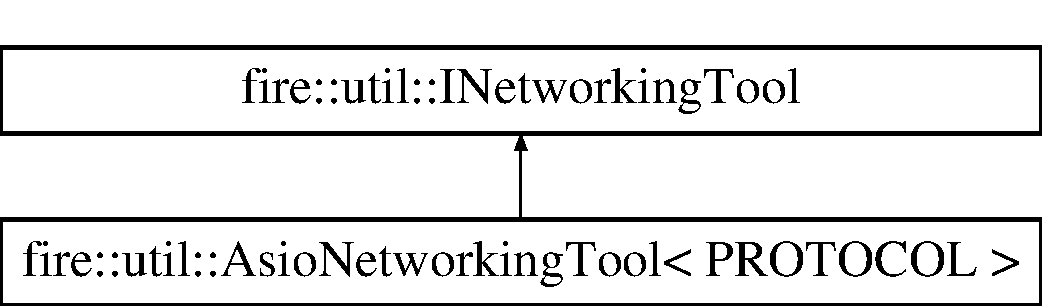
\includegraphics[height=2.000000cm]{a00994}
\end{center}
\end{figure}
\subsection*{Public Member Functions}
\begin{DoxyCompactItemize}
\item 
\hyperlink{a00994_a5edd72ce9937e052a82e7564500b3861}{Asio\+Networking\+Tool} (std\+::string host, int p)
\item 
\mbox{\Hypertarget{a00994_a5826de4a9e051ec854ad7be3a48ac86d}\label{a00994_a5826de4a9e051ec854ad7be3a48ac86d}} 
{\bfseries Asio\+Networking\+Tool} (std\+::string host\+\_\+and\+\_\+port, bool verify\+Cert=true, const std\+::string \&cert\+\_\+file=std\+::string(), const std\+::string \&private\+\_\+key\+\_\+file=std\+::string(), const std\+::string \&verify\+\_\+file=std\+::string())
\item 
virtual \hyperlink{a00994_afc51c728e1bd136b6729ac892df490ab}{$\sim$\+Asio\+Networking\+Tool} ()
\item 
virtual \hyperlink{a00998}{Http\+Response} \hyperlink{a00994_a42609f768f245acf0867889e920c5d49}{get} (const std\+::string \&relative\+Path, const std\+::map$<$ std\+::string, std\+::string $>$ \&header=std\+::map$<$ std\+::string, std\+::string $>$())
\item 
virtual \hyperlink{a00998}{Http\+Response} \hyperlink{a00994_a2ac524ceef89fceb928cf74420bf90a5}{post} (const std\+::string \&relative\+Path, const std\+::string \&message, const std\+::map$<$ std\+::string, std\+::string $>$ \&header=std\+::map$<$ std\+::string, std\+::string $>$())
\end{DoxyCompactItemize}
\subsection*{Protected Attributes}
\begin{DoxyCompactItemize}
\item 
std\+::shared\+\_\+ptr$<$ \hyperlink{a00934}{Web\+Client} $>$ \hyperlink{a00994_a57412dca950e86b857ee4795a9b6517e}{client}
\item 
\mbox{\Hypertarget{a00994_a613f571530390cf1d05538c658c13b9e}\label{a00994_a613f571530390cf1d05538c658c13b9e}} 
std\+::shared\+\_\+ptr$<$ Response\+Type $>$ {\bfseries response}
\end{DoxyCompactItemize}


\subsection{Detailed Description}
\subsubsection*{template$<$typename P\+R\+O\+T\+O\+C\+OL$>$\newline
class fire\+::util\+::\+Asio\+Networking\+Tool$<$ P\+R\+O\+T\+O\+C\+O\+L $>$}

The Asio\+Networkign\+Tool is a realization of the \hyperlink{a01002}{I\+Networking\+Tool} interface that uses the B\+O\+O\+ST Asio library to post/get http requests. 

\subsection{Constructor \& Destructor Documentation}
\mbox{\Hypertarget{a00994_a5edd72ce9937e052a82e7564500b3861}\label{a00994_a5edd72ce9937e052a82e7564500b3861}} 
\index{fire\+::util\+::\+Asio\+Networking\+Tool@{fire\+::util\+::\+Asio\+Networking\+Tool}!Asio\+Networking\+Tool@{Asio\+Networking\+Tool}}
\index{Asio\+Networking\+Tool@{Asio\+Networking\+Tool}!fire\+::util\+::\+Asio\+Networking\+Tool@{fire\+::util\+::\+Asio\+Networking\+Tool}}
\subsubsection{\texorpdfstring{Asio\+Networking\+Tool()}{AsioNetworkingTool()}}
{\footnotesize\ttfamily template$<$typename P\+R\+O\+T\+O\+C\+OL $>$ \\
\hyperlink{a00994}{fire\+::util\+::\+Asio\+Networking\+Tool}$<$ P\+R\+O\+T\+O\+C\+OL $>$\+::\hyperlink{a00994}{Asio\+Networking\+Tool} (\begin{DoxyParamCaption}\item[{std\+::string}]{host,  }\item[{int}]{p }\end{DoxyParamCaption})\hspace{0.3cm}{\ttfamily [inline]}}

The constructor \mbox{\Hypertarget{a00994_afc51c728e1bd136b6729ac892df490ab}\label{a00994_afc51c728e1bd136b6729ac892df490ab}} 
\index{fire\+::util\+::\+Asio\+Networking\+Tool@{fire\+::util\+::\+Asio\+Networking\+Tool}!````~Asio\+Networking\+Tool@{$\sim$\+Asio\+Networking\+Tool}}
\index{````~Asio\+Networking\+Tool@{$\sim$\+Asio\+Networking\+Tool}!fire\+::util\+::\+Asio\+Networking\+Tool@{fire\+::util\+::\+Asio\+Networking\+Tool}}
\subsubsection{\texorpdfstring{$\sim$\+Asio\+Networking\+Tool()}{~AsioNetworkingTool()}}
{\footnotesize\ttfamily template$<$typename P\+R\+O\+T\+O\+C\+OL $>$ \\
virtual \hyperlink{a00994}{fire\+::util\+::\+Asio\+Networking\+Tool}$<$ P\+R\+O\+T\+O\+C\+OL $>$\+::$\sim$\hyperlink{a00994}{Asio\+Networking\+Tool} (\begin{DoxyParamCaption}{ }\end{DoxyParamCaption})\hspace{0.3cm}{\ttfamily [inline]}, {\ttfamily [virtual]}}

The destructor 

\subsection{Member Function Documentation}
\mbox{\Hypertarget{a00994_a42609f768f245acf0867889e920c5d49}\label{a00994_a42609f768f245acf0867889e920c5d49}} 
\index{fire\+::util\+::\+Asio\+Networking\+Tool@{fire\+::util\+::\+Asio\+Networking\+Tool}!get@{get}}
\index{get@{get}!fire\+::util\+::\+Asio\+Networking\+Tool@{fire\+::util\+::\+Asio\+Networking\+Tool}}
\subsubsection{\texorpdfstring{get()}{get()}}
{\footnotesize\ttfamily template$<$typename P\+R\+O\+T\+O\+C\+OL $>$ \\
virtual \hyperlink{a00998}{Http\+Response} \hyperlink{a00994}{fire\+::util\+::\+Asio\+Networking\+Tool}$<$ P\+R\+O\+T\+O\+C\+OL $>$\+::get (\begin{DoxyParamCaption}\item[{const std\+::string \&}]{relative\+Path,  }\item[{const std\+::map$<$ std\+::string, std\+::string $>$ \&}]{header = {\ttfamily std\+:\+:map$<$~std\+:\+:string,~std\+:\+:string$>$()} }\end{DoxyParamCaption})\hspace{0.3cm}{\ttfamily [inline]}, {\ttfamily [virtual]}}

Return the last received status code.

\begin{DoxyReturn}{Returns}
code The status code as a string Issue an H\+T\+TP G\+ET Command at the given relative path. Clients can provide a map of header key values to modify the G\+ET request.
\end{DoxyReturn}

\begin{DoxyParams}{Parameters}
{\em relative\+Path} & The path relative to the hostname/port provided to this Networking\+Tool \\
\hline
\end{DoxyParams}
\begin{DoxyReturn}{Returns}
The contents at the U\+RL or an error message if one took place. 
\end{DoxyReturn}


Implements \hyperlink{a01002_a44b81ebf8421f0e32ed99b5e372ef007}{fire\+::util\+::\+I\+Networking\+Tool}.

\mbox{\Hypertarget{a00994_a2ac524ceef89fceb928cf74420bf90a5}\label{a00994_a2ac524ceef89fceb928cf74420bf90a5}} 
\index{fire\+::util\+::\+Asio\+Networking\+Tool@{fire\+::util\+::\+Asio\+Networking\+Tool}!post@{post}}
\index{post@{post}!fire\+::util\+::\+Asio\+Networking\+Tool@{fire\+::util\+::\+Asio\+Networking\+Tool}}
\subsubsection{\texorpdfstring{post()}{post()}}
{\footnotesize\ttfamily template$<$typename P\+R\+O\+T\+O\+C\+OL $>$ \\
virtual \hyperlink{a00998}{Http\+Response} \hyperlink{a00994}{fire\+::util\+::\+Asio\+Networking\+Tool}$<$ P\+R\+O\+T\+O\+C\+OL $>$\+::post (\begin{DoxyParamCaption}\item[{const std\+::string \&}]{relative\+Path,  }\item[{const std\+::string \&}]{message,  }\item[{const std\+::map$<$ std\+::string, std\+::string $>$ \&}]{header = {\ttfamily std\+:\+:map$<$~std\+:\+:string,~std\+:\+:string$>$()} }\end{DoxyParamCaption})\hspace{0.3cm}{\ttfamily [inline]}, {\ttfamily [virtual]}}

Issue an H\+T\+TP Post command at the given relative path with the provided message. Clients can provide a map of header key values to modify the P\+O\+ST request.


\begin{DoxyParams}{Parameters}
{\em relative\+Path} & The path relative to the hostname/port provided to this Networking\+Tool \\
\hline
{\em message} & The message to post \\
\hline
{\em header} & The map of additional H\+T\+TP P\+O\+ST header information \\
\hline
\end{DoxyParams}
\begin{DoxyReturn}{Returns}
success Boolean indicating if post was successful 
\end{DoxyReturn}


Implements \hyperlink{a01002_ad6ff0e352d78f17a6f6184d1b80e0c94}{fire\+::util\+::\+I\+Networking\+Tool}.



\subsection{Member Data Documentation}
\mbox{\Hypertarget{a00994_a57412dca950e86b857ee4795a9b6517e}\label{a00994_a57412dca950e86b857ee4795a9b6517e}} 
\index{fire\+::util\+::\+Asio\+Networking\+Tool@{fire\+::util\+::\+Asio\+Networking\+Tool}!client@{client}}
\index{client@{client}!fire\+::util\+::\+Asio\+Networking\+Tool@{fire\+::util\+::\+Asio\+Networking\+Tool}}
\subsubsection{\texorpdfstring{client}{client}}
{\footnotesize\ttfamily template$<$typename P\+R\+O\+T\+O\+C\+OL $>$ \\
std\+::shared\+\_\+ptr$<$\hyperlink{a00934}{Web\+Client}$>$ \hyperlink{a00994}{fire\+::util\+::\+Asio\+Networking\+Tool}$<$ P\+R\+O\+T\+O\+C\+OL $>$\+::client\hspace{0.3cm}{\ttfamily [protected]}}

Reference to the asio client we will use 

The documentation for this class was generated from the following file\+:\begin{DoxyCompactItemize}
\item 
Asio\+Networking\+Tool.\+hpp\end{DoxyCompactItemize}

\hypertarget{a00810}{}\section{Block\+Generator Struct Reference}
\label{a00810}\index{Block\+Generator@{Block\+Generator}}


The documentation for this struct was generated from the following file\+:\begin{DoxyCompactItemize}
\item 
I\+N\+I\+Property\+Parser\+Test.\+cpp\end{DoxyCompactItemize}

\hypertarget{a00926}{}\section{case\+\_\+insensitive\+\_\+equals Class Reference}
\label{a00926}\index{case\+\_\+insensitive\+\_\+equals@{case\+\_\+insensitive\+\_\+equals}}
\subsection*{Public Member Functions}
\begin{DoxyCompactItemize}
\item 
\mbox{\Hypertarget{a00926_a9d610611f775742c59898e6fa72c5808}\label{a00926_a9d610611f775742c59898e6fa72c5808}} 
bool {\bfseries operator()} (const std\+::string \&key1, const std\+::string \&key2) const
\item 
\mbox{\Hypertarget{a00926_a9d610611f775742c59898e6fa72c5808}\label{a00926_a9d610611f775742c59898e6fa72c5808}} 
bool {\bfseries operator()} (const std\+::string \&key1, const std\+::string \&key2) const
\end{DoxyCompactItemize}


The documentation for this class was generated from the following files\+:\begin{DoxyCompactItemize}
\item 
client\+\_\+http.\+hpp\item 
server\+\_\+http.\+hpp\end{DoxyCompactItemize}

\hypertarget{a00930}{}\section{case\+\_\+insensitive\+\_\+hash Class Reference}
\label{a00930}\index{case\+\_\+insensitive\+\_\+hash@{case\+\_\+insensitive\+\_\+hash}}
\subsection*{Public Member Functions}
\begin{DoxyCompactItemize}
\item 
\mbox{\Hypertarget{a00930_a4520cc9a7af6df84d9e81996d6473855}\label{a00930_a4520cc9a7af6df84d9e81996d6473855}} 
std\+::size\+\_\+t {\bfseries operator()} (const std\+::string \&key) const
\item 
\mbox{\Hypertarget{a00930_a67ee0c0a2bbecedb0d1aef29313de6a9}\label{a00930_a67ee0c0a2bbecedb0d1aef29313de6a9}} 
size\+\_\+t {\bfseries operator()} (const std\+::string \&key) const
\end{DoxyCompactItemize}


The documentation for this class was generated from the following files\+:\begin{DoxyCompactItemize}
\item 
client\+\_\+http.\+hpp\item 
server\+\_\+http.\+hpp\end{DoxyCompactItemize}

\hypertarget{a00934}{}\section{case\+\_\+insensitive\+\_\+equals Class Reference}
\label{a00934}\index{case\+\_\+insensitive\+\_\+equals@{case\+\_\+insensitive\+\_\+equals}}
\subsection*{Public Member Functions}
\begin{DoxyCompactItemize}
\item 
\mbox{\Hypertarget{a00934_a9d610611f775742c59898e6fa72c5808}\label{a00934_a9d610611f775742c59898e6fa72c5808}} 
bool {\bfseries operator()} (const std\+::string \&key1, const std\+::string \&key2) const
\item 
\mbox{\Hypertarget{a00934_a9d610611f775742c59898e6fa72c5808}\label{a00934_a9d610611f775742c59898e6fa72c5808}} 
bool {\bfseries operator()} (const std\+::string \&key1, const std\+::string \&key2) const
\end{DoxyCompactItemize}


The documentation for this class was generated from the following files\+:\begin{DoxyCompactItemize}
\item 
client\+\_\+http.\+hpp\item 
server\+\_\+http.\+hpp\end{DoxyCompactItemize}

\hypertarget{a00950}{}\section{Simple\+Web\+:\+:Client$<$ H\+T\+TP $>$ Class Template Reference}
\label{a00950}\index{Simple\+Web\+::\+Client$<$ H\+T\+T\+P $>$@{Simple\+Web\+::\+Client$<$ H\+T\+T\+P $>$}}
Inheritance diagram for Simple\+Web\+:\+:Client$<$ H\+T\+TP $>$\+:\begin{figure}[H]
\begin{center}
\leavevmode
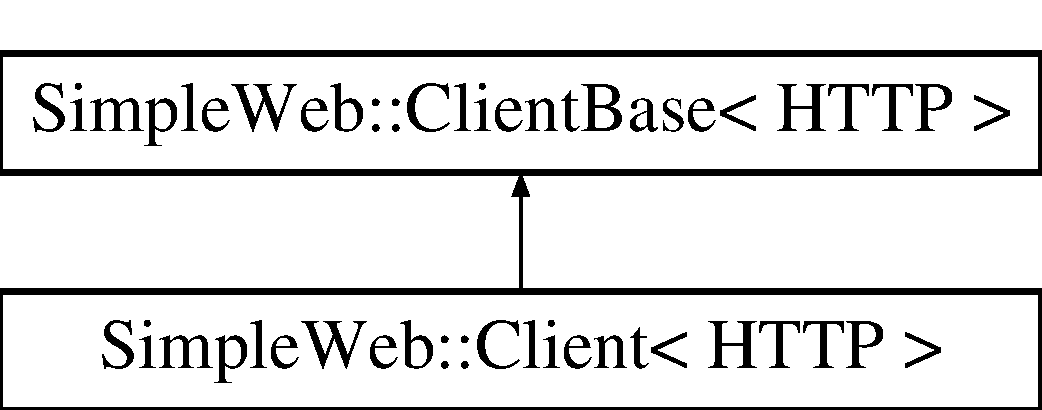
\includegraphics[height=2.000000cm]{a00950}
\end{center}
\end{figure}
\subsection*{Public Member Functions}
\begin{DoxyCompactItemize}
\item 
\mbox{\Hypertarget{a00950_a47655afc849e459096743876391dae17}\label{a00950_a47655afc849e459096743876391dae17}} 
{\bfseries Client} (const std\+::string \&server\+\_\+port\+\_\+path)
\end{DoxyCompactItemize}
\subsection*{Protected Member Functions}
\begin{DoxyCompactItemize}
\item 
\mbox{\Hypertarget{a00950_aebed110274c94b539e2d0a857c24991d}\label{a00950_aebed110274c94b539e2d0a857c24991d}} 
void {\bfseries connect} ()
\end{DoxyCompactItemize}
\subsection*{Additional Inherited Members}


The documentation for this class was generated from the following file\+:\begin{DoxyCompactItemize}
\item 
client\+\_\+http.\+hpp\end{DoxyCompactItemize}

\hypertarget{a00954}{}\section{Simple\+Web\+:\+:Client\+Base$<$ socket\+\_\+type $>$\+:\+:Config Class Reference}
\label{a00954}\index{Simple\+Web\+::\+Client\+Base$<$ socket\+\_\+type $>$\+::\+Config@{Simple\+Web\+::\+Client\+Base$<$ socket\+\_\+type $>$\+::\+Config}}
\subsection*{Public Attributes}
\begin{DoxyCompactItemize}
\item 
\mbox{\Hypertarget{a00954_ab0ec5665cc6666eb621e01e9403fdf28}\label{a00954_ab0ec5665cc6666eb621e01e9403fdf28}} 
std\+::size\+\_\+t \hyperlink{a00954_ab0ec5665cc6666eb621e01e9403fdf28}{timeout} = 0
\begin{DoxyCompactList}\small\item\em Set timeout on requests in seconds. Default value\+: 0 (no timeout). \end{DoxyCompactList}\item 
\mbox{\Hypertarget{a00954_ad810229c900c88c32ab42a8bfce2c4a1}\label{a00954_ad810229c900c88c32ab42a8bfce2c4a1}} 
std\+::size\+\_\+t \hyperlink{a00954_ad810229c900c88c32ab42a8bfce2c4a1}{timeout\+\_\+connect} = 0
\begin{DoxyCompactList}\small\item\em Set connect timeout in seconds. Default value\+: 0 (\hyperlink{a00954_ab0ec5665cc6666eb621e01e9403fdf28}{Config\+::timeout} is then used instead). \end{DoxyCompactList}\item 
\mbox{\Hypertarget{a00954_a6eb0382dccf50e9e8bdc541d3f06f9d5}\label{a00954_a6eb0382dccf50e9e8bdc541d3f06f9d5}} 
std\+::string \hyperlink{a00954_a6eb0382dccf50e9e8bdc541d3f06f9d5}{proxy\+\_\+server}
\begin{DoxyCompactList}\small\item\em Set proxy server (server\+:port) \end{DoxyCompactList}\end{DoxyCompactItemize}
\subsection*{Friends}
\begin{DoxyCompactItemize}
\item 
\mbox{\Hypertarget{a00954_aee5298660229dd276c7169cf7ef3d387}\label{a00954_aee5298660229dd276c7169cf7ef3d387}} 
class {\bfseries Client\+Base$<$ socket\+\_\+type $>$}
\end{DoxyCompactItemize}


The documentation for this class was generated from the following file\+:\begin{DoxyCompactItemize}
\item 
client\+\_\+http.\+hpp\end{DoxyCompactItemize}

\hypertarget{a00938}{}\section{case\+\_\+insensitive\+\_\+hash Class Reference}
\label{a00938}\index{case\+\_\+insensitive\+\_\+hash@{case\+\_\+insensitive\+\_\+hash}}
\subsection*{Public Member Functions}
\begin{DoxyCompactItemize}
\item 
\mbox{\Hypertarget{a00938_a4520cc9a7af6df84d9e81996d6473855}\label{a00938_a4520cc9a7af6df84d9e81996d6473855}} 
std\+::size\+\_\+t {\bfseries operator()} (const std\+::string \&key) const
\item 
\mbox{\Hypertarget{a00938_a67ee0c0a2bbecedb0d1aef29313de6a9}\label{a00938_a67ee0c0a2bbecedb0d1aef29313de6a9}} 
size\+\_\+t {\bfseries operator()} (const std\+::string \&key) const
\end{DoxyCompactItemize}


The documentation for this class was generated from the following files\+:\begin{DoxyCompactItemize}
\item 
client\+\_\+http.\+hpp\item 
server\+\_\+http.\+hpp\end{DoxyCompactItemize}

\hypertarget{a00946}{}\section{Simple\+Web\+:\+:Client\+Base$<$ socket\+\_\+type $>$ Class Template Reference}
\label{a00946}\index{Simple\+Web\+::\+Client\+Base$<$ socket\+\_\+type $>$@{Simple\+Web\+::\+Client\+Base$<$ socket\+\_\+type $>$}}
Inheritance diagram for Simple\+Web\+:\+:Client\+Base$<$ socket\+\_\+type $>$\+:\begin{figure}[H]
\begin{center}
\leavevmode
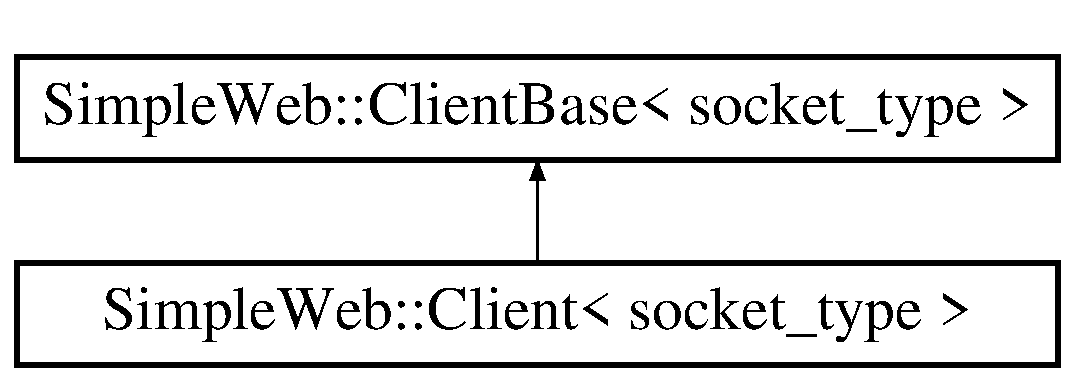
\includegraphics[height=2.000000cm]{a00946}
\end{center}
\end{figure}
\subsection*{Classes}
\begin{DoxyCompactItemize}
\item 
class \hyperlink{a00954}{Config}
\item 
class \hyperlink{a00950}{Response}
\end{DoxyCompactItemize}
\subsection*{Public Member Functions}
\begin{DoxyCompactItemize}
\item 
\mbox{\Hypertarget{a00946_ac8a838ace77f0a1a19b8cb03bdba7e74}\label{a00946_ac8a838ace77f0a1a19b8cb03bdba7e74}} 
std\+::shared\+\_\+ptr$<$ \hyperlink{a00950}{Response} $>$ {\bfseries request} (const std\+::string \&request\+\_\+type, const std\+::string \&path=\char`\"{}/\char`\"{}, boost\+::string\+\_\+ref content=\char`\"{}\char`\"{}, const std\+::map$<$ std\+::string, std\+::string $>$ \&header=std\+::map$<$ std\+::string, std\+::string $>$())
\item 
\mbox{\Hypertarget{a00946_aca6cb17dbea9adf0cf1daf9d1ea70f76}\label{a00946_aca6cb17dbea9adf0cf1daf9d1ea70f76}} 
std\+::shared\+\_\+ptr$<$ \hyperlink{a00950}{Response} $>$ {\bfseries request} (const std\+::string \&request\+\_\+type, const std\+::string \&path, std\+::iostream \&content, const std\+::map$<$ std\+::string, std\+::string $>$ \&header=std\+::map$<$ std\+::string, std\+::string $>$())
\item 
\mbox{\Hypertarget{a00946_ad21735a9bda2fae6aedd811efae981e1}\label{a00946_ad21735a9bda2fae6aedd811efae981e1}} 
void {\bfseries close} ()
\end{DoxyCompactItemize}
\subsection*{Public Attributes}
\begin{DoxyCompactItemize}
\item 
\mbox{\Hypertarget{a00946_af17ddd25319c4f9029969441dfd54eff}\label{a00946_af17ddd25319c4f9029969441dfd54eff}} 
\hyperlink{a00954}{Config} \hyperlink{a00946_af17ddd25319c4f9029969441dfd54eff}{config}
\begin{DoxyCompactList}\small\item\em Set before calling request. \end{DoxyCompactList}\end{DoxyCompactItemize}
\subsection*{Protected Member Functions}
\begin{DoxyCompactItemize}
\item 
\mbox{\Hypertarget{a00946_a4a74d44c9df44d0d469ad453bdac43bf}\label{a00946_a4a74d44c9df44d0d469ad453bdac43bf}} 
{\bfseries Client\+Base} (const std\+::string \&host\+\_\+port, unsigned short default\+\_\+port)
\item 
\mbox{\Hypertarget{a00946_ac511a8e5de870f533f8c28270c82dbfa}\label{a00946_ac511a8e5de870f533f8c28270c82dbfa}} 
std\+::pair$<$ std\+::string, unsigned short $>$ {\bfseries parse\+\_\+host\+\_\+port} (const std\+::string \&host\+\_\+port, unsigned short default\+\_\+port)
\item 
\mbox{\Hypertarget{a00946_a4c1f364a57eaef8fd10c29a82e475010}\label{a00946_a4c1f364a57eaef8fd10c29a82e475010}} 
virtual void {\bfseries connect} ()=0
\item 
\mbox{\Hypertarget{a00946_ab76f469e8f909bf046a80d5afad70469}\label{a00946_ab76f469e8f909bf046a80d5afad70469}} 
std\+::shared\+\_\+ptr$<$ boost\+::asio\+::deadline\+\_\+timer $>$ {\bfseries get\+\_\+timeout\+\_\+timer} (std\+::size\+\_\+t timeout=0)
\item 
\mbox{\Hypertarget{a00946_af11668a7cbf1a4e51f694c853cb70afe}\label{a00946_af11668a7cbf1a4e51f694c853cb70afe}} 
void {\bfseries parse\+\_\+response\+\_\+header} (const std\+::shared\+\_\+ptr$<$ \hyperlink{a00950}{Response} $>$ \&response) const
\item 
\mbox{\Hypertarget{a00946_afa5ddce26ed4c7570a764e2ff003fa25}\label{a00946_afa5ddce26ed4c7570a764e2ff003fa25}} 
std\+::shared\+\_\+ptr$<$ \hyperlink{a00950}{Response} $>$ {\bfseries request\+\_\+read} ()
\item 
\mbox{\Hypertarget{a00946_ae7fa171a9555114e702cafb3f85bc7d5}\label{a00946_ae7fa171a9555114e702cafb3f85bc7d5}} 
void {\bfseries request\+\_\+read\+\_\+chunked} (const std\+::shared\+\_\+ptr$<$ \hyperlink{a00950}{Response} $>$ \&response, boost\+::asio\+::streambuf \&streambuf)
\end{DoxyCompactItemize}
\subsection*{Protected Attributes}
\begin{DoxyCompactItemize}
\item 
\mbox{\Hypertarget{a00946_abe07c05fed46efc9e6aa76736961ae20}\label{a00946_abe07c05fed46efc9e6aa76736961ae20}} 
boost\+::asio\+::io\+\_\+service {\bfseries io\+\_\+service}
\item 
\mbox{\Hypertarget{a00946_a2001dc43f4c3ef1f07a86eea8fbf8082}\label{a00946_a2001dc43f4c3ef1f07a86eea8fbf8082}} 
boost\+::asio\+::ip\+::tcp\+::resolver {\bfseries resolver}
\item 
\mbox{\Hypertarget{a00946_a48b0e61c61cfc3d5307a0101cc30a28e}\label{a00946_a48b0e61c61cfc3d5307a0101cc30a28e}} 
std\+::unique\+\_\+ptr$<$ socket\+\_\+type $>$ {\bfseries socket}
\item 
\mbox{\Hypertarget{a00946_a2c0d5c3d38f4a6a21b67918199b498da}\label{a00946_a2c0d5c3d38f4a6a21b67918199b498da}} 
std\+::mutex {\bfseries socket\+\_\+mutex}
\item 
\mbox{\Hypertarget{a00946_a4436f29ffdce0b29b210cbecd972ffef}\label{a00946_a4436f29ffdce0b29b210cbecd972ffef}} 
std\+::string {\bfseries host}
\item 
\mbox{\Hypertarget{a00946_aadd3336b64a1f8d559af656554ddd0e9}\label{a00946_aadd3336b64a1f8d559af656554ddd0e9}} 
unsigned short {\bfseries port}
\end{DoxyCompactItemize}


The documentation for this class was generated from the following file\+:\begin{DoxyCompactItemize}
\item 
client\+\_\+http.\+hpp\end{DoxyCompactItemize}

\hypertarget{a00978}{}\section{Simple\+Web\+:\+:Server\+Base$<$ socket\+\_\+type $>$\+:\+:Config Class Reference}
\label{a00978}\index{Simple\+Web\+::\+Server\+Base$<$ socket\+\_\+type $>$\+::\+Config@{Simple\+Web\+::\+Server\+Base$<$ socket\+\_\+type $>$\+::\+Config}}
\subsection*{Public Attributes}
\begin{DoxyCompactItemize}
\item 
\mbox{\Hypertarget{a00978_aa80030952ff056db08f736d5537bd2c9}\label{a00978_aa80030952ff056db08f736d5537bd2c9}} 
unsigned short \hyperlink{a00978_aa80030952ff056db08f736d5537bd2c9}{port}
\begin{DoxyCompactList}\small\item\em Port number to use. Defaults to 80 for H\+T\+TP and 443 for H\+T\+T\+PS. \end{DoxyCompactList}\item 
\mbox{\Hypertarget{a00978_abfbbfc38bfd2887739676424509dbb45}\label{a00978_abfbbfc38bfd2887739676424509dbb45}} 
size\+\_\+t \hyperlink{a00978_abfbbfc38bfd2887739676424509dbb45}{thread\+\_\+pool\+\_\+size} =1
\begin{DoxyCompactList}\small\item\em Number of threads that the server will use when start() is called. Defaults to 1 thread. \end{DoxyCompactList}\item 
\mbox{\Hypertarget{a00978_aa27e09c83d7e26dff6e72e8d1084d5a0}\label{a00978_aa27e09c83d7e26dff6e72e8d1084d5a0}} 
size\+\_\+t \hyperlink{a00978_aa27e09c83d7e26dff6e72e8d1084d5a0}{timeout\+\_\+request} =5
\begin{DoxyCompactList}\small\item\em Timeout on request handling. Defaults to 5 seconds. \end{DoxyCompactList}\item 
\mbox{\Hypertarget{a00978_ac1f74ff91196c3a72446786b54a77b58}\label{a00978_ac1f74ff91196c3a72446786b54a77b58}} 
size\+\_\+t \hyperlink{a00978_ac1f74ff91196c3a72446786b54a77b58}{timeout\+\_\+content} =300
\begin{DoxyCompactList}\small\item\em Timeout on content handling. Defaults to 300 seconds. \end{DoxyCompactList}\item 
std\+::string \hyperlink{a00978_add7a705aca3533bf0371708b19bb691c}{address}
\item 
\mbox{\Hypertarget{a00978_aab9c347da5390b176d37dac2dfbd9fae}\label{a00978_aab9c347da5390b176d37dac2dfbd9fae}} 
bool \hyperlink{a00978_aab9c347da5390b176d37dac2dfbd9fae}{reuse\+\_\+address} =true
\begin{DoxyCompactList}\small\item\em Set to false to avoid binding the socket to an address that is already in use. Defaults to true. \end{DoxyCompactList}\end{DoxyCompactItemize}
\subsection*{Friends}
\begin{DoxyCompactItemize}
\item 
\mbox{\Hypertarget{a00978_a01d54a7e16ca437c98ec571deca98dfc}\label{a00978_a01d54a7e16ca437c98ec571deca98dfc}} 
class {\bfseries Server\+Base$<$ socket\+\_\+type $>$}
\end{DoxyCompactItemize}


\subsection{Member Data Documentation}
\mbox{\Hypertarget{a00978_add7a705aca3533bf0371708b19bb691c}\label{a00978_add7a705aca3533bf0371708b19bb691c}} 
\index{Simple\+Web\+::\+Server\+Base\+::\+Config@{Simple\+Web\+::\+Server\+Base\+::\+Config}!address@{address}}
\index{address@{address}!Simple\+Web\+::\+Server\+Base\+::\+Config@{Simple\+Web\+::\+Server\+Base\+::\+Config}}
\subsubsection{\texorpdfstring{address}{address}}
{\footnotesize\ttfamily template$<$class socket\+\_\+type$>$ \\
std\+::string \hyperlink{a00962}{Simple\+Web\+::\+Server\+Base}$<$ socket\+\_\+type $>$\+::Config\+::address}

I\+Pv4 address in dotted decimal form or I\+Pv6 address in hexadecimal notation. If empty, the address will be any address. 

The documentation for this class was generated from the following file\+:\begin{DoxyCompactItemize}
\item 
server\+\_\+http.\+hpp\end{DoxyCompactItemize}

\hypertarget{a00970}{}\section{Simple\+Web\+:\+:Server\+Base$<$ socket\+\_\+type $>$\+:\+:Content Class Reference}
\label{a00970}\index{Simple\+Web\+::\+Server\+Base$<$ socket\+\_\+type $>$\+::\+Content@{Simple\+Web\+::\+Server\+Base$<$ socket\+\_\+type $>$\+::\+Content}}
Inheritance diagram for Simple\+Web\+:\+:Server\+Base$<$ socket\+\_\+type $>$\+:\+:Content\+:\begin{figure}[H]
\begin{center}
\leavevmode
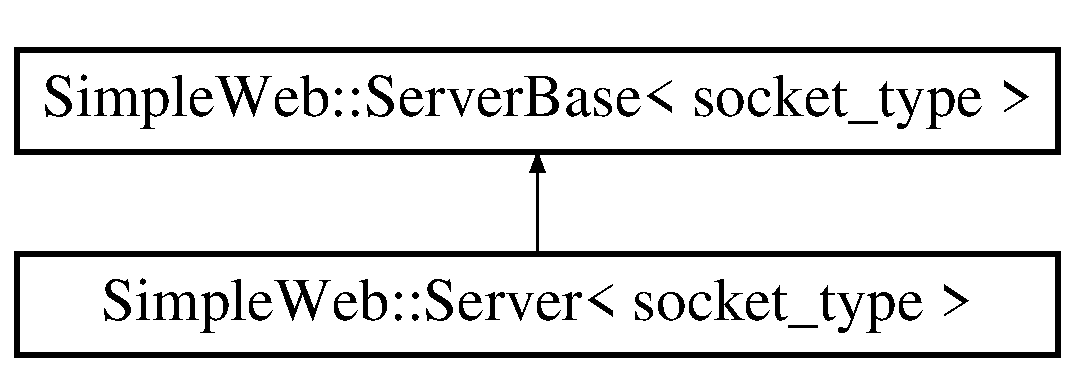
\includegraphics[height=5.000000cm]{a00970}
\end{center}
\end{figure}
\subsection*{Public Member Functions}
\begin{DoxyCompactItemize}
\item 
\mbox{\Hypertarget{a00970_adf8b2386c8ab32277341c6ae07cd4670}\label{a00970_adf8b2386c8ab32277341c6ae07cd4670}} 
size\+\_\+t {\bfseries size} ()
\item 
\mbox{\Hypertarget{a00970_a6b4a72b0631c88ef576db28f54a768cb}\label{a00970_a6b4a72b0631c88ef576db28f54a768cb}} 
std\+::string {\bfseries string} ()
\end{DoxyCompactItemize}
\subsection*{Friends}
\begin{DoxyCompactItemize}
\item 
\mbox{\Hypertarget{a00970_a01d54a7e16ca437c98ec571deca98dfc}\label{a00970_a01d54a7e16ca437c98ec571deca98dfc}} 
class {\bfseries Server\+Base$<$ socket\+\_\+type $>$}
\end{DoxyCompactItemize}


The documentation for this class was generated from the following file\+:\begin{DoxyCompactItemize}
\item 
server\+\_\+http.\+hpp\end{DoxyCompactItemize}

\hypertarget{a00902}{}\section{C\+Simple\+Ini\+Templ$<$ S\+I\+\_\+\+C\+H\+AR, S\+I\+\_\+\+S\+T\+R\+L\+E\+SS, S\+I\+\_\+\+C\+O\+N\+V\+E\+R\+T\+ER $>$\+:\+:Converter Class Reference}
\label{a00902}\index{C\+Simple\+Ini\+Templ$<$ S\+I\+\_\+\+C\+H\+A\+R, S\+I\+\_\+\+S\+T\+R\+L\+E\+S\+S, S\+I\+\_\+\+C\+O\+N\+V\+E\+R\+T\+E\+R $>$\+::\+Converter@{C\+Simple\+Ini\+Templ$<$ S\+I\+\_\+\+C\+H\+A\+R, S\+I\+\_\+\+S\+T\+R\+L\+E\+S\+S, S\+I\+\_\+\+C\+O\+N\+V\+E\+R\+T\+E\+R $>$\+::\+Converter}}


{\ttfamily \#include $<$Simple\+Ini.\+h$>$}

Inheritance diagram for C\+Simple\+Ini\+Templ$<$ S\+I\+\_\+\+C\+H\+AR, S\+I\+\_\+\+S\+T\+R\+L\+E\+SS, S\+I\+\_\+\+C\+O\+N\+V\+E\+R\+T\+ER $>$\+:\+:Converter\+:\begin{figure}[H]
\begin{center}
\leavevmode
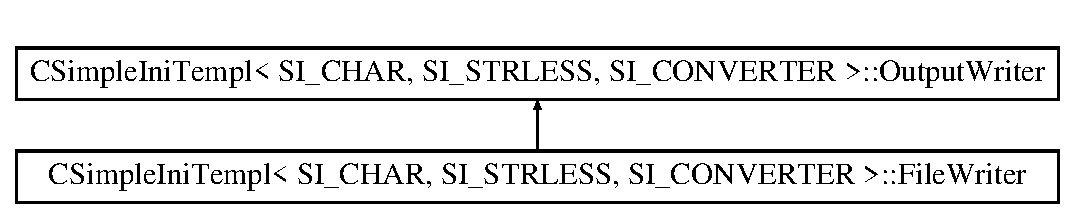
\includegraphics[height=2.000000cm]{a00902}
\end{center}
\end{figure}
\subsection*{Public Member Functions}
\begin{DoxyCompactItemize}
\item 
\mbox{\Hypertarget{a00902_ab8e740b211e4ece127d4d25773ba7e42}\label{a00902_ab8e740b211e4ece127d4d25773ba7e42}} 
{\bfseries Converter} (bool a\+\_\+b\+Store\+Is\+Utf8)
\item 
\mbox{\Hypertarget{a00902_a2f6e993014ed5d60c6e890e55beb0805}\label{a00902_a2f6e993014ed5d60c6e890e55beb0805}} 
{\bfseries Converter} (const \hyperlink{a00902}{Converter} \&rhs)
\item 
\mbox{\Hypertarget{a00902_af858c01c6a7e4ce9fafd18abc9e0ac1b}\label{a00902_af858c01c6a7e4ce9fafd18abc9e0ac1b}} 
\hyperlink{a00902}{Converter} \& {\bfseries operator=} (const \hyperlink{a00902}{Converter} \&rhs)
\item 
\mbox{\Hypertarget{a00902_a4e4186867214b54326cf622e323c9f2f}\label{a00902_a4e4186867214b54326cf622e323c9f2f}} 
bool {\bfseries Convert\+To\+Store} (const S\+I\+\_\+\+C\+H\+AR $\ast$a\+\_\+psz\+String)
\item 
\mbox{\Hypertarget{a00902_a918bbd4f861a2872e148bc9481ac80bb}\label{a00902_a918bbd4f861a2872e148bc9481ac80bb}} 
const char $\ast$ {\bfseries Data} ()
\end{DoxyCompactItemize}


\subsection{Detailed Description}
\subsubsection*{template$<$class S\+I\+\_\+\+C\+H\+AR, class S\+I\+\_\+\+S\+T\+R\+L\+E\+SS, class S\+I\+\_\+\+C\+O\+N\+V\+E\+R\+T\+ER$>$\newline
class C\+Simple\+Ini\+Templ$<$ S\+I\+\_\+\+C\+H\+A\+R, S\+I\+\_\+\+S\+T\+R\+L\+E\+S\+S, S\+I\+\_\+\+C\+O\+N\+V\+E\+R\+T\+E\+R $>$\+::\+Converter}

Characterset conversion utility class to convert strings to the same format as is used for the storage. 

The documentation for this class was generated from the following file\+:\begin{DoxyCompactItemize}
\item 
Simple\+Ini.\+h\end{DoxyCompactItemize}

\hypertarget{a00874}{}\section{fire\+:\+:State$<$ T $>$ Class Template Reference}
\label{a00874}\index{fire\+::\+State$<$ T $>$@{fire\+::\+State$<$ T $>$}}


{\ttfamily \#include $<$State.\+h$>$}

\subsection*{Public Member Functions}
\begin{DoxyCompactItemize}
\item 
\hyperlink{a00874_a697d926ef53bfa150fdabb31db269c21}{State} ()
\item 
\hyperlink{a00874_a40fd4082cd305e2054208a0b9aaa6ad4}{State} (const long \&num\+Elements)
\item 
\hyperlink{a00874_a7ca4384c9350a172f8e99cd60ae3e8f8}{State} (T domain\+State)
\item 
\hyperlink{a00874_a4d31866ba56d0017805f2065eb3302a3}{State} (T domain\+State, const long \&num\+Elements)
\item 
void \hyperlink{a00874_adfb16dbbaab3549c09da734605f815a3}{add\+Monitor} (std\+::function$<$ void(\hyperlink{a00874}{State}$<$ T $>$ \&)$>$ monitor)
\item 
T \& \hyperlink{a00874_a79792c7af9513986cb97627054c26edf}{get} ()
\item 
void \hyperlink{a00874_a5d8acc4d5bdd8942de10d34c55680349}{t} (double t)
\item 
const double \& \hyperlink{a00874_a425a0236c4edc506b30196d352118104}{t} () const
\item 
double $\ast$ \hyperlink{a00874_a3b811d98a73f53fd9b3901a10ec793da}{u} ()
\item 
void \hyperlink{a00874_a1b6b91c51fe4d53f268a33c77fecff11}{u} (double $\ast$data)
\item 
double $\ast$ \hyperlink{a00874_a8512e68bd6c39042eeede06dc58d390d}{dudt} (const double \&\hyperlink{a00874_a5d8acc4d5bdd8942de10d34c55680349}{t})
\item 
void \hyperlink{a00874_a22b2d9e2feb153c819e90a4ac7ee8d72}{size} (const long \&num\+Elements)
\item 
int \hyperlink{a00874_a19f1d7b5ce637db79b96f29bd146842a}{size} () const
\item 
{\footnotesize template$<$$>$ }\\double $\ast$ \hyperlink{a00874_abfc1fcd953b86552fb9e2b6c15baef6d}{u} ()
\item 
\mbox{\Hypertarget{a00874_a2a3ffc947a9658d7e7173591460d9424}\label{a00874_a2a3ffc947a9658d7e7173591460d9424}} 
{\footnotesize template$<$$>$ }\\void {\bfseries u} (double $\ast$u\+Data)
\item 
\mbox{\Hypertarget{a00874_aaaf6b9e3906f1c61bcfbd3df518352f8}\label{a00874_aaaf6b9e3906f1c61bcfbd3df518352f8}} 
{\footnotesize template$<$$>$ }\\double $\ast$ {\bfseries dudt} (const double \&\hyperlink{a00874_a5d8acc4d5bdd8942de10d34c55680349}{t})
\item 
\mbox{\Hypertarget{a00874_a075464a65d420579b91253e4eee1c238}\label{a00874_a075464a65d420579b91253e4eee1c238}} 
{\footnotesize template$<$$>$ }\\double $\ast$ {\bfseries u} ()
\item 
\mbox{\Hypertarget{a00874_a70019e1e9e42f93a40b99c79e1e0df8d}\label{a00874_a70019e1e9e42f93a40b99c79e1e0df8d}} 
{\footnotesize template$<$$>$ }\\double $\ast$ {\bfseries dudt} (const double \&\hyperlink{a00874_a5d8acc4d5bdd8942de10d34c55680349}{t})
\item 
\mbox{\Hypertarget{a00874_a075464a65d420579b91253e4eee1c238}\label{a00874_a075464a65d420579b91253e4eee1c238}} 
{\footnotesize template$<$$>$ }\\double $\ast$ {\bfseries u} ()
\item 
\mbox{\Hypertarget{a00874_a70019e1e9e42f93a40b99c79e1e0df8d}\label{a00874_a70019e1e9e42f93a40b99c79e1e0df8d}} 
{\footnotesize template$<$$>$ }\\double $\ast$ {\bfseries dudt} (const double \&\hyperlink{a00874_a5d8acc4d5bdd8942de10d34c55680349}{t})
\end{DoxyCompactItemize}
\subsection*{Protected Member Functions}
\begin{DoxyCompactItemize}
\item 
void \hyperlink{a00874_ad271749a2a4f73c11e82ae28141d3b65}{notify\+Monitors} ()
\end{DoxyCompactItemize}
\subsection*{Protected Attributes}
\begin{DoxyCompactItemize}
\item 
T \hyperlink{a00874_ac0008054a4c1e589bcbf17b9057daa41}{state}
\item 
double \hyperlink{a00874_a4985617940993cea772a7fc977c87237}{t\+Val}
\item 
long \hyperlink{a00874_a08f8f4ea745ae855ef730896efabf1ae}{system\+Size}
\item 
std\+::unique\+\_\+ptr$<$ double $>$ \hyperlink{a00874_aae89d6e350df763d503d7da862f1f30a}{u\+Arr}
\item 
std\+::unique\+\_\+ptr$<$ double $>$ \hyperlink{a00874_a9954ba8c1a12555ca1bf67b6a2bf2b3b}{dudt\+Arr}
\item 
std\+::vector$<$ std\+::function$<$ void(\hyperlink{a00874}{State}$<$ T $>$ \&)$>$ $>$ \hyperlink{a00874_ae1571b0a1c82060e525ce6ce2119ae5e}{monitors}
\end{DoxyCompactItemize}


\subsection{Detailed Description}
\subsubsection*{template$<$typename T$>$\newline
class fire\+::\+State$<$ T $>$}

This is a container class for user-\/provided data structures that can be passed to solvers. It is designed such that container operations are handled by default by the template and clients override the \hyperlink{a00874_a3b811d98a73f53fd9b3901a10ec793da}{u()} and \hyperlink{a00874_a8512e68bd6c39042eeede06dc58d390d}{dudt()} operations to tailor the behavior for the templated type.

Instances should be constructed using the \hyperlink{a00195_abca66b4f2a1543308b663714bd8b4855}{build$<$$>$()} templates as follows\+: 
\begin{DoxyCode}
State<T> myState = build<T>(); \textcolor{comment}{// If T() takes no arguments}
State<T> myState2 = build<T,int>(); \textcolor{comment}{// If T takes one argument}
State<T> myState3 = build<T,int, const double &>(); \textcolor{comment}{// If T takes 2 args}
\textcolor{comment}{//...etc.}
\end{DoxyCode}


The variable t, when discussed below, is meant to represent a free parameter on which u and du depend. It commonly represents time, but might might also represent some other parameter. It is not explicitly called \char`\"{}time\char`\"{} to keep the interface clean of any concepts that might limit the scope of the class to only data that is used in time integrations, when in fact it can be used in the solution of any initial value problem.

The layout of the state is, in effect, a matrix with size n\+\_\+e $\ast$ n\+\_\+t, where n\+\_\+e is the number of unique elements (or unknowns) considered in the system and n\+\_\+t is the number of values of t at which those values are considered. Thus, in the case where a problem has six unknowns (n\+\_\+e = 6) and fifty time steps (t = time and n\+\_\+t = 50), the state class could represent a 6 x 50 matrix with a total of 300 elements. Note that whether or not \char`\"{}the matrix\char`\"{} is stored in column or row major format is not important.

This class is designed to be greedy and narcissistic. In lieu of allowing users to create and store their own instances of T, it creates (add()) those instances and forces users to interact with references retrieved using the getters. Being so greedy makes it possible for this class to efficiently manage memory with lower implementation overhead and no need to rely on clients to correctly initialize data. The original design of this class called for extensive use of smart pointers (using std\+::share), but there are few computational advantages -\/ if any -\/ compared to simple references. This is because simple references do not incur atomic increment and decrement costs when crossing function boundaries, but smart pointers do. In the author\textquotesingle{}s personal experience, the cost of working with smart pointers can be as much as a factor of two in tight loops with function boundaries. References are, by comparison, free in tight loops. Alternatively, passing a reference to the smart pointer is also free, but it is hardly necessary to share a smart pointer at all if the client does not need to participate in the memory lifecycle of the class, and indeed the practice is not recommended (c.\+f. -\/ Sutter\textquotesingle{}s 2014 talk) at all in that case.

Three operations are provided for working with \char`\"{}fundamental state
vectors\char`\"{} as arrays of doubles, but casual users are warned that these operations are for those implementing fast solvers based on this class and, in general, casual users should stick to add() and \hyperlink{a00874_a79792c7af9513986cb97627054c26edf}{get()}.

\hyperlink{a00874}{State} objects can be monitored by registering a functor with the \hyperlink{a00874_adfb16dbbaab3549c09da734605f815a3}{add\+Monitor()} operation. The simplest example is to use a Lambda as follows\+: 
\begin{DoxyCode}
   \textcolor{comment}{// Register an observer to write a message when the state changes.}
state.add([](State<ReactionNetwork> & state) \{
   std::cout << \textcolor{stringliteral}{"Lambda Test "} << state.t() << std::endl;
   \textcolor{keywordflow}{return};
\});
\end{DoxyCode}
 Monitors are only called when \hyperlink{a00874_a1b6b91c51fe4d53f268a33c77fecff11}{u(double $\ast$)} is called. Classes that create explicit specializations of that function should call \hyperlink{a00874_ad271749a2a4f73c11e82ae28141d3b65}{notify\+Monitors()}, a protected notification function, to notify the monitors if they require that functionality. Simply calling the \hyperlink{a00874_ad271749a2a4f73c11e82ae28141d3b65}{notify\+Monitors()} function immediately before return is sufficient.

This class does not yet consider thread safety issues when calling the monitors or updating the state, so be warned.

Common Errors\+: Declaring T instead of T\& -\/ The C++ compiler will not throw an error in the following scenario and will create a copy instead\+: 
\begin{DoxyCode}
T myT1 = state.get(); \textcolor{comment}{// WRONG - Creates a copy of the state!}
T & myT2 = state.get(); \textcolor{comment}{// Correct - Uses the state by reference.}
\textcolor{keyword}{auto} myT3 = state.get(); \textcolor{comment}{// WRONG - Same as the first case.}
\textcolor{keyword}{auto} & myT4 = state.get(); \textcolor{comment}{// Correct - Same as the second case.}
\end{DoxyCode}


Road Map\+:
\begin{DoxyItemize}
\item Right now the auxilliary storage buffers u\+Arr and udt\+Arr are always allocated. It should be possible to enable or disable this.
\item Should this be thread safe?
\item Would be interesting to name monitors. 
\end{DoxyItemize}

\subsection{Constructor \& Destructor Documentation}
\mbox{\Hypertarget{a00874_a697d926ef53bfa150fdabb31db269c21}\label{a00874_a697d926ef53bfa150fdabb31db269c21}} 
\index{fire\+::\+State@{fire\+::\+State}!State@{State}}
\index{State@{State}!fire\+::\+State@{fire\+::\+State}}
\subsubsection{\texorpdfstring{State()}{State()}\hspace{0.1cm}{\footnotesize\ttfamily [1/4]}}
{\footnotesize\ttfamily template$<$typename T$>$ \\
\hyperlink{a00874}{fire\+::\+State}$<$ T $>$\+::\hyperlink{a00874}{State} (\begin{DoxyParamCaption}{ }\end{DoxyParamCaption})\hspace{0.3cm}{\ttfamily [inline]}}

Constructor \mbox{\Hypertarget{a00874_a40fd4082cd305e2054208a0b9aaa6ad4}\label{a00874_a40fd4082cd305e2054208a0b9aaa6ad4}} 
\index{fire\+::\+State@{fire\+::\+State}!State@{State}}
\index{State@{State}!fire\+::\+State@{fire\+::\+State}}
\subsubsection{\texorpdfstring{State()}{State()}\hspace{0.1cm}{\footnotesize\ttfamily [2/4]}}
{\footnotesize\ttfamily template$<$typename T$>$ \\
\hyperlink{a00874}{fire\+::\+State}$<$ T $>$\+::\hyperlink{a00874}{State} (\begin{DoxyParamCaption}\item[{const long \&}]{num\+Elements }\end{DoxyParamCaption})\hspace{0.3cm}{\ttfamily [inline]}}

Alternative constructor that also sets the system size. 
\begin{DoxyParams}{Parameters}
{\em the} & number of unique data elements in the state \\
\hline
\end{DoxyParams}
\mbox{\Hypertarget{a00874_a7ca4384c9350a172f8e99cd60ae3e8f8}\label{a00874_a7ca4384c9350a172f8e99cd60ae3e8f8}} 
\index{fire\+::\+State@{fire\+::\+State}!State@{State}}
\index{State@{State}!fire\+::\+State@{fire\+::\+State}}
\subsubsection{\texorpdfstring{State()}{State()}\hspace{0.1cm}{\footnotesize\ttfamily [3/4]}}
{\footnotesize\ttfamily template$<$typename T$>$ \\
\hyperlink{a00874}{fire\+::\+State}$<$ T $>$\+::\hyperlink{a00874}{State} (\begin{DoxyParamCaption}\item[{T}]{domain\+State }\end{DoxyParamCaption})\hspace{0.3cm}{\ttfamily [inline]}}

An alternative default constructor that will accept a pre-\/configured unique\+\_\+ptr$<$\+T$>$. In general this constructor should not be called directly by clients. It is used by the \hyperlink{a00195_abca66b4f2a1543308b663714bd8b4855}{build$<$$>$()} builder for State$<$\+T$>$ to safely and easily enable two-\/phase construction where the arguments can be passed to T\textquotesingle{}s constructor without requiring State$<$\+T$>$ to know about those arguments.

This is important because requiring State$<$\+T$>$ to know about the arguments of T\textquotesingle{}s constructor would require declaring those arguments in all client classes of State$<$\+T$>$ that used that version of T, which is an undue burden on the user compared to safely enabling two-\/phase construction. \mbox{\Hypertarget{a00874_a4d31866ba56d0017805f2065eb3302a3}\label{a00874_a4d31866ba56d0017805f2065eb3302a3}} 
\index{fire\+::\+State@{fire\+::\+State}!State@{State}}
\index{State@{State}!fire\+::\+State@{fire\+::\+State}}
\subsubsection{\texorpdfstring{State()}{State()}\hspace{0.1cm}{\footnotesize\ttfamily [4/4]}}
{\footnotesize\ttfamily template$<$typename T$>$ \\
\hyperlink{a00874}{fire\+::\+State}$<$ T $>$\+::\hyperlink{a00874}{State} (\begin{DoxyParamCaption}\item[{T}]{domain\+State,  }\item[{const long \&}]{num\+Elements }\end{DoxyParamCaption})\hspace{0.3cm}{\ttfamily [inline]}}

An alternative constructor that also sets the system size. Analog of \hyperlink{a00874_a40fd4082cd305e2054208a0b9aaa6ad4}{State(const long \&)}. 

\subsection{Member Function Documentation}
\mbox{\Hypertarget{a00874_adfb16dbbaab3549c09da734605f815a3}\label{a00874_adfb16dbbaab3549c09da734605f815a3}} 
\index{fire\+::\+State@{fire\+::\+State}!add\+Monitor@{add\+Monitor}}
\index{add\+Monitor@{add\+Monitor}!fire\+::\+State@{fire\+::\+State}}
\subsubsection{\texorpdfstring{add\+Monitor()}{addMonitor()}}
{\footnotesize\ttfamily template$<$typename T$>$ \\
void \hyperlink{a00874}{fire\+::\+State}$<$ T $>$\+::add\+Monitor (\begin{DoxyParamCaption}\item[{std\+::function$<$ void(\hyperlink{a00874}{State}$<$ T $>$ \&)$>$}]{monitor }\end{DoxyParamCaption})\hspace{0.3cm}{\ttfamily [inline]}}

This operation registers a function with the state that will be called when the state changes. Multiple functions may be registered with the \hyperlink{a00874}{State} and each will be notified when the state is modified. The monitor may be implemented in many ways, but should only take a single State$<$\+T$>$\& as an input an return void.

When the monitoring function is called, it will be passed a reference to the instance of the \hyperlink{a00874}{State} class that changed, not merely to the maintained type. 
\begin{DoxyParams}{Parameters}
{\em monitor} & the functor that should be notified when the state changes. \\
\hline
\end{DoxyParams}
\mbox{\Hypertarget{a00874_a8512e68bd6c39042eeede06dc58d390d}\label{a00874_a8512e68bd6c39042eeede06dc58d390d}} 
\index{fire\+::\+State@{fire\+::\+State}!dudt@{dudt}}
\index{dudt@{dudt}!fire\+::\+State@{fire\+::\+State}}
\subsubsection{\texorpdfstring{dudt()}{dudt()}}
{\footnotesize\ttfamily template$<$typename T$>$ \\
double$\ast$ \hyperlink{a00874}{fire\+::\+State}$<$ T $>$\+::dudt (\begin{DoxyParamCaption}\item[{const double \&}]{t }\end{DoxyParamCaption})\hspace{0.3cm}{\ttfamily [inline]}}

This function returns a simple array of size \hyperlink{a00874_a22b2d9e2feb153c819e90a4ac7ee8d72}{State.\+size()} which contains the derivatives of the primary \hyperlink{a00874}{State} variables with respect to t. Thus it behaves identically to u(t), but provides derivatives instead.

Note that calling this function with the value t will not reset the stored value of t! So calling \hyperlink{a00874_a5d8acc4d5bdd8942de10d34c55680349}{t()} before and after this function will always return the same value.


\begin{DoxyParams}{Parameters}
{\em t} & the value of the free variable, normally time, at which the derivatives of state should be retrieved \\
\hline
\end{DoxyParams}
\begin{DoxyReturn}{Returns}
dudt\+Values the derivatives at the given value of t 
\end{DoxyReturn}
\mbox{\Hypertarget{a00874_a79792c7af9513986cb97627054c26edf}\label{a00874_a79792c7af9513986cb97627054c26edf}} 
\index{fire\+::\+State@{fire\+::\+State}!get@{get}}
\index{get@{get}!fire\+::\+State@{fire\+::\+State}}
\subsubsection{\texorpdfstring{get()}{get()}}
{\footnotesize\ttfamily template$<$typename T$>$ \\
T\& \hyperlink{a00874}{fire\+::\+State}$<$ T $>$\+::get (\begin{DoxyParamCaption}{ }\end{DoxyParamCaption})\hspace{0.3cm}{\ttfamily [inline]}}

This operation returns the state at the most recent value of t. Please note the following nuances related to the use of \char`\"{}auto\+:\char`\"{} 
\begin{DoxyCode}
State<T> \hyperlink{a00874_ac0008054a4c1e589bcbf17b9057daa41}{state};
T & myT1 = state.get(); \textcolor{comment}{// Work}
\textcolor{keyword}{auto} & myT2 = state.get(); \textcolor{comment}{// Works - myT2 has type T &}
\textcolor{keyword}{auto} myT3 = state.get(); \textcolor{comment}{// Fails - myT3 has type T and is a copy}
\end{DoxyCode}
 \begin{DoxyReturn}{Returns}
state a reference to the state. 
\end{DoxyReturn}
\mbox{\Hypertarget{a00874_ad271749a2a4f73c11e82ae28141d3b65}\label{a00874_ad271749a2a4f73c11e82ae28141d3b65}} 
\index{fire\+::\+State@{fire\+::\+State}!notify\+Monitors@{notify\+Monitors}}
\index{notify\+Monitors@{notify\+Monitors}!fire\+::\+State@{fire\+::\+State}}
\subsubsection{\texorpdfstring{notify\+Monitors()}{notifyMonitors()}}
{\footnotesize\ttfamily template$<$typename T$>$ \\
void \hyperlink{a00874}{fire\+::\+State}$<$ T $>$\+::notify\+Monitors (\begin{DoxyParamCaption}{ }\end{DoxyParamCaption})\hspace{0.3cm}{\ttfamily [inline]}, {\ttfamily [protected]}}

This function notifies the monitors. \mbox{\Hypertarget{a00874_a22b2d9e2feb153c819e90a4ac7ee8d72}\label{a00874_a22b2d9e2feb153c819e90a4ac7ee8d72}} 
\index{fire\+::\+State@{fire\+::\+State}!size@{size}}
\index{size@{size}!fire\+::\+State@{fire\+::\+State}}
\subsubsection{\texorpdfstring{size()}{size()}\hspace{0.1cm}{\footnotesize\ttfamily [1/2]}}
{\footnotesize\ttfamily template$<$typename T$>$ \\
void \hyperlink{a00874}{fire\+::\+State}$<$ T $>$\+::size (\begin{DoxyParamCaption}\item[{const long \&}]{num\+Elements }\end{DoxyParamCaption})\hspace{0.3cm}{\ttfamily [inline]}}

This operation explicitly sets the number of unique data elements in the state. At present this value is constant for all values of t. present in the state. 
\begin{DoxyParams}{Parameters}
{\em int} & the number of unique data elements in the state \\
\hline
\end{DoxyParams}
\mbox{\Hypertarget{a00874_a19f1d7b5ce637db79b96f29bd146842a}\label{a00874_a19f1d7b5ce637db79b96f29bd146842a}} 
\index{fire\+::\+State@{fire\+::\+State}!size@{size}}
\index{size@{size}!fire\+::\+State@{fire\+::\+State}}
\subsubsection{\texorpdfstring{size()}{size()}\hspace{0.1cm}{\footnotesize\ttfamily [2/2]}}
{\footnotesize\ttfamily template$<$typename T$>$ \\
int \hyperlink{a00874}{fire\+::\+State}$<$ T $>$\+::size (\begin{DoxyParamCaption}{ }\end{DoxyParamCaption}) const\hspace{0.3cm}{\ttfamily [inline]}}

This operation returns the number of unique elements in the state. At present this value is constant for all values of t. This is the size of the arrays u and dudt. \begin{DoxyReturn}{Returns}
int the size of the state and the state arrays 
\end{DoxyReturn}
\mbox{\Hypertarget{a00874_a5d8acc4d5bdd8942de10d34c55680349}\label{a00874_a5d8acc4d5bdd8942de10d34c55680349}} 
\index{fire\+::\+State@{fire\+::\+State}!t@{t}}
\index{t@{t}!fire\+::\+State@{fire\+::\+State}}
\subsubsection{\texorpdfstring{t()}{t()}\hspace{0.1cm}{\footnotesize\ttfamily [1/2]}}
{\footnotesize\ttfamily template$<$typename T$>$ \\
void \hyperlink{a00874}{fire\+::\+State}$<$ T $>$\+::t (\begin{DoxyParamCaption}\item[{double}]{t }\end{DoxyParamCaption})\hspace{0.3cm}{\ttfamily [inline]}}

This operation updates the value of t. 
\begin{DoxyParams}{Parameters}
{\em t} & the new value of t \\
\hline
\end{DoxyParams}
\mbox{\Hypertarget{a00874_a425a0236c4edc506b30196d352118104}\label{a00874_a425a0236c4edc506b30196d352118104}} 
\index{fire\+::\+State@{fire\+::\+State}!t@{t}}
\index{t@{t}!fire\+::\+State@{fire\+::\+State}}
\subsubsection{\texorpdfstring{t()}{t()}\hspace{0.1cm}{\footnotesize\ttfamily [2/2]}}
{\footnotesize\ttfamily template$<$typename T$>$ \\
const double\& \hyperlink{a00874}{fire\+::\+State}$<$ T $>$\+::t (\begin{DoxyParamCaption}{ }\end{DoxyParamCaption}) const\hspace{0.3cm}{\ttfamily [inline]}}

This operation retrieves the most recent value of t. \begin{DoxyReturn}{Returns}
the most recent value of t 
\end{DoxyReturn}
\mbox{\Hypertarget{a00874_a3b811d98a73f53fd9b3901a10ec793da}\label{a00874_a3b811d98a73f53fd9b3901a10ec793da}} 
\index{fire\+::\+State@{fire\+::\+State}!u@{u}}
\index{u@{u}!fire\+::\+State@{fire\+::\+State}}
\subsubsection{\texorpdfstring{u()}{u()}\hspace{0.1cm}{\footnotesize\ttfamily [1/3]}}
{\footnotesize\ttfamily template$<$typename T$>$ \\
double$\ast$ \hyperlink{a00874}{fire\+::\+State}$<$ T $>$\+::u (\begin{DoxyParamCaption}{ }\end{DoxyParamCaption})\hspace{0.3cm}{\ttfamily [inline]}}

This function returns a simple array of size \hyperlink{a00874_a22b2d9e2feb153c819e90a4ac7ee8d72}{State.\+size()} which contains the values of the fundamental state vector for this type. This vector is normally used by independent solvers looking to solve systems of equations or analysis routines (regression, etc.) in which case it represents the most recent values of the \char`\"{}unknowns\char`\"{} in the (thus the name \char`\"{}u\char`\"{}). So, for example, when solving the heat equation this could include a vector of temperatures at a given t, but it wouldn\textquotesingle{}t, in general, contain the heat transfer coefficients. The distinction is that the temperature is the unknown in the system and coefficients are already well known.

In general, this function should only be used for coupling to Solvers and other systems by developers and most clients should work with their classes retrieved via the \hyperlink{a00874_a79792c7af9513986cb97627054c26edf}{get()} operation.

\begin{DoxyReturn}{Returns}
u\+Values the state 
\end{DoxyReturn}
\mbox{\Hypertarget{a00874_a1b6b91c51fe4d53f268a33c77fecff11}\label{a00874_a1b6b91c51fe4d53f268a33c77fecff11}} 
\index{fire\+::\+State@{fire\+::\+State}!u@{u}}
\index{u@{u}!fire\+::\+State@{fire\+::\+State}}
\subsubsection{\texorpdfstring{u()}{u()}\hspace{0.1cm}{\footnotesize\ttfamily [2/3]}}
{\footnotesize\ttfamily template$<$typename T$>$ \\
void \hyperlink{a00874}{fire\+::\+State}$<$ T $>$\+::u (\begin{DoxyParamCaption}\item[{double $\ast$}]{data }\end{DoxyParamCaption})\hspace{0.3cm}{\ttfamily [inline]}}

This function sets the values of the unknown quantities. It is the inverse of double $\ast$ \hyperlink{a00874_a3b811d98a73f53fd9b3901a10ec793da}{u()} above and is meant to set the values, at the given value of t, for the same fundamental state vector for t\+\_\+n $>$ t\+\_\+(n-\/1). So, for example, this operation could take an input array for t $>$ t\+\_\+(n-\/1) that represents the values of temperature just solved for in a coupled thermomechanics system. However, it would not take diffusion coefficient or other quantities.

If the result of the getter \hyperlink{a00874_a3b811d98a73f53fd9b3901a10ec793da}{State.\+u()}\+:double$\ast$ (see above) is a pointer that is mapped to an array in the stored instance of T, then it is not necessary to call this operation because editing u$\ast$ directly will update the state. However, in cases where it is desirable to either not map directly to the managed data structure or to use \char`\"{}test values\char`\"{} of u, then this function is a handy convenience function. For example, 
\begin{DoxyCode}
\textcolor{keywordtype}{double} * u = state.u()  \textcolor{comment}{// Get the current state}
\textcolor{keywordtype}{double} t = state.t()    \textcolor{comment}{// and t}
\textcolor{keywordtype}{int} size = state.size() \textcolor{comment}{// and size}

\textcolor{comment}{// Make some test updates to u}
\textcolor{keywordtype}{double} * myU = \textcolor{keyword}{new} \textcolor{keywordtype}{double}[\hyperlink{a00874_a19f1d7b5ce637db79b96f29bd146842a}{size}];
\textcolor{keywordflow}{for} (\textcolor{keywordtype}{int} i = 0; i < \hyperlink{a00874_a19f1d7b5ce637db79b96f29bd146842a}{size}; i++) \{
    myU[i] = u[i] + delta();
    ... bunch of other stuff...
\}

\textcolor{comment}{// Submit the new values}
state.u(myU);
\textcolor{keywordtype}{double} * myDudt = state.dudt();

... other stuff ...

delete myU;
\end{DoxyCode}


The default implementation assumes that u is direct pointer to an array in the underlying type T, so implementations may need to override this operation if they do not map directly to the state instance. Furthermore, this operation assumes that the incoming array should be copied instead of referred to directly.


\begin{DoxyParams}{Parameters}
{\em data} & the values of the unknown state variables to be set. The size of this array is expected to be equal to \hyperlink{a00874_a22b2d9e2feb153c819e90a4ac7ee8d72}{State.\+size()}. \\
\hline
\end{DoxyParams}
\mbox{\Hypertarget{a00874_abfc1fcd953b86552fb9e2b6c15baef6d}\label{a00874_abfc1fcd953b86552fb9e2b6c15baef6d}} 
\index{fire\+::\+State@{fire\+::\+State}!u@{u}}
\index{u@{u}!fire\+::\+State@{fire\+::\+State}}
\subsubsection{\texorpdfstring{u()}{u()}\hspace{0.1cm}{\footnotesize\ttfamily [3/3]}}
{\footnotesize\ttfamily template$<$$>$ \\
double $\ast$ \hyperlink{a00874}{fire\+::\+State}$<$ \hyperlink{a00762}{Reaction\+Network} $>$\+::u (\begin{DoxyParamCaption}{ }\end{DoxyParamCaption})}

namespace astrophysics The following operations are explicit instantiations for the \hyperlink{a00874}{State} state class so that Reaction\+Network can be used in the solver. See \hyperlink{a00140_source}{State.\+h} in solvers/ for more information. 

\subsection{Member Data Documentation}
\mbox{\Hypertarget{a00874_a9954ba8c1a12555ca1bf67b6a2bf2b3b}\label{a00874_a9954ba8c1a12555ca1bf67b6a2bf2b3b}} 
\index{fire\+::\+State@{fire\+::\+State}!dudt\+Arr@{dudt\+Arr}}
\index{dudt\+Arr@{dudt\+Arr}!fire\+::\+State@{fire\+::\+State}}
\subsubsection{\texorpdfstring{dudt\+Arr}{dudtArr}}
{\footnotesize\ttfamily template$<$typename T$>$ \\
std\+::unique\+\_\+ptr$<$double$>$ \hyperlink{a00874}{fire\+::\+State}$<$ T $>$\+::dudt\+Arr\hspace{0.3cm}{\ttfamily [protected]}}

This is a utility array that can be used by clients a buffer for holding state derivative values if they cannot be directly mapped to a member on T. \mbox{\Hypertarget{a00874_ae1571b0a1c82060e525ce6ce2119ae5e}\label{a00874_ae1571b0a1c82060e525ce6ce2119ae5e}} 
\index{fire\+::\+State@{fire\+::\+State}!monitors@{monitors}}
\index{monitors@{monitors}!fire\+::\+State@{fire\+::\+State}}
\subsubsection{\texorpdfstring{monitors}{monitors}}
{\footnotesize\ttfamily template$<$typename T$>$ \\
std\+::vector$<$std\+::function$<$void(\hyperlink{a00874}{State}$<$T$>$\&)$>$ $>$ \hyperlink{a00874}{fire\+::\+State}$<$ T $>$\+::monitors\hspace{0.3cm}{\ttfamily [protected]}}

The list of monitors that should be notified when the state changes. \mbox{\Hypertarget{a00874_ac0008054a4c1e589bcbf17b9057daa41}\label{a00874_ac0008054a4c1e589bcbf17b9057daa41}} 
\index{fire\+::\+State@{fire\+::\+State}!state@{state}}
\index{state@{state}!fire\+::\+State@{fire\+::\+State}}
\subsubsection{\texorpdfstring{state}{state}}
{\footnotesize\ttfamily template$<$typename T$>$ \\
T \hyperlink{a00874}{fire\+::\+State}$<$ T $>$\+::state\hspace{0.3cm}{\ttfamily [protected]}}

The managed instance of the \hyperlink{a00874}{State} of type T. \mbox{\Hypertarget{a00874_a08f8f4ea745ae855ef730896efabf1ae}\label{a00874_a08f8f4ea745ae855ef730896efabf1ae}} 
\index{fire\+::\+State@{fire\+::\+State}!system\+Size@{system\+Size}}
\index{system\+Size@{system\+Size}!fire\+::\+State@{fire\+::\+State}}
\subsubsection{\texorpdfstring{system\+Size}{systemSize}}
{\footnotesize\ttfamily template$<$typename T$>$ \\
long \hyperlink{a00874}{fire\+::\+State}$<$ T $>$\+::system\+Size\hspace{0.3cm}{\ttfamily [protected]}}

The system size of the state. \mbox{\Hypertarget{a00874_a4985617940993cea772a7fc977c87237}\label{a00874_a4985617940993cea772a7fc977c87237}} 
\index{fire\+::\+State@{fire\+::\+State}!t\+Val@{t\+Val}}
\index{t\+Val@{t\+Val}!fire\+::\+State@{fire\+::\+State}}
\subsubsection{\texorpdfstring{t\+Val}{tVal}}
{\footnotesize\ttfamily template$<$typename T$>$ \\
double \hyperlink{a00874}{fire\+::\+State}$<$ T $>$\+::t\+Val\hspace{0.3cm}{\ttfamily [protected]}}

The most recent value of t provided by \hyperlink{a00874_a5d8acc4d5bdd8942de10d34c55680349}{State.\+t()}. \mbox{\Hypertarget{a00874_aae89d6e350df763d503d7da862f1f30a}\label{a00874_aae89d6e350df763d503d7da862f1f30a}} 
\index{fire\+::\+State@{fire\+::\+State}!u\+Arr@{u\+Arr}}
\index{u\+Arr@{u\+Arr}!fire\+::\+State@{fire\+::\+State}}
\subsubsection{\texorpdfstring{u\+Arr}{uArr}}
{\footnotesize\ttfamily template$<$typename T$>$ \\
std\+::unique\+\_\+ptr$<$double$>$ \hyperlink{a00874}{fire\+::\+State}$<$ T $>$\+::u\+Arr\hspace{0.3cm}{\ttfamily [protected]}}

This is a utility array that can be used by clients a buffer for holding state values if they cannot be directly mapped to a member on T. 

The documentation for this class was generated from the following file\+:\begin{DoxyCompactItemize}
\item 
State.\+h\end{DoxyCompactItemize}

\hypertarget{a00758}{}\section{fire\+:\+:astrophysics\+:\+:Reaction Struct Reference}
\label{a00758}\index{fire\+::astrophysics\+::\+Reaction@{fire\+::astrophysics\+::\+Reaction}}


{\ttfamily \#include $<$Reaction.\+h$>$}

\subsection*{Public Member Functions}
\begin{DoxyCompactItemize}
\item 
void \hyperlink{a00758_a98b03c550c3926cb5c20f8a27a2ee1ed}{set\+Prefactor} (const double \&rho)
\item 
void \hyperlink{a00758_a671a0560e6843664cdae4d724b8645da}{set\+Rate} (array$<$ double, 6 $>$ temp\+Values)
\item 
void \hyperlink{a00758_a598fe411c64ab247e5d4f299b4a59b70}{set\+Rate} (const double \&temp)
\end{DoxyCompactItemize}
\subsection*{Public Attributes}
\begin{DoxyCompactItemize}
\item 
std\+::string \hyperlink{a00758_abb359091e992ad4cb4cde0faacf6021b}{name}
\item 
int \hyperlink{a00758_ab6d29b5c28ef33ea1d9219b70f02d98a}{reaction\+Group\+Class}
\item 
int \hyperlink{a00758_adb666fe2c511b5a5e86ebcd35ba7faa4}{reaction\+Group\+Member\+Index}
\item 
int \hyperlink{a00758_a581b5410f62a299f2262324d6c0199c7}{reaclib\+Class}
\item 
int \hyperlink{a00758_a86154569e16ef396c93cdf97c5eaf5b7}{num\+Reactants}
\item 
int \hyperlink{a00758_aa59b550e5dbdd34c9c563e7dfc2cbc1e}{num\+Products}
\item 
bool \hyperlink{a00758_a84165249a444a64bdfc41531fbe81cc0}{is\+Electron\+Capture}
\item 
bool \hyperlink{a00758_ae161628da753400b3d2256e2d10a02b9}{is\+Reverse}
\item 
double \hyperlink{a00758_a439daff55fecd97cafc96f204570376a}{statistical\+Factor}
\item 
double \hyperlink{a00758_a07f4db35c5d9bca2d5c5fc8529ec3801}{energy\+Release}
\item 
array$<$ double, 7 $>$ \hyperlink{a00758_aa6265e73f4d2c55441caf95e6eb6e656}{reaclib\+Rate\+Coeff}
\item 
array$<$ int, 4 $>$ \hyperlink{a00758_a74b96d4f5ff99d60adfb88b096a7e256}{reactantZ}
\item 
array$<$ int, 4 $>$ \hyperlink{a00758_a831dcae79d4ed842c9bbdf51ebdd137f}{reactantN}
\item 
array$<$ int, 4 $>$ \hyperlink{a00758_a0586d888e1f60d6371239af888f9158b}{productZ}
\item 
array$<$ int, 4 $>$ \hyperlink{a00758_a81251169f8dd972b6cdc285fbc42c331}{productN}
\item 
array$<$ int, 3 $>$ \hyperlink{a00758_ab13b0133b89c6531a1648b696324d804}{reactants}
\item 
array$<$ int, 3 $>$ \hyperlink{a00758_a5d0e77ebec059081aaafa5ba86df4c88}{products}
\item 
double \hyperlink{a00758_a5033228e6305beb4e8dd717d2f088d99}{prefactor}
\item 
double \hyperlink{a00758_a343553d449e3cca261f8ee166fa6b699}{rate}
\end{DoxyCompactItemize}


\subsection{Detailed Description}
This class represents a reaction, and specifically a nuclear reaction in the astrophysical case. This includes both forward reactions and backward (decay) reactions with one to four reacting bodies.

At the moment, this struct has an extremely bad design. However, it is worth noting that this is significantly better than what is currently used. There are several useful optimizations that will be added in time, such as using the \hyperlink{a00766}{Species} class and creating a new reaction group class. 

\subsection{Member Function Documentation}
\mbox{\Hypertarget{a00758_a98b03c550c3926cb5c20f8a27a2ee1ed}\label{a00758_a98b03c550c3926cb5c20f8a27a2ee1ed}} 
\index{fire\+::astrophysics\+::\+Reaction@{fire\+::astrophysics\+::\+Reaction}!set\+Prefactor@{set\+Prefactor}}
\index{set\+Prefactor@{set\+Prefactor}!fire\+::astrophysics\+::\+Reaction@{fire\+::astrophysics\+::\+Reaction}}
\subsubsection{\texorpdfstring{set\+Prefactor()}{setPrefactor()}}
{\footnotesize\ttfamily void fire\+::astrophysics\+::\+Reaction\+::set\+Prefactor (\begin{DoxyParamCaption}\item[{const double \&}]{rho }\end{DoxyParamCaption})\hspace{0.3cm}{\ttfamily [inline]}}

The statistical prefactor that act as constant multipliers on this reaction. \[ p_s = s\rho^{(n_R -1)}. \] 
\begin{DoxyParams}{Parameters}
{\em rho} & the current density \\
\hline
\end{DoxyParams}
\mbox{\Hypertarget{a00758_a671a0560e6843664cdae4d724b8645da}\label{a00758_a671a0560e6843664cdae4d724b8645da}} 
\index{fire\+::astrophysics\+::\+Reaction@{fire\+::astrophysics\+::\+Reaction}!set\+Rate@{set\+Rate}}
\index{set\+Rate@{set\+Rate}!fire\+::astrophysics\+::\+Reaction@{fire\+::astrophysics\+::\+Reaction}}
\subsubsection{\texorpdfstring{set\+Rate()}{setRate()}\hspace{0.1cm}{\footnotesize\ttfamily [1/2]}}
{\footnotesize\ttfamily void fire\+::astrophysics\+::\+Reaction\+::set\+Rate (\begin{DoxyParamCaption}\item[{array$<$ double, 6 $>$}]{temp\+Values }\end{DoxyParamCaption})\hspace{0.3cm}{\ttfamily [inline]}}

This operation computes and sets the reaction rate. This version is optimized to use pre-\/computed temperature values so that the costly exponentiation does not need to be repeated for each reaction if the temperature doesn\textquotesingle{}t change.

The rate is computed by \[ R = p_s*\sum_k R_k \] where \[p_s\] is the prefactor (based on the statistical prefactor) and \[ R_k = \exp(p_1 + \frac{p_2}{T_9} + \frac{p_3}{T_9^{1/3}} + p_{4}T_9^{1/3} + p_{5}T_9 + p_{6}T_9^{5/3} + p_{7}\ln T_9). \]

$T_9$ is the the temperature in units of $10^9$ Kelvin. Note that p1 = reaclib\+Rate\+Coeff\mbox{[}0\mbox{]} since C++ is a zero-\/indexed language.

In general k may be greater than 1 in the summation for the rate, but in this work k = 1 and \[R = R_k\].

See\+: \char`\"{}\+Stars and Stellar Processes\char`\"{}, Mike Guidry, to be published Cambridge University Press.


\begin{DoxyParams}{Parameters}
{\em temp\+Values} & An array of all six temperature values used to compute the rate. \\
\hline
\end{DoxyParams}
\mbox{\Hypertarget{a00758_a598fe411c64ab247e5d4f299b4a59b70}\label{a00758_a598fe411c64ab247e5d4f299b4a59b70}} 
\index{fire\+::astrophysics\+::\+Reaction@{fire\+::astrophysics\+::\+Reaction}!set\+Rate@{set\+Rate}}
\index{set\+Rate@{set\+Rate}!fire\+::astrophysics\+::\+Reaction@{fire\+::astrophysics\+::\+Reaction}}
\subsubsection{\texorpdfstring{set\+Rate()}{setRate()}\hspace{0.1cm}{\footnotesize\ttfamily [2/2]}}
{\footnotesize\ttfamily void fire\+::astrophysics\+::\+Reaction\+::set\+Rate (\begin{DoxyParamCaption}\item[{const double \&}]{temp }\end{DoxyParamCaption})\hspace{0.3cm}{\ttfamily [inline]}}

This operation computes and sets the reaction rate. This version will use the provided temperature to compute all of the temperature coefficients. See the other version of this function for a more efficient version (which this function actually calls).

The rate is computed by \[ R = p_s*\sum_k R_k \] where \[p_s\] is the prefactor (based on the statistical prefactor) and \[ R_k = \exp(p_1 + \frac{p_2}{T_9} + \frac{p_3}{T_9^{1/3}} + p_{4}T_9^{1/3} + p_{5}T_9 + p_{6}T_9^{5/3} + p_{7}\ln T_9). \]

$T_9$ is the the temperature in units of $10^9$ Kelvin. Note that p1 = reaclib\+Rate\+Coeff\mbox{[}0\mbox{]} since C++ is a zero-\/indexed language.

In general k may be greater than 1 in the summation for the rate, but in this work k = 1 and \[R = R_k\].

See\+: \char`\"{}\+Stars and Stellar Processes\char`\"{}, Mike Guidry, to be published Cambridge University Press.


\begin{DoxyParams}{Parameters}
{\em temp} & the temperature \\
\hline
\end{DoxyParams}


\subsection{Member Data Documentation}
\mbox{\Hypertarget{a00758_a07f4db35c5d9bca2d5c5fc8529ec3801}\label{a00758_a07f4db35c5d9bca2d5c5fc8529ec3801}} 
\index{fire\+::astrophysics\+::\+Reaction@{fire\+::astrophysics\+::\+Reaction}!energy\+Release@{energy\+Release}}
\index{energy\+Release@{energy\+Release}!fire\+::astrophysics\+::\+Reaction@{fire\+::astrophysics\+::\+Reaction}}
\subsubsection{\texorpdfstring{energy\+Release}{energyRelease}}
{\footnotesize\ttfamily double fire\+::astrophysics\+::\+Reaction\+::energy\+Release}

The energy released by this reaction in electron volts. \mbox{\Hypertarget{a00758_a84165249a444a64bdfc41531fbe81cc0}\label{a00758_a84165249a444a64bdfc41531fbe81cc0}} 
\index{fire\+::astrophysics\+::\+Reaction@{fire\+::astrophysics\+::\+Reaction}!is\+Electron\+Capture@{is\+Electron\+Capture}}
\index{is\+Electron\+Capture@{is\+Electron\+Capture}!fire\+::astrophysics\+::\+Reaction@{fire\+::astrophysics\+::\+Reaction}}
\subsubsection{\texorpdfstring{is\+Electron\+Capture}{isElectronCapture}}
{\footnotesize\ttfamily bool fire\+::astrophysics\+::\+Reaction\+::is\+Electron\+Capture}

This is flag that designates whether or not the reaction captures an electron. \mbox{\Hypertarget{a00758_ae161628da753400b3d2256e2d10a02b9}\label{a00758_ae161628da753400b3d2256e2d10a02b9}} 
\index{fire\+::astrophysics\+::\+Reaction@{fire\+::astrophysics\+::\+Reaction}!is\+Reverse@{is\+Reverse}}
\index{is\+Reverse@{is\+Reverse}!fire\+::astrophysics\+::\+Reaction@{fire\+::astrophysics\+::\+Reaction}}
\subsubsection{\texorpdfstring{is\+Reverse}{isReverse}}
{\footnotesize\ttfamily bool fire\+::astrophysics\+::\+Reaction\+::is\+Reverse}

True if this reaction is a reverse reaction.

A\+SK M\+I\+K\+E! Why is this set to false by in F\+E\+RN\textquotesingle{}s load\+Reactions operation? \mbox{\Hypertarget{a00758_abb359091e992ad4cb4cde0faacf6021b}\label{a00758_abb359091e992ad4cb4cde0faacf6021b}} 
\index{fire\+::astrophysics\+::\+Reaction@{fire\+::astrophysics\+::\+Reaction}!name@{name}}
\index{name@{name}!fire\+::astrophysics\+::\+Reaction@{fire\+::astrophysics\+::\+Reaction}}
\subsubsection{\texorpdfstring{name}{name}}
{\footnotesize\ttfamily std\+::string fire\+::astrophysics\+::\+Reaction\+::name}

The name, or label, for the reaction. This should be of the form\+: \char`\"{}he4+he4+he4-\/-\/$>$c12\char`\"{} \mbox{\Hypertarget{a00758_aa59b550e5dbdd34c9c563e7dfc2cbc1e}\label{a00758_aa59b550e5dbdd34c9c563e7dfc2cbc1e}} 
\index{fire\+::astrophysics\+::\+Reaction@{fire\+::astrophysics\+::\+Reaction}!num\+Products@{num\+Products}}
\index{num\+Products@{num\+Products}!fire\+::astrophysics\+::\+Reaction@{fire\+::astrophysics\+::\+Reaction}}
\subsubsection{\texorpdfstring{num\+Products}{numProducts}}
{\footnotesize\ttfamily int fire\+::astrophysics\+::\+Reaction\+::num\+Products}

The number of products produced as a result of the reaction. \mbox{\Hypertarget{a00758_a86154569e16ef396c93cdf97c5eaf5b7}\label{a00758_a86154569e16ef396c93cdf97c5eaf5b7}} 
\index{fire\+::astrophysics\+::\+Reaction@{fire\+::astrophysics\+::\+Reaction}!num\+Reactants@{num\+Reactants}}
\index{num\+Reactants@{num\+Reactants}!fire\+::astrophysics\+::\+Reaction@{fire\+::astrophysics\+::\+Reaction}}
\subsubsection{\texorpdfstring{num\+Reactants}{numReactants}}
{\footnotesize\ttfamily int fire\+::astrophysics\+::\+Reaction\+::num\+Reactants}

The number of species in this reaction. \mbox{\Hypertarget{a00758_a5033228e6305beb4e8dd717d2f088d99}\label{a00758_a5033228e6305beb4e8dd717d2f088d99}} 
\index{fire\+::astrophysics\+::\+Reaction@{fire\+::astrophysics\+::\+Reaction}!prefactor@{prefactor}}
\index{prefactor@{prefactor}!fire\+::astrophysics\+::\+Reaction@{fire\+::astrophysics\+::\+Reaction}}
\subsubsection{\texorpdfstring{prefactor}{prefactor}}
{\footnotesize\ttfamily double fire\+::astrophysics\+::\+Reaction\+::prefactor}

The statistical prefactor that act as constant multipliers on this reaction. \[ p_s = s\rho^{(n_R -1)}. \] 
\begin{DoxyParams}{Parameters}
{\em the} & current density \\
\hline
\end{DoxyParams}
\mbox{\Hypertarget{a00758_a81251169f8dd972b6cdc285fbc42c331}\label{a00758_a81251169f8dd972b6cdc285fbc42c331}} 
\index{fire\+::astrophysics\+::\+Reaction@{fire\+::astrophysics\+::\+Reaction}!productN@{productN}}
\index{productN@{productN}!fire\+::astrophysics\+::\+Reaction@{fire\+::astrophysics\+::\+Reaction}}
\subsubsection{\texorpdfstring{productN}{productN}}
{\footnotesize\ttfamily array$<$int, 4$>$ fire\+::astrophysics\+::\+Reaction\+::productN}

The array of neutron numbers for the products in this reaction. \mbox{\Hypertarget{a00758_a5d0e77ebec059081aaafa5ba86df4c88}\label{a00758_a5d0e77ebec059081aaafa5ba86df4c88}} 
\index{fire\+::astrophysics\+::\+Reaction@{fire\+::astrophysics\+::\+Reaction}!products@{products}}
\index{products@{products}!fire\+::astrophysics\+::\+Reaction@{fire\+::astrophysics\+::\+Reaction}}
\subsubsection{\texorpdfstring{products}{products}}
{\footnotesize\ttfamily array$<$int, 3$>$ fire\+::astrophysics\+::\+Reaction\+::products}

The array of products to add to reac\+Vector.

No idea. A\+SK M\+I\+K\+E! This is used by the partial equilibrium code and may be useless for now. \mbox{\Hypertarget{a00758_a0586d888e1f60d6371239af888f9158b}\label{a00758_a0586d888e1f60d6371239af888f9158b}} 
\index{fire\+::astrophysics\+::\+Reaction@{fire\+::astrophysics\+::\+Reaction}!productZ@{productZ}}
\index{productZ@{productZ}!fire\+::astrophysics\+::\+Reaction@{fire\+::astrophysics\+::\+Reaction}}
\subsubsection{\texorpdfstring{productZ}{productZ}}
{\footnotesize\ttfamily array$<$int, 4$>$ fire\+::astrophysics\+::\+Reaction\+::productZ}

The array of atomic numbers for the products in this reaction. \mbox{\Hypertarget{a00758_a343553d449e3cca261f8ee166fa6b699}\label{a00758_a343553d449e3cca261f8ee166fa6b699}} 
\index{fire\+::astrophysics\+::\+Reaction@{fire\+::astrophysics\+::\+Reaction}!rate@{rate}}
\index{rate@{rate}!fire\+::astrophysics\+::\+Reaction@{fire\+::astrophysics\+::\+Reaction}}
\subsubsection{\texorpdfstring{rate}{rate}}
{\footnotesize\ttfamily double fire\+::astrophysics\+::\+Reaction\+::rate}

The reaction rate as described in \hyperlink{a00758_a671a0560e6843664cdae4d724b8645da}{set\+Rate()}. \mbox{\Hypertarget{a00758_a581b5410f62a299f2262324d6c0199c7}\label{a00758_a581b5410f62a299f2262324d6c0199c7}} 
\index{fire\+::astrophysics\+::\+Reaction@{fire\+::astrophysics\+::\+Reaction}!reaclib\+Class@{reaclib\+Class}}
\index{reaclib\+Class@{reaclib\+Class}!fire\+::astrophysics\+::\+Reaction@{fire\+::astrophysics\+::\+Reaction}}
\subsubsection{\texorpdfstring{reaclib\+Class}{reaclibClass}}
{\footnotesize\ttfamily int fire\+::astrophysics\+::\+Reaction\+::reaclib\+Class}

The class of this reaction in the R\+E\+A\+C\+L\+IB rate library. \mbox{\Hypertarget{a00758_aa6265e73f4d2c55441caf95e6eb6e656}\label{a00758_aa6265e73f4d2c55441caf95e6eb6e656}} 
\index{fire\+::astrophysics\+::\+Reaction@{fire\+::astrophysics\+::\+Reaction}!reaclib\+Rate\+Coeff@{reaclib\+Rate\+Coeff}}
\index{reaclib\+Rate\+Coeff@{reaclib\+Rate\+Coeff}!fire\+::astrophysics\+::\+Reaction@{fire\+::astrophysics\+::\+Reaction}}
\subsubsection{\texorpdfstring{reaclib\+Rate\+Coeff}{reaclibRateCoeff}}
{\footnotesize\ttfamily array$<$double,7$>$ fire\+::astrophysics\+::\+Reaction\+::reaclib\+Rate\+Coeff}

The array of R\+E\+A\+C\+L\+IB p-\/coefficients used in the parameterized computation of the rate. The rate is computed by \[ R = p_s*\sum_k R_k \] where \[p_s\] is the prefactor (based on the statistical prefactor) and \[ R_k = \exp(p_1 + \frac{p_2}{T_9} + \frac{p_3}{T_9^{1/3}} + p_{4}T_9^{1/3} + p_{5}T_9 + p_{6}T_9^{5/3} + p_{7}\ln T_9). \]

$T_9$ is the the temperature in units of $10^9$ Kelvin. Note that p1 = reaclib\+Rate\+Coeff\mbox{[}0\mbox{]} since C++ is a zero-\/indexed language.

In general k may be greater than 1 in the summation for the rate, but in this work k = 1 and \[R = R_k\].

See\+: \char`\"{}\+Stars and Stellar Processes\char`\"{}, Mike Guidry, to be published Cambridge University Press. \mbox{\Hypertarget{a00758_a831dcae79d4ed842c9bbdf51ebdd137f}\label{a00758_a831dcae79d4ed842c9bbdf51ebdd137f}} 
\index{fire\+::astrophysics\+::\+Reaction@{fire\+::astrophysics\+::\+Reaction}!reactantN@{reactantN}}
\index{reactantN@{reactantN}!fire\+::astrophysics\+::\+Reaction@{fire\+::astrophysics\+::\+Reaction}}
\subsubsection{\texorpdfstring{reactantN}{reactantN}}
{\footnotesize\ttfamily array$<$int, 4$>$ fire\+::astrophysics\+::\+Reaction\+::reactantN}

The array of neutron numbers for the reactants in this reaction. \mbox{\Hypertarget{a00758_ab13b0133b89c6531a1648b696324d804}\label{a00758_ab13b0133b89c6531a1648b696324d804}} 
\index{fire\+::astrophysics\+::\+Reaction@{fire\+::astrophysics\+::\+Reaction}!reactants@{reactants}}
\index{reactants@{reactants}!fire\+::astrophysics\+::\+Reaction@{fire\+::astrophysics\+::\+Reaction}}
\subsubsection{\texorpdfstring{reactants}{reactants}}
{\footnotesize\ttfamily array$<$int, 3$>$ fire\+::astrophysics\+::\+Reaction\+::reactants}

The array of reactants to subtract from reac\+Vector.

No idea. A\+SK M\+I\+K\+E! This is used by the partial equilibrium code and may be useless for now. \mbox{\Hypertarget{a00758_a74b96d4f5ff99d60adfb88b096a7e256}\label{a00758_a74b96d4f5ff99d60adfb88b096a7e256}} 
\index{fire\+::astrophysics\+::\+Reaction@{fire\+::astrophysics\+::\+Reaction}!reactantZ@{reactantZ}}
\index{reactantZ@{reactantZ}!fire\+::astrophysics\+::\+Reaction@{fire\+::astrophysics\+::\+Reaction}}
\subsubsection{\texorpdfstring{reactantZ}{reactantZ}}
{\footnotesize\ttfamily array$<$int, 4$>$ fire\+::astrophysics\+::\+Reaction\+::reactantZ}

The array of atomic numbers for the reactants in this reaction. \mbox{\Hypertarget{a00758_ab6d29b5c28ef33ea1d9219b70f02d98a}\label{a00758_ab6d29b5c28ef33ea1d9219b70f02d98a}} 
\index{fire\+::astrophysics\+::\+Reaction@{fire\+::astrophysics\+::\+Reaction}!reaction\+Group\+Class@{reaction\+Group\+Class}}
\index{reaction\+Group\+Class@{reaction\+Group\+Class}!fire\+::astrophysics\+::\+Reaction@{fire\+::astrophysics\+::\+Reaction}}
\subsubsection{\texorpdfstring{reaction\+Group\+Class}{reactionGroupClass}}
{\footnotesize\ttfamily int fire\+::astrophysics\+::\+Reaction\+::reaction\+Group\+Class}

The class of this reaction within its reaction group. \mbox{\Hypertarget{a00758_adb666fe2c511b5a5e86ebcd35ba7faa4}\label{a00758_adb666fe2c511b5a5e86ebcd35ba7faa4}} 
\index{fire\+::astrophysics\+::\+Reaction@{fire\+::astrophysics\+::\+Reaction}!reaction\+Group\+Member\+Index@{reaction\+Group\+Member\+Index}}
\index{reaction\+Group\+Member\+Index@{reaction\+Group\+Member\+Index}!fire\+::astrophysics\+::\+Reaction@{fire\+::astrophysics\+::\+Reaction}}
\subsubsection{\texorpdfstring{reaction\+Group\+Member\+Index}{reactionGroupMemberIndex}}
{\footnotesize\ttfamily int fire\+::astrophysics\+::\+Reaction\+::reaction\+Group\+Member\+Index}

The index of this reaction within the reaction group. \mbox{\Hypertarget{a00758_a439daff55fecd97cafc96f204570376a}\label{a00758_a439daff55fecd97cafc96f204570376a}} 
\index{fire\+::astrophysics\+::\+Reaction@{fire\+::astrophysics\+::\+Reaction}!statistical\+Factor@{statistical\+Factor}}
\index{statistical\+Factor@{statistical\+Factor}!fire\+::astrophysics\+::\+Reaction@{fire\+::astrophysics\+::\+Reaction}}
\subsubsection{\texorpdfstring{statistical\+Factor}{statisticalFactor}}
{\footnotesize\ttfamily double fire\+::astrophysics\+::\+Reaction\+::statistical\+Factor}

A statistical factor associated with this reaction that avoids double counting. It also accounts for the sign needed to designate whether or not the population is depleting or increasing. 

The documentation for this struct was generated from the following file\+:\begin{DoxyCompactItemize}
\item 
Reaction.\+h\end{DoxyCompactItemize}

\hypertarget{a00834}{}\section{fire\+:\+:Eigen\+Provider Class Reference}
\label{a00834}\index{fire\+::\+Eigen\+Provider@{fire\+::\+Eigen\+Provider}}


{\ttfamily \#include $<$Eigen\+Tensor\+Provider.\+hpp$>$}

Inheritance diagram for fire\+:\+:Eigen\+Provider\+:\begin{figure}[H]
\begin{center}
\leavevmode
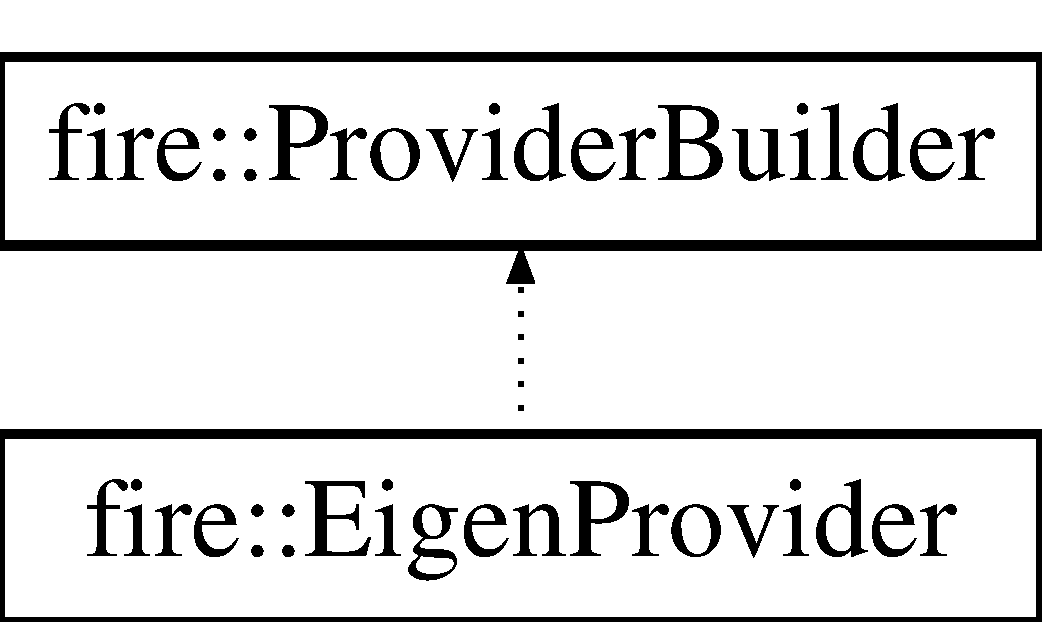
\includegraphics[height=2.000000cm]{a00834}
\end{center}
\end{figure}
\subsection*{Public Member Functions}
\begin{DoxyCompactItemize}
\item 
\mbox{\Hypertarget{a00834_ab9bfc7a0004ea10d57442f495c468b2e}\label{a00834_ab9bfc7a0004ea10d57442f495c468b2e}} 
{\footnotesize template$<$const int Rank, typename Scalar $>$ }\\\hyperlink{a00830}{Eigen\+Tensor\+Provider}$<$ Rank, Scalar $>$ {\bfseries build} ()
\end{DoxyCompactItemize}


\subsection{Detailed Description}
This class provides a mechanism for building Eigen\+Tensor\+Providers. It is used by the \hyperlink{a00838}{Tensor} class to appropriately construct a \hyperlink{a00842}{Tensor\+Provider} backed by Eigen Tensors. 

The documentation for this class was generated from the following file\+:\begin{DoxyCompactItemize}
\item 
Eigen\+Tensor\+Provider.\+hpp\end{DoxyCompactItemize}

\hypertarget{a00830}{}\section{fire\+:\+:String\+Caster$<$ T $>$ Struct Template Reference}
\label{a00830}\index{fire\+::\+String\+Caster$<$ T $>$@{fire\+::\+String\+Caster$<$ T $>$}}


{\ttfamily \#include $<$String\+Caster.\+h$>$}

\subsection*{Static Public Member Functions}
\begin{DoxyCompactItemize}
\item 
\mbox{\Hypertarget{a00830_a2f87754c1c9d5cfe64acebbaafddbbae}\label{a00830_a2f87754c1c9d5cfe64acebbaafddbbae}} 
static T {\bfseries cast} (const string \&value)
\end{DoxyCompactItemize}


\subsection{Detailed Description}
\subsubsection*{template$<$typename T$>$\newline
struct fire\+::\+String\+Caster$<$ T $>$}

Default template for casting strings properly. 

The documentation for this struct was generated from the following file\+:\begin{DoxyCompactItemize}
\item 
String\+Caster.\+h\end{DoxyCompactItemize}

\hypertarget{a00878}{}\section{C\+Simple\+Ini\+Templ$<$ S\+I\+\_\+\+C\+H\+AR, S\+I\+\_\+\+S\+T\+R\+L\+E\+SS, S\+I\+\_\+\+C\+O\+N\+V\+E\+R\+T\+ER $>$\+:\+:Entry Struct Reference}
\label{a00878}\index{C\+Simple\+Ini\+Templ$<$ S\+I\+\_\+\+C\+H\+A\+R, S\+I\+\_\+\+S\+T\+R\+L\+E\+S\+S, S\+I\+\_\+\+C\+O\+N\+V\+E\+R\+T\+E\+R $>$\+::\+Entry@{C\+Simple\+Ini\+Templ$<$ S\+I\+\_\+\+C\+H\+A\+R, S\+I\+\_\+\+S\+T\+R\+L\+E\+S\+S, S\+I\+\_\+\+C\+O\+N\+V\+E\+R\+T\+E\+R $>$\+::\+Entry}}


{\ttfamily \#include $<$Simple\+Ini.\+h$>$}

\subsection*{Classes}
\begin{DoxyCompactItemize}
\item 
struct \hyperlink{a00882}{Key\+Order}
\item 
struct \hyperlink{a00886}{Load\+Order}
\end{DoxyCompactItemize}
\subsection*{Public Member Functions}
\begin{DoxyCompactItemize}
\item 
\mbox{\Hypertarget{a00878_a20fc446e1f56f562333042a19bb57c9c}\label{a00878_a20fc446e1f56f562333042a19bb57c9c}} 
{\bfseries Entry} (const S\+I\+\_\+\+C\+H\+AR $\ast$a\+\_\+psz\+Item=N\+U\+LL, int a\+\_\+n\+Order=0)
\item 
\mbox{\Hypertarget{a00878_aaa6fc487377a2fc91dc4f0b83e572996}\label{a00878_aaa6fc487377a2fc91dc4f0b83e572996}} 
{\bfseries Entry} (const S\+I\+\_\+\+C\+H\+AR $\ast$a\+\_\+psz\+Item, const S\+I\+\_\+\+C\+H\+AR $\ast$a\+\_\+psz\+Comment, int a\+\_\+n\+Order)
\item 
\mbox{\Hypertarget{a00878_afbe8b9d3c87d5de3c6aa8d8984f011f6}\label{a00878_afbe8b9d3c87d5de3c6aa8d8984f011f6}} 
{\bfseries Entry} (const \hyperlink{a00878}{Entry} \&rhs)
\item 
\mbox{\Hypertarget{a00878_a7f4dd11cc944c140d751ae22ef6cd034}\label{a00878_a7f4dd11cc944c140d751ae22ef6cd034}} 
\hyperlink{a00878}{Entry} \& {\bfseries operator=} (const \hyperlink{a00878}{Entry} \&rhs)
\end{DoxyCompactItemize}
\subsection*{Public Attributes}
\begin{DoxyCompactItemize}
\item 
\mbox{\Hypertarget{a00878_a0f987914bf6076156c2a7c40e8e09c89}\label{a00878_a0f987914bf6076156c2a7c40e8e09c89}} 
const S\+I\+\_\+\+C\+H\+AR $\ast$ {\bfseries p\+Item}
\item 
\mbox{\Hypertarget{a00878_a84364bcded2d32c5ae4241bf197a74c4}\label{a00878_a84364bcded2d32c5ae4241bf197a74c4}} 
const S\+I\+\_\+\+C\+H\+AR $\ast$ {\bfseries p\+Comment}
\item 
\mbox{\Hypertarget{a00878_ac08ed1fec5743b35aebfa8635e1bdb5a}\label{a00878_ac08ed1fec5743b35aebfa8635e1bdb5a}} 
int {\bfseries n\+Order}
\end{DoxyCompactItemize}


\subsection{Detailed Description}
\subsubsection*{template$<$class S\+I\+\_\+\+C\+H\+AR, class S\+I\+\_\+\+S\+T\+R\+L\+E\+SS, class S\+I\+\_\+\+C\+O\+N\+V\+E\+R\+T\+ER$>$\newline
struct C\+Simple\+Ini\+Templ$<$ S\+I\+\_\+\+C\+H\+A\+R, S\+I\+\_\+\+S\+T\+R\+L\+E\+S\+S, S\+I\+\_\+\+C\+O\+N\+V\+E\+R\+T\+E\+R $>$\+::\+Entry}

key entry 

The documentation for this struct was generated from the following file\+:\begin{DoxyCompactItemize}
\item 
Simple\+Ini.\+h\end{DoxyCompactItemize}

\hypertarget{a00806}{}\section{File\+Generator Struct Reference}
\label{a00806}\index{File\+Generator@{File\+Generator}}


The documentation for this struct was generated from the following file\+:\begin{DoxyCompactItemize}
\item 
Delimited\+Text\+Parser\+Test.\+cpp\end{DoxyCompactItemize}

\hypertarget{a00894}{}\section{C\+Simple\+Ini\+Templ$<$ S\+I\+\_\+\+C\+H\+AR, S\+I\+\_\+\+S\+T\+R\+L\+E\+SS, S\+I\+\_\+\+C\+O\+N\+V\+E\+R\+T\+ER $>$\+:\+:File\+Writer Class Reference}
\label{a00894}\index{C\+Simple\+Ini\+Templ$<$ S\+I\+\_\+\+C\+H\+A\+R, S\+I\+\_\+\+S\+T\+R\+L\+E\+S\+S, S\+I\+\_\+\+C\+O\+N\+V\+E\+R\+T\+E\+R $>$\+::\+File\+Writer@{C\+Simple\+Ini\+Templ$<$ S\+I\+\_\+\+C\+H\+A\+R, S\+I\+\_\+\+S\+T\+R\+L\+E\+S\+S, S\+I\+\_\+\+C\+O\+N\+V\+E\+R\+T\+E\+R $>$\+::\+File\+Writer}}


{\ttfamily \#include $<$Simple\+Ini.\+h$>$}

Inheritance diagram for C\+Simple\+Ini\+Templ$<$ S\+I\+\_\+\+C\+H\+AR, S\+I\+\_\+\+S\+T\+R\+L\+E\+SS, S\+I\+\_\+\+C\+O\+N\+V\+E\+R\+T\+ER $>$\+:\+:File\+Writer\+:\begin{figure}[H]
\begin{center}
\leavevmode
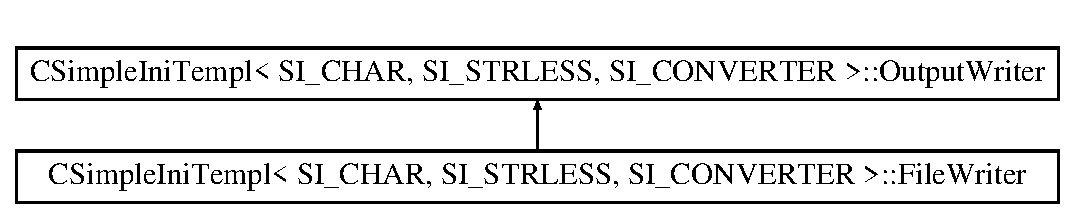
\includegraphics[height=2.000000cm]{a00894}
\end{center}
\end{figure}
\subsection*{Public Member Functions}
\begin{DoxyCompactItemize}
\item 
\mbox{\Hypertarget{a00894_aecd4d79480c9b4e70b598c10014856f8}\label{a00894_aecd4d79480c9b4e70b598c10014856f8}} 
{\bfseries File\+Writer} (F\+I\+LE $\ast$a\+\_\+file)
\item 
\mbox{\Hypertarget{a00894_ae8885b97884ef9dd5bf074bc4f011373}\label{a00894_ae8885b97884ef9dd5bf074bc4f011373}} 
void {\bfseries Write} (const char $\ast$a\+\_\+p\+Buf)
\end{DoxyCompactItemize}


\subsection{Detailed Description}
\subsubsection*{template$<$class S\+I\+\_\+\+C\+H\+AR, class S\+I\+\_\+\+S\+T\+R\+L\+E\+SS, class S\+I\+\_\+\+C\+O\+N\+V\+E\+R\+T\+ER$>$\newline
class C\+Simple\+Ini\+Templ$<$ S\+I\+\_\+\+C\+H\+A\+R, S\+I\+\_\+\+S\+T\+R\+L\+E\+S\+S, S\+I\+\_\+\+C\+O\+N\+V\+E\+R\+T\+E\+R $>$\+::\+File\+Writer}

\hyperlink{a00890}{Output\+Writer} class to write the I\+NI data to a file 

The documentation for this class was generated from the following file\+:\begin{DoxyCompactItemize}
\item 
Simple\+Ini.\+h\end{DoxyCompactItemize}

\hypertarget{a00998}{}\section{Simple\+Web\+:\+:Server$<$ H\+T\+T\+PS $>$ Class Template Reference}
\label{a00998}\index{Simple\+Web\+::\+Server$<$ H\+T\+T\+P\+S $>$@{Simple\+Web\+::\+Server$<$ H\+T\+T\+P\+S $>$}}
Inheritance diagram for Simple\+Web\+:\+:Server$<$ H\+T\+T\+PS $>$\+:\begin{figure}[H]
\begin{center}
\leavevmode
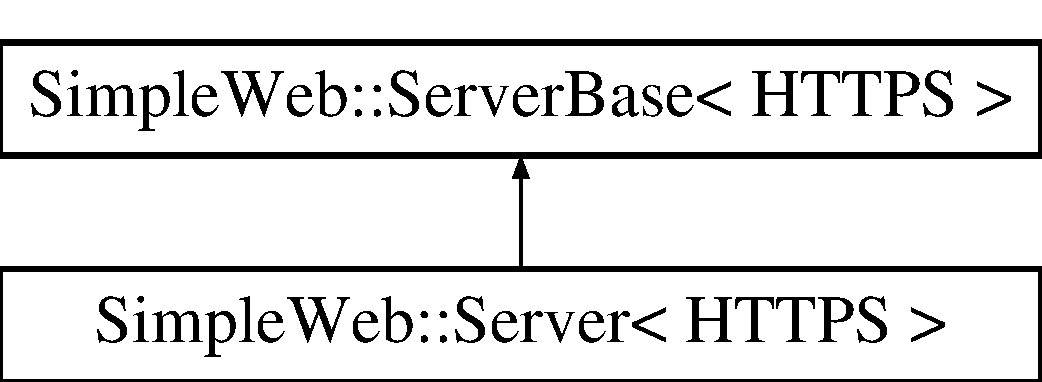
\includegraphics[height=2.000000cm]{a00998}
\end{center}
\end{figure}
\subsection*{Public Member Functions}
\begin{DoxyCompactItemize}
\item 
\mbox{\Hypertarget{a00998_a1a5530e96cd973de3dc987034ca61b54}\label{a00998_a1a5530e96cd973de3dc987034ca61b54}} 
D\+E\+P\+R\+E\+C\+A\+T\+ED {\bfseries Server} (unsigned short port, size\+\_\+t thread\+\_\+pool\+\_\+size, const std\+::string \&cert\+\_\+file, const std\+::string \&private\+\_\+key\+\_\+file, long timeout\+\_\+request=5, long timeout\+\_\+content=300, const std\+::string \&verify\+\_\+file=std\+::string())
\item 
\mbox{\Hypertarget{a00998_a15bb179287dfaa18da16b8877174e8d6}\label{a00998_a15bb179287dfaa18da16b8877174e8d6}} 
{\bfseries Server} (const std\+::string \&cert\+\_\+file, const std\+::string \&private\+\_\+key\+\_\+file, const std\+::string \&verify\+\_\+file=std\+::string())
\item 
\mbox{\Hypertarget{a00998_a6a740b3fdbbbf178f540e27942cc93fc}\label{a00998_a6a740b3fdbbbf178f540e27942cc93fc}} 
void {\bfseries start} ()
\end{DoxyCompactItemize}
\subsection*{Protected Member Functions}
\begin{DoxyCompactItemize}
\item 
\mbox{\Hypertarget{a00998_af722d2884eafafada7073feb7793c422}\label{a00998_af722d2884eafafada7073feb7793c422}} 
void {\bfseries accept} ()
\end{DoxyCompactItemize}
\subsection*{Protected Attributes}
\begin{DoxyCompactItemize}
\item 
\mbox{\Hypertarget{a00998_ade0b1e6f826fd76ba6c6253d352fd93c}\label{a00998_ade0b1e6f826fd76ba6c6253d352fd93c}} 
boost\+::asio\+::ssl\+::context {\bfseries context}
\end{DoxyCompactItemize}
\subsection*{Additional Inherited Members}


The documentation for this class was generated from the following file\+:\begin{DoxyCompactItemize}
\item 
server\+\_\+https.\+hpp\end{DoxyCompactItemize}

\hypertarget{a00762}{}\section{fire\+:\+:astrophysics\+:\+:Reaction\+Network Class Reference}
\label{a00762}\index{fire\+::astrophysics\+::\+Reaction\+Network@{fire\+::astrophysics\+::\+Reaction\+Network}}


{\ttfamily \#include $<$Reaction\+Network.\+h$>$}

\subsection*{Public Member Functions}
\begin{DoxyCompactItemize}
\item 
\mbox{\Hypertarget{a00762_a66db1b9f2e597f21bce7bcb88b1fbf8f}\label{a00762_a66db1b9f2e597f21bce7bcb88b1fbf8f}} 
double \& {\bfseries operator()} (int i)
\item 
void \hyperlink{a00762_ab4713cafb974ca41bf6a55619e9fd875}{set\+Properties} (const map$<$ string, string $>$ \&props)
\item 
void \hyperlink{a00762_aa9b4de0566ab0b0f148677d8b97e8c49}{load} ()
\item 
void \hyperlink{a00762_aa0c06237ae72e698aee9cf72d0032fd8}{build\+Flux\+Maps} ()
\item 
void \hyperlink{a00762_ac5b97490e667b011b5e2bea92e16f8b7}{compute\+Prefactors} (const double \&rho)
\item 
void \hyperlink{a00762_a3b1fee4e28576c677d7b852e91c6fa98}{compute\+Rates} (const double \&temp)
\item 
void \hyperlink{a00762_a35a05489358c8e1017bbebb75a9c0114}{compute\+Fluxes} ()
\end{DoxyCompactItemize}
\subsection*{Public Attributes}
\begin{DoxyCompactItemize}
\item 
int \hyperlink{a00762_a17ffe8399181590d59d3d339ce867709}{num\+Species}
\item 
int \hyperlink{a00762_ade8f4d9aa1524cbc45809e7943725d59}{num\+Reactions}
\item 
int \hyperlink{a00762_a91f7685b58b70eca227a098717dfe2c5}{num\+Reaction\+Groups}
\item 
double \hyperlink{a00762_ad3d95ecac758ca7efce6376904455123}{mass\+Tol}
\item 
double \hyperlink{a00762_a0bb068c675589e1ad767c1faf2165ed7}{flux\+Frac}
\item 
string \hyperlink{a00762_abcc4209749ecd64d0ab9621210536ade}{network\+File\+Name}
\item 
string \hyperlink{a00762_abb5fbb289b2e40d3b3dcb3695696e2c2}{rate\+File\+Name}
\item 
shared\+\_\+ptr$<$ vector$<$ \hyperlink{a00766}{Species} $>$ $>$ \hyperlink{a00762_ac3811889f4866a29a49ce3a8d0e80cad}{species}
\item 
shared\+\_\+ptr$<$ vector$<$ \hyperlink{a00758}{Reaction} $>$ $>$ \hyperlink{a00762_a32964b6f6a9cb312e722c1478167b7f0}{reactions}
\item 
vector$<$ double $>$ \hyperlink{a00762_af3aa4184f759b2a8babf765667aa6604}{f\+Plus\+Map}
\item 
vector$<$ double $>$ \hyperlink{a00762_a9065be108e95b1604b0d53e2080f0b57}{f\+Minus\+Map}
\item 
vector$<$ double $>$ \hyperlink{a00762_aca9928041359ecf555a63e4f58e80164}{f\+Plus\+Factors}
\item 
vector$<$ double $>$ \hyperlink{a00762_a3aff20108c80e14f9f4d526a08af49de}{f\+Minus\+Factors}
\item 
vector$<$ unsigned short $>$ \hyperlink{a00762_a6682680b1f2975fa8dc1288d3c463693}{f\+Plus\+Maximums}
\item 
vector$<$ unsigned short $>$ \hyperlink{a00762_a4ea51dc9d41bf555592f93bb237e0440}{f\+Minus\+Maximums}
\item 
\mbox{\Hypertarget{a00762_a9309d86802802f33350fbd4fd679fc2b}\label{a00762_a9309d86802802f33350fbd4fd679fc2b}} 
int {\bfseries num\+F\+Plus}
\item 
\mbox{\Hypertarget{a00762_aec06a5e98ef60a1572072c3ad3fa7722}\label{a00762_aec06a5e98ef60a1572072c3ad3fa7722}} 
int {\bfseries num\+F\+Minus}
\end{DoxyCompactItemize}


\subsection{Detailed Description}
This class collects all of the information about a thermonuclear reaction network for astrophysical systems. It includes all species and reaction information and other stateful variable.

The design of this class is not ideal because it exposes public members variables. This design is still an advancement over the original design in F\+E\+RN and is good enough for now. We\textquotesingle{}ll improve it later. 

\subsection{Member Function Documentation}
\mbox{\Hypertarget{a00762_aa0c06237ae72e698aee9cf72d0032fd8}\label{a00762_aa0c06237ae72e698aee9cf72d0032fd8}} 
\index{fire\+::astrophysics\+::\+Reaction\+Network@{fire\+::astrophysics\+::\+Reaction\+Network}!build\+Flux\+Maps@{build\+Flux\+Maps}}
\index{build\+Flux\+Maps@{build\+Flux\+Maps}!fire\+::astrophysics\+::\+Reaction\+Network@{fire\+::astrophysics\+::\+Reaction\+Network}}
\subsubsection{\texorpdfstring{build\+Flux\+Maps()}{buildFluxMaps()}}
{\footnotesize\ttfamily void fire\+::astrophysics\+::\+Reaction\+Network\+::build\+Flux\+Maps (\begin{DoxyParamCaption}{ }\end{DoxyParamCaption})\hspace{0.3cm}{\ttfamily [inline]}}

This operation builds the \char`\"{}flux maps\char`\"{} that map the contributions of each reaction for each species in the network.

This function was originally written as part of the F\+E\+RN code and desperately needs to be refactored. It is has been adapted to use the \hyperlink{a00766}{Species} and \hyperlink{a00758}{Reaction} classes in Fire, but still contains a number of old constructs that have poor performance implications. Likewise, it lacks a sophisticated view of data structures that could greatly increase its speed. It is fine for now because ultimately the formation of the flux maps and numerical prefactors on the R\+HS take up an extremely small amount of computational time compared to the rest of the integration since they are only computed once on initialization of the network. \mbox{\Hypertarget{a00762_a35a05489358c8e1017bbebb75a9c0114}\label{a00762_a35a05489358c8e1017bbebb75a9c0114}} 
\index{fire\+::astrophysics\+::\+Reaction\+Network@{fire\+::astrophysics\+::\+Reaction\+Network}!compute\+Fluxes@{compute\+Fluxes}}
\index{compute\+Fluxes@{compute\+Fluxes}!fire\+::astrophysics\+::\+Reaction\+Network@{fire\+::astrophysics\+::\+Reaction\+Network}}
\subsubsection{\texorpdfstring{compute\+Fluxes()}{computeFluxes()}}
{\footnotesize\ttfamily void fire\+::astrophysics\+::\+Reaction\+Network\+::compute\+Fluxes (\begin{DoxyParamCaption}{ }\end{DoxyParamCaption})\hspace{0.3cm}{\ttfamily [inline]}}

This operation computes the fluxes for the species in the network under the given conditions. The fluxes are stored in the flux member variable on the species itself. \mbox{\Hypertarget{a00762_ac5b97490e667b011b5e2bea92e16f8b7}\label{a00762_ac5b97490e667b011b5e2bea92e16f8b7}} 
\index{fire\+::astrophysics\+::\+Reaction\+Network@{fire\+::astrophysics\+::\+Reaction\+Network}!compute\+Prefactors@{compute\+Prefactors}}
\index{compute\+Prefactors@{compute\+Prefactors}!fire\+::astrophysics\+::\+Reaction\+Network@{fire\+::astrophysics\+::\+Reaction\+Network}}
\subsubsection{\texorpdfstring{compute\+Prefactors()}{computePrefactors()}}
{\footnotesize\ttfamily void fire\+::astrophysics\+::\+Reaction\+Network\+::compute\+Prefactors (\begin{DoxyParamCaption}\item[{const double \&}]{rho }\end{DoxyParamCaption})\hspace{0.3cm}{\ttfamily [inline]}}

This function computes the prefactors for the reaction rates. It is primarily a convenience function for configuring the reactions. The prefactors are stored in the reactions themselves. 
\begin{DoxyParams}{Parameters}
{\em rho} & the current density in units of g/m$^\wedge$3. \\
\hline
\end{DoxyParams}
\mbox{\Hypertarget{a00762_a3b1fee4e28576c677d7b852e91c6fa98}\label{a00762_a3b1fee4e28576c677d7b852e91c6fa98}} 
\index{fire\+::astrophysics\+::\+Reaction\+Network@{fire\+::astrophysics\+::\+Reaction\+Network}!compute\+Rates@{compute\+Rates}}
\index{compute\+Rates@{compute\+Rates}!fire\+::astrophysics\+::\+Reaction\+Network@{fire\+::astrophysics\+::\+Reaction\+Network}}
\subsubsection{\texorpdfstring{compute\+Rates()}{computeRates()}}
{\footnotesize\ttfamily void fire\+::astrophysics\+::\+Reaction\+Network\+::compute\+Rates (\begin{DoxyParamCaption}\item[{const double \&}]{temp }\end{DoxyParamCaption})\hspace{0.3cm}{\ttfamily [inline]}}

This function computers the reaction rates. It is primarily a convenience function for configuring the reactions. The rates are stored in the rate member variable on the reaction itself. 
\begin{DoxyParams}{Parameters}
{\em temp} & the current temperature in units of 10$^\wedge$9 Kelvin. \\
\hline
\end{DoxyParams}
\mbox{\Hypertarget{a00762_aa9b4de0566ab0b0f148677d8b97e8c49}\label{a00762_aa9b4de0566ab0b0f148677d8b97e8c49}} 
\index{fire\+::astrophysics\+::\+Reaction\+Network@{fire\+::astrophysics\+::\+Reaction\+Network}!load@{load}}
\index{load@{load}!fire\+::astrophysics\+::\+Reaction\+Network@{fire\+::astrophysics\+::\+Reaction\+Network}}
\subsubsection{\texorpdfstring{load()}{load()}}
{\footnotesize\ttfamily void fire\+::astrophysics\+::\+Reaction\+Network\+::load (\begin{DoxyParamCaption}{ }\end{DoxyParamCaption})\hspace{0.3cm}{\ttfamily [inline]}}

This operations directs the Network to load the species and reactions from the files provided in the properties list. \mbox{\Hypertarget{a00762_ab4713cafb974ca41bf6a55619e9fd875}\label{a00762_ab4713cafb974ca41bf6a55619e9fd875}} 
\index{fire\+::astrophysics\+::\+Reaction\+Network@{fire\+::astrophysics\+::\+Reaction\+Network}!set\+Properties@{set\+Properties}}
\index{set\+Properties@{set\+Properties}!fire\+::astrophysics\+::\+Reaction\+Network@{fire\+::astrophysics\+::\+Reaction\+Network}}
\subsubsection{\texorpdfstring{set\+Properties()}{setProperties()}}
{\footnotesize\ttfamily void fire\+::astrophysics\+::\+Reaction\+Network\+::set\+Properties (\begin{DoxyParamCaption}\item[{const map$<$ string, string $>$ \&}]{props }\end{DoxyParamCaption})\hspace{0.3cm}{\ttfamily [inline]}}

This operation sets the properties of the network from a map. It is designed to work with property blocks pulled from I\+NI files. It expects the following keys to have values in the map and accepts the default if they do not\+: num\+Species num\+Reactions num\+Reaction\+Groups mass\+Tol flux\+Frac network\+File rate\+File 
\begin{DoxyParams}{Parameters}
{\em props} & the property map \\
\hline
\end{DoxyParams}


\subsection{Member Data Documentation}
\mbox{\Hypertarget{a00762_a0bb068c675589e1ad767c1faf2165ed7}\label{a00762_a0bb068c675589e1ad767c1faf2165ed7}} 
\index{fire\+::astrophysics\+::\+Reaction\+Network@{fire\+::astrophysics\+::\+Reaction\+Network}!flux\+Frac@{flux\+Frac}}
\index{flux\+Frac@{flux\+Frac}!fire\+::astrophysics\+::\+Reaction\+Network@{fire\+::astrophysics\+::\+Reaction\+Network}}
\subsubsection{\texorpdfstring{flux\+Frac}{fluxFrac}}
{\footnotesize\ttfamily double fire\+::astrophysics\+::\+Reaction\+Network\+::flux\+Frac}

A tunable parameter to limit the integration step size based solely on the flux \mbox{\Hypertarget{a00762_a3aff20108c80e14f9f4d526a08af49de}\label{a00762_a3aff20108c80e14f9f4d526a08af49de}} 
\index{fire\+::astrophysics\+::\+Reaction\+Network@{fire\+::astrophysics\+::\+Reaction\+Network}!f\+Minus\+Factors@{f\+Minus\+Factors}}
\index{f\+Minus\+Factors@{f\+Minus\+Factors}!fire\+::astrophysics\+::\+Reaction\+Network@{fire\+::astrophysics\+::\+Reaction\+Network}}
\subsubsection{\texorpdfstring{f\+Minus\+Factors}{fMinusFactors}}
{\footnotesize\ttfamily vector$<$double$>$ fire\+::astrophysics\+::\+Reaction\+Network\+::f\+Minus\+Factors}

The array of size num\+Species$\ast$num\+Reactions that contains the serialized set of numerical factors due to detracting fluxes. \mbox{\Hypertarget{a00762_a9065be108e95b1604b0d53e2080f0b57}\label{a00762_a9065be108e95b1604b0d53e2080f0b57}} 
\index{fire\+::astrophysics\+::\+Reaction\+Network@{fire\+::astrophysics\+::\+Reaction\+Network}!f\+Minus\+Map@{f\+Minus\+Map}}
\index{f\+Minus\+Map@{f\+Minus\+Map}!fire\+::astrophysics\+::\+Reaction\+Network@{fire\+::astrophysics\+::\+Reaction\+Network}}
\subsubsection{\texorpdfstring{f\+Minus\+Map}{fMinusMap}}
{\footnotesize\ttfamily vector$<$double$>$ fire\+::astrophysics\+::\+Reaction\+Network\+::f\+Minus\+Map}

The array of size num\+Species$\ast$num\+Reactions that contains the serialized map of detracting fluxes for each reaction for each species. \mbox{\Hypertarget{a00762_a4ea51dc9d41bf555592f93bb237e0440}\label{a00762_a4ea51dc9d41bf555592f93bb237e0440}} 
\index{fire\+::astrophysics\+::\+Reaction\+Network@{fire\+::astrophysics\+::\+Reaction\+Network}!f\+Minus\+Maximums@{f\+Minus\+Maximums}}
\index{f\+Minus\+Maximums@{f\+Minus\+Maximums}!fire\+::astrophysics\+::\+Reaction\+Network@{fire\+::astrophysics\+::\+Reaction\+Network}}
\subsubsection{\texorpdfstring{f\+Minus\+Maximums}{fMinusMaximums}}
{\footnotesize\ttfamily vector$<$unsigned short$>$ fire\+::astrophysics\+::\+Reaction\+Network\+::f\+Minus\+Maximums}

The array of maximum detracting flux values for each species in the network. (Size = num\+Species) \mbox{\Hypertarget{a00762_aca9928041359ecf555a63e4f58e80164}\label{a00762_aca9928041359ecf555a63e4f58e80164}} 
\index{fire\+::astrophysics\+::\+Reaction\+Network@{fire\+::astrophysics\+::\+Reaction\+Network}!f\+Plus\+Factors@{f\+Plus\+Factors}}
\index{f\+Plus\+Factors@{f\+Plus\+Factors}!fire\+::astrophysics\+::\+Reaction\+Network@{fire\+::astrophysics\+::\+Reaction\+Network}}
\subsubsection{\texorpdfstring{f\+Plus\+Factors}{fPlusFactors}}
{\footnotesize\ttfamily vector$<$double$>$ fire\+::astrophysics\+::\+Reaction\+Network\+::f\+Plus\+Factors}

The array of size num\+Species$\ast$num\+Reactions that contains the serialized set of numerical factors due to contributing fluxes. \mbox{\Hypertarget{a00762_af3aa4184f759b2a8babf765667aa6604}\label{a00762_af3aa4184f759b2a8babf765667aa6604}} 
\index{fire\+::astrophysics\+::\+Reaction\+Network@{fire\+::astrophysics\+::\+Reaction\+Network}!f\+Plus\+Map@{f\+Plus\+Map}}
\index{f\+Plus\+Map@{f\+Plus\+Map}!fire\+::astrophysics\+::\+Reaction\+Network@{fire\+::astrophysics\+::\+Reaction\+Network}}
\subsubsection{\texorpdfstring{f\+Plus\+Map}{fPlusMap}}
{\footnotesize\ttfamily vector$<$double$>$ fire\+::astrophysics\+::\+Reaction\+Network\+::f\+Plus\+Map}

The array of size num\+Species$\ast$num\+Reactions that contains the serialized map of contributing fluxes for each reaction for each species. \mbox{\Hypertarget{a00762_a6682680b1f2975fa8dc1288d3c463693}\label{a00762_a6682680b1f2975fa8dc1288d3c463693}} 
\index{fire\+::astrophysics\+::\+Reaction\+Network@{fire\+::astrophysics\+::\+Reaction\+Network}!f\+Plus\+Maximums@{f\+Plus\+Maximums}}
\index{f\+Plus\+Maximums@{f\+Plus\+Maximums}!fire\+::astrophysics\+::\+Reaction\+Network@{fire\+::astrophysics\+::\+Reaction\+Network}}
\subsubsection{\texorpdfstring{f\+Plus\+Maximums}{fPlusMaximums}}
{\footnotesize\ttfamily vector$<$unsigned short$>$ fire\+::astrophysics\+::\+Reaction\+Network\+::f\+Plus\+Maximums}

The array of maximum contributing flux values for each species in the network. (Size = num\+Species) \mbox{\Hypertarget{a00762_ad3d95ecac758ca7efce6376904455123}\label{a00762_ad3d95ecac758ca7efce6376904455123}} 
\index{fire\+::astrophysics\+::\+Reaction\+Network@{fire\+::astrophysics\+::\+Reaction\+Network}!mass\+Tol@{mass\+Tol}}
\index{mass\+Tol@{mass\+Tol}!fire\+::astrophysics\+::\+Reaction\+Network@{fire\+::astrophysics\+::\+Reaction\+Network}}
\subsubsection{\texorpdfstring{mass\+Tol}{massTol}}
{\footnotesize\ttfamily double fire\+::astrophysics\+::\+Reaction\+Network\+::mass\+Tol}

The mass tolerance for integration in the network \mbox{\Hypertarget{a00762_abcc4209749ecd64d0ab9621210536ade}\label{a00762_abcc4209749ecd64d0ab9621210536ade}} 
\index{fire\+::astrophysics\+::\+Reaction\+Network@{fire\+::astrophysics\+::\+Reaction\+Network}!network\+File\+Name@{network\+File\+Name}}
\index{network\+File\+Name@{network\+File\+Name}!fire\+::astrophysics\+::\+Reaction\+Network@{fire\+::astrophysics\+::\+Reaction\+Network}}
\subsubsection{\texorpdfstring{network\+File\+Name}{networkFileName}}
{\footnotesize\ttfamily string fire\+::astrophysics\+::\+Reaction\+Network\+::network\+File\+Name}

The name of file that contains the species present in the network. \mbox{\Hypertarget{a00762_a91f7685b58b70eca227a098717dfe2c5}\label{a00762_a91f7685b58b70eca227a098717dfe2c5}} 
\index{fire\+::astrophysics\+::\+Reaction\+Network@{fire\+::astrophysics\+::\+Reaction\+Network}!num\+Reaction\+Groups@{num\+Reaction\+Groups}}
\index{num\+Reaction\+Groups@{num\+Reaction\+Groups}!fire\+::astrophysics\+::\+Reaction\+Network@{fire\+::astrophysics\+::\+Reaction\+Network}}
\subsubsection{\texorpdfstring{num\+Reaction\+Groups}{numReactionGroups}}
{\footnotesize\ttfamily int fire\+::astrophysics\+::\+Reaction\+Network\+::num\+Reaction\+Groups}

The number of reaction groups in the network \mbox{\Hypertarget{a00762_ade8f4d9aa1524cbc45809e7943725d59}\label{a00762_ade8f4d9aa1524cbc45809e7943725d59}} 
\index{fire\+::astrophysics\+::\+Reaction\+Network@{fire\+::astrophysics\+::\+Reaction\+Network}!num\+Reactions@{num\+Reactions}}
\index{num\+Reactions@{num\+Reactions}!fire\+::astrophysics\+::\+Reaction\+Network@{fire\+::astrophysics\+::\+Reaction\+Network}}
\subsubsection{\texorpdfstring{num\+Reactions}{numReactions}}
{\footnotesize\ttfamily int fire\+::astrophysics\+::\+Reaction\+Network\+::num\+Reactions}

The number of reactions between the species in the network \mbox{\Hypertarget{a00762_a17ffe8399181590d59d3d339ce867709}\label{a00762_a17ffe8399181590d59d3d339ce867709}} 
\index{fire\+::astrophysics\+::\+Reaction\+Network@{fire\+::astrophysics\+::\+Reaction\+Network}!num\+Species@{num\+Species}}
\index{num\+Species@{num\+Species}!fire\+::astrophysics\+::\+Reaction\+Network@{fire\+::astrophysics\+::\+Reaction\+Network}}
\subsubsection{\texorpdfstring{num\+Species}{numSpecies}}
{\footnotesize\ttfamily int fire\+::astrophysics\+::\+Reaction\+Network\+::num\+Species}

The number of species in the network \mbox{\Hypertarget{a00762_abb5fbb289b2e40d3b3dcb3695696e2c2}\label{a00762_abb5fbb289b2e40d3b3dcb3695696e2c2}} 
\index{fire\+::astrophysics\+::\+Reaction\+Network@{fire\+::astrophysics\+::\+Reaction\+Network}!rate\+File\+Name@{rate\+File\+Name}}
\index{rate\+File\+Name@{rate\+File\+Name}!fire\+::astrophysics\+::\+Reaction\+Network@{fire\+::astrophysics\+::\+Reaction\+Network}}
\subsubsection{\texorpdfstring{rate\+File\+Name}{rateFileName}}
{\footnotesize\ttfamily string fire\+::astrophysics\+::\+Reaction\+Network\+::rate\+File\+Name}

The name of the file that contains the reaction data for the network. \mbox{\Hypertarget{a00762_a32964b6f6a9cb312e722c1478167b7f0}\label{a00762_a32964b6f6a9cb312e722c1478167b7f0}} 
\index{fire\+::astrophysics\+::\+Reaction\+Network@{fire\+::astrophysics\+::\+Reaction\+Network}!reactions@{reactions}}
\index{reactions@{reactions}!fire\+::astrophysics\+::\+Reaction\+Network@{fire\+::astrophysics\+::\+Reaction\+Network}}
\subsubsection{\texorpdfstring{reactions}{reactions}}
{\footnotesize\ttfamily shared\+\_\+ptr$<$vector$<$\hyperlink{a00758}{Reaction}$>$ $>$ fire\+::astrophysics\+::\+Reaction\+Network\+::reactions}

This is the list of reactions in the network. \mbox{\Hypertarget{a00762_ac3811889f4866a29a49ce3a8d0e80cad}\label{a00762_ac3811889f4866a29a49ce3a8d0e80cad}} 
\index{fire\+::astrophysics\+::\+Reaction\+Network@{fire\+::astrophysics\+::\+Reaction\+Network}!species@{species}}
\index{species@{species}!fire\+::astrophysics\+::\+Reaction\+Network@{fire\+::astrophysics\+::\+Reaction\+Network}}
\subsubsection{\texorpdfstring{species}{species}}
{\footnotesize\ttfamily shared\+\_\+ptr$<$vector$<$\hyperlink{a00766}{Species}$>$ $>$ fire\+::astrophysics\+::\+Reaction\+Network\+::species}

This is the list of species in the network. 

The documentation for this class was generated from the following file\+:\begin{DoxyCompactItemize}
\item 
Reaction\+Network.\+h\end{DoxyCompactItemize}

\hypertarget{a01002}{}\section{fire\+:\+:util\+:\+:Asio\+Networking\+Tool$<$ P\+R\+O\+T\+O\+C\+OL $>$ Class Template Reference}
\label{a01002}\index{fire\+::util\+::\+Asio\+Networking\+Tool$<$ P\+R\+O\+T\+O\+C\+O\+L $>$@{fire\+::util\+::\+Asio\+Networking\+Tool$<$ P\+R\+O\+T\+O\+C\+O\+L $>$}}


{\ttfamily \#include $<$Asio\+Networking\+Tool.\+hpp$>$}

Inheritance diagram for fire\+:\+:util\+:\+:Asio\+Networking\+Tool$<$ P\+R\+O\+T\+O\+C\+OL $>$\+:\begin{figure}[H]
\begin{center}
\leavevmode
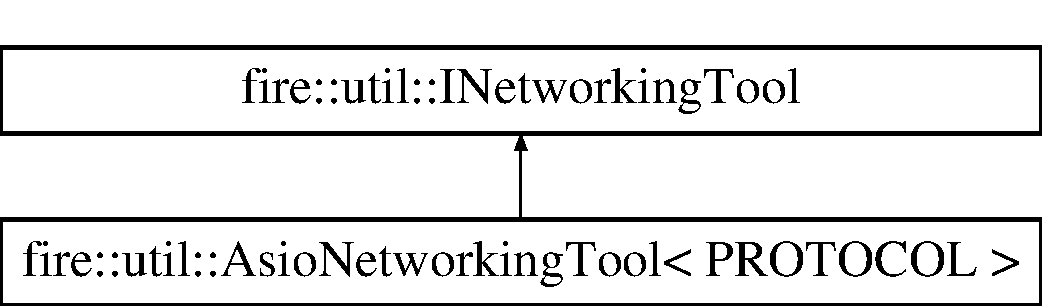
\includegraphics[height=2.000000cm]{a01002}
\end{center}
\end{figure}
\subsection*{Public Member Functions}
\begin{DoxyCompactItemize}
\item 
\hyperlink{a01002_a5edd72ce9937e052a82e7564500b3861}{Asio\+Networking\+Tool} (std\+::string host, int p)
\item 
\mbox{\Hypertarget{a01002_a5826de4a9e051ec854ad7be3a48ac86d}\label{a01002_a5826de4a9e051ec854ad7be3a48ac86d}} 
{\bfseries Asio\+Networking\+Tool} (std\+::string host\+\_\+and\+\_\+port, bool verify\+Cert=true, const std\+::string \&cert\+\_\+file=std\+::string(), const std\+::string \&private\+\_\+key\+\_\+file=std\+::string(), const std\+::string \&verify\+\_\+file=std\+::string())
\item 
virtual \hyperlink{a01002_afc51c728e1bd136b6729ac892df490ab}{$\sim$\+Asio\+Networking\+Tool} ()
\item 
virtual \hyperlink{a01006}{Http\+Response} \hyperlink{a01002_a42609f768f245acf0867889e920c5d49}{get} (const std\+::string \&relative\+Path, const std\+::map$<$ std\+::string, std\+::string $>$ \&header=std\+::map$<$ std\+::string, std\+::string $>$())
\item 
virtual \hyperlink{a01006}{Http\+Response} \hyperlink{a01002_a2ac524ceef89fceb928cf74420bf90a5}{post} (const std\+::string \&relative\+Path, const std\+::string \&message, const std\+::map$<$ std\+::string, std\+::string $>$ \&header=std\+::map$<$ std\+::string, std\+::string $>$())
\end{DoxyCompactItemize}
\subsection*{Protected Attributes}
\begin{DoxyCompactItemize}
\item 
std\+::shared\+\_\+ptr$<$ \hyperlink{a00942}{Web\+Client} $>$ \hyperlink{a01002_a57412dca950e86b857ee4795a9b6517e}{client}
\item 
\mbox{\Hypertarget{a01002_a613f571530390cf1d05538c658c13b9e}\label{a01002_a613f571530390cf1d05538c658c13b9e}} 
std\+::shared\+\_\+ptr$<$ Response\+Type $>$ {\bfseries response}
\end{DoxyCompactItemize}


\subsection{Detailed Description}
\subsubsection*{template$<$typename P\+R\+O\+T\+O\+C\+OL$>$\newline
class fire\+::util\+::\+Asio\+Networking\+Tool$<$ P\+R\+O\+T\+O\+C\+O\+L $>$}

The Asio\+Networkign\+Tool is a realization of the \hyperlink{a01010}{I\+Networking\+Tool} interface that uses the B\+O\+O\+ST Asio library to post/get http requests. 

\subsection{Constructor \& Destructor Documentation}
\mbox{\Hypertarget{a01002_a5edd72ce9937e052a82e7564500b3861}\label{a01002_a5edd72ce9937e052a82e7564500b3861}} 
\index{fire\+::util\+::\+Asio\+Networking\+Tool@{fire\+::util\+::\+Asio\+Networking\+Tool}!Asio\+Networking\+Tool@{Asio\+Networking\+Tool}}
\index{Asio\+Networking\+Tool@{Asio\+Networking\+Tool}!fire\+::util\+::\+Asio\+Networking\+Tool@{fire\+::util\+::\+Asio\+Networking\+Tool}}
\subsubsection{\texorpdfstring{Asio\+Networking\+Tool()}{AsioNetworkingTool()}}
{\footnotesize\ttfamily template$<$typename P\+R\+O\+T\+O\+C\+OL $>$ \\
\hyperlink{a01002}{fire\+::util\+::\+Asio\+Networking\+Tool}$<$ P\+R\+O\+T\+O\+C\+OL $>$\+::\hyperlink{a01002}{Asio\+Networking\+Tool} (\begin{DoxyParamCaption}\item[{std\+::string}]{host,  }\item[{int}]{p }\end{DoxyParamCaption})\hspace{0.3cm}{\ttfamily [inline]}}

The constructor \mbox{\Hypertarget{a01002_afc51c728e1bd136b6729ac892df490ab}\label{a01002_afc51c728e1bd136b6729ac892df490ab}} 
\index{fire\+::util\+::\+Asio\+Networking\+Tool@{fire\+::util\+::\+Asio\+Networking\+Tool}!````~Asio\+Networking\+Tool@{$\sim$\+Asio\+Networking\+Tool}}
\index{````~Asio\+Networking\+Tool@{$\sim$\+Asio\+Networking\+Tool}!fire\+::util\+::\+Asio\+Networking\+Tool@{fire\+::util\+::\+Asio\+Networking\+Tool}}
\subsubsection{\texorpdfstring{$\sim$\+Asio\+Networking\+Tool()}{~AsioNetworkingTool()}}
{\footnotesize\ttfamily template$<$typename P\+R\+O\+T\+O\+C\+OL $>$ \\
virtual \hyperlink{a01002}{fire\+::util\+::\+Asio\+Networking\+Tool}$<$ P\+R\+O\+T\+O\+C\+OL $>$\+::$\sim$\hyperlink{a01002}{Asio\+Networking\+Tool} (\begin{DoxyParamCaption}{ }\end{DoxyParamCaption})\hspace{0.3cm}{\ttfamily [inline]}, {\ttfamily [virtual]}}

The destructor 

\subsection{Member Function Documentation}
\mbox{\Hypertarget{a01002_a42609f768f245acf0867889e920c5d49}\label{a01002_a42609f768f245acf0867889e920c5d49}} 
\index{fire\+::util\+::\+Asio\+Networking\+Tool@{fire\+::util\+::\+Asio\+Networking\+Tool}!get@{get}}
\index{get@{get}!fire\+::util\+::\+Asio\+Networking\+Tool@{fire\+::util\+::\+Asio\+Networking\+Tool}}
\subsubsection{\texorpdfstring{get()}{get()}}
{\footnotesize\ttfamily template$<$typename P\+R\+O\+T\+O\+C\+OL $>$ \\
virtual \hyperlink{a01006}{Http\+Response} \hyperlink{a01002}{fire\+::util\+::\+Asio\+Networking\+Tool}$<$ P\+R\+O\+T\+O\+C\+OL $>$\+::get (\begin{DoxyParamCaption}\item[{const std\+::string \&}]{relative\+Path,  }\item[{const std\+::map$<$ std\+::string, std\+::string $>$ \&}]{header = {\ttfamily std\+:\+:map$<$~std\+:\+:string,~std\+:\+:string$>$()} }\end{DoxyParamCaption})\hspace{0.3cm}{\ttfamily [inline]}, {\ttfamily [virtual]}}

Return the last received status code.

\begin{DoxyReturn}{Returns}
code The status code as a string Issue an H\+T\+TP G\+ET Command at the given relative path. Clients can provide a map of header key values to modify the G\+ET request.
\end{DoxyReturn}

\begin{DoxyParams}{Parameters}
{\em relative\+Path} & The path relative to the hostname/port provided to this Networking\+Tool \\
\hline
\end{DoxyParams}
\begin{DoxyReturn}{Returns}
The contents at the U\+RL or an error message if one took place. 
\end{DoxyReturn}


Implements \hyperlink{a01010_a44b81ebf8421f0e32ed99b5e372ef007}{fire\+::util\+::\+I\+Networking\+Tool}.

\mbox{\Hypertarget{a01002_a2ac524ceef89fceb928cf74420bf90a5}\label{a01002_a2ac524ceef89fceb928cf74420bf90a5}} 
\index{fire\+::util\+::\+Asio\+Networking\+Tool@{fire\+::util\+::\+Asio\+Networking\+Tool}!post@{post}}
\index{post@{post}!fire\+::util\+::\+Asio\+Networking\+Tool@{fire\+::util\+::\+Asio\+Networking\+Tool}}
\subsubsection{\texorpdfstring{post()}{post()}}
{\footnotesize\ttfamily template$<$typename P\+R\+O\+T\+O\+C\+OL $>$ \\
virtual \hyperlink{a01006}{Http\+Response} \hyperlink{a01002}{fire\+::util\+::\+Asio\+Networking\+Tool}$<$ P\+R\+O\+T\+O\+C\+OL $>$\+::post (\begin{DoxyParamCaption}\item[{const std\+::string \&}]{relative\+Path,  }\item[{const std\+::string \&}]{message,  }\item[{const std\+::map$<$ std\+::string, std\+::string $>$ \&}]{header = {\ttfamily std\+:\+:map$<$~std\+:\+:string,~std\+:\+:string$>$()} }\end{DoxyParamCaption})\hspace{0.3cm}{\ttfamily [inline]}, {\ttfamily [virtual]}}

Issue an H\+T\+TP Post command at the given relative path with the provided message. Clients can provide a map of header key values to modify the P\+O\+ST request.


\begin{DoxyParams}{Parameters}
{\em relative\+Path} & The path relative to the hostname/port provided to this Networking\+Tool \\
\hline
{\em message} & The message to post \\
\hline
{\em header} & The map of additional H\+T\+TP P\+O\+ST header information \\
\hline
\end{DoxyParams}
\begin{DoxyReturn}{Returns}
success Boolean indicating if post was successful 
\end{DoxyReturn}


Implements \hyperlink{a01010_ad6ff0e352d78f17a6f6184d1b80e0c94}{fire\+::util\+::\+I\+Networking\+Tool}.



\subsection{Member Data Documentation}
\mbox{\Hypertarget{a01002_a57412dca950e86b857ee4795a9b6517e}\label{a01002_a57412dca950e86b857ee4795a9b6517e}} 
\index{fire\+::util\+::\+Asio\+Networking\+Tool@{fire\+::util\+::\+Asio\+Networking\+Tool}!client@{client}}
\index{client@{client}!fire\+::util\+::\+Asio\+Networking\+Tool@{fire\+::util\+::\+Asio\+Networking\+Tool}}
\subsubsection{\texorpdfstring{client}{client}}
{\footnotesize\ttfamily template$<$typename P\+R\+O\+T\+O\+C\+OL $>$ \\
std\+::shared\+\_\+ptr$<$\hyperlink{a00942}{Web\+Client}$>$ \hyperlink{a01002}{fire\+::util\+::\+Asio\+Networking\+Tool}$<$ P\+R\+O\+T\+O\+C\+OL $>$\+::client\hspace{0.3cm}{\ttfamily [protected]}}

Reference to the asio client we will use 

The documentation for this class was generated from the following file\+:\begin{DoxyCompactItemize}
\item 
Asio\+Networking\+Tool.\+hpp\end{DoxyCompactItemize}

\hypertarget{a00766}{}\section{fire\+:\+:I\+N\+I\+Property\+Parser Class Reference}
\label{a00766}\index{fire\+::\+I\+N\+I\+Property\+Parser@{fire\+::\+I\+N\+I\+Property\+Parser}}


{\ttfamily \#include $<$I\+N\+I\+Property\+Parser.\+h$>$}

Inheritance diagram for fire\+:\+:I\+N\+I\+Property\+Parser\+:\begin{figure}[H]
\begin{center}
\leavevmode
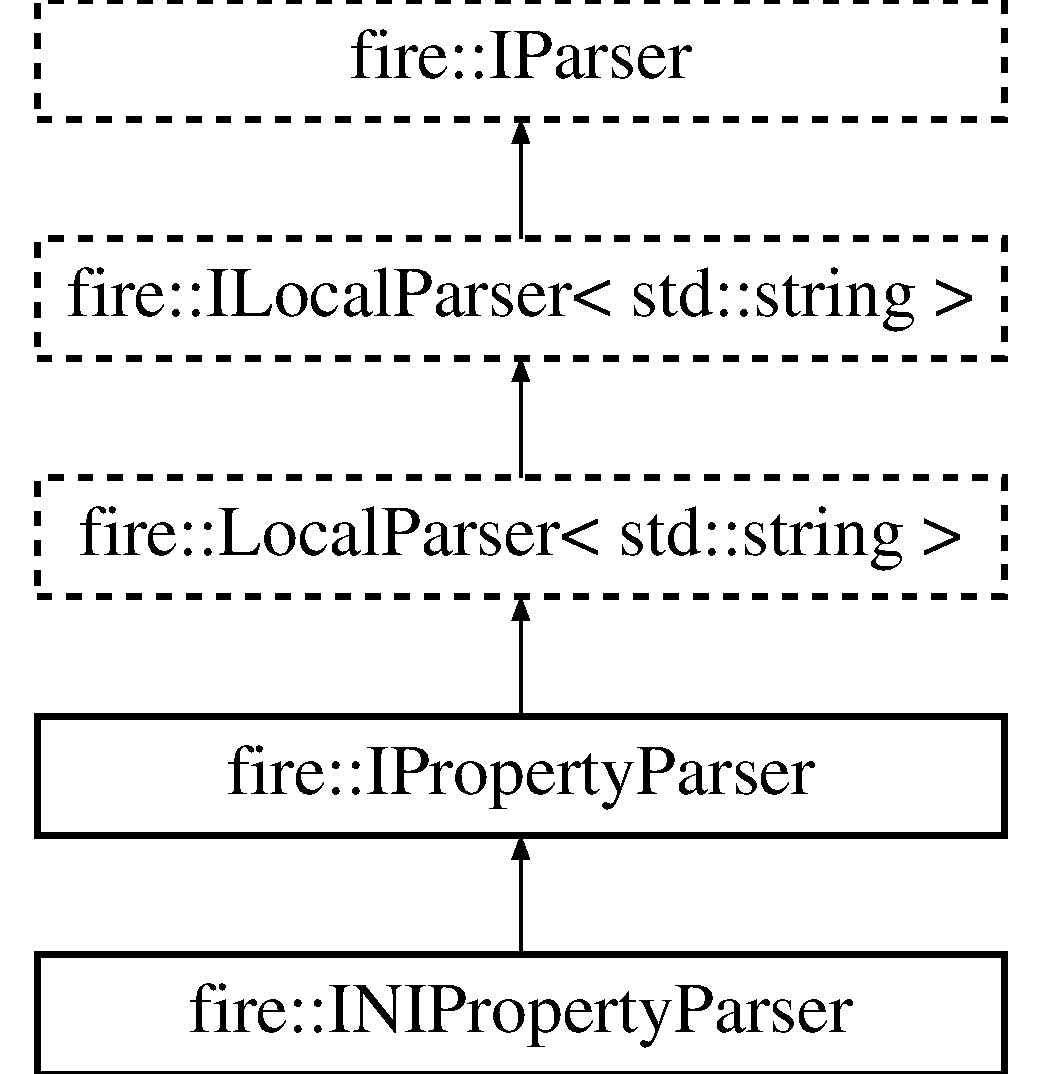
\includegraphics[height=5.000000cm]{a00766}
\end{center}
\end{figure}
\subsection*{Public Member Functions}
\begin{DoxyCompactItemize}
\item 
virtual void \hyperlink{a00766_a06793909bc707a69d0c5772b14bc946d}{set\+Source} (const std\+::string \&source)
\item 
virtual const std\+::string \& \hyperlink{a00766_ad02c9a530f20a706d7bb2554813e8d3a}{get\+Source} ()
\item 
virtual void \hyperlink{a00766_a31b6bad01e65ed4bb5f1ba297616c641}{parse} ()
\item 
virtual const std\+::vector$<$ std\+::string $>$ \& \hyperlink{a00766_aed0f1f47111794659564dcddb4d25bc6}{get\+Property\+Block\+Names} ()
\item 
virtual const std\+::map$<$ std\+::string, std\+::string $>$ \& \hyperlink{a00766_a3591312590a66659ebd377cdde9ab9ad}{get\+Property\+Block} (const std\+::string \&name)
\end{DoxyCompactItemize}
\subsection*{Additional Inherited Members}


\subsection{Detailed Description}
This class implements \hyperlink{a00774}{I\+Property\+Parser} to provide a local, file-\/based, serially executed I\+NI parser.

\hyperlink{a00762_a091d5cf56bf8f407854ef87f460b2958}{is\+File()} always returns true. \hyperlink{a00762_a770acae6e216de3a9c7140a12de25d58}{is\+Local()} always returns true. \hyperlink{a00762_ad46898c516adcce38acbb4800dc9777b}{is\+Parallel()} always returns false.

This implementation is backed by Simple\+I\+NI, one of Fire\textquotesingle{}s dependencies, so it supports whatever Simple\+I\+NI supports.

The source must be a file on the local filesystem. 

\subsection{Member Function Documentation}
\mbox{\Hypertarget{a00766_a3591312590a66659ebd377cdde9ab9ad}\label{a00766_a3591312590a66659ebd377cdde9ab9ad}} 
\index{fire\+::\+I\+N\+I\+Property\+Parser@{fire\+::\+I\+N\+I\+Property\+Parser}!get\+Property\+Block@{get\+Property\+Block}}
\index{get\+Property\+Block@{get\+Property\+Block}!fire\+::\+I\+N\+I\+Property\+Parser@{fire\+::\+I\+N\+I\+Property\+Parser}}
\subsubsection{\texorpdfstring{get\+Property\+Block()}{getPropertyBlock()}}
{\footnotesize\ttfamily virtual const std\+::map$<$std\+::string, std\+::string$>$\& fire\+::\+I\+N\+I\+Property\+Parser\+::get\+Property\+Block (\begin{DoxyParamCaption}\item[{const std\+::string \&}]{name }\end{DoxyParamCaption})\hspace{0.3cm}{\ttfamily [inline]}, {\ttfamily [virtual]}}

This operation returns the property block with the given name. 
\begin{DoxyParams}{Parameters}
{\em name} & the block name \\
\hline
\end{DoxyParams}
\begin{DoxyReturn}{Returns}
the property block with the given name 
\end{DoxyReturn}


Implements \hyperlink{a00774_a34201371cb36dd09e96a66242ececb86}{fire\+::\+I\+Property\+Parser}.

\mbox{\Hypertarget{a00766_aed0f1f47111794659564dcddb4d25bc6}\label{a00766_aed0f1f47111794659564dcddb4d25bc6}} 
\index{fire\+::\+I\+N\+I\+Property\+Parser@{fire\+::\+I\+N\+I\+Property\+Parser}!get\+Property\+Block\+Names@{get\+Property\+Block\+Names}}
\index{get\+Property\+Block\+Names@{get\+Property\+Block\+Names}!fire\+::\+I\+N\+I\+Property\+Parser@{fire\+::\+I\+N\+I\+Property\+Parser}}
\subsubsection{\texorpdfstring{get\+Property\+Block\+Names()}{getPropertyBlockNames()}}
{\footnotesize\ttfamily virtual const std\+::vector$<$std\+::string$>$\& fire\+::\+I\+N\+I\+Property\+Parser\+::get\+Property\+Block\+Names (\begin{DoxyParamCaption}{ }\end{DoxyParamCaption})\hspace{0.3cm}{\ttfamily [inline]}, {\ttfamily [virtual]}}

This operation returns the names of the property blocks parsed from the source. \begin{DoxyReturn}{Returns}
the block names 
\end{DoxyReturn}


Implements \hyperlink{a00774_a34602687f9d1affac7bd842102d4a6aa}{fire\+::\+I\+Property\+Parser}.

\mbox{\Hypertarget{a00766_ad02c9a530f20a706d7bb2554813e8d3a}\label{a00766_ad02c9a530f20a706d7bb2554813e8d3a}} 
\index{fire\+::\+I\+N\+I\+Property\+Parser@{fire\+::\+I\+N\+I\+Property\+Parser}!get\+Source@{get\+Source}}
\index{get\+Source@{get\+Source}!fire\+::\+I\+N\+I\+Property\+Parser@{fire\+::\+I\+N\+I\+Property\+Parser}}
\subsubsection{\texorpdfstring{get\+Source()}{getSource()}}
{\footnotesize\ttfamily virtual const std\+::string\& fire\+::\+I\+N\+I\+Property\+Parser\+::get\+Source (\begin{DoxyParamCaption}{ }\end{DoxyParamCaption})\hspace{0.3cm}{\ttfamily [inline]}, {\ttfamily [virtual]}}

This operation gets the data source for the parser. \begin{DoxyReturn}{Returns}
the name of the source 
\end{DoxyReturn}


Reimplemented from \hyperlink{a00778_aedb7fe10911182525a719963b9b56726}{fire\+::\+Local\+Parser$<$ std\+::string $>$}.

\mbox{\Hypertarget{a00766_a31b6bad01e65ed4bb5f1ba297616c641}\label{a00766_a31b6bad01e65ed4bb5f1ba297616c641}} 
\index{fire\+::\+I\+N\+I\+Property\+Parser@{fire\+::\+I\+N\+I\+Property\+Parser}!parse@{parse}}
\index{parse@{parse}!fire\+::\+I\+N\+I\+Property\+Parser@{fire\+::\+I\+N\+I\+Property\+Parser}}
\subsubsection{\texorpdfstring{parse()}{parse()}}
{\footnotesize\ttfamily virtual void fire\+::\+I\+N\+I\+Property\+Parser\+::parse (\begin{DoxyParamCaption}{ }\end{DoxyParamCaption})\hspace{0.3cm}{\ttfamily [inline]}, {\ttfamily [virtual]}}

This operation directs the parser to parse its source. 

Reimplemented from \hyperlink{a00778_abd8929aea06c2dda40256d2e58236650}{fire\+::\+Local\+Parser$<$ std\+::string $>$}.

\mbox{\Hypertarget{a00766_a06793909bc707a69d0c5772b14bc946d}\label{a00766_a06793909bc707a69d0c5772b14bc946d}} 
\index{fire\+::\+I\+N\+I\+Property\+Parser@{fire\+::\+I\+N\+I\+Property\+Parser}!set\+Source@{set\+Source}}
\index{set\+Source@{set\+Source}!fire\+::\+I\+N\+I\+Property\+Parser@{fire\+::\+I\+N\+I\+Property\+Parser}}
\subsubsection{\texorpdfstring{set\+Source()}{setSource()}}
{\footnotesize\ttfamily virtual void fire\+::\+I\+N\+I\+Property\+Parser\+::set\+Source (\begin{DoxyParamCaption}\item[{const std\+::string \&}]{source }\end{DoxyParamCaption})\hspace{0.3cm}{\ttfamily [inline]}, {\ttfamily [virtual]}}

This operation sets the data source for the parser. 
\begin{DoxyParams}{Parameters}
{\em source} & the name of the source that the parser should parse. \\
\hline
\end{DoxyParams}


Reimplemented from \hyperlink{a00778_afcaec6429fdd6e5d53642a32c001ff73}{fire\+::\+Local\+Parser$<$ std\+::string $>$}.



The documentation for this class was generated from the following file\+:\begin{DoxyCompactItemize}
\item 
I\+N\+I\+Property\+Parser.\+h\end{DoxyCompactItemize}

\hypertarget{a00862}{}\section{fire\+:\+:Line\+Quadrature\+Rule Class Reference}
\label{a00862}\index{fire\+::\+Line\+Quadrature\+Rule@{fire\+::\+Line\+Quadrature\+Rule}}


{\ttfamily \#include $<$Line\+Quadrature\+Rule.\+h$>$}

\subsection*{Public Member Functions}
\begin{DoxyCompactItemize}
\item 
\hyperlink{a00862_ab811321337291e043129e0ec7d90f876}{Line\+Quadrature\+Rule} ()
\item 
double \hyperlink{a00862_a4832e935f3b7c48d14a70bc50e889c6f}{integrate} (const std\+::function$<$ double(const double \&, const int \&, const int \&)$>$ \&f, int i=0, int j=0) const
\item 
double \hyperlink{a00862_a917cbaf3a4d1aaaa250f2a8189508889}{integrate} (const std\+::function$<$ double(const double \&, const int \&)$>$ \&f, int i=0) const
\end{DoxyCompactItemize}


\subsection{Detailed Description}
This class performs an line integral using Gaussian Quadrature. It integrates a function along the line with the following signature\+: 
\begin{DoxyCode}
\textcolor{keywordtype}{double} f(\textcolor{keyword}{const} \textcolor{keywordtype}{double} & x, \textcolor{keyword}{const} \textcolor{keywordtype}{int} & i, \textcolor{keyword}{const} \textcolor{keywordtype}{int} & j);
\end{DoxyCode}
 or, in the case where only one optional index is required 
\begin{DoxyCode}
\textcolor{keywordtype}{double} f(\textcolor{keyword}{const} \textcolor{keywordtype}{double} & x, \textcolor{keyword}{const} \textcolor{keywordtype}{int} & i);
\end{DoxyCode}
 For the latter case, the following code sample illustrates using the class\+: 
\begin{DoxyCode}
\hyperlink{a00862_ab811321337291e043129e0ec7d90f876}{LineQuadratureRule} rule;
std::function<double(\textcolor{keyword}{const} \textcolor{keywordtype}{double} &,
   \textcolor{keyword}{const} \textcolor{keywordtype}{int} &)> lineFunction = [](\textcolor{keyword}{const} \textcolor{keywordtype}{double} & point,
   \textcolor{keyword}{const} \textcolor{keywordtype}{int} & i) \{
   \textcolor{keywordflow}{return} 1.0;
\};
result = rule.integrate(lineFunction, index);
\end{DoxyCode}
 where the point is the quadrature point along the line at which the function will be evaluated and the following integer is the optional identifier of the integration. Including integer identifiers makes it possible to, for example, facilitate the integration of matrix elements, derivatives, and otherwise indexed functions. For example, a function might differ depending on whether it is the matrix element (i,j) or (j+1,i).

This class provides an alternative version of the integrate function that will forward a single index instead of two, which is useful for dealing with vector indices.

This class uses a four point Gaussian Quadrature rule in regular coordinates that exactly integrates all polynomials of degree 7 or less. It requires four evaluations of the function f. Specifically, \[ \int_{-1}^{1} f(x) dx \approx \sum_{i=0}^{i=4} \omega_{i}f(x_{i}) \]

The bounds of the integration are from \mbox{[}-\/1,1\mbox{]} and functions not defined over this region will need to be converted. This is usually done by u-\/substitution. For example, to go from x = \mbox{[}-\/1,1\mbox{]} to t = \mbox{[}0,1\mbox{]}, let \begin{eqnarray*} t &=& \frac{x-1}{2}\\ \frac{dt}{dx} &=& \frac{1}{2}\\ dt &=& \frac{1}{2} dx\\ dx &=& 2 dt\\ \end{eqnarray*} such that \[ \int_{-1}^{1} f(x) dx = \int_{0}^{1} 2f(t) dt \]

Note that the weights and area coordinates are defined statically because they are used unmodified across all instances of this class. Failing to declare them as such could lead to an explosion in memory use if a new instance of the quadrature rule is used in many places. 

\subsection{Constructor \& Destructor Documentation}
\mbox{\Hypertarget{a00862_ab811321337291e043129e0ec7d90f876}\label{a00862_ab811321337291e043129e0ec7d90f876}} 
\index{fire\+::\+Line\+Quadrature\+Rule@{fire\+::\+Line\+Quadrature\+Rule}!Line\+Quadrature\+Rule@{Line\+Quadrature\+Rule}}
\index{Line\+Quadrature\+Rule@{Line\+Quadrature\+Rule}!fire\+::\+Line\+Quadrature\+Rule@{fire\+::\+Line\+Quadrature\+Rule}}
\subsubsection{\texorpdfstring{Line\+Quadrature\+Rule()}{LineQuadratureRule()}}
{\footnotesize\ttfamily fire\+::\+Line\+Quadrature\+Rule\+::\+Line\+Quadrature\+Rule (\begin{DoxyParamCaption}{ }\end{DoxyParamCaption})}

Constructor 

\subsection{Member Function Documentation}
\mbox{\Hypertarget{a00862_a4832e935f3b7c48d14a70bc50e889c6f}\label{a00862_a4832e935f3b7c48d14a70bc50e889c6f}} 
\index{fire\+::\+Line\+Quadrature\+Rule@{fire\+::\+Line\+Quadrature\+Rule}!integrate@{integrate}}
\index{integrate@{integrate}!fire\+::\+Line\+Quadrature\+Rule@{fire\+::\+Line\+Quadrature\+Rule}}
\subsubsection{\texorpdfstring{integrate()}{integrate()}\hspace{0.1cm}{\footnotesize\ttfamily [1/2]}}
{\footnotesize\ttfamily double fire\+::\+Line\+Quadrature\+Rule\+::integrate (\begin{DoxyParamCaption}\item[{const std\+::function$<$ double(const double \&, const int \&, const int \&)$>$ \&}]{f,  }\item[{int}]{i = {\ttfamily 0},  }\item[{int}]{j = {\ttfamily 0} }\end{DoxyParamCaption}) const}

This operation integrates the function along the line. 
\begin{DoxyParams}{Parameters}
{\em the} & function to integrate with the signature as described above \\
\hline
{\em optional} & first identifier \\
\hline
{\em optional} & second identifier \\
\hline
\end{DoxyParams}
\mbox{\Hypertarget{a00862_a917cbaf3a4d1aaaa250f2a8189508889}\label{a00862_a917cbaf3a4d1aaaa250f2a8189508889}} 
\index{fire\+::\+Line\+Quadrature\+Rule@{fire\+::\+Line\+Quadrature\+Rule}!integrate@{integrate}}
\index{integrate@{integrate}!fire\+::\+Line\+Quadrature\+Rule@{fire\+::\+Line\+Quadrature\+Rule}}
\subsubsection{\texorpdfstring{integrate()}{integrate()}\hspace{0.1cm}{\footnotesize\ttfamily [2/2]}}
{\footnotesize\ttfamily double fire\+::\+Line\+Quadrature\+Rule\+::integrate (\begin{DoxyParamCaption}\item[{const std\+::function$<$ double(const double \&, const int \&)$>$ \&}]{f,  }\item[{int}]{i = {\ttfamily 0} }\end{DoxyParamCaption}) const}

This operation integrates the function along the line, but only forwards one index to the integrand. 
\begin{DoxyParams}{Parameters}
{\em the} & function to integrate with the signature as described above \\
\hline
{\em optional} & identifier \\
\hline
\end{DoxyParams}


The documentation for this class was generated from the following files\+:\begin{DoxyCompactItemize}
\item 
Line\+Quadrature\+Rule.\+h\item 
Line\+Quadrature\+Rule.\+cpp\end{DoxyCompactItemize}

\hypertarget{a00870}{}\section{fire\+:\+:I\+V\+P\+Solver$<$ T $>$ Class Template Reference}
\label{a00870}\index{fire\+::\+I\+V\+P\+Solver$<$ T $>$@{fire\+::\+I\+V\+P\+Solver$<$ T $>$}}


{\ttfamily \#include $<$I\+V\+P\+Solver.\+h$>$}

\subsection*{Public Member Functions}
\begin{DoxyCompactItemize}
\item 
void \hyperlink{a00870_a5f0a0cf694234d415fd9619ec622946e}{t} (const double \&t\+Val)
\item 
void \hyperlink{a00870_a913052793549f22a9f6b423411d53e2e}{t\+Init} (const double \&t\+Val)
\item 
void \hyperlink{a00870_a1e0883512378c87c25f4ff51b9940c8e}{t\+Final} (const double \&t\+Val)
\item 
void \hyperlink{a00870_af30046ea4cba20b26e703fba0bf089b7}{max\+Output\+Steps} (const int \&steps)
\item 
double \hyperlink{a00870_a232570442566aa3a9b8d8f5cd59303e2}{t} () const
\item 
double \hyperlink{a00870_a5176984cabaae8977b8d558734efc9a5}{t\+Init} () const
\item 
double \hyperlink{a00870_a10d89cafd5f2873b136be293c030d2cc}{t\+Final} () const
\item 
int \hyperlink{a00870_a2d0c044d81eadf2610bc350344a81683}{max\+Output\+Steps} ()
\item 
void \hyperlink{a00870_aa97e3d1c5f6b9ebc74b4d1abfc49d882}{solve} (\hyperlink{a00874}{State}$<$ T $>$ \&state)
\end{DoxyCompactItemize}
\subsection*{Protected Attributes}
\begin{DoxyCompactItemize}
\item 
double \hyperlink{a00870_a805d32b227b3deccd955b50a4729e74d}{initialT} = 0.\+0
\item 
double \hyperlink{a00870_aa996dbcf419f87ae089ff350d3bd8a9f}{finalT} = 0.\+0
\item 
double \hyperlink{a00870_abe5d9cbdc55a0dc8c51928ad89cf5983}{currentT} = 0.\+0
\item 
int \hyperlink{a00870_a36d73c1ec2bbd205dddc6e3069baf383}{max\+Num\+Output\+Steps} = 10
\end{DoxyCompactItemize}


\subsection{Detailed Description}
\subsubsection*{template$<$typename T$>$\newline
class fire\+::\+I\+V\+P\+Solver$<$ T $>$}

This class numerically integrates a set of Ordinary Differential Equations \[ \frac{d\vec{u}}{dt} = \vec{f}(t,\vec{u}) \] given \[ u(t=t_{0}), t_{0} \ge t \le t_{f} \]

User state (read\+: values of u), including initial conditions, are provided to the solver via the \hyperlink{a00874}{State} class. The solver can be configured roughly as follows (which is adapted from I\+V\+P\+Solver\+Test\textquotesingle{}s check\+Single\+Variable\+Solve())\+: 
\begin{DoxyCode}
\textcolor{comment}{// Configure the solver - it is templated on the same type as the State}
IVPSolver<T> solver;
\textcolor{comment}{// Set current, initial and final times}
solver.t(\hyperlink{a00870_a232570442566aa3a9b8d8f5cd59303e2}{t});
solver.tInit(\hyperlink{a00870_a5176984cabaae8977b8d558734efc9a5}{tInit});
solver.tFinal(\hyperlink{a00870_a10d89cafd5f2873b136be293c030d2cc}{tFinal});
\textcolor{comment}{// Execute the solver using the fully-configured State.}
solver.solve(state);
\end{DoxyCode}


The maximum number of output steps that will be displayed at the end of the solve can be configured by calling \hyperlink{a00870_a2d0c044d81eadf2610bc350344a81683}{max\+Output\+Steps()} with the desired number of steps.

The original and present implementation is based on C\+V\+O\+DE\textquotesingle{}s example\+\_\+v2.\+c with user-\/defined Jacobians disabled and other adaptations for fitness. 

\subsection{Member Function Documentation}
\mbox{\Hypertarget{a00870_af30046ea4cba20b26e703fba0bf089b7}\label{a00870_af30046ea4cba20b26e703fba0bf089b7}} 
\index{fire\+::\+I\+V\+P\+Solver@{fire\+::\+I\+V\+P\+Solver}!max\+Output\+Steps@{max\+Output\+Steps}}
\index{max\+Output\+Steps@{max\+Output\+Steps}!fire\+::\+I\+V\+P\+Solver@{fire\+::\+I\+V\+P\+Solver}}
\subsubsection{\texorpdfstring{max\+Output\+Steps()}{maxOutputSteps()}\hspace{0.1cm}{\footnotesize\ttfamily [1/2]}}
{\footnotesize\ttfamily template$<$typename T $>$ \\
void \hyperlink{a00870}{fire\+::\+I\+V\+P\+Solver}$<$ T $>$\+::max\+Output\+Steps (\begin{DoxyParamCaption}\item[{const int \&}]{steps }\end{DoxyParamCaption})\hspace{0.3cm}{\ttfamily [inline]}}

This operation sets the maximum number of output steps in the solver. 
\begin{DoxyParams}{Parameters}
{\em the} & number of maximum output steps the solver should produce. \\
\hline
\end{DoxyParams}
\mbox{\Hypertarget{a00870_a2d0c044d81eadf2610bc350344a81683}\label{a00870_a2d0c044d81eadf2610bc350344a81683}} 
\index{fire\+::\+I\+V\+P\+Solver@{fire\+::\+I\+V\+P\+Solver}!max\+Output\+Steps@{max\+Output\+Steps}}
\index{max\+Output\+Steps@{max\+Output\+Steps}!fire\+::\+I\+V\+P\+Solver@{fire\+::\+I\+V\+P\+Solver}}
\subsubsection{\texorpdfstring{max\+Output\+Steps()}{maxOutputSteps()}\hspace{0.1cm}{\footnotesize\ttfamily [2/2]}}
{\footnotesize\ttfamily template$<$typename T $>$ \\
int \hyperlink{a00870}{fire\+::\+I\+V\+P\+Solver}$<$ T $>$\+::max\+Output\+Steps (\begin{DoxyParamCaption}{ }\end{DoxyParamCaption})\hspace{0.3cm}{\ttfamily [inline]}}

This operation returns the maximum number of output steps that the solver will produce. 
\begin{DoxyParams}{Parameters}
{\em the} & number of maximum output steps the solver will produce. \\
\hline
\end{DoxyParams}
\mbox{\Hypertarget{a00870_aa97e3d1c5f6b9ebc74b4d1abfc49d882}\label{a00870_aa97e3d1c5f6b9ebc74b4d1abfc49d882}} 
\index{fire\+::\+I\+V\+P\+Solver@{fire\+::\+I\+V\+P\+Solver}!solve@{solve}}
\index{solve@{solve}!fire\+::\+I\+V\+P\+Solver@{fire\+::\+I\+V\+P\+Solver}}
\subsubsection{\texorpdfstring{solve()}{solve()}}
{\footnotesize\ttfamily template$<$typename T $>$ \\
void \hyperlink{a00870}{fire\+::\+I\+V\+P\+Solver}$<$ T $>$\+::solve (\begin{DoxyParamCaption}\item[{\hyperlink{a00874}{State}$<$ T $>$ \&}]{state }\end{DoxyParamCaption})\hspace{0.3cm}{\ttfamily [inline]}}

This operation solves the system of equations specified in the \hyperlink{a00874}{State} 
\begin{DoxyParams}{Parameters}
{\em the} & \hyperlink{a00874}{State} describing the system to be solved. \\
\hline
\end{DoxyParams}
\mbox{\Hypertarget{a00870_a5f0a0cf694234d415fd9619ec622946e}\label{a00870_a5f0a0cf694234d415fd9619ec622946e}} 
\index{fire\+::\+I\+V\+P\+Solver@{fire\+::\+I\+V\+P\+Solver}!t@{t}}
\index{t@{t}!fire\+::\+I\+V\+P\+Solver@{fire\+::\+I\+V\+P\+Solver}}
\subsubsection{\texorpdfstring{t()}{t()}\hspace{0.1cm}{\footnotesize\ttfamily [1/2]}}
{\footnotesize\ttfamily template$<$typename T $>$ \\
void \hyperlink{a00870}{fire\+::\+I\+V\+P\+Solver}$<$ T $>$\+::t (\begin{DoxyParamCaption}\item[{const double \&}]{t\+Val }\end{DoxyParamCaption})\hspace{0.3cm}{\ttfamily [inline]}}

This operation sets the current value of t. 
\begin{DoxyParams}{Parameters}
{\em the} & current value of t in the solver \\
\hline
\end{DoxyParams}
\mbox{\Hypertarget{a00870_a232570442566aa3a9b8d8f5cd59303e2}\label{a00870_a232570442566aa3a9b8d8f5cd59303e2}} 
\index{fire\+::\+I\+V\+P\+Solver@{fire\+::\+I\+V\+P\+Solver}!t@{t}}
\index{t@{t}!fire\+::\+I\+V\+P\+Solver@{fire\+::\+I\+V\+P\+Solver}}
\subsubsection{\texorpdfstring{t()}{t()}\hspace{0.1cm}{\footnotesize\ttfamily [2/2]}}
{\footnotesize\ttfamily template$<$typename T $>$ \\
double \hyperlink{a00870}{fire\+::\+I\+V\+P\+Solver}$<$ T $>$\+::t (\begin{DoxyParamCaption}{ }\end{DoxyParamCaption}) const\hspace{0.3cm}{\ttfamily [inline]}}

This operation returns the current value of t in the system. 
\begin{DoxyParams}{Parameters}
{\em the} & current value of t in the solver \\
\hline
\end{DoxyParams}
\mbox{\Hypertarget{a00870_a1e0883512378c87c25f4ff51b9940c8e}\label{a00870_a1e0883512378c87c25f4ff51b9940c8e}} 
\index{fire\+::\+I\+V\+P\+Solver@{fire\+::\+I\+V\+P\+Solver}!t\+Final@{t\+Final}}
\index{t\+Final@{t\+Final}!fire\+::\+I\+V\+P\+Solver@{fire\+::\+I\+V\+P\+Solver}}
\subsubsection{\texorpdfstring{t\+Final()}{tFinal()}\hspace{0.1cm}{\footnotesize\ttfamily [1/2]}}
{\footnotesize\ttfamily template$<$typename T $>$ \\
void \hyperlink{a00870}{fire\+::\+I\+V\+P\+Solver}$<$ T $>$\+::t\+Final (\begin{DoxyParamCaption}\item[{const double \&}]{t\+Val }\end{DoxyParamCaption})\hspace{0.3cm}{\ttfamily [inline]}}

This operation sets the final value of t 
\begin{DoxyParams}{Parameters}
{\em the} & final value of t in the solver \\
\hline
\end{DoxyParams}
\mbox{\Hypertarget{a00870_a10d89cafd5f2873b136be293c030d2cc}\label{a00870_a10d89cafd5f2873b136be293c030d2cc}} 
\index{fire\+::\+I\+V\+P\+Solver@{fire\+::\+I\+V\+P\+Solver}!t\+Final@{t\+Final}}
\index{t\+Final@{t\+Final}!fire\+::\+I\+V\+P\+Solver@{fire\+::\+I\+V\+P\+Solver}}
\subsubsection{\texorpdfstring{t\+Final()}{tFinal()}\hspace{0.1cm}{\footnotesize\ttfamily [2/2]}}
{\footnotesize\ttfamily template$<$typename T $>$ \\
double \hyperlink{a00870}{fire\+::\+I\+V\+P\+Solver}$<$ T $>$\+::t\+Final (\begin{DoxyParamCaption}{ }\end{DoxyParamCaption}) const\hspace{0.3cm}{\ttfamily [inline]}}

This operation returns the final value of t configured for the solver. 
\begin{DoxyParams}{Parameters}
{\em the} & final value of t in the solver \\
\hline
\end{DoxyParams}
\mbox{\Hypertarget{a00870_a913052793549f22a9f6b423411d53e2e}\label{a00870_a913052793549f22a9f6b423411d53e2e}} 
\index{fire\+::\+I\+V\+P\+Solver@{fire\+::\+I\+V\+P\+Solver}!t\+Init@{t\+Init}}
\index{t\+Init@{t\+Init}!fire\+::\+I\+V\+P\+Solver@{fire\+::\+I\+V\+P\+Solver}}
\subsubsection{\texorpdfstring{t\+Init()}{tInit()}\hspace{0.1cm}{\footnotesize\ttfamily [1/2]}}
{\footnotesize\ttfamily template$<$typename T $>$ \\
void \hyperlink{a00870}{fire\+::\+I\+V\+P\+Solver}$<$ T $>$\+::t\+Init (\begin{DoxyParamCaption}\item[{const double \&}]{t\+Val }\end{DoxyParamCaption})\hspace{0.3cm}{\ttfamily [inline]}}

This operation sets the initial value of t 
\begin{DoxyParams}{Parameters}
{\em the} & initial value of t in the solver \\
\hline
\end{DoxyParams}
\mbox{\Hypertarget{a00870_a5176984cabaae8977b8d558734efc9a5}\label{a00870_a5176984cabaae8977b8d558734efc9a5}} 
\index{fire\+::\+I\+V\+P\+Solver@{fire\+::\+I\+V\+P\+Solver}!t\+Init@{t\+Init}}
\index{t\+Init@{t\+Init}!fire\+::\+I\+V\+P\+Solver@{fire\+::\+I\+V\+P\+Solver}}
\subsubsection{\texorpdfstring{t\+Init()}{tInit()}\hspace{0.1cm}{\footnotesize\ttfamily [2/2]}}
{\footnotesize\ttfamily template$<$typename T $>$ \\
double \hyperlink{a00870}{fire\+::\+I\+V\+P\+Solver}$<$ T $>$\+::t\+Init (\begin{DoxyParamCaption}{ }\end{DoxyParamCaption}) const\hspace{0.3cm}{\ttfamily [inline]}}

This operation returns the initial value of t configured for the solver. 
\begin{DoxyParams}{Parameters}
{\em the} & initial value of t in the solver \\
\hline
\end{DoxyParams}


\subsection{Member Data Documentation}
\mbox{\Hypertarget{a00870_abe5d9cbdc55a0dc8c51928ad89cf5983}\label{a00870_abe5d9cbdc55a0dc8c51928ad89cf5983}} 
\index{fire\+::\+I\+V\+P\+Solver@{fire\+::\+I\+V\+P\+Solver}!currentT@{currentT}}
\index{currentT@{currentT}!fire\+::\+I\+V\+P\+Solver@{fire\+::\+I\+V\+P\+Solver}}
\subsubsection{\texorpdfstring{currentT}{currentT}}
{\footnotesize\ttfamily template$<$typename T $>$ \\
double \hyperlink{a00870}{fire\+::\+I\+V\+P\+Solver}$<$ T $>$\+::currentT = 0.\+0\hspace{0.3cm}{\ttfamily [protected]}}

The current value of t in the integration. \mbox{\Hypertarget{a00870_aa996dbcf419f87ae089ff350d3bd8a9f}\label{a00870_aa996dbcf419f87ae089ff350d3bd8a9f}} 
\index{fire\+::\+I\+V\+P\+Solver@{fire\+::\+I\+V\+P\+Solver}!finalT@{finalT}}
\index{finalT@{finalT}!fire\+::\+I\+V\+P\+Solver@{fire\+::\+I\+V\+P\+Solver}}
\subsubsection{\texorpdfstring{finalT}{finalT}}
{\footnotesize\ttfamily template$<$typename T $>$ \\
double \hyperlink{a00870}{fire\+::\+I\+V\+P\+Solver}$<$ T $>$\+::finalT = 0.\+0\hspace{0.3cm}{\ttfamily [protected]}}

The final t value at which the solve should stop. \mbox{\Hypertarget{a00870_a805d32b227b3deccd955b50a4729e74d}\label{a00870_a805d32b227b3deccd955b50a4729e74d}} 
\index{fire\+::\+I\+V\+P\+Solver@{fire\+::\+I\+V\+P\+Solver}!initialT@{initialT}}
\index{initialT@{initialT}!fire\+::\+I\+V\+P\+Solver@{fire\+::\+I\+V\+P\+Solver}}
\subsubsection{\texorpdfstring{initialT}{initialT}}
{\footnotesize\ttfamily template$<$typename T $>$ \\
double \hyperlink{a00870}{fire\+::\+I\+V\+P\+Solver}$<$ T $>$\+::initialT = 0.\+0\hspace{0.3cm}{\ttfamily [protected]}}

The initial t value from which the solve should start. \mbox{\Hypertarget{a00870_a36d73c1ec2bbd205dddc6e3069baf383}\label{a00870_a36d73c1ec2bbd205dddc6e3069baf383}} 
\index{fire\+::\+I\+V\+P\+Solver@{fire\+::\+I\+V\+P\+Solver}!max\+Num\+Output\+Steps@{max\+Num\+Output\+Steps}}
\index{max\+Num\+Output\+Steps@{max\+Num\+Output\+Steps}!fire\+::\+I\+V\+P\+Solver@{fire\+::\+I\+V\+P\+Solver}}
\subsubsection{\texorpdfstring{max\+Num\+Output\+Steps}{maxNumOutputSteps}}
{\footnotesize\ttfamily template$<$typename T $>$ \\
int \hyperlink{a00870}{fire\+::\+I\+V\+P\+Solver}$<$ T $>$\+::max\+Num\+Output\+Steps = 10\hspace{0.3cm}{\ttfamily [protected]}}

The maximum number of \char`\"{}output\char`\"{} steps the solver should take. An output step is a step where output is produced by the solver at a regular user-\/specified interval. The solver may take more computational steps than output steps but will always report for a number of output steps required to meet the final time or the maximum number of output steps, whichever is less. The default value is 10. 

The documentation for this class was generated from the following file\+:\begin{DoxyCompactItemize}
\item 
I\+V\+P\+Solver.\+h\end{DoxyCompactItemize}

\hypertarget{a00866}{}\section{fire\+:\+:Initializer$<$ Fire\+Tensor, Scalar, 1 $>$ Struct Template Reference}
\label{a00866}\index{fire\+::\+Initializer$<$ Fire\+Tensor, Scalar, 1 $>$@{fire\+::\+Initializer$<$ Fire\+Tensor, Scalar, 1 $>$}}
\subsection*{Public Types}
\begin{DoxyCompactItemize}
\item 
\mbox{\Hypertarget{a00866_ab08b58675de0070598ae477a509856c8}\label{a00866_ab08b58675de0070598ae477a509856c8}} 
typedef std\+::initializer\+\_\+list$<$ Scalar $>$ {\bfseries Init\+List}
\end{DoxyCompactItemize}


The documentation for this struct was generated from the following file\+:\begin{DoxyCompactItemize}
\item 
Tensor\+Utils.\+hpp\end{DoxyCompactItemize}

\hypertarget{a00770}{}\section{fire\+:\+:I\+Parser Class Reference}
\label{a00770}\index{fire\+::\+I\+Parser@{fire\+::\+I\+Parser}}


{\ttfamily \#include $<$I\+Parser.\+h$>$}

Inheritance diagram for fire\+:\+:I\+Parser\+:\begin{figure}[H]
\begin{center}
\leavevmode
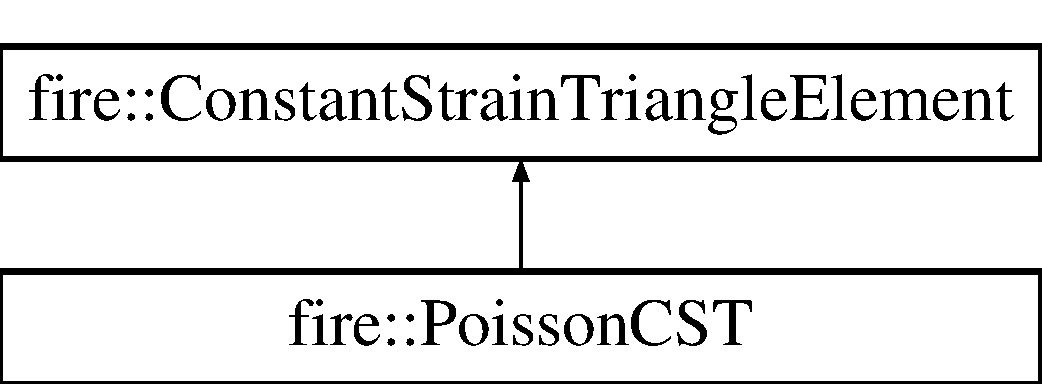
\includegraphics[height=5.000000cm]{a00770}
\end{center}
\end{figure}
\subsection*{Public Member Functions}
\begin{DoxyCompactItemize}
\item 
virtual void \hyperlink{a00770_a0dbeff2b9bd8dbfb2aad7a424eef87d1}{set\+Source} (const std\+::string \&source)=0
\item 
virtual const std\+::string \& \hyperlink{a00770_ab55d2644dfa6d950d1f874e1e02df095}{get\+Source} ()=0
\item 
virtual void \hyperlink{a00770_a7748a633910e9bfc27411d6bd840496b}{set\+Source} (const std\+::istream \&source)=0
\item 
virtual const std\+::istream \& \hyperlink{a00770_ac94c7a288bf669322b93ba171c43f90e}{get\+Source\+Stream} ()=0
\item 
virtual void \hyperlink{a00770_af36ac6eedd8c27d2f418869193d7d03c}{parse} ()=0
\item 
virtual bool \hyperlink{a00770_a616c42c85d781c916e97f0ad8f1e9010}{is\+File} ()=0
\item 
virtual bool \hyperlink{a00770_a97b9e58493b3cadbc63e670b0b0e759f}{is\+Local} ()=0
\item 
virtual bool \hyperlink{a00770_a83d2882a466d694fb0aea3d846bcbed4}{is\+Parallel} ()=0
\end{DoxyCompactItemize}


\subsection{Detailed Description}
This is the base interface for parsers in Fire and it defines the contract that can be expected of all parsers.

This source string is only a reference to the source or some sort of handle that points to it, such as a file or stream name. The exact type of the source -\/ file, stream, socket, etc. -\/ is determined by the implementing class. Check the documentation of implementing classes for the exact way the source string is used.

I\+Parsers should always be used by setting the source and then parsing the source\+:


\begin{DoxyCode}
IParser parser = ...;\textcolor{comment}{// somehow create your parser}
parser.setSource(sourceName);
parser.parser();
\end{DoxyCode}


Subclasses must always be sure that they implement \hyperlink{a00770_af36ac6eedd8c27d2f418869193d7d03c}{parse()} and \hyperlink{a00770_a0dbeff2b9bd8dbfb2aad7a424eef87d1}{set\+Source()}. 

\subsection{Member Function Documentation}
\mbox{\Hypertarget{a00770_ab55d2644dfa6d950d1f874e1e02df095}\label{a00770_ab55d2644dfa6d950d1f874e1e02df095}} 
\index{fire\+::\+I\+Parser@{fire\+::\+I\+Parser}!get\+Source@{get\+Source}}
\index{get\+Source@{get\+Source}!fire\+::\+I\+Parser@{fire\+::\+I\+Parser}}
\subsubsection{\texorpdfstring{get\+Source()}{getSource()}}
{\footnotesize\ttfamily virtual const std\+::string\& fire\+::\+I\+Parser\+::get\+Source (\begin{DoxyParamCaption}{ }\end{DoxyParamCaption})\hspace{0.3cm}{\ttfamily [pure virtual]}}

This operation gets the data source for the parser. \begin{DoxyReturn}{Returns}
the name of the source 
\end{DoxyReturn}


Implemented in \hyperlink{a00778_aedb7fe10911182525a719963b9b56726}{fire\+::\+Local\+Parser$<$ T $>$}, \hyperlink{a00778_aedb7fe10911182525a719963b9b56726}{fire\+::\+Local\+Parser$<$ std\+::string $>$}, and \hyperlink{a00766_ad02c9a530f20a706d7bb2554813e8d3a}{fire\+::\+I\+N\+I\+Property\+Parser}.

\mbox{\Hypertarget{a00770_ac94c7a288bf669322b93ba171c43f90e}\label{a00770_ac94c7a288bf669322b93ba171c43f90e}} 
\index{fire\+::\+I\+Parser@{fire\+::\+I\+Parser}!get\+Source\+Stream@{get\+Source\+Stream}}
\index{get\+Source\+Stream@{get\+Source\+Stream}!fire\+::\+I\+Parser@{fire\+::\+I\+Parser}}
\subsubsection{\texorpdfstring{get\+Source\+Stream()}{getSourceStream()}}
{\footnotesize\ttfamily virtual const std\+::istream\& fire\+::\+I\+Parser\+::get\+Source\+Stream (\begin{DoxyParamCaption}{ }\end{DoxyParamCaption})\hspace{0.3cm}{\ttfamily [pure virtual]}}

This operation gets the data source for the parser as a stream if and only if it was set as such. \begin{DoxyReturn}{Returns}
source the stream of delimited text data 
\end{DoxyReturn}


Implemented in \hyperlink{a00778_a9bf19a3cc9ae8ac0e6e7a0e7f6212cdc}{fire\+::\+Local\+Parser$<$ T $>$}, and \hyperlink{a00778_a9bf19a3cc9ae8ac0e6e7a0e7f6212cdc}{fire\+::\+Local\+Parser$<$ std\+::string $>$}.

\mbox{\Hypertarget{a00770_a616c42c85d781c916e97f0ad8f1e9010}\label{a00770_a616c42c85d781c916e97f0ad8f1e9010}} 
\index{fire\+::\+I\+Parser@{fire\+::\+I\+Parser}!is\+File@{is\+File}}
\index{is\+File@{is\+File}!fire\+::\+I\+Parser@{fire\+::\+I\+Parser}}
\subsubsection{\texorpdfstring{is\+File()}{isFile()}}
{\footnotesize\ttfamily virtual bool fire\+::\+I\+Parser\+::is\+File (\begin{DoxyParamCaption}{ }\end{DoxyParamCaption})\hspace{0.3cm}{\ttfamily [pure virtual]}}

This operation indicates whether or not the parser\textquotesingle{}s source is a file. \begin{DoxyReturn}{Returns}
true if this parser is working with a file, false otherwise. 
\end{DoxyReturn}


Implemented in \hyperlink{a00762_a091d5cf56bf8f407854ef87f460b2958}{fire\+::\+I\+Local\+Parser$<$ T $>$}, and \hyperlink{a00762_a091d5cf56bf8f407854ef87f460b2958}{fire\+::\+I\+Local\+Parser$<$ std\+::string $>$}.

\mbox{\Hypertarget{a00770_a97b9e58493b3cadbc63e670b0b0e759f}\label{a00770_a97b9e58493b3cadbc63e670b0b0e759f}} 
\index{fire\+::\+I\+Parser@{fire\+::\+I\+Parser}!is\+Local@{is\+Local}}
\index{is\+Local@{is\+Local}!fire\+::\+I\+Parser@{fire\+::\+I\+Parser}}
\subsubsection{\texorpdfstring{is\+Local()}{isLocal()}}
{\footnotesize\ttfamily virtual bool fire\+::\+I\+Parser\+::is\+Local (\begin{DoxyParamCaption}{ }\end{DoxyParamCaption})\hspace{0.3cm}{\ttfamily [pure virtual]}}

This operation indicates whether or not the parser is using a local source. \begin{DoxyReturn}{Returns}
true if this parser is working with a local source, false otherwise. 
\end{DoxyReturn}


Implemented in \hyperlink{a00762_a770acae6e216de3a9c7140a12de25d58}{fire\+::\+I\+Local\+Parser$<$ T $>$}, and \hyperlink{a00762_a770acae6e216de3a9c7140a12de25d58}{fire\+::\+I\+Local\+Parser$<$ std\+::string $>$}.

\mbox{\Hypertarget{a00770_a83d2882a466d694fb0aea3d846bcbed4}\label{a00770_a83d2882a466d694fb0aea3d846bcbed4}} 
\index{fire\+::\+I\+Parser@{fire\+::\+I\+Parser}!is\+Parallel@{is\+Parallel}}
\index{is\+Parallel@{is\+Parallel}!fire\+::\+I\+Parser@{fire\+::\+I\+Parser}}
\subsubsection{\texorpdfstring{is\+Parallel()}{isParallel()}}
{\footnotesize\ttfamily virtual bool fire\+::\+I\+Parser\+::is\+Parallel (\begin{DoxyParamCaption}{ }\end{DoxyParamCaption})\hspace{0.3cm}{\ttfamily [pure virtual]}}

This operation indicates whether or not the parser reads in parallel. \begin{DoxyReturn}{Returns}
true if this parser reads in parallel, false otherwise. 
\end{DoxyReturn}


Implemented in \hyperlink{a00762_ad46898c516adcce38acbb4800dc9777b}{fire\+::\+I\+Local\+Parser$<$ T $>$}, and \hyperlink{a00762_ad46898c516adcce38acbb4800dc9777b}{fire\+::\+I\+Local\+Parser$<$ std\+::string $>$}.

\mbox{\Hypertarget{a00770_af36ac6eedd8c27d2f418869193d7d03c}\label{a00770_af36ac6eedd8c27d2f418869193d7d03c}} 
\index{fire\+::\+I\+Parser@{fire\+::\+I\+Parser}!parse@{parse}}
\index{parse@{parse}!fire\+::\+I\+Parser@{fire\+::\+I\+Parser}}
\subsubsection{\texorpdfstring{parse()}{parse()}}
{\footnotesize\ttfamily virtual void fire\+::\+I\+Parser\+::parse (\begin{DoxyParamCaption}{ }\end{DoxyParamCaption})\hspace{0.3cm}{\ttfamily [pure virtual]}}

This operation directs the parser to parse its source. 

Implemented in \hyperlink{a00758_a773fa7ed28cb9d8c384ad94bd81fc93f}{fire\+::\+Delimited\+Text\+Parser$<$ T, K $>$}, \hyperlink{a00758_a686df5548771cae833d5e721442a821a}{fire\+::\+Delimited\+Text\+Parser$<$ T, K $>$}, \hyperlink{a00778_abd8929aea06c2dda40256d2e58236650}{fire\+::\+Local\+Parser$<$ T $>$}, \hyperlink{a00778_abd8929aea06c2dda40256d2e58236650}{fire\+::\+Local\+Parser$<$ std\+::string $>$}, \hyperlink{a00766_a31b6bad01e65ed4bb5f1ba297616c641}{fire\+::\+I\+N\+I\+Property\+Parser}, \hyperlink{a00778_ae904e264fe16708b3e434adea59e1b88}{fire\+::\+Local\+Parser$<$ T $>$}, \hyperlink{a00778_ae904e264fe16708b3e434adea59e1b88}{fire\+::\+Local\+Parser$<$ std\+::string $>$}, \hyperlink{a00778_a34fd9ffb0196c612c75b5288ed5e219b}{fire\+::\+Local\+Parser$<$ T $>$}, and \hyperlink{a00778_a34fd9ffb0196c612c75b5288ed5e219b}{fire\+::\+Local\+Parser$<$ std\+::string $>$}.

\mbox{\Hypertarget{a00770_a0dbeff2b9bd8dbfb2aad7a424eef87d1}\label{a00770_a0dbeff2b9bd8dbfb2aad7a424eef87d1}} 
\index{fire\+::\+I\+Parser@{fire\+::\+I\+Parser}!set\+Source@{set\+Source}}
\index{set\+Source@{set\+Source}!fire\+::\+I\+Parser@{fire\+::\+I\+Parser}}
\subsubsection{\texorpdfstring{set\+Source()}{setSource()}\hspace{0.1cm}{\footnotesize\ttfamily [1/2]}}
{\footnotesize\ttfamily virtual void fire\+::\+I\+Parser\+::set\+Source (\begin{DoxyParamCaption}\item[{const std\+::string \&}]{source }\end{DoxyParamCaption})\hspace{0.3cm}{\ttfamily [pure virtual]}}

This operation sets the data source for the parser. 
\begin{DoxyParams}{Parameters}
{\em source} & the name of the source that the parser should parse. \\
\hline
\end{DoxyParams}


Implemented in \hyperlink{a00778_afcaec6429fdd6e5d53642a32c001ff73}{fire\+::\+Local\+Parser$<$ T $>$}, \hyperlink{a00778_afcaec6429fdd6e5d53642a32c001ff73}{fire\+::\+Local\+Parser$<$ std\+::string $>$}, and \hyperlink{a00766_a06793909bc707a69d0c5772b14bc946d}{fire\+::\+I\+N\+I\+Property\+Parser}.

\mbox{\Hypertarget{a00770_a7748a633910e9bfc27411d6bd840496b}\label{a00770_a7748a633910e9bfc27411d6bd840496b}} 
\index{fire\+::\+I\+Parser@{fire\+::\+I\+Parser}!set\+Source@{set\+Source}}
\index{set\+Source@{set\+Source}!fire\+::\+I\+Parser@{fire\+::\+I\+Parser}}
\subsubsection{\texorpdfstring{set\+Source()}{setSource()}\hspace{0.1cm}{\footnotesize\ttfamily [2/2]}}
{\footnotesize\ttfamily virtual void fire\+::\+I\+Parser\+::set\+Source (\begin{DoxyParamCaption}\item[{const std\+::istream \&}]{source }\end{DoxyParamCaption})\hspace{0.3cm}{\ttfamily [pure virtual]}}

This operation sets the data source for the parser using a stream instead of a string. 
\begin{DoxyParams}{Parameters}
{\em source} & the stream of delimited text data \\
\hline
\end{DoxyParams}


Implemented in \hyperlink{a00778_aed4357541f2ff7d46f8846bd07bb3c42}{fire\+::\+Local\+Parser$<$ T $>$}, and \hyperlink{a00778_aed4357541f2ff7d46f8846bd07bb3c42}{fire\+::\+Local\+Parser$<$ std\+::string $>$}.



The documentation for this class was generated from the following file\+:\begin{DoxyCompactItemize}
\item 
I\+Parser.\+h\end{DoxyCompactItemize}

\hypertarget{a00774}{}\section{fire\+:\+:I\+Property\+Parser Class Reference}
\label{a00774}\index{fire\+::\+I\+Property\+Parser@{fire\+::\+I\+Property\+Parser}}


{\ttfamily \#include $<$I\+Property\+Parser.\+h$>$}

Inheritance diagram for fire\+:\+:I\+Property\+Parser\+:\begin{figure}[H]
\begin{center}
\leavevmode
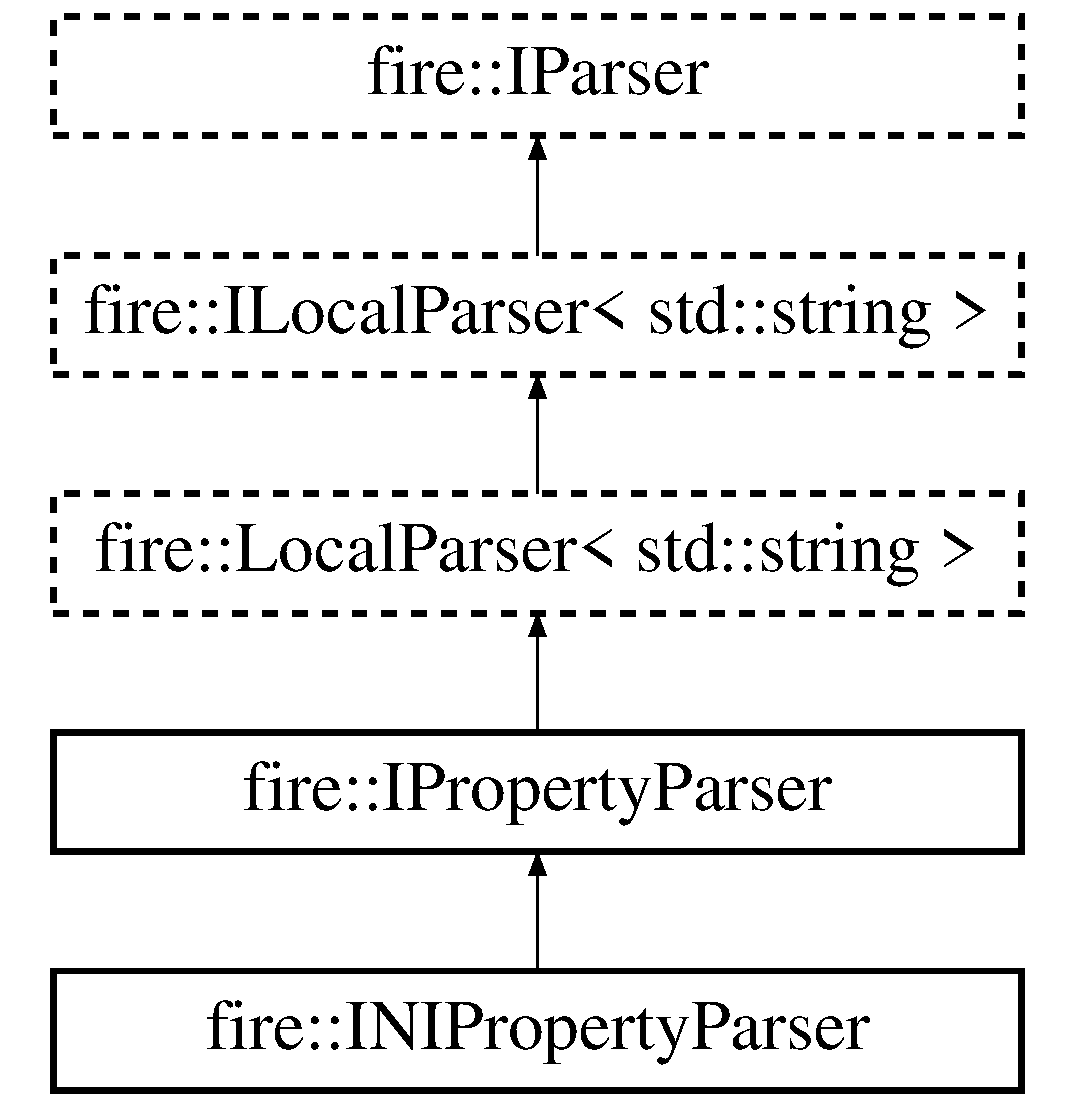
\includegraphics[height=5.000000cm]{a00774}
\end{center}
\end{figure}
\subsection*{Public Member Functions}
\begin{DoxyCompactItemize}
\item 
virtual const std\+::vector$<$ std\+::string $>$ \& \hyperlink{a00774_a34602687f9d1affac7bd842102d4a6aa}{get\+Property\+Block\+Names} ()=0
\item 
virtual const std\+::map$<$ std\+::string, std\+::string $>$ \& \hyperlink{a00774_a34201371cb36dd09e96a66242ececb86}{get\+Property\+Block} (const std\+::string \&name)=0
\end{DoxyCompactItemize}
\subsection*{Additional Inherited Members}


\subsection{Detailed Description}
This is an extension of the parser interface that focuses on parsing a set of properties. Properties are returned in blocks represented by maps.. 

\subsection{Member Function Documentation}
\mbox{\Hypertarget{a00774_a34201371cb36dd09e96a66242ececb86}\label{a00774_a34201371cb36dd09e96a66242ececb86}} 
\index{fire\+::\+I\+Property\+Parser@{fire\+::\+I\+Property\+Parser}!get\+Property\+Block@{get\+Property\+Block}}
\index{get\+Property\+Block@{get\+Property\+Block}!fire\+::\+I\+Property\+Parser@{fire\+::\+I\+Property\+Parser}}
\subsubsection{\texorpdfstring{get\+Property\+Block()}{getPropertyBlock()}}
{\footnotesize\ttfamily virtual const std\+::map$<$std\+::string, std\+::string$>$\& fire\+::\+I\+Property\+Parser\+::get\+Property\+Block (\begin{DoxyParamCaption}\item[{const std\+::string \&}]{name }\end{DoxyParamCaption})\hspace{0.3cm}{\ttfamily [pure virtual]}}

This operation returns the property block with the given name. 
\begin{DoxyParams}{Parameters}
{\em name} & the block name \\
\hline
\end{DoxyParams}
\begin{DoxyReturn}{Returns}
the property block with the given name 
\end{DoxyReturn}


Implemented in \hyperlink{a00766_a3591312590a66659ebd377cdde9ab9ad}{fire\+::\+I\+N\+I\+Property\+Parser}.

\mbox{\Hypertarget{a00774_a34602687f9d1affac7bd842102d4a6aa}\label{a00774_a34602687f9d1affac7bd842102d4a6aa}} 
\index{fire\+::\+I\+Property\+Parser@{fire\+::\+I\+Property\+Parser}!get\+Property\+Block\+Names@{get\+Property\+Block\+Names}}
\index{get\+Property\+Block\+Names@{get\+Property\+Block\+Names}!fire\+::\+I\+Property\+Parser@{fire\+::\+I\+Property\+Parser}}
\subsubsection{\texorpdfstring{get\+Property\+Block\+Names()}{getPropertyBlockNames()}}
{\footnotesize\ttfamily virtual const std\+::vector$<$std\+::string$>$\& fire\+::\+I\+Property\+Parser\+::get\+Property\+Block\+Names (\begin{DoxyParamCaption}{ }\end{DoxyParamCaption})\hspace{0.3cm}{\ttfamily [pure virtual]}}

This operation returns the names of the property blocks parsed from the source. \begin{DoxyReturn}{Returns}
the block names 
\end{DoxyReturn}


Implemented in \hyperlink{a00766_aed0f1f47111794659564dcddb4d25bc6}{fire\+::\+I\+N\+I\+Property\+Parser}.



The documentation for this class was generated from the following file\+:\begin{DoxyCompactItemize}
\item 
I\+Property\+Parser.\+h\end{DoxyCompactItemize}

\hypertarget{a00746}{}\section{fire\+:\+:I\+Stepper Class Reference}
\label{a00746}\index{fire\+::\+I\+Stepper@{fire\+::\+I\+Stepper}}


{\ttfamily \#include $<$I\+Stepper.\+h$>$}

Inheritance diagram for fire\+:\+:I\+Stepper\+:\begin{figure}[H]
\begin{center}
\leavevmode
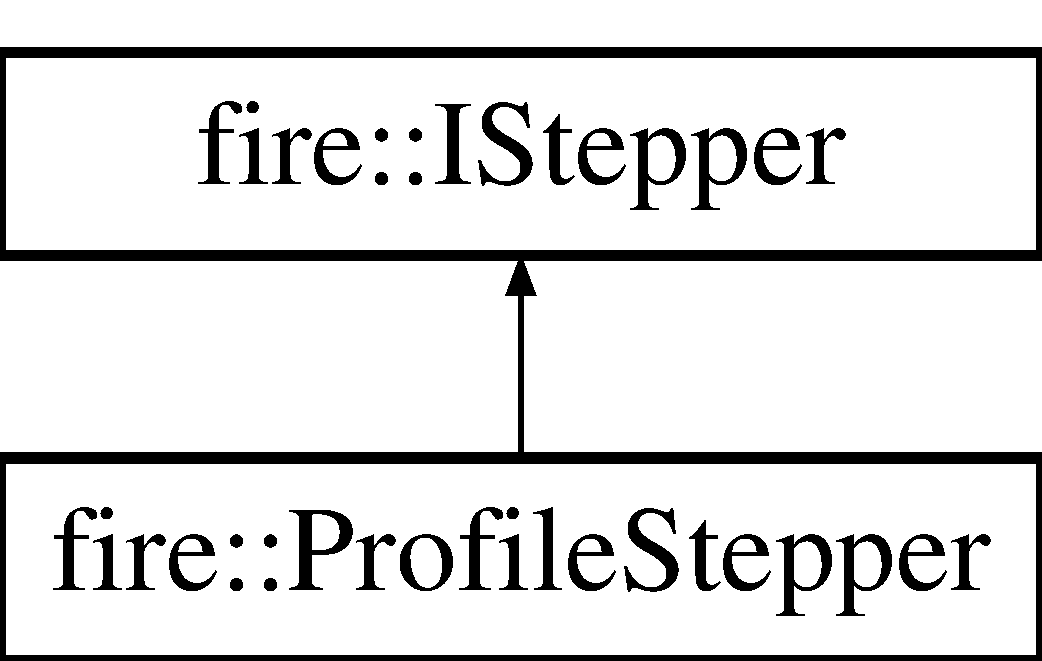
\includegraphics[height=2.000000cm]{a00746}
\end{center}
\end{figure}
\subsection*{Public Member Functions}
\begin{DoxyCompactItemize}
\item 
virtual double \hyperlink{a00746_a7f709d1462a2a3b8bd8214cc681ca26e}{get\+Step} ()=0
\item 
virtual double \hyperlink{a00746_a43027c0c268afcd59db8815c2e2c41ea}{get\+Step\+Size\+At\+Stage} (int i)=0
\item 
virtual void \hyperlink{a00746_a44dfccb90ee5ef6e080b54113c215458}{update\+Step} ()=0
\item 
virtual void \hyperlink{a00746_a3a5099cd0f3c874e56c33cb8f13b8f3b}{set\+Initial\+Step} (double initial\+Step)=0
\item 
virtual double \hyperlink{a00746_a49df3a2ac05cebaf2baf387b66d19272}{get\+Initial\+Step} ()=0
\item 
virtual void \hyperlink{a00746_add76974a7b6fbbc93916270a376c461e}{set\+Final\+Step} (double final\+Step)=0
\item 
virtual double \hyperlink{a00746_ab234d9f032e02668aededf1c22e8c0a9}{get\+Final\+Step} ()=0
\item 
virtual void \hyperlink{a00746_a69c262f248511efcd271be1724a41ad9}{set\+Initial\+Stepsize} (double step\+Size)=0
\item 
virtual double \hyperlink{a00746_afb777e62386b25e5a38d59af54972690}{get\+Initial\+Stepsize} ()=0
\item 
virtual \hyperlink{a00746_ac8ec460d35512e2e039396d5192eb57e}{$\sim$\+I\+Stepper} ()
\end{DoxyCompactItemize}


\subsection{Detailed Description}
This is an interface for managing discrete steps as required by Initial Value Problem Integrators. \hyperlink{a00746}{I\+Stepper} implementations track both the step and the stepsize. In the case of time-\/dependent initial value problems, implementations would be called \char`\"{}time steppers\char`\"{} and would be responsible for computing both the present time (the step) and the step between the present size and the next (the step size). In purely spatial or otherwise on-\/temporal problems, the step represents the current value of the independent variable and the step size represents the distance between the present and next steps.

This interface is designed for single-\/ and multi-\/stage solvers, such as Runge-\/\+Kutta solvers. 

\subsection{Constructor \& Destructor Documentation}
\mbox{\Hypertarget{a00746_ac8ec460d35512e2e039396d5192eb57e}\label{a00746_ac8ec460d35512e2e039396d5192eb57e}} 
\index{fire\+::\+I\+Stepper@{fire\+::\+I\+Stepper}!````~I\+Stepper@{$\sim$\+I\+Stepper}}
\index{````~I\+Stepper@{$\sim$\+I\+Stepper}!fire\+::\+I\+Stepper@{fire\+::\+I\+Stepper}}
\subsubsection{\texorpdfstring{$\sim$\+I\+Stepper()}{~IStepper()}}
{\footnotesize\ttfamily virtual fire\+::\+I\+Stepper\+::$\sim$\+I\+Stepper (\begin{DoxyParamCaption}{ }\end{DoxyParamCaption})\hspace{0.3cm}{\ttfamily [inline]}, {\ttfamily [virtual]}}

Virtual Destructor 

\subsection{Member Function Documentation}
\mbox{\Hypertarget{a00746_ab234d9f032e02668aededf1c22e8c0a9}\label{a00746_ab234d9f032e02668aededf1c22e8c0a9}} 
\index{fire\+::\+I\+Stepper@{fire\+::\+I\+Stepper}!get\+Final\+Step@{get\+Final\+Step}}
\index{get\+Final\+Step@{get\+Final\+Step}!fire\+::\+I\+Stepper@{fire\+::\+I\+Stepper}}
\subsubsection{\texorpdfstring{get\+Final\+Step()}{getFinalStep()}}
{\footnotesize\ttfamily virtual double fire\+::\+I\+Stepper\+::get\+Final\+Step (\begin{DoxyParamCaption}{ }\end{DoxyParamCaption})\hspace{0.3cm}{\ttfamily [pure virtual]}}

This operation returns the final step for the stepper. \begin{DoxyReturn}{Returns}
the final step 
\end{DoxyReturn}


Implemented in \hyperlink{a00750_ae6f257aca7b3bb62a851169a01bcaacf}{fire\+::\+Profile\+Stepper}.

\mbox{\Hypertarget{a00746_a49df3a2ac05cebaf2baf387b66d19272}\label{a00746_a49df3a2ac05cebaf2baf387b66d19272}} 
\index{fire\+::\+I\+Stepper@{fire\+::\+I\+Stepper}!get\+Initial\+Step@{get\+Initial\+Step}}
\index{get\+Initial\+Step@{get\+Initial\+Step}!fire\+::\+I\+Stepper@{fire\+::\+I\+Stepper}}
\subsubsection{\texorpdfstring{get\+Initial\+Step()}{getInitialStep()}}
{\footnotesize\ttfamily virtual double fire\+::\+I\+Stepper\+::get\+Initial\+Step (\begin{DoxyParamCaption}{ }\end{DoxyParamCaption})\hspace{0.3cm}{\ttfamily [pure virtual]}}

This operation returns the initial step for the stepper. \begin{DoxyReturn}{Returns}
the initial step 
\end{DoxyReturn}


Implemented in \hyperlink{a00750_af24660fa4bd027f877d5c1bdeb286cf5}{fire\+::\+Profile\+Stepper}.

\mbox{\Hypertarget{a00746_afb777e62386b25e5a38d59af54972690}\label{a00746_afb777e62386b25e5a38d59af54972690}} 
\index{fire\+::\+I\+Stepper@{fire\+::\+I\+Stepper}!get\+Initial\+Stepsize@{get\+Initial\+Stepsize}}
\index{get\+Initial\+Stepsize@{get\+Initial\+Stepsize}!fire\+::\+I\+Stepper@{fire\+::\+I\+Stepper}}
\subsubsection{\texorpdfstring{get\+Initial\+Stepsize()}{getInitialStepsize()}}
{\footnotesize\ttfamily virtual double fire\+::\+I\+Stepper\+::get\+Initial\+Stepsize (\begin{DoxyParamCaption}{ }\end{DoxyParamCaption})\hspace{0.3cm}{\ttfamily [pure virtual]}}

This operation gets the initial step size for the stepper \begin{DoxyReturn}{Returns}
the initial step size 
\end{DoxyReturn}


Implemented in \hyperlink{a00750_a86e7035366907a08a36722655746271e}{fire\+::\+Profile\+Stepper}.

\mbox{\Hypertarget{a00746_a7f709d1462a2a3b8bd8214cc681ca26e}\label{a00746_a7f709d1462a2a3b8bd8214cc681ca26e}} 
\index{fire\+::\+I\+Stepper@{fire\+::\+I\+Stepper}!get\+Step@{get\+Step}}
\index{get\+Step@{get\+Step}!fire\+::\+I\+Stepper@{fire\+::\+I\+Stepper}}
\subsubsection{\texorpdfstring{get\+Step()}{getStep()}}
{\footnotesize\ttfamily virtual double fire\+::\+I\+Stepper\+::get\+Step (\begin{DoxyParamCaption}{ }\end{DoxyParamCaption})\hspace{0.3cm}{\ttfamily [pure virtual]}}

This operation returns the step value for the current step. \begin{DoxyReturn}{Returns}
the step value 
\end{DoxyReturn}


Implemented in \hyperlink{a00750_a9096ad65a3fcf63678b600cbe0c33961}{fire\+::\+Profile\+Stepper}.

\mbox{\Hypertarget{a00746_a43027c0c268afcd59db8815c2e2c41ea}\label{a00746_a43027c0c268afcd59db8815c2e2c41ea}} 
\index{fire\+::\+I\+Stepper@{fire\+::\+I\+Stepper}!get\+Step\+Size\+At\+Stage@{get\+Step\+Size\+At\+Stage}}
\index{get\+Step\+Size\+At\+Stage@{get\+Step\+Size\+At\+Stage}!fire\+::\+I\+Stepper@{fire\+::\+I\+Stepper}}
\subsubsection{\texorpdfstring{get\+Step\+Size\+At\+Stage()}{getStepSizeAtStage()}}
{\footnotesize\ttfamily virtual double fire\+::\+I\+Stepper\+::get\+Step\+Size\+At\+Stage (\begin{DoxyParamCaption}\item[{int}]{i }\end{DoxyParamCaption})\hspace{0.3cm}{\ttfamily [pure virtual]}}

This operation returns the step size for the given stage. 
\begin{DoxyParams}{Parameters}
{\em the} & stage of the solver for which the stepsize should be computed \\
\hline
\end{DoxyParams}
\begin{DoxyReturn}{Returns}
the step size 
\end{DoxyReturn}


Implemented in \hyperlink{a00750_adaa1a23c068977ecc6809dd8eecab49d}{fire\+::\+Profile\+Stepper}.

\mbox{\Hypertarget{a00746_add76974a7b6fbbc93916270a376c461e}\label{a00746_add76974a7b6fbbc93916270a376c461e}} 
\index{fire\+::\+I\+Stepper@{fire\+::\+I\+Stepper}!set\+Final\+Step@{set\+Final\+Step}}
\index{set\+Final\+Step@{set\+Final\+Step}!fire\+::\+I\+Stepper@{fire\+::\+I\+Stepper}}
\subsubsection{\texorpdfstring{set\+Final\+Step()}{setFinalStep()}}
{\footnotesize\ttfamily virtual void fire\+::\+I\+Stepper\+::set\+Final\+Step (\begin{DoxyParamCaption}\item[{double}]{final\+Step }\end{DoxyParamCaption})\hspace{0.3cm}{\ttfamily [pure virtual]}}

This operation sets the final step for the stepper. 
\begin{DoxyParams}{Parameters}
{\em final\+Step} & the final step \\
\hline
\end{DoxyParams}


Implemented in \hyperlink{a00750_af8203296b4f3bef53bafab7cb654cc97}{fire\+::\+Profile\+Stepper}.

\mbox{\Hypertarget{a00746_a3a5099cd0f3c874e56c33cb8f13b8f3b}\label{a00746_a3a5099cd0f3c874e56c33cb8f13b8f3b}} 
\index{fire\+::\+I\+Stepper@{fire\+::\+I\+Stepper}!set\+Initial\+Step@{set\+Initial\+Step}}
\index{set\+Initial\+Step@{set\+Initial\+Step}!fire\+::\+I\+Stepper@{fire\+::\+I\+Stepper}}
\subsubsection{\texorpdfstring{set\+Initial\+Step()}{setInitialStep()}}
{\footnotesize\ttfamily virtual void fire\+::\+I\+Stepper\+::set\+Initial\+Step (\begin{DoxyParamCaption}\item[{double}]{initial\+Step }\end{DoxyParamCaption})\hspace{0.3cm}{\ttfamily [pure virtual]}}

This operation sets the initial step for the stepper. 
\begin{DoxyParams}{Parameters}
{\em initial\+Step} & the initial step \\
\hline
\end{DoxyParams}


Implemented in \hyperlink{a00750_adf2f78648d9539282225117c0fd243af}{fire\+::\+Profile\+Stepper}.

\mbox{\Hypertarget{a00746_a69c262f248511efcd271be1724a41ad9}\label{a00746_a69c262f248511efcd271be1724a41ad9}} 
\index{fire\+::\+I\+Stepper@{fire\+::\+I\+Stepper}!set\+Initial\+Stepsize@{set\+Initial\+Stepsize}}
\index{set\+Initial\+Stepsize@{set\+Initial\+Stepsize}!fire\+::\+I\+Stepper@{fire\+::\+I\+Stepper}}
\subsubsection{\texorpdfstring{set\+Initial\+Stepsize()}{setInitialStepsize()}}
{\footnotesize\ttfamily virtual void fire\+::\+I\+Stepper\+::set\+Initial\+Stepsize (\begin{DoxyParamCaption}\item[{double}]{step\+Size }\end{DoxyParamCaption})\hspace{0.3cm}{\ttfamily [pure virtual]}}

This operation sets the initial step size for the stepper 
\begin{DoxyParams}{Parameters}
{\em the} & initial step size \\
\hline
\end{DoxyParams}


Implemented in \hyperlink{a00750_a55c44fd97d8b6a474243ad0da48b039d}{fire\+::\+Profile\+Stepper}.

\mbox{\Hypertarget{a00746_a44dfccb90ee5ef6e080b54113c215458}\label{a00746_a44dfccb90ee5ef6e080b54113c215458}} 
\index{fire\+::\+I\+Stepper@{fire\+::\+I\+Stepper}!update\+Step@{update\+Step}}
\index{update\+Step@{update\+Step}!fire\+::\+I\+Stepper@{fire\+::\+I\+Stepper}}
\subsubsection{\texorpdfstring{update\+Step()}{updateStep()}}
{\footnotesize\ttfamily virtual void fire\+::\+I\+Stepper\+::update\+Step (\begin{DoxyParamCaption}{ }\end{DoxyParamCaption})\hspace{0.3cm}{\ttfamily [pure virtual]}}

This operation replaces the current step and stepsize with the next step and stepsize values. 

Implemented in \hyperlink{a00750_a2c13fd4da5550f1e58df2b54bbfe4c2c}{fire\+::\+Profile\+Stepper}.



The documentation for this class was generated from the following file\+:\begin{DoxyCompactItemize}
\item 
I\+Stepper.\+h\end{DoxyCompactItemize}

\hypertarget{a00814}{}\section{fire\+:\+:I\+N\+I\+Property\+Parser Class Reference}
\label{a00814}\index{fire\+::\+I\+N\+I\+Property\+Parser@{fire\+::\+I\+N\+I\+Property\+Parser}}


{\ttfamily \#include $<$I\+N\+I\+Property\+Parser.\+h$>$}

Inheritance diagram for fire\+:\+:I\+N\+I\+Property\+Parser\+:\begin{figure}[H]
\begin{center}
\leavevmode
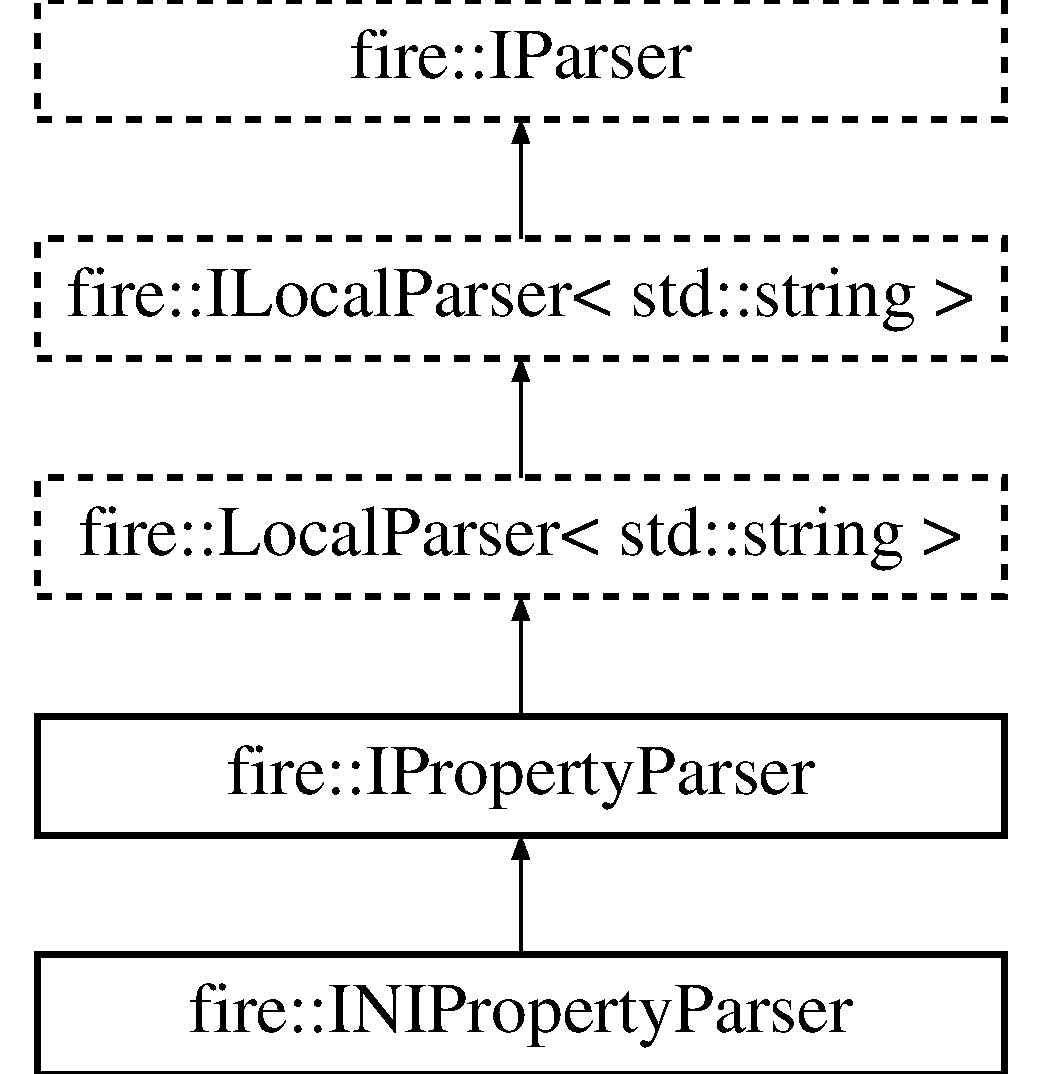
\includegraphics[height=5.000000cm]{a00814}
\end{center}
\end{figure}
\subsection*{Public Member Functions}
\begin{DoxyCompactItemize}
\item 
virtual void \hyperlink{a00814_a06793909bc707a69d0c5772b14bc946d}{set\+Source} (const std\+::string \&source)
\item 
virtual const std\+::string \& \hyperlink{a00814_ad02c9a530f20a706d7bb2554813e8d3a}{get\+Source} ()
\item 
virtual void \hyperlink{a00814_a31b6bad01e65ed4bb5f1ba297616c641}{parse} ()
\item 
virtual const std\+::vector$<$ std\+::string $>$ \& \hyperlink{a00814_aed0f1f47111794659564dcddb4d25bc6}{get\+Property\+Block\+Names} ()
\item 
virtual const std\+::map$<$ std\+::string, std\+::string $>$ \& \hyperlink{a00814_a3591312590a66659ebd377cdde9ab9ad}{get\+Property\+Block} (const std\+::string \&name)
\end{DoxyCompactItemize}
\subsection*{Additional Inherited Members}


\subsection{Detailed Description}
This class implements \hyperlink{a00822}{I\+Property\+Parser} to provide a local, file-\/based, serially executed I\+NI parser.

\hyperlink{a00810_a091d5cf56bf8f407854ef87f460b2958}{is\+File()} always returns true. \hyperlink{a00810_a770acae6e216de3a9c7140a12de25d58}{is\+Local()} always returns true. \hyperlink{a00810_ad46898c516adcce38acbb4800dc9777b}{is\+Parallel()} always returns false.

This implementation is backed by Simple\+I\+NI, one of Fire\textquotesingle{}s dependencies, so it supports whatever Simple\+I\+NI supports.

The source must be a file on the local filesystem. 

\subsection{Member Function Documentation}
\mbox{\Hypertarget{a00814_a3591312590a66659ebd377cdde9ab9ad}\label{a00814_a3591312590a66659ebd377cdde9ab9ad}} 
\index{fire\+::\+I\+N\+I\+Property\+Parser@{fire\+::\+I\+N\+I\+Property\+Parser}!get\+Property\+Block@{get\+Property\+Block}}
\index{get\+Property\+Block@{get\+Property\+Block}!fire\+::\+I\+N\+I\+Property\+Parser@{fire\+::\+I\+N\+I\+Property\+Parser}}
\subsubsection{\texorpdfstring{get\+Property\+Block()}{getPropertyBlock()}}
{\footnotesize\ttfamily virtual const std\+::map$<$std\+::string, std\+::string$>$\& fire\+::\+I\+N\+I\+Property\+Parser\+::get\+Property\+Block (\begin{DoxyParamCaption}\item[{const std\+::string \&}]{name }\end{DoxyParamCaption})\hspace{0.3cm}{\ttfamily [inline]}, {\ttfamily [virtual]}}

This operation returns the property block with the given name. 
\begin{DoxyParams}{Parameters}
{\em name} & the block name \\
\hline
\end{DoxyParams}
\begin{DoxyReturn}{Returns}
the property block with the given name 
\end{DoxyReturn}


Implements \hyperlink{a00822_a34201371cb36dd09e96a66242ececb86}{fire\+::\+I\+Property\+Parser}.

\mbox{\Hypertarget{a00814_aed0f1f47111794659564dcddb4d25bc6}\label{a00814_aed0f1f47111794659564dcddb4d25bc6}} 
\index{fire\+::\+I\+N\+I\+Property\+Parser@{fire\+::\+I\+N\+I\+Property\+Parser}!get\+Property\+Block\+Names@{get\+Property\+Block\+Names}}
\index{get\+Property\+Block\+Names@{get\+Property\+Block\+Names}!fire\+::\+I\+N\+I\+Property\+Parser@{fire\+::\+I\+N\+I\+Property\+Parser}}
\subsubsection{\texorpdfstring{get\+Property\+Block\+Names()}{getPropertyBlockNames()}}
{\footnotesize\ttfamily virtual const std\+::vector$<$std\+::string$>$\& fire\+::\+I\+N\+I\+Property\+Parser\+::get\+Property\+Block\+Names (\begin{DoxyParamCaption}{ }\end{DoxyParamCaption})\hspace{0.3cm}{\ttfamily [inline]}, {\ttfamily [virtual]}}

This operation returns the names of the property blocks parsed from the source. \begin{DoxyReturn}{Returns}
the block names 
\end{DoxyReturn}


Implements \hyperlink{a00822_a34602687f9d1affac7bd842102d4a6aa}{fire\+::\+I\+Property\+Parser}.

\mbox{\Hypertarget{a00814_ad02c9a530f20a706d7bb2554813e8d3a}\label{a00814_ad02c9a530f20a706d7bb2554813e8d3a}} 
\index{fire\+::\+I\+N\+I\+Property\+Parser@{fire\+::\+I\+N\+I\+Property\+Parser}!get\+Source@{get\+Source}}
\index{get\+Source@{get\+Source}!fire\+::\+I\+N\+I\+Property\+Parser@{fire\+::\+I\+N\+I\+Property\+Parser}}
\subsubsection{\texorpdfstring{get\+Source()}{getSource()}}
{\footnotesize\ttfamily virtual const std\+::string\& fire\+::\+I\+N\+I\+Property\+Parser\+::get\+Source (\begin{DoxyParamCaption}{ }\end{DoxyParamCaption})\hspace{0.3cm}{\ttfamily [inline]}, {\ttfamily [virtual]}}

This operation gets the data source for the parser. \begin{DoxyReturn}{Returns}
the name of the source 
\end{DoxyReturn}


Reimplemented from \hyperlink{a00826_aedb7fe10911182525a719963b9b56726}{fire\+::\+Local\+Parser$<$ std\+::string $>$}.

\mbox{\Hypertarget{a00814_a31b6bad01e65ed4bb5f1ba297616c641}\label{a00814_a31b6bad01e65ed4bb5f1ba297616c641}} 
\index{fire\+::\+I\+N\+I\+Property\+Parser@{fire\+::\+I\+N\+I\+Property\+Parser}!parse@{parse}}
\index{parse@{parse}!fire\+::\+I\+N\+I\+Property\+Parser@{fire\+::\+I\+N\+I\+Property\+Parser}}
\subsubsection{\texorpdfstring{parse()}{parse()}}
{\footnotesize\ttfamily virtual void fire\+::\+I\+N\+I\+Property\+Parser\+::parse (\begin{DoxyParamCaption}{ }\end{DoxyParamCaption})\hspace{0.3cm}{\ttfamily [inline]}, {\ttfamily [virtual]}}

This operation directs the parser to parse its source. 

Reimplemented from \hyperlink{a00826_abd8929aea06c2dda40256d2e58236650}{fire\+::\+Local\+Parser$<$ std\+::string $>$}.

\mbox{\Hypertarget{a00814_a06793909bc707a69d0c5772b14bc946d}\label{a00814_a06793909bc707a69d0c5772b14bc946d}} 
\index{fire\+::\+I\+N\+I\+Property\+Parser@{fire\+::\+I\+N\+I\+Property\+Parser}!set\+Source@{set\+Source}}
\index{set\+Source@{set\+Source}!fire\+::\+I\+N\+I\+Property\+Parser@{fire\+::\+I\+N\+I\+Property\+Parser}}
\subsubsection{\texorpdfstring{set\+Source()}{setSource()}}
{\footnotesize\ttfamily virtual void fire\+::\+I\+N\+I\+Property\+Parser\+::set\+Source (\begin{DoxyParamCaption}\item[{const std\+::string \&}]{source }\end{DoxyParamCaption})\hspace{0.3cm}{\ttfamily [inline]}, {\ttfamily [virtual]}}

This operation sets the data source for the parser. 
\begin{DoxyParams}{Parameters}
{\em source} & the name of the source that the parser should parse. \\
\hline
\end{DoxyParams}


Reimplemented from \hyperlink{a00826_afcaec6429fdd6e5d53642a32c001ff73}{fire\+::\+Local\+Parser$<$ std\+::string $>$}.



The documentation for this class was generated from the following file\+:\begin{DoxyCompactItemize}
\item 
I\+N\+I\+Property\+Parser.\+h\end{DoxyCompactItemize}

\hypertarget{a00882}{}\section{C\+Simple\+Ini\+Templ$<$ S\+I\+\_\+\+C\+H\+AR, S\+I\+\_\+\+S\+T\+R\+L\+E\+SS, S\+I\+\_\+\+C\+O\+N\+V\+E\+R\+T\+ER $>$ Class Template Reference}
\label{a00882}\index{C\+Simple\+Ini\+Templ$<$ S\+I\+\_\+\+C\+H\+A\+R, S\+I\+\_\+\+S\+T\+R\+L\+E\+S\+S, S\+I\+\_\+\+C\+O\+N\+V\+E\+R\+T\+E\+R $>$@{C\+Simple\+Ini\+Templ$<$ S\+I\+\_\+\+C\+H\+A\+R, S\+I\+\_\+\+S\+T\+R\+L\+E\+S\+S, S\+I\+\_\+\+C\+O\+N\+V\+E\+R\+T\+E\+R $>$}}


{\ttfamily \#include $<$Simple\+Ini.\+h$>$}

\subsection*{Classes}
\begin{DoxyCompactItemize}
\item 
class \hyperlink{a00910}{Converter}
\item 
struct \hyperlink{a00886}{Entry}
\item 
class \hyperlink{a00902}{File\+Writer}
\item 
class \hyperlink{a00898}{Output\+Writer}
\item 
class \hyperlink{a00906}{String\+Writer}
\end{DoxyCompactItemize}
\subsection*{Public Types}
\begin{DoxyCompactItemize}
\item 
\mbox{\Hypertarget{a00882_ad7ffad7e87da2303a05b885e95bc74fa}\label{a00882_ad7ffad7e87da2303a05b885e95bc74fa}} 
typedef S\+I\+\_\+\+C\+H\+AR {\bfseries S\+I\+\_\+\+C\+H\+A\+R\+\_\+T}
\item 
typedef std\+::multimap$<$ \hyperlink{a00886}{Entry}, const S\+I\+\_\+\+C\+H\+AR $\ast$, typename \hyperlink{a00890}{Entry\+::\+Key\+Order} $>$ \hyperlink{a00882_ae7f0e11d84617214bd479de6332c80e6}{T\+Key\+Val}
\item 
typedef std\+::map$<$ \hyperlink{a00886}{Entry}, \hyperlink{a00882_ae7f0e11d84617214bd479de6332c80e6}{T\+Key\+Val}, typename \hyperlink{a00890}{Entry\+::\+Key\+Order} $>$ \hyperlink{a00882_a2e7963455f680abd0d6901786495a665}{T\+Section}
\item 
typedef std\+::list$<$ \hyperlink{a00886}{Entry} $>$ \hyperlink{a00882_a391b3f3751e06cd9e9de4fb16ac14342}{T\+Names\+Depend}
\end{DoxyCompactItemize}
\subsection*{Public Member Functions}
\begin{DoxyCompactItemize}
\item 
\hyperlink{a00882_af878d0a2aa780255b621e95f58f691d8}{C\+Simple\+Ini\+Templ} (bool a\+\_\+b\+Is\+Utf8=false, bool a\+\_\+b\+Multi\+Key=false, bool a\+\_\+b\+Multi\+Line=false)
\item 
\hyperlink{a00882_a8c933adc1d46bb663caeb6f9dee5aa12}{$\sim$\+C\+Simple\+Ini\+Templ} ()
\item 
void \hyperlink{a00882_a89b34d38be4518e9ed91c634a41b8055}{Reset} ()
\item 
bool \hyperlink{a00882_a54bbe9727db17b368a0a75abd5e52d1c}{Is\+Empty} () const
\item 
S\+I\+\_\+\+Error \hyperlink{a00882_aebb6e5fff76efc05ca6cc4b7b56481a3}{Load\+File} (const char $\ast$a\+\_\+psz\+File)
\item 
S\+I\+\_\+\+Error \hyperlink{a00882_a7ccb65e82fa347b42b59330968f826ae}{Load\+File} (F\+I\+LE $\ast$a\+\_\+fp\+File)
\item 
S\+I\+\_\+\+Error \hyperlink{a00882_a174244fd3e09ff78da05fe46be86e714}{Load\+Data} (const std\+::string \&a\+\_\+str\+Data)
\item 
S\+I\+\_\+\+Error \hyperlink{a00882_aa797cf47cec05906f07d5065882af4d3}{Load\+Data} (const char $\ast$a\+\_\+p\+Data, size\+\_\+t a\+\_\+u\+Data\+Len)
\item 
S\+I\+\_\+\+Error \hyperlink{a00882_af00e754689a94cbe87b387f99f7a5d01}{Save\+File} (const char $\ast$a\+\_\+psz\+File, bool a\+\_\+b\+Add\+Signature=true) const
\item 
S\+I\+\_\+\+Error \hyperlink{a00882_a3c3f677c1515e08751cb52a1dfaf1a93}{Save\+File} (F\+I\+LE $\ast$a\+\_\+p\+File, bool a\+\_\+b\+Add\+Signature=false) const
\item 
S\+I\+\_\+\+Error \hyperlink{a00882_a6ec10daab297e92cdffe024ba5e6d999}{Save} (\hyperlink{a00898}{Output\+Writer} \&a\+\_\+o\+Output, bool a\+\_\+b\+Add\+Signature=false) const
\item 
S\+I\+\_\+\+Error \hyperlink{a00882_a9fc5894f12a31b8496a9627cd0f42139}{Save} (std\+::string \&a\+\_\+s\+Buffer, bool a\+\_\+b\+Add\+Signature=false) const
\item 
void \hyperlink{a00882_a7fe8a8b70b0ef000c591011a8332ebd5}{Get\+All\+Sections} (\hyperlink{a00882_a391b3f3751e06cd9e9de4fb16ac14342}{T\+Names\+Depend} \&a\+\_\+names) const
\item 
bool \hyperlink{a00882_a08cadb6624a6c459703efaadb25d31c9}{Get\+All\+Keys} (const S\+I\+\_\+\+C\+H\+AR $\ast$a\+\_\+p\+Section, \hyperlink{a00882_a391b3f3751e06cd9e9de4fb16ac14342}{T\+Names\+Depend} \&a\+\_\+names) const
\item 
bool \hyperlink{a00882_adda5ee7f422695f7e67be2d066e303bf}{Get\+All\+Values} (const S\+I\+\_\+\+C\+H\+AR $\ast$a\+\_\+p\+Section, const S\+I\+\_\+\+C\+H\+AR $\ast$a\+\_\+p\+Key, \hyperlink{a00882_a391b3f3751e06cd9e9de4fb16ac14342}{T\+Names\+Depend} \&a\+\_\+values) const
\item 
int \hyperlink{a00882_a0a9c089eabb5faf764c4af449f7b1846}{Get\+Section\+Size} (const S\+I\+\_\+\+C\+H\+AR $\ast$a\+\_\+p\+Section) const
\item 
const \hyperlink{a00882_ae7f0e11d84617214bd479de6332c80e6}{T\+Key\+Val} $\ast$ \hyperlink{a00882_a56a6838556328ab8bfaa7ded9edb9c8a}{Get\+Section} (const S\+I\+\_\+\+C\+H\+AR $\ast$a\+\_\+p\+Section) const
\item 
const S\+I\+\_\+\+C\+H\+AR $\ast$ \hyperlink{a00882_a74e3f5d22f50b70b2a20c89ec7e2c737}{Get\+Value} (const S\+I\+\_\+\+C\+H\+AR $\ast$a\+\_\+p\+Section, const S\+I\+\_\+\+C\+H\+AR $\ast$a\+\_\+p\+Key, const S\+I\+\_\+\+C\+H\+AR $\ast$a\+\_\+p\+Default=N\+U\+LL, bool $\ast$a\+\_\+p\+Has\+Multiple=N\+U\+LL) const
\item 
long \hyperlink{a00882_a7fa211c1c768497520eab7f2014ae786}{Get\+Long\+Value} (const S\+I\+\_\+\+C\+H\+AR $\ast$a\+\_\+p\+Section, const S\+I\+\_\+\+C\+H\+AR $\ast$a\+\_\+p\+Key, long a\+\_\+n\+Default=0, bool $\ast$a\+\_\+p\+Has\+Multiple=N\+U\+LL) const
\item 
double \hyperlink{a00882_aab58a949481926cf1d42fcbf9552d77b}{Get\+Double\+Value} (const S\+I\+\_\+\+C\+H\+AR $\ast$a\+\_\+p\+Section, const S\+I\+\_\+\+C\+H\+AR $\ast$a\+\_\+p\+Key, double a\+\_\+n\+Default=0, bool $\ast$a\+\_\+p\+Has\+Multiple=N\+U\+LL) const
\item 
bool \hyperlink{a00882_a76b3165ce01224f82daee5ef63b3c96d}{Get\+Bool\+Value} (const S\+I\+\_\+\+C\+H\+AR $\ast$a\+\_\+p\+Section, const S\+I\+\_\+\+C\+H\+AR $\ast$a\+\_\+p\+Key, bool a\+\_\+b\+Default=false, bool $\ast$a\+\_\+p\+Has\+Multiple=N\+U\+LL) const
\item 
S\+I\+\_\+\+Error \hyperlink{a00882_aa2014a3dc8fdd638316cf1d3611796ab}{Set\+Value} (const S\+I\+\_\+\+C\+H\+AR $\ast$a\+\_\+p\+Section, const S\+I\+\_\+\+C\+H\+AR $\ast$a\+\_\+p\+Key, const S\+I\+\_\+\+C\+H\+AR $\ast$a\+\_\+p\+Value, const S\+I\+\_\+\+C\+H\+AR $\ast$a\+\_\+p\+Comment=N\+U\+LL, bool a\+\_\+b\+Force\+Replace=false)
\item 
S\+I\+\_\+\+Error \hyperlink{a00882_ab2238be407232e4bba0f1343e4793e4e}{Set\+Long\+Value} (const S\+I\+\_\+\+C\+H\+AR $\ast$a\+\_\+p\+Section, const S\+I\+\_\+\+C\+H\+AR $\ast$a\+\_\+p\+Key, long a\+\_\+n\+Value, const S\+I\+\_\+\+C\+H\+AR $\ast$a\+\_\+p\+Comment=N\+U\+LL, bool a\+\_\+b\+Use\+Hex=false, bool a\+\_\+b\+Force\+Replace=false)
\item 
S\+I\+\_\+\+Error \hyperlink{a00882_af92ba0b8067553ab693c62a370de6534}{Set\+Double\+Value} (const S\+I\+\_\+\+C\+H\+AR $\ast$a\+\_\+p\+Section, const S\+I\+\_\+\+C\+H\+AR $\ast$a\+\_\+p\+Key, double a\+\_\+n\+Value, const S\+I\+\_\+\+C\+H\+AR $\ast$a\+\_\+p\+Comment=N\+U\+LL, bool a\+\_\+b\+Force\+Replace=false)
\item 
S\+I\+\_\+\+Error \hyperlink{a00882_a48ae136fa20c5d7eb7ab0b75342b27cf}{Set\+Bool\+Value} (const S\+I\+\_\+\+C\+H\+AR $\ast$a\+\_\+p\+Section, const S\+I\+\_\+\+C\+H\+AR $\ast$a\+\_\+p\+Key, bool a\+\_\+b\+Value, const S\+I\+\_\+\+C\+H\+AR $\ast$a\+\_\+p\+Comment=N\+U\+LL, bool a\+\_\+b\+Force\+Replace=false)
\item 
bool \hyperlink{a00882_aa5c1cdd0b306434d9e9f1422888049da}{Delete} (const S\+I\+\_\+\+C\+H\+AR $\ast$a\+\_\+p\+Section, const S\+I\+\_\+\+C\+H\+AR $\ast$a\+\_\+p\+Key, bool a\+\_\+b\+Remove\+Empty=false)
\item 
\hyperlink{a00910}{Converter} \hyperlink{a00882_a4a48496d4e4840a2254a9e31e16eaf6d}{Get\+Converter} () const
\end{DoxyCompactItemize}
\begin{Indent}\textbf{ Settings}\par
\begin{DoxyCompactItemize}
\item 
void \hyperlink{a00882_aa9a15a66de893571014f661f89cb4d4b}{Set\+Unicode} (bool a\+\_\+b\+Is\+Utf8=true)
\item 
bool \hyperlink{a00882_a40b4ee04251bd343ada5c4a4c508cd43}{Is\+Unicode} () const
\item 
void \hyperlink{a00882_ac3cfaf072a64f960bdcb7ddf2edc52b6}{Set\+Multi\+Key} (bool a\+\_\+b\+Allow\+Multi\+Key=true)
\item 
bool \hyperlink{a00882_a494b30fbdda5e78afdb25451743df935}{Is\+Multi\+Key} () const
\item 
void \hyperlink{a00882_aa7214b76600790053a5c715e9730aab0}{Set\+Multi\+Line} (bool a\+\_\+b\+Allow\+Multi\+Line=true)
\item 
bool \hyperlink{a00882_afadd3818363ec7e66ca369ef486ec979}{Is\+Multi\+Line} () const
\item 
void \hyperlink{a00882_ae3c0eae2dcd84a42c99bb86ae103662c}{Set\+Spaces} (bool a\+\_\+b\+Spaces=true)
\item 
bool \hyperlink{a00882_a92203e0c21f8d71e5d1621a18ee0be50}{Using\+Spaces} () const
\end{DoxyCompactItemize}
\end{Indent}


\subsection{Detailed Description}
\subsubsection*{template$<$class S\+I\+\_\+\+C\+H\+AR, class S\+I\+\_\+\+S\+T\+R\+L\+E\+SS, class S\+I\+\_\+\+C\+O\+N\+V\+E\+R\+T\+ER$>$\newline
class C\+Simple\+Ini\+Templ$<$ S\+I\+\_\+\+C\+H\+A\+R, S\+I\+\_\+\+S\+T\+R\+L\+E\+S\+S, S\+I\+\_\+\+C\+O\+N\+V\+E\+R\+T\+E\+R $>$}

Simple I\+NI file reader.

This can be instantiated with the choice of unicode or native characterset, and case sensitive or insensitive comparisons of section and key names. The supported combinations are pre-\/defined with the following typedefs\+:

\tabulinesep=1mm
\begin{longtabu} spread 0pt [c]{*{3}{|X[-1]}|}
\hline
\rowcolor{\tableheadbgcolor}\textbf{ Interface }&\textbf{ Case-\/sensitive }&\textbf{ Typedef }\\\cline{1-3}
\endfirsthead
\hline
\endfoot
\hline
\rowcolor{\tableheadbgcolor}\textbf{ Interface }&\textbf{ Case-\/sensitive }&\textbf{ Typedef }\\\cline{1-3}
\endhead
char &No &C\+Simple\+IniA \\\cline{1-3}
char &Yes &C\+Simple\+Ini\+CaseA \\\cline{1-3}
wchar\+\_\+t &No &C\+Simple\+IniW \\\cline{1-3}
wchar\+\_\+t &Yes &C\+Simple\+Ini\+CaseW \\\cline{1-3}
\end{longtabu}


Note that using other types for the S\+I\+\_\+\+C\+H\+AR is supported. For instance, unsigned char, unsigned short, etc. Note that where the alternative type is a different size to char/wchar\+\_\+t you may need to supply new helper classes for S\+I\+\_\+\+S\+T\+R\+L\+E\+SS and S\+I\+\_\+\+C\+O\+N\+V\+E\+R\+T\+ER. 

\subsection{Member Typedef Documentation}
\mbox{\Hypertarget{a00882_ae7f0e11d84617214bd479de6332c80e6}\label{a00882_ae7f0e11d84617214bd479de6332c80e6}} 
\index{C\+Simple\+Ini\+Templ@{C\+Simple\+Ini\+Templ}!T\+Key\+Val@{T\+Key\+Val}}
\index{T\+Key\+Val@{T\+Key\+Val}!C\+Simple\+Ini\+Templ@{C\+Simple\+Ini\+Templ}}
\subsubsection{\texorpdfstring{T\+Key\+Val}{TKeyVal}}
{\footnotesize\ttfamily template$<$class S\+I\+\_\+\+C\+H\+AR , class S\+I\+\_\+\+S\+T\+R\+L\+E\+SS , class S\+I\+\_\+\+C\+O\+N\+V\+E\+R\+T\+ER $>$ \\
typedef std\+::multimap$<$\hyperlink{a00886}{Entry},const S\+I\+\_\+\+C\+H\+AR $\ast$,typename \hyperlink{a00890}{Entry\+::\+Key\+Order}$>$ \hyperlink{a00882}{C\+Simple\+Ini\+Templ}$<$ S\+I\+\_\+\+C\+H\+AR, S\+I\+\_\+\+S\+T\+R\+L\+E\+SS, S\+I\+\_\+\+C\+O\+N\+V\+E\+R\+T\+ER $>$\+::\hyperlink{a00882_ae7f0e11d84617214bd479de6332c80e6}{T\+Key\+Val}}

map keys to values \mbox{\Hypertarget{a00882_a391b3f3751e06cd9e9de4fb16ac14342}\label{a00882_a391b3f3751e06cd9e9de4fb16ac14342}} 
\index{C\+Simple\+Ini\+Templ@{C\+Simple\+Ini\+Templ}!T\+Names\+Depend@{T\+Names\+Depend}}
\index{T\+Names\+Depend@{T\+Names\+Depend}!C\+Simple\+Ini\+Templ@{C\+Simple\+Ini\+Templ}}
\subsubsection{\texorpdfstring{T\+Names\+Depend}{TNamesDepend}}
{\footnotesize\ttfamily template$<$class S\+I\+\_\+\+C\+H\+AR , class S\+I\+\_\+\+S\+T\+R\+L\+E\+SS , class S\+I\+\_\+\+C\+O\+N\+V\+E\+R\+T\+ER $>$ \\
typedef std\+::list$<$\hyperlink{a00886}{Entry}$>$ \hyperlink{a00882}{C\+Simple\+Ini\+Templ}$<$ S\+I\+\_\+\+C\+H\+AR, S\+I\+\_\+\+S\+T\+R\+L\+E\+SS, S\+I\+\_\+\+C\+O\+N\+V\+E\+R\+T\+ER $>$\+::\hyperlink{a00882_a391b3f3751e06cd9e9de4fb16ac14342}{T\+Names\+Depend}}

set of dependent string pointers. Note that these pointers are dependent on memory owned by C\+Simple\+Ini. \mbox{\Hypertarget{a00882_a2e7963455f680abd0d6901786495a665}\label{a00882_a2e7963455f680abd0d6901786495a665}} 
\index{C\+Simple\+Ini\+Templ@{C\+Simple\+Ini\+Templ}!T\+Section@{T\+Section}}
\index{T\+Section@{T\+Section}!C\+Simple\+Ini\+Templ@{C\+Simple\+Ini\+Templ}}
\subsubsection{\texorpdfstring{T\+Section}{TSection}}
{\footnotesize\ttfamily template$<$class S\+I\+\_\+\+C\+H\+AR , class S\+I\+\_\+\+S\+T\+R\+L\+E\+SS , class S\+I\+\_\+\+C\+O\+N\+V\+E\+R\+T\+ER $>$ \\
typedef std\+::map$<$\hyperlink{a00886}{Entry},\hyperlink{a00882_ae7f0e11d84617214bd479de6332c80e6}{T\+Key\+Val},typename \hyperlink{a00890}{Entry\+::\+Key\+Order}$>$ \hyperlink{a00882}{C\+Simple\+Ini\+Templ}$<$ S\+I\+\_\+\+C\+H\+AR, S\+I\+\_\+\+S\+T\+R\+L\+E\+SS, S\+I\+\_\+\+C\+O\+N\+V\+E\+R\+T\+ER $>$\+::\hyperlink{a00882_a2e7963455f680abd0d6901786495a665}{T\+Section}}

map sections to key/value map 

\subsection{Constructor \& Destructor Documentation}
\mbox{\Hypertarget{a00882_af878d0a2aa780255b621e95f58f691d8}\label{a00882_af878d0a2aa780255b621e95f58f691d8}} 
\index{C\+Simple\+Ini\+Templ@{C\+Simple\+Ini\+Templ}!C\+Simple\+Ini\+Templ@{C\+Simple\+Ini\+Templ}}
\index{C\+Simple\+Ini\+Templ@{C\+Simple\+Ini\+Templ}!C\+Simple\+Ini\+Templ@{C\+Simple\+Ini\+Templ}}
\subsubsection{\texorpdfstring{C\+Simple\+Ini\+Templ()}{CSimpleIniTempl()}}
{\footnotesize\ttfamily template$<$class S\+I\+\_\+\+C\+H\+AR , class S\+I\+\_\+\+S\+T\+R\+L\+E\+SS , class S\+I\+\_\+\+C\+O\+N\+V\+E\+R\+T\+ER $>$ \\
\hyperlink{a00882}{C\+Simple\+Ini\+Templ}$<$ S\+I\+\_\+\+C\+H\+AR, S\+I\+\_\+\+S\+T\+R\+L\+E\+SS, S\+I\+\_\+\+C\+O\+N\+V\+E\+R\+T\+ER $>$\+::\hyperlink{a00882}{C\+Simple\+Ini\+Templ} (\begin{DoxyParamCaption}\item[{bool}]{a\+\_\+b\+Is\+Utf8 = {\ttfamily false},  }\item[{bool}]{a\+\_\+b\+Multi\+Key = {\ttfamily false},  }\item[{bool}]{a\+\_\+b\+Multi\+Line = {\ttfamily false} }\end{DoxyParamCaption})}

Default constructor.


\begin{DoxyParams}{Parameters}
{\em a\+\_\+b\+Is\+Utf8} & See the method \hyperlink{a00882_aa9a15a66de893571014f661f89cb4d4b}{Set\+Unicode()} for details. \\
\hline
{\em a\+\_\+b\+Multi\+Key} & See the method \hyperlink{a00882_ac3cfaf072a64f960bdcb7ddf2edc52b6}{Set\+Multi\+Key()} for details. \\
\hline
{\em a\+\_\+b\+Multi\+Line} & See the method \hyperlink{a00882_aa7214b76600790053a5c715e9730aab0}{Set\+Multi\+Line()} for details. \\
\hline
\end{DoxyParams}
\mbox{\Hypertarget{a00882_a8c933adc1d46bb663caeb6f9dee5aa12}\label{a00882_a8c933adc1d46bb663caeb6f9dee5aa12}} 
\index{C\+Simple\+Ini\+Templ@{C\+Simple\+Ini\+Templ}!````~C\+Simple\+Ini\+Templ@{$\sim$\+C\+Simple\+Ini\+Templ}}
\index{````~C\+Simple\+Ini\+Templ@{$\sim$\+C\+Simple\+Ini\+Templ}!C\+Simple\+Ini\+Templ@{C\+Simple\+Ini\+Templ}}
\subsubsection{\texorpdfstring{$\sim$\+C\+Simple\+Ini\+Templ()}{~CSimpleIniTempl()}}
{\footnotesize\ttfamily template$<$class S\+I\+\_\+\+C\+H\+AR , class S\+I\+\_\+\+S\+T\+R\+L\+E\+SS , class S\+I\+\_\+\+C\+O\+N\+V\+E\+R\+T\+ER $>$ \\
\hyperlink{a00882}{C\+Simple\+Ini\+Templ}$<$ S\+I\+\_\+\+C\+H\+AR, S\+I\+\_\+\+S\+T\+R\+L\+E\+SS, S\+I\+\_\+\+C\+O\+N\+V\+E\+R\+T\+ER $>$\+::$\sim$\hyperlink{a00882}{C\+Simple\+Ini\+Templ} (\begin{DoxyParamCaption}{ }\end{DoxyParamCaption})}

Destructor 

\subsection{Member Function Documentation}
\mbox{\Hypertarget{a00882_aa5c1cdd0b306434d9e9f1422888049da}\label{a00882_aa5c1cdd0b306434d9e9f1422888049da}} 
\index{C\+Simple\+Ini\+Templ@{C\+Simple\+Ini\+Templ}!Delete@{Delete}}
\index{Delete@{Delete}!C\+Simple\+Ini\+Templ@{C\+Simple\+Ini\+Templ}}
\subsubsection{\texorpdfstring{Delete()}{Delete()}}
{\footnotesize\ttfamily template$<$class S\+I\+\_\+\+C\+H\+AR , class S\+I\+\_\+\+S\+T\+R\+L\+E\+SS , class S\+I\+\_\+\+C\+O\+N\+V\+E\+R\+T\+ER $>$ \\
bool \hyperlink{a00882}{C\+Simple\+Ini\+Templ}$<$ S\+I\+\_\+\+C\+H\+AR, S\+I\+\_\+\+S\+T\+R\+L\+E\+SS, S\+I\+\_\+\+C\+O\+N\+V\+E\+R\+T\+ER $>$\+::Delete (\begin{DoxyParamCaption}\item[{const S\+I\+\_\+\+C\+H\+AR $\ast$}]{a\+\_\+p\+Section,  }\item[{const S\+I\+\_\+\+C\+H\+AR $\ast$}]{a\+\_\+p\+Key,  }\item[{bool}]{a\+\_\+b\+Remove\+Empty = {\ttfamily false} }\end{DoxyParamCaption})}

Delete an entire section, or a key from a section. Note that the data returned by Get\+Section is invalid and must not be used after anything has been deleted from that section using this method. Note when multiple keys is enabled, this will delete all keys with that name; there is no way to selectively delete individual key/values in this situation.


\begin{DoxyParams}{Parameters}
{\em a\+\_\+p\+Section} & Section to delete key from, or if a\+\_\+p\+Key is N\+U\+LL, the section to remove. \\
\hline
{\em a\+\_\+p\+Key} & Key to remove from the section. Set to N\+U\+LL to remove the entire section. \\
\hline
{\em a\+\_\+b\+Remove\+Empty} & If the section is empty after this key has been deleted, should the empty section be removed?\\
\hline
\end{DoxyParams}
\begin{DoxyReturn}{Returns}
true Key or section was deleted. 

false Key or section was not found. 
\end{DoxyReturn}
\mbox{\Hypertarget{a00882_a08cadb6624a6c459703efaadb25d31c9}\label{a00882_a08cadb6624a6c459703efaadb25d31c9}} 
\index{C\+Simple\+Ini\+Templ@{C\+Simple\+Ini\+Templ}!Get\+All\+Keys@{Get\+All\+Keys}}
\index{Get\+All\+Keys@{Get\+All\+Keys}!C\+Simple\+Ini\+Templ@{C\+Simple\+Ini\+Templ}}
\subsubsection{\texorpdfstring{Get\+All\+Keys()}{GetAllKeys()}}
{\footnotesize\ttfamily template$<$class S\+I\+\_\+\+C\+H\+AR , class S\+I\+\_\+\+S\+T\+R\+L\+E\+SS , class S\+I\+\_\+\+C\+O\+N\+V\+E\+R\+T\+ER $>$ \\
bool \hyperlink{a00882}{C\+Simple\+Ini\+Templ}$<$ S\+I\+\_\+\+C\+H\+AR, S\+I\+\_\+\+S\+T\+R\+L\+E\+SS, S\+I\+\_\+\+C\+O\+N\+V\+E\+R\+T\+ER $>$\+::Get\+All\+Keys (\begin{DoxyParamCaption}\item[{const S\+I\+\_\+\+C\+H\+AR $\ast$}]{a\+\_\+p\+Section,  }\item[{\hyperlink{a00882_a391b3f3751e06cd9e9de4fb16ac14342}{T\+Names\+Depend} \&}]{a\+\_\+names }\end{DoxyParamCaption}) const}

Retrieve all unique key names in a section. The sort order of the returned strings is N\+OT D\+E\+F\+I\+N\+ED. You can sort the names into the load order if desired. Search this file for \char`\"{}.\+sort\char`\"{} for an example. Only unique key names are returned.

N\+O\+T\+E! This structure contains only pointers to strings. The actual string data is stored in memory owned by C\+Simple\+Ini. Ensure that the C\+Simple\+Ini object is not destroyed or \hyperlink{a00882_a89b34d38be4518e9ed91c634a41b8055}{Reset()} while these strings are in use!


\begin{DoxyParams}{Parameters}
{\em a\+\_\+p\+Section} & Section to request data for \\
\hline
{\em a\+\_\+names} & List that will receive all of the key names. See note above!\\
\hline
\end{DoxyParams}
\begin{DoxyReturn}{Returns}
true Section was found. 

false Matching section was not found. 
\end{DoxyReturn}
\mbox{\Hypertarget{a00882_a7fe8a8b70b0ef000c591011a8332ebd5}\label{a00882_a7fe8a8b70b0ef000c591011a8332ebd5}} 
\index{C\+Simple\+Ini\+Templ@{C\+Simple\+Ini\+Templ}!Get\+All\+Sections@{Get\+All\+Sections}}
\index{Get\+All\+Sections@{Get\+All\+Sections}!C\+Simple\+Ini\+Templ@{C\+Simple\+Ini\+Templ}}
\subsubsection{\texorpdfstring{Get\+All\+Sections()}{GetAllSections()}}
{\footnotesize\ttfamily template$<$class S\+I\+\_\+\+C\+H\+AR , class S\+I\+\_\+\+S\+T\+R\+L\+E\+SS , class S\+I\+\_\+\+C\+O\+N\+V\+E\+R\+T\+ER $>$ \\
void \hyperlink{a00882}{C\+Simple\+Ini\+Templ}$<$ S\+I\+\_\+\+C\+H\+AR, S\+I\+\_\+\+S\+T\+R\+L\+E\+SS, S\+I\+\_\+\+C\+O\+N\+V\+E\+R\+T\+ER $>$\+::Get\+All\+Sections (\begin{DoxyParamCaption}\item[{\hyperlink{a00882_a391b3f3751e06cd9e9de4fb16ac14342}{T\+Names\+Depend} \&}]{a\+\_\+names }\end{DoxyParamCaption}) const}

Retrieve all section names. The list is returned as an S\+TL vector of names and can be iterated or searched as necessary. Note that the sort order of the returned strings is N\+OT D\+E\+F\+I\+N\+ED. You can sort the names into the load order if desired. Search this file for \char`\"{}.\+sort\char`\"{} for an example.

N\+O\+T\+E! This structure contains only pointers to strings. The actual string data is stored in memory owned by C\+Simple\+Ini. Ensure that the C\+Simple\+Ini object is not destroyed or \hyperlink{a00882_a89b34d38be4518e9ed91c634a41b8055}{Reset()} while these pointers are in use!


\begin{DoxyParams}{Parameters}
{\em a\+\_\+names} & Vector that will receive all of the section names. See note above! \\
\hline
\end{DoxyParams}
\mbox{\Hypertarget{a00882_adda5ee7f422695f7e67be2d066e303bf}\label{a00882_adda5ee7f422695f7e67be2d066e303bf}} 
\index{C\+Simple\+Ini\+Templ@{C\+Simple\+Ini\+Templ}!Get\+All\+Values@{Get\+All\+Values}}
\index{Get\+All\+Values@{Get\+All\+Values}!C\+Simple\+Ini\+Templ@{C\+Simple\+Ini\+Templ}}
\subsubsection{\texorpdfstring{Get\+All\+Values()}{GetAllValues()}}
{\footnotesize\ttfamily template$<$class S\+I\+\_\+\+C\+H\+AR , class S\+I\+\_\+\+S\+T\+R\+L\+E\+SS , class S\+I\+\_\+\+C\+O\+N\+V\+E\+R\+T\+ER $>$ \\
bool \hyperlink{a00882}{C\+Simple\+Ini\+Templ}$<$ S\+I\+\_\+\+C\+H\+AR, S\+I\+\_\+\+S\+T\+R\+L\+E\+SS, S\+I\+\_\+\+C\+O\+N\+V\+E\+R\+T\+ER $>$\+::Get\+All\+Values (\begin{DoxyParamCaption}\item[{const S\+I\+\_\+\+C\+H\+AR $\ast$}]{a\+\_\+p\+Section,  }\item[{const S\+I\+\_\+\+C\+H\+AR $\ast$}]{a\+\_\+p\+Key,  }\item[{\hyperlink{a00882_a391b3f3751e06cd9e9de4fb16ac14342}{T\+Names\+Depend} \&}]{a\+\_\+values }\end{DoxyParamCaption}) const}

Retrieve all values for a specific key. This method can be used when multiple keys are both enabled and disabled. Note that the sort order of the returned strings is N\+OT D\+E\+F\+I\+N\+ED. You can sort the names into the load order if desired. Search this file for \char`\"{}.\+sort\char`\"{} for an example.

N\+O\+T\+E! The returned values are pointers to string data stored in memory owned by C\+Simple\+Ini. Ensure that the C\+Simple\+Ini object is not destroyed or Reset while you are using this pointer!


\begin{DoxyParams}{Parameters}
{\em a\+\_\+p\+Section} & Section to search \\
\hline
{\em a\+\_\+p\+Key} & Key to search for \\
\hline
{\em a\+\_\+values} & List to return if the key is not found\\
\hline
\end{DoxyParams}
\begin{DoxyReturn}{Returns}
true Key was found. 

false Matching section/key was not found. 
\end{DoxyReturn}
\mbox{\Hypertarget{a00882_a76b3165ce01224f82daee5ef63b3c96d}\label{a00882_a76b3165ce01224f82daee5ef63b3c96d}} 
\index{C\+Simple\+Ini\+Templ@{C\+Simple\+Ini\+Templ}!Get\+Bool\+Value@{Get\+Bool\+Value}}
\index{Get\+Bool\+Value@{Get\+Bool\+Value}!C\+Simple\+Ini\+Templ@{C\+Simple\+Ini\+Templ}}
\subsubsection{\texorpdfstring{Get\+Bool\+Value()}{GetBoolValue()}}
{\footnotesize\ttfamily template$<$class S\+I\+\_\+\+C\+H\+AR , class S\+I\+\_\+\+S\+T\+R\+L\+E\+SS , class S\+I\+\_\+\+C\+O\+N\+V\+E\+R\+T\+ER $>$ \\
bool \hyperlink{a00882}{C\+Simple\+Ini\+Templ}$<$ S\+I\+\_\+\+C\+H\+AR, S\+I\+\_\+\+S\+T\+R\+L\+E\+SS, S\+I\+\_\+\+C\+O\+N\+V\+E\+R\+T\+ER $>$\+::Get\+Bool\+Value (\begin{DoxyParamCaption}\item[{const S\+I\+\_\+\+C\+H\+AR $\ast$}]{a\+\_\+p\+Section,  }\item[{const S\+I\+\_\+\+C\+H\+AR $\ast$}]{a\+\_\+p\+Key,  }\item[{bool}]{a\+\_\+b\+Default = {\ttfamily false},  }\item[{bool $\ast$}]{a\+\_\+p\+Has\+Multiple = {\ttfamily NULL} }\end{DoxyParamCaption}) const}

Retrieve a boolean value for a specific key. If multiple keys are enabled (see Set\+Multi\+Key) then only the first value associated with that key will be returned, see Get\+All\+Values for getting all values with multikey.

Strings starting with \char`\"{}t\char`\"{}, \char`\"{}y\char`\"{}, \char`\"{}on\char`\"{} or \char`\"{}1\char`\"{} are returned as logically true. Strings starting with \char`\"{}f\char`\"{}, \char`\"{}n\char`\"{}, \char`\"{}of\char`\"{} or \char`\"{}0\char`\"{} are returned as logically false. For all other values the default is returned. Character comparisons are case-\/insensitive.


\begin{DoxyParams}{Parameters}
{\em a\+\_\+p\+Section} & Section to search \\
\hline
{\em a\+\_\+p\+Key} & Key to search for \\
\hline
{\em a\+\_\+b\+Default} & Value to return if the key is not found \\
\hline
{\em a\+\_\+p\+Has\+Multiple} & Optionally receive notification of if there are multiple entries for this key.\\
\hline
\end{DoxyParams}
\begin{DoxyReturn}{Returns}
a\+\_\+n\+Default Key was not found in the section 

other Value of the key 
\end{DoxyReturn}
\mbox{\Hypertarget{a00882_a4a48496d4e4840a2254a9e31e16eaf6d}\label{a00882_a4a48496d4e4840a2254a9e31e16eaf6d}} 
\index{C\+Simple\+Ini\+Templ@{C\+Simple\+Ini\+Templ}!Get\+Converter@{Get\+Converter}}
\index{Get\+Converter@{Get\+Converter}!C\+Simple\+Ini\+Templ@{C\+Simple\+Ini\+Templ}}
\subsubsection{\texorpdfstring{Get\+Converter()}{GetConverter()}}
{\footnotesize\ttfamily template$<$class S\+I\+\_\+\+C\+H\+AR , class S\+I\+\_\+\+S\+T\+R\+L\+E\+SS , class S\+I\+\_\+\+C\+O\+N\+V\+E\+R\+T\+ER $>$ \\
\hyperlink{a00910}{Converter} \hyperlink{a00882}{C\+Simple\+Ini\+Templ}$<$ S\+I\+\_\+\+C\+H\+AR, S\+I\+\_\+\+S\+T\+R\+L\+E\+SS, S\+I\+\_\+\+C\+O\+N\+V\+E\+R\+T\+ER $>$\+::Get\+Converter (\begin{DoxyParamCaption}{ }\end{DoxyParamCaption}) const\hspace{0.3cm}{\ttfamily [inline]}}

Return a conversion object to convert text to the same encoding as is used by the \hyperlink{a00882_a6ec10daab297e92cdffe024ba5e6d999}{Save()}, \hyperlink{a00882_af00e754689a94cbe87b387f99f7a5d01}{Save\+File()} and Save\+String() functions. Use this to prepare the strings that you wish to append or prepend to the output I\+NI data. \mbox{\Hypertarget{a00882_aab58a949481926cf1d42fcbf9552d77b}\label{a00882_aab58a949481926cf1d42fcbf9552d77b}} 
\index{C\+Simple\+Ini\+Templ@{C\+Simple\+Ini\+Templ}!Get\+Double\+Value@{Get\+Double\+Value}}
\index{Get\+Double\+Value@{Get\+Double\+Value}!C\+Simple\+Ini\+Templ@{C\+Simple\+Ini\+Templ}}
\subsubsection{\texorpdfstring{Get\+Double\+Value()}{GetDoubleValue()}}
{\footnotesize\ttfamily template$<$class S\+I\+\_\+\+C\+H\+AR , class S\+I\+\_\+\+S\+T\+R\+L\+E\+SS , class S\+I\+\_\+\+C\+O\+N\+V\+E\+R\+T\+ER $>$ \\
double \hyperlink{a00882}{C\+Simple\+Ini\+Templ}$<$ S\+I\+\_\+\+C\+H\+AR, S\+I\+\_\+\+S\+T\+R\+L\+E\+SS, S\+I\+\_\+\+C\+O\+N\+V\+E\+R\+T\+ER $>$\+::Get\+Double\+Value (\begin{DoxyParamCaption}\item[{const S\+I\+\_\+\+C\+H\+AR $\ast$}]{a\+\_\+p\+Section,  }\item[{const S\+I\+\_\+\+C\+H\+AR $\ast$}]{a\+\_\+p\+Key,  }\item[{double}]{a\+\_\+n\+Default = {\ttfamily 0},  }\item[{bool $\ast$}]{a\+\_\+p\+Has\+Multiple = {\ttfamily NULL} }\end{DoxyParamCaption}) const}

Retrieve a numeric value for a specific key. If multiple keys are enabled (see Set\+Multi\+Key) then only the first value associated with that key will be returned, see Get\+All\+Values for getting all values with multikey.


\begin{DoxyParams}{Parameters}
{\em a\+\_\+p\+Section} & Section to search \\
\hline
{\em a\+\_\+p\+Key} & Key to search for \\
\hline
{\em a\+\_\+n\+Default} & Value to return if the key is not found \\
\hline
{\em a\+\_\+p\+Has\+Multiple} & Optionally receive notification of if there are multiple entries for this key.\\
\hline
\end{DoxyParams}
\begin{DoxyReturn}{Returns}
a\+\_\+n\+Default Key was not found in the section 

other Value of the key 
\end{DoxyReturn}
\mbox{\Hypertarget{a00882_a7fa211c1c768497520eab7f2014ae786}\label{a00882_a7fa211c1c768497520eab7f2014ae786}} 
\index{C\+Simple\+Ini\+Templ@{C\+Simple\+Ini\+Templ}!Get\+Long\+Value@{Get\+Long\+Value}}
\index{Get\+Long\+Value@{Get\+Long\+Value}!C\+Simple\+Ini\+Templ@{C\+Simple\+Ini\+Templ}}
\subsubsection{\texorpdfstring{Get\+Long\+Value()}{GetLongValue()}}
{\footnotesize\ttfamily template$<$class S\+I\+\_\+\+C\+H\+AR , class S\+I\+\_\+\+S\+T\+R\+L\+E\+SS , class S\+I\+\_\+\+C\+O\+N\+V\+E\+R\+T\+ER $>$ \\
long \hyperlink{a00882}{C\+Simple\+Ini\+Templ}$<$ S\+I\+\_\+\+C\+H\+AR, S\+I\+\_\+\+S\+T\+R\+L\+E\+SS, S\+I\+\_\+\+C\+O\+N\+V\+E\+R\+T\+ER $>$\+::Get\+Long\+Value (\begin{DoxyParamCaption}\item[{const S\+I\+\_\+\+C\+H\+AR $\ast$}]{a\+\_\+p\+Section,  }\item[{const S\+I\+\_\+\+C\+H\+AR $\ast$}]{a\+\_\+p\+Key,  }\item[{long}]{a\+\_\+n\+Default = {\ttfamily 0},  }\item[{bool $\ast$}]{a\+\_\+p\+Has\+Multiple = {\ttfamily NULL} }\end{DoxyParamCaption}) const}

Retrieve a numeric value for a specific key. If multiple keys are enabled (see Set\+Multi\+Key) then only the first value associated with that key will be returned, see Get\+All\+Values for getting all values with multikey.


\begin{DoxyParams}{Parameters}
{\em a\+\_\+p\+Section} & Section to search \\
\hline
{\em a\+\_\+p\+Key} & Key to search for \\
\hline
{\em a\+\_\+n\+Default} & Value to return if the key is not found \\
\hline
{\em a\+\_\+p\+Has\+Multiple} & Optionally receive notification of if there are multiple entries for this key.\\
\hline
\end{DoxyParams}
\begin{DoxyReturn}{Returns}
a\+\_\+n\+Default Key was not found in the section 

other Value of the key 
\end{DoxyReturn}
\mbox{\Hypertarget{a00882_a56a6838556328ab8bfaa7ded9edb9c8a}\label{a00882_a56a6838556328ab8bfaa7ded9edb9c8a}} 
\index{C\+Simple\+Ini\+Templ@{C\+Simple\+Ini\+Templ}!Get\+Section@{Get\+Section}}
\index{Get\+Section@{Get\+Section}!C\+Simple\+Ini\+Templ@{C\+Simple\+Ini\+Templ}}
\subsubsection{\texorpdfstring{Get\+Section()}{GetSection()}}
{\footnotesize\ttfamily template$<$class S\+I\+\_\+\+C\+H\+AR , class S\+I\+\_\+\+S\+T\+R\+L\+E\+SS , class S\+I\+\_\+\+C\+O\+N\+V\+E\+R\+T\+ER $>$ \\
const \hyperlink{a00882}{C\+Simple\+Ini\+Templ}$<$ S\+I\+\_\+\+C\+H\+AR, S\+I\+\_\+\+S\+T\+R\+L\+E\+SS, S\+I\+\_\+\+C\+O\+N\+V\+E\+R\+T\+ER $>$\+::\hyperlink{a00882_ae7f0e11d84617214bd479de6332c80e6}{T\+Key\+Val} $\ast$ \hyperlink{a00882}{C\+Simple\+Ini\+Templ}$<$ S\+I\+\_\+\+C\+H\+AR, S\+I\+\_\+\+S\+T\+R\+L\+E\+SS, S\+I\+\_\+\+C\+O\+N\+V\+E\+R\+T\+ER $>$\+::Get\+Section (\begin{DoxyParamCaption}\item[{const S\+I\+\_\+\+C\+H\+AR $\ast$}]{a\+\_\+p\+Section }\end{DoxyParamCaption}) const}

Retrieve all key and value pairs for a section. The data is returned as a pointer to an S\+TL map and can be iterated or searched as desired. Note that multiple entries for the same key may exist when multiple keys have been enabled.

N\+O\+T\+E! This structure contains only pointers to strings. The actual string data is stored in memory owned by C\+Simple\+Ini. Ensure that the C\+Simple\+Ini object is not destroyed or \hyperlink{a00882_a89b34d38be4518e9ed91c634a41b8055}{Reset()} while these strings are in use!


\begin{DoxyParams}{Parameters}
{\em a\+\_\+p\+Section} & Name of the section to return \\
\hline
\end{DoxyParams}
\begin{DoxyReturn}{Returns}
boolean Was a section matching the supplied name found. 
\end{DoxyReturn}
\mbox{\Hypertarget{a00882_a0a9c089eabb5faf764c4af449f7b1846}\label{a00882_a0a9c089eabb5faf764c4af449f7b1846}} 
\index{C\+Simple\+Ini\+Templ@{C\+Simple\+Ini\+Templ}!Get\+Section\+Size@{Get\+Section\+Size}}
\index{Get\+Section\+Size@{Get\+Section\+Size}!C\+Simple\+Ini\+Templ@{C\+Simple\+Ini\+Templ}}
\subsubsection{\texorpdfstring{Get\+Section\+Size()}{GetSectionSize()}}
{\footnotesize\ttfamily template$<$class S\+I\+\_\+\+C\+H\+AR , class S\+I\+\_\+\+S\+T\+R\+L\+E\+SS , class S\+I\+\_\+\+C\+O\+N\+V\+E\+R\+T\+ER $>$ \\
int \hyperlink{a00882}{C\+Simple\+Ini\+Templ}$<$ S\+I\+\_\+\+C\+H\+AR, S\+I\+\_\+\+S\+T\+R\+L\+E\+SS, S\+I\+\_\+\+C\+O\+N\+V\+E\+R\+T\+ER $>$\+::Get\+Section\+Size (\begin{DoxyParamCaption}\item[{const S\+I\+\_\+\+C\+H\+AR $\ast$}]{a\+\_\+p\+Section }\end{DoxyParamCaption}) const}

Query the number of keys in a specific section. Note that if multiple keys are enabled, then this value may be different to the number of keys returned by Get\+All\+Keys.


\begin{DoxyParams}{Parameters}
{\em a\+\_\+p\+Section} & Section to request data for\\
\hline
\end{DoxyParams}
\begin{DoxyReturn}{Returns}
-\/1 Section does not exist in the file 

$>$=0 Number of keys in the section 
\end{DoxyReturn}
\mbox{\Hypertarget{a00882_a74e3f5d22f50b70b2a20c89ec7e2c737}\label{a00882_a74e3f5d22f50b70b2a20c89ec7e2c737}} 
\index{C\+Simple\+Ini\+Templ@{C\+Simple\+Ini\+Templ}!Get\+Value@{Get\+Value}}
\index{Get\+Value@{Get\+Value}!C\+Simple\+Ini\+Templ@{C\+Simple\+Ini\+Templ}}
\subsubsection{\texorpdfstring{Get\+Value()}{GetValue()}}
{\footnotesize\ttfamily template$<$class S\+I\+\_\+\+C\+H\+AR , class S\+I\+\_\+\+S\+T\+R\+L\+E\+SS , class S\+I\+\_\+\+C\+O\+N\+V\+E\+R\+T\+ER $>$ \\
const S\+I\+\_\+\+C\+H\+AR $\ast$ \hyperlink{a00882}{C\+Simple\+Ini\+Templ}$<$ S\+I\+\_\+\+C\+H\+AR, S\+I\+\_\+\+S\+T\+R\+L\+E\+SS, S\+I\+\_\+\+C\+O\+N\+V\+E\+R\+T\+ER $>$\+::Get\+Value (\begin{DoxyParamCaption}\item[{const S\+I\+\_\+\+C\+H\+AR $\ast$}]{a\+\_\+p\+Section,  }\item[{const S\+I\+\_\+\+C\+H\+AR $\ast$}]{a\+\_\+p\+Key,  }\item[{const S\+I\+\_\+\+C\+H\+AR $\ast$}]{a\+\_\+p\+Default = {\ttfamily NULL},  }\item[{bool $\ast$}]{a\+\_\+p\+Has\+Multiple = {\ttfamily NULL} }\end{DoxyParamCaption}) const}

Retrieve the value for a specific key. If multiple keys are enabled (see Set\+Multi\+Key) then only the first value associated with that key will be returned, see Get\+All\+Values for getting all values with multikey.

N\+O\+T\+E! The returned value is a pointer to string data stored in memory owned by C\+Simple\+Ini. Ensure that the C\+Simple\+Ini object is not destroyed or Reset while you are using this pointer!


\begin{DoxyParams}{Parameters}
{\em a\+\_\+p\+Section} & Section to search \\
\hline
{\em a\+\_\+p\+Key} & Key to search for \\
\hline
{\em a\+\_\+p\+Default} & Value to return if the key is not found \\
\hline
{\em a\+\_\+p\+Has\+Multiple} & Optionally receive notification of if there are multiple entries for this key.\\
\hline
\end{DoxyParams}
\begin{DoxyReturn}{Returns}
a\+\_\+p\+Default Key was not found in the section 

other Value of the key 
\end{DoxyReturn}
\mbox{\Hypertarget{a00882_a54bbe9727db17b368a0a75abd5e52d1c}\label{a00882_a54bbe9727db17b368a0a75abd5e52d1c}} 
\index{C\+Simple\+Ini\+Templ@{C\+Simple\+Ini\+Templ}!Is\+Empty@{Is\+Empty}}
\index{Is\+Empty@{Is\+Empty}!C\+Simple\+Ini\+Templ@{C\+Simple\+Ini\+Templ}}
\subsubsection{\texorpdfstring{Is\+Empty()}{IsEmpty()}}
{\footnotesize\ttfamily template$<$class S\+I\+\_\+\+C\+H\+AR , class S\+I\+\_\+\+S\+T\+R\+L\+E\+SS , class S\+I\+\_\+\+C\+O\+N\+V\+E\+R\+T\+ER $>$ \\
bool \hyperlink{a00882}{C\+Simple\+Ini\+Templ}$<$ S\+I\+\_\+\+C\+H\+AR, S\+I\+\_\+\+S\+T\+R\+L\+E\+SS, S\+I\+\_\+\+C\+O\+N\+V\+E\+R\+T\+ER $>$\+::Is\+Empty (\begin{DoxyParamCaption}{ }\end{DoxyParamCaption}) const\hspace{0.3cm}{\ttfamily [inline]}}

Has any data been loaded \mbox{\Hypertarget{a00882_a494b30fbdda5e78afdb25451743df935}\label{a00882_a494b30fbdda5e78afdb25451743df935}} 
\index{C\+Simple\+Ini\+Templ@{C\+Simple\+Ini\+Templ}!Is\+Multi\+Key@{Is\+Multi\+Key}}
\index{Is\+Multi\+Key@{Is\+Multi\+Key}!C\+Simple\+Ini\+Templ@{C\+Simple\+Ini\+Templ}}
\subsubsection{\texorpdfstring{Is\+Multi\+Key()}{IsMultiKey()}}
{\footnotesize\ttfamily template$<$class S\+I\+\_\+\+C\+H\+AR , class S\+I\+\_\+\+S\+T\+R\+L\+E\+SS , class S\+I\+\_\+\+C\+O\+N\+V\+E\+R\+T\+ER $>$ \\
bool \hyperlink{a00882}{C\+Simple\+Ini\+Templ}$<$ S\+I\+\_\+\+C\+H\+AR, S\+I\+\_\+\+S\+T\+R\+L\+E\+SS, S\+I\+\_\+\+C\+O\+N\+V\+E\+R\+T\+ER $>$\+::Is\+Multi\+Key (\begin{DoxyParamCaption}{ }\end{DoxyParamCaption}) const\hspace{0.3cm}{\ttfamily [inline]}}

Get the storage format of the I\+NI data. \mbox{\Hypertarget{a00882_afadd3818363ec7e66ca369ef486ec979}\label{a00882_afadd3818363ec7e66ca369ef486ec979}} 
\index{C\+Simple\+Ini\+Templ@{C\+Simple\+Ini\+Templ}!Is\+Multi\+Line@{Is\+Multi\+Line}}
\index{Is\+Multi\+Line@{Is\+Multi\+Line}!C\+Simple\+Ini\+Templ@{C\+Simple\+Ini\+Templ}}
\subsubsection{\texorpdfstring{Is\+Multi\+Line()}{IsMultiLine()}}
{\footnotesize\ttfamily template$<$class S\+I\+\_\+\+C\+H\+AR , class S\+I\+\_\+\+S\+T\+R\+L\+E\+SS , class S\+I\+\_\+\+C\+O\+N\+V\+E\+R\+T\+ER $>$ \\
bool \hyperlink{a00882}{C\+Simple\+Ini\+Templ}$<$ S\+I\+\_\+\+C\+H\+AR, S\+I\+\_\+\+S\+T\+R\+L\+E\+SS, S\+I\+\_\+\+C\+O\+N\+V\+E\+R\+T\+ER $>$\+::Is\+Multi\+Line (\begin{DoxyParamCaption}{ }\end{DoxyParamCaption}) const\hspace{0.3cm}{\ttfamily [inline]}}

Query the status of multi-\/line data \mbox{\Hypertarget{a00882_a40b4ee04251bd343ada5c4a4c508cd43}\label{a00882_a40b4ee04251bd343ada5c4a4c508cd43}} 
\index{C\+Simple\+Ini\+Templ@{C\+Simple\+Ini\+Templ}!Is\+Unicode@{Is\+Unicode}}
\index{Is\+Unicode@{Is\+Unicode}!C\+Simple\+Ini\+Templ@{C\+Simple\+Ini\+Templ}}
\subsubsection{\texorpdfstring{Is\+Unicode()}{IsUnicode()}}
{\footnotesize\ttfamily template$<$class S\+I\+\_\+\+C\+H\+AR , class S\+I\+\_\+\+S\+T\+R\+L\+E\+SS , class S\+I\+\_\+\+C\+O\+N\+V\+E\+R\+T\+ER $>$ \\
bool \hyperlink{a00882}{C\+Simple\+Ini\+Templ}$<$ S\+I\+\_\+\+C\+H\+AR, S\+I\+\_\+\+S\+T\+R\+L\+E\+SS, S\+I\+\_\+\+C\+O\+N\+V\+E\+R\+T\+ER $>$\+::Is\+Unicode (\begin{DoxyParamCaption}{ }\end{DoxyParamCaption}) const\hspace{0.3cm}{\ttfamily [inline]}}

Get the storage format of the I\+NI data. \mbox{\Hypertarget{a00882_a174244fd3e09ff78da05fe46be86e714}\label{a00882_a174244fd3e09ff78da05fe46be86e714}} 
\index{C\+Simple\+Ini\+Templ@{C\+Simple\+Ini\+Templ}!Load\+Data@{Load\+Data}}
\index{Load\+Data@{Load\+Data}!C\+Simple\+Ini\+Templ@{C\+Simple\+Ini\+Templ}}
\subsubsection{\texorpdfstring{Load\+Data()}{LoadData()}\hspace{0.1cm}{\footnotesize\ttfamily [1/2]}}
{\footnotesize\ttfamily template$<$class S\+I\+\_\+\+C\+H\+AR , class S\+I\+\_\+\+S\+T\+R\+L\+E\+SS , class S\+I\+\_\+\+C\+O\+N\+V\+E\+R\+T\+ER $>$ \\
S\+I\+\_\+\+Error \hyperlink{a00882}{C\+Simple\+Ini\+Templ}$<$ S\+I\+\_\+\+C\+H\+AR, S\+I\+\_\+\+S\+T\+R\+L\+E\+SS, S\+I\+\_\+\+C\+O\+N\+V\+E\+R\+T\+ER $>$\+::Load\+Data (\begin{DoxyParamCaption}\item[{const std\+::string \&}]{a\+\_\+str\+Data }\end{DoxyParamCaption})\hspace{0.3cm}{\ttfamily [inline]}}

Load I\+NI file data direct from a std\+::string


\begin{DoxyParams}{Parameters}
{\em a\+\_\+str\+Data} & Data to be loaded\\
\hline
\end{DoxyParams}
\begin{DoxyReturn}{Returns}
S\+I\+\_\+\+Error See error definitions 
\end{DoxyReturn}
\mbox{\Hypertarget{a00882_aa797cf47cec05906f07d5065882af4d3}\label{a00882_aa797cf47cec05906f07d5065882af4d3}} 
\index{C\+Simple\+Ini\+Templ@{C\+Simple\+Ini\+Templ}!Load\+Data@{Load\+Data}}
\index{Load\+Data@{Load\+Data}!C\+Simple\+Ini\+Templ@{C\+Simple\+Ini\+Templ}}
\subsubsection{\texorpdfstring{Load\+Data()}{LoadData()}\hspace{0.1cm}{\footnotesize\ttfamily [2/2]}}
{\footnotesize\ttfamily template$<$class S\+I\+\_\+\+C\+H\+AR , class S\+I\+\_\+\+S\+T\+R\+L\+E\+SS , class S\+I\+\_\+\+C\+O\+N\+V\+E\+R\+T\+ER $>$ \\
S\+I\+\_\+\+Error \hyperlink{a00882}{C\+Simple\+Ini\+Templ}$<$ S\+I\+\_\+\+C\+H\+AR, S\+I\+\_\+\+S\+T\+R\+L\+E\+SS, S\+I\+\_\+\+C\+O\+N\+V\+E\+R\+T\+ER $>$\+::Load\+Data (\begin{DoxyParamCaption}\item[{const char $\ast$}]{a\+\_\+p\+Data,  }\item[{size\+\_\+t}]{a\+\_\+u\+Data\+Len }\end{DoxyParamCaption})}

Load I\+NI file data direct from memory


\begin{DoxyParams}{Parameters}
{\em a\+\_\+p\+Data} & Data to be loaded \\
\hline
{\em a\+\_\+u\+Data\+Len} & Length of the data in bytes\\
\hline
\end{DoxyParams}
\begin{DoxyReturn}{Returns}
S\+I\+\_\+\+Error See error definitions 
\end{DoxyReturn}
\mbox{\Hypertarget{a00882_aebb6e5fff76efc05ca6cc4b7b56481a3}\label{a00882_aebb6e5fff76efc05ca6cc4b7b56481a3}} 
\index{C\+Simple\+Ini\+Templ@{C\+Simple\+Ini\+Templ}!Load\+File@{Load\+File}}
\index{Load\+File@{Load\+File}!C\+Simple\+Ini\+Templ@{C\+Simple\+Ini\+Templ}}
\subsubsection{\texorpdfstring{Load\+File()}{LoadFile()}\hspace{0.1cm}{\footnotesize\ttfamily [1/2]}}
{\footnotesize\ttfamily template$<$class S\+I\+\_\+\+C\+H\+AR , class S\+I\+\_\+\+S\+T\+R\+L\+E\+SS , class S\+I\+\_\+\+C\+O\+N\+V\+E\+R\+T\+ER $>$ \\
S\+I\+\_\+\+Error \hyperlink{a00882}{C\+Simple\+Ini\+Templ}$<$ S\+I\+\_\+\+C\+H\+AR, S\+I\+\_\+\+S\+T\+R\+L\+E\+SS, S\+I\+\_\+\+C\+O\+N\+V\+E\+R\+T\+ER $>$\+::Load\+File (\begin{DoxyParamCaption}\item[{const char $\ast$}]{a\+\_\+psz\+File }\end{DoxyParamCaption})}

Load an I\+NI file from disk into memory


\begin{DoxyParams}{Parameters}
{\em a\+\_\+psz\+File} & Path of the file to be loaded. This will be passed to fopen() and so must be a valid path for the current platform.\\
\hline
\end{DoxyParams}
\begin{DoxyReturn}{Returns}
S\+I\+\_\+\+Error See error definitions 
\end{DoxyReturn}
\mbox{\Hypertarget{a00882_a7ccb65e82fa347b42b59330968f826ae}\label{a00882_a7ccb65e82fa347b42b59330968f826ae}} 
\index{C\+Simple\+Ini\+Templ@{C\+Simple\+Ini\+Templ}!Load\+File@{Load\+File}}
\index{Load\+File@{Load\+File}!C\+Simple\+Ini\+Templ@{C\+Simple\+Ini\+Templ}}
\subsubsection{\texorpdfstring{Load\+File()}{LoadFile()}\hspace{0.1cm}{\footnotesize\ttfamily [2/2]}}
{\footnotesize\ttfamily template$<$class S\+I\+\_\+\+C\+H\+AR , class S\+I\+\_\+\+S\+T\+R\+L\+E\+SS , class S\+I\+\_\+\+C\+O\+N\+V\+E\+R\+T\+ER $>$ \\
S\+I\+\_\+\+Error \hyperlink{a00882}{C\+Simple\+Ini\+Templ}$<$ S\+I\+\_\+\+C\+H\+AR, S\+I\+\_\+\+S\+T\+R\+L\+E\+SS, S\+I\+\_\+\+C\+O\+N\+V\+E\+R\+T\+ER $>$\+::Load\+File (\begin{DoxyParamCaption}\item[{F\+I\+LE $\ast$}]{a\+\_\+fp\+File }\end{DoxyParamCaption})}

Load the file from a file pointer.


\begin{DoxyParams}{Parameters}
{\em a\+\_\+fp\+File} & Valid file pointer to read the file data from. The file will be read until end of file.\\
\hline
\end{DoxyParams}
\begin{DoxyReturn}{Returns}
S\+I\+\_\+\+Error See error definitions 
\end{DoxyReturn}
\mbox{\Hypertarget{a00882_a89b34d38be4518e9ed91c634a41b8055}\label{a00882_a89b34d38be4518e9ed91c634a41b8055}} 
\index{C\+Simple\+Ini\+Templ@{C\+Simple\+Ini\+Templ}!Reset@{Reset}}
\index{Reset@{Reset}!C\+Simple\+Ini\+Templ@{C\+Simple\+Ini\+Templ}}
\subsubsection{\texorpdfstring{Reset()}{Reset()}}
{\footnotesize\ttfamily template$<$class S\+I\+\_\+\+C\+H\+AR , class S\+I\+\_\+\+S\+T\+R\+L\+E\+SS , class S\+I\+\_\+\+C\+O\+N\+V\+E\+R\+T\+ER $>$ \\
void \hyperlink{a00882}{C\+Simple\+Ini\+Templ}$<$ S\+I\+\_\+\+C\+H\+AR, S\+I\+\_\+\+S\+T\+R\+L\+E\+SS, S\+I\+\_\+\+C\+O\+N\+V\+E\+R\+T\+ER $>$\+::Reset (\begin{DoxyParamCaption}{ }\end{DoxyParamCaption})}

Deallocate all memory stored by this object \mbox{\Hypertarget{a00882_a6ec10daab297e92cdffe024ba5e6d999}\label{a00882_a6ec10daab297e92cdffe024ba5e6d999}} 
\index{C\+Simple\+Ini\+Templ@{C\+Simple\+Ini\+Templ}!Save@{Save}}
\index{Save@{Save}!C\+Simple\+Ini\+Templ@{C\+Simple\+Ini\+Templ}}
\subsubsection{\texorpdfstring{Save()}{Save()}\hspace{0.1cm}{\footnotesize\ttfamily [1/2]}}
{\footnotesize\ttfamily template$<$class S\+I\+\_\+\+C\+H\+AR , class S\+I\+\_\+\+S\+T\+R\+L\+E\+SS , class S\+I\+\_\+\+C\+O\+N\+V\+E\+R\+T\+ER $>$ \\
S\+I\+\_\+\+Error \hyperlink{a00882}{C\+Simple\+Ini\+Templ}$<$ S\+I\+\_\+\+C\+H\+AR, S\+I\+\_\+\+S\+T\+R\+L\+E\+SS, S\+I\+\_\+\+C\+O\+N\+V\+E\+R\+T\+ER $>$\+::Save (\begin{DoxyParamCaption}\item[{\hyperlink{a00898}{Output\+Writer} \&}]{a\+\_\+o\+Output,  }\item[{bool}]{a\+\_\+b\+Add\+Signature = {\ttfamily false} }\end{DoxyParamCaption}) const}

Save the I\+NI data. The data will be written to the output device in a format appropriate to the current data, selected by\+:

\tabulinesep=1mm
\begin{longtabu} spread 0pt [c]{*{2}{|X[-1]}|}
\hline
\rowcolor{\tableheadbgcolor}\textbf{ S\+I\+\_\+\+C\+H\+AR }&\textbf{ F\+O\+R\+M\+AT }\\\cline{1-2}
\endfirsthead
\hline
\endfoot
\hline
\rowcolor{\tableheadbgcolor}\textbf{ S\+I\+\_\+\+C\+H\+AR }&\textbf{ F\+O\+R\+M\+AT }\\\cline{1-2}
\endhead
char &same format as when loaded (M\+B\+CS or U\+T\+F-\/8) \\\cline{1-2}
wchar\+\_\+t &U\+T\+F-\/8 \\\cline{1-2}
other &U\+T\+F-\/8 \\\cline{1-2}
\end{longtabu}


Note that comments from the original data is preserved as per the documentation on comments. The order of the sections and values from the original file will be preserved.

Any data prepended or appended to the output device must use the the same format (M\+B\+CS or U\+T\+F-\/8). You may use the \hyperlink{a00882_a4a48496d4e4840a2254a9e31e16eaf6d}{Get\+Converter()} method to convert text to the correct format regardless of the output format being used by Simple\+Ini.

To add a B\+OM to U\+T\+F-\/8 data, write it out manually at the very beginning like is done in Save\+File when a\+\_\+b\+Use\+B\+OM is true.


\begin{DoxyParams}{Parameters}
{\em a\+\_\+o\+Output} & Output writer to write the data to.\\
\hline
{\em a\+\_\+b\+Add\+Signature} & Prepend the U\+T\+F-\/8 B\+OM if the output data is in U\+T\+F-\/8 format. If it is not U\+T\+F-\/8 then this value is ignored. Do not set this to true if anything has already been written to the \hyperlink{a00898}{Output\+Writer}.\\
\hline
\end{DoxyParams}
\begin{DoxyReturn}{Returns}
S\+I\+\_\+\+Error See error definitions 
\end{DoxyReturn}
\mbox{\Hypertarget{a00882_a9fc5894f12a31b8496a9627cd0f42139}\label{a00882_a9fc5894f12a31b8496a9627cd0f42139}} 
\index{C\+Simple\+Ini\+Templ@{C\+Simple\+Ini\+Templ}!Save@{Save}}
\index{Save@{Save}!C\+Simple\+Ini\+Templ@{C\+Simple\+Ini\+Templ}}
\subsubsection{\texorpdfstring{Save()}{Save()}\hspace{0.1cm}{\footnotesize\ttfamily [2/2]}}
{\footnotesize\ttfamily template$<$class S\+I\+\_\+\+C\+H\+AR , class S\+I\+\_\+\+S\+T\+R\+L\+E\+SS , class S\+I\+\_\+\+C\+O\+N\+V\+E\+R\+T\+ER $>$ \\
S\+I\+\_\+\+Error \hyperlink{a00882}{C\+Simple\+Ini\+Templ}$<$ S\+I\+\_\+\+C\+H\+AR, S\+I\+\_\+\+S\+T\+R\+L\+E\+SS, S\+I\+\_\+\+C\+O\+N\+V\+E\+R\+T\+ER $>$\+::Save (\begin{DoxyParamCaption}\item[{std\+::string \&}]{a\+\_\+s\+Buffer,  }\item[{bool}]{a\+\_\+b\+Add\+Signature = {\ttfamily false} }\end{DoxyParamCaption}) const\hspace{0.3cm}{\ttfamily [inline]}}

Append the I\+NI data to a string. See \hyperlink{a00882_a6ec10daab297e92cdffe024ba5e6d999}{Save()} for details.


\begin{DoxyParams}{Parameters}
{\em a\+\_\+s\+Buffer} & String to have the I\+NI data appended to.\\
\hline
{\em a\+\_\+b\+Add\+Signature} & Prepend the U\+T\+F-\/8 B\+OM if the output data is in U\+T\+F-\/8 format. If it is not U\+T\+F-\/8 then this value is ignored. Do not set this to true if anything has already been written to the string.\\
\hline
\end{DoxyParams}
\begin{DoxyReturn}{Returns}
S\+I\+\_\+\+Error See error definitions 
\end{DoxyReturn}
\mbox{\Hypertarget{a00882_af00e754689a94cbe87b387f99f7a5d01}\label{a00882_af00e754689a94cbe87b387f99f7a5d01}} 
\index{C\+Simple\+Ini\+Templ@{C\+Simple\+Ini\+Templ}!Save\+File@{Save\+File}}
\index{Save\+File@{Save\+File}!C\+Simple\+Ini\+Templ@{C\+Simple\+Ini\+Templ}}
\subsubsection{\texorpdfstring{Save\+File()}{SaveFile()}\hspace{0.1cm}{\footnotesize\ttfamily [1/2]}}
{\footnotesize\ttfamily template$<$class S\+I\+\_\+\+C\+H\+AR , class S\+I\+\_\+\+S\+T\+R\+L\+E\+SS , class S\+I\+\_\+\+C\+O\+N\+V\+E\+R\+T\+ER $>$ \\
S\+I\+\_\+\+Error \hyperlink{a00882}{C\+Simple\+Ini\+Templ}$<$ S\+I\+\_\+\+C\+H\+AR, S\+I\+\_\+\+S\+T\+R\+L\+E\+SS, S\+I\+\_\+\+C\+O\+N\+V\+E\+R\+T\+ER $>$\+::Save\+File (\begin{DoxyParamCaption}\item[{const char $\ast$}]{a\+\_\+psz\+File,  }\item[{bool}]{a\+\_\+b\+Add\+Signature = {\ttfamily true} }\end{DoxyParamCaption}) const}

Save an I\+NI file from memory to disk


\begin{DoxyParams}{Parameters}
{\em a\+\_\+psz\+File} & Path of the file to be saved. This will be passed to fopen() and so must be a valid path for the current platform.\\
\hline
{\em a\+\_\+b\+Add\+Signature} & Prepend the U\+T\+F-\/8 B\+OM if the output data is in U\+T\+F-\/8 format. If it is not U\+T\+F-\/8 then this parameter is ignored.\\
\hline
\end{DoxyParams}
\begin{DoxyReturn}{Returns}
S\+I\+\_\+\+Error See error definitions 
\end{DoxyReturn}
\mbox{\Hypertarget{a00882_a3c3f677c1515e08751cb52a1dfaf1a93}\label{a00882_a3c3f677c1515e08751cb52a1dfaf1a93}} 
\index{C\+Simple\+Ini\+Templ@{C\+Simple\+Ini\+Templ}!Save\+File@{Save\+File}}
\index{Save\+File@{Save\+File}!C\+Simple\+Ini\+Templ@{C\+Simple\+Ini\+Templ}}
\subsubsection{\texorpdfstring{Save\+File()}{SaveFile()}\hspace{0.1cm}{\footnotesize\ttfamily [2/2]}}
{\footnotesize\ttfamily template$<$class S\+I\+\_\+\+C\+H\+AR , class S\+I\+\_\+\+S\+T\+R\+L\+E\+SS , class S\+I\+\_\+\+C\+O\+N\+V\+E\+R\+T\+ER $>$ \\
S\+I\+\_\+\+Error \hyperlink{a00882}{C\+Simple\+Ini\+Templ}$<$ S\+I\+\_\+\+C\+H\+AR, S\+I\+\_\+\+S\+T\+R\+L\+E\+SS, S\+I\+\_\+\+C\+O\+N\+V\+E\+R\+T\+ER $>$\+::Save\+File (\begin{DoxyParamCaption}\item[{F\+I\+LE $\ast$}]{a\+\_\+p\+File,  }\item[{bool}]{a\+\_\+b\+Add\+Signature = {\ttfamily false} }\end{DoxyParamCaption}) const}

Save the I\+NI data to a file. See \hyperlink{a00882_a6ec10daab297e92cdffe024ba5e6d999}{Save()} for details.


\begin{DoxyParams}{Parameters}
{\em a\+\_\+p\+File} & Handle to a file. File should be opened for binary output.\\
\hline
{\em a\+\_\+b\+Add\+Signature} & Prepend the U\+T\+F-\/8 B\+OM if the output data is in U\+T\+F-\/8 format. If it is not U\+T\+F-\/8 then this value is ignored. Do not set this to true if anything has already been written to the file.\\
\hline
\end{DoxyParams}
\begin{DoxyReturn}{Returns}
S\+I\+\_\+\+Error See error definitions 
\end{DoxyReturn}
\mbox{\Hypertarget{a00882_a48ae136fa20c5d7eb7ab0b75342b27cf}\label{a00882_a48ae136fa20c5d7eb7ab0b75342b27cf}} 
\index{C\+Simple\+Ini\+Templ@{C\+Simple\+Ini\+Templ}!Set\+Bool\+Value@{Set\+Bool\+Value}}
\index{Set\+Bool\+Value@{Set\+Bool\+Value}!C\+Simple\+Ini\+Templ@{C\+Simple\+Ini\+Templ}}
\subsubsection{\texorpdfstring{Set\+Bool\+Value()}{SetBoolValue()}}
{\footnotesize\ttfamily template$<$class S\+I\+\_\+\+C\+H\+AR , class S\+I\+\_\+\+S\+T\+R\+L\+E\+SS , class S\+I\+\_\+\+C\+O\+N\+V\+E\+R\+T\+ER $>$ \\
S\+I\+\_\+\+Error \hyperlink{a00882}{C\+Simple\+Ini\+Templ}$<$ S\+I\+\_\+\+C\+H\+AR, S\+I\+\_\+\+S\+T\+R\+L\+E\+SS, S\+I\+\_\+\+C\+O\+N\+V\+E\+R\+T\+ER $>$\+::Set\+Bool\+Value (\begin{DoxyParamCaption}\item[{const S\+I\+\_\+\+C\+H\+AR $\ast$}]{a\+\_\+p\+Section,  }\item[{const S\+I\+\_\+\+C\+H\+AR $\ast$}]{a\+\_\+p\+Key,  }\item[{bool}]{a\+\_\+b\+Value,  }\item[{const S\+I\+\_\+\+C\+H\+AR $\ast$}]{a\+\_\+p\+Comment = {\ttfamily NULL},  }\item[{bool}]{a\+\_\+b\+Force\+Replace = {\ttfamily false} }\end{DoxyParamCaption})}

Add or update a boolean value. This will always insert when multiple keys are enabled.


\begin{DoxyParams}{Parameters}
{\em a\+\_\+p\+Section} & Section to add or update \\
\hline
{\em a\+\_\+p\+Key} & Key to add or update. \\
\hline
{\em a\+\_\+b\+Value} & Value to set. \\
\hline
{\em a\+\_\+p\+Comment} & Comment to be associated with the key. See the notes on \hyperlink{a00882_aa2014a3dc8fdd638316cf1d3611796ab}{Set\+Value()} for comments. \\
\hline
{\em a\+\_\+b\+Force\+Replace} & Should all existing values in a multi-\/key I\+NI file be replaced with this entry. This option has no effect if not using multi-\/key files. The difference between Delete/\+Set\+Bool\+Value and Set\+Bool\+Value with a\+\_\+b\+Force\+Replace = true, is that the load order and comment will be preserved this way.\\
\hline
\end{DoxyParams}
\begin{DoxyReturn}{Returns}
S\+I\+\_\+\+Error See error definitions 

S\+I\+\_\+\+U\+P\+D\+A\+T\+ED Value was updated 

S\+I\+\_\+\+I\+N\+S\+E\+R\+T\+ED Value was inserted 
\end{DoxyReturn}
\mbox{\Hypertarget{a00882_af92ba0b8067553ab693c62a370de6534}\label{a00882_af92ba0b8067553ab693c62a370de6534}} 
\index{C\+Simple\+Ini\+Templ@{C\+Simple\+Ini\+Templ}!Set\+Double\+Value@{Set\+Double\+Value}}
\index{Set\+Double\+Value@{Set\+Double\+Value}!C\+Simple\+Ini\+Templ@{C\+Simple\+Ini\+Templ}}
\subsubsection{\texorpdfstring{Set\+Double\+Value()}{SetDoubleValue()}}
{\footnotesize\ttfamily template$<$class S\+I\+\_\+\+C\+H\+AR , class S\+I\+\_\+\+S\+T\+R\+L\+E\+SS , class S\+I\+\_\+\+C\+O\+N\+V\+E\+R\+T\+ER $>$ \\
S\+I\+\_\+\+Error \hyperlink{a00882}{C\+Simple\+Ini\+Templ}$<$ S\+I\+\_\+\+C\+H\+AR, S\+I\+\_\+\+S\+T\+R\+L\+E\+SS, S\+I\+\_\+\+C\+O\+N\+V\+E\+R\+T\+ER $>$\+::Set\+Double\+Value (\begin{DoxyParamCaption}\item[{const S\+I\+\_\+\+C\+H\+AR $\ast$}]{a\+\_\+p\+Section,  }\item[{const S\+I\+\_\+\+C\+H\+AR $\ast$}]{a\+\_\+p\+Key,  }\item[{double}]{a\+\_\+n\+Value,  }\item[{const S\+I\+\_\+\+C\+H\+AR $\ast$}]{a\+\_\+p\+Comment = {\ttfamily NULL},  }\item[{bool}]{a\+\_\+b\+Force\+Replace = {\ttfamily false} }\end{DoxyParamCaption})}

Add or update a double value. This will always insert when multiple keys are enabled.


\begin{DoxyParams}{Parameters}
{\em a\+\_\+p\+Section} & Section to add or update \\
\hline
{\em a\+\_\+p\+Key} & Key to add or update. \\
\hline
{\em a\+\_\+n\+Value} & Value to set. \\
\hline
{\em a\+\_\+p\+Comment} & Comment to be associated with the key. See the notes on \hyperlink{a00882_aa2014a3dc8fdd638316cf1d3611796ab}{Set\+Value()} for comments. \\
\hline
{\em a\+\_\+b\+Force\+Replace} & Should all existing values in a multi-\/key I\+NI file be replaced with this entry. This option has no effect if not using multi-\/key files. The difference between Delete/\+Set\+Double\+Value and Set\+Double\+Value with a\+\_\+b\+Force\+Replace = true, is that the load order and comment will be preserved this way.\\
\hline
\end{DoxyParams}
\begin{DoxyReturn}{Returns}
S\+I\+\_\+\+Error See error definitions 

S\+I\+\_\+\+U\+P\+D\+A\+T\+ED Value was updated 

S\+I\+\_\+\+I\+N\+S\+E\+R\+T\+ED Value was inserted 
\end{DoxyReturn}
\mbox{\Hypertarget{a00882_ab2238be407232e4bba0f1343e4793e4e}\label{a00882_ab2238be407232e4bba0f1343e4793e4e}} 
\index{C\+Simple\+Ini\+Templ@{C\+Simple\+Ini\+Templ}!Set\+Long\+Value@{Set\+Long\+Value}}
\index{Set\+Long\+Value@{Set\+Long\+Value}!C\+Simple\+Ini\+Templ@{C\+Simple\+Ini\+Templ}}
\subsubsection{\texorpdfstring{Set\+Long\+Value()}{SetLongValue()}}
{\footnotesize\ttfamily template$<$class S\+I\+\_\+\+C\+H\+AR , class S\+I\+\_\+\+S\+T\+R\+L\+E\+SS , class S\+I\+\_\+\+C\+O\+N\+V\+E\+R\+T\+ER $>$ \\
S\+I\+\_\+\+Error \hyperlink{a00882}{C\+Simple\+Ini\+Templ}$<$ S\+I\+\_\+\+C\+H\+AR, S\+I\+\_\+\+S\+T\+R\+L\+E\+SS, S\+I\+\_\+\+C\+O\+N\+V\+E\+R\+T\+ER $>$\+::Set\+Long\+Value (\begin{DoxyParamCaption}\item[{const S\+I\+\_\+\+C\+H\+AR $\ast$}]{a\+\_\+p\+Section,  }\item[{const S\+I\+\_\+\+C\+H\+AR $\ast$}]{a\+\_\+p\+Key,  }\item[{long}]{a\+\_\+n\+Value,  }\item[{const S\+I\+\_\+\+C\+H\+AR $\ast$}]{a\+\_\+p\+Comment = {\ttfamily NULL},  }\item[{bool}]{a\+\_\+b\+Use\+Hex = {\ttfamily false},  }\item[{bool}]{a\+\_\+b\+Force\+Replace = {\ttfamily false} }\end{DoxyParamCaption})}

Add or update a numeric value. This will always insert when multiple keys are enabled.


\begin{DoxyParams}{Parameters}
{\em a\+\_\+p\+Section} & Section to add or update \\
\hline
{\em a\+\_\+p\+Key} & Key to add or update. \\
\hline
{\em a\+\_\+n\+Value} & Value to set. \\
\hline
{\em a\+\_\+p\+Comment} & Comment to be associated with the key. See the notes on \hyperlink{a00882_aa2014a3dc8fdd638316cf1d3611796ab}{Set\+Value()} for comments. \\
\hline
{\em a\+\_\+b\+Use\+Hex} & By default the value will be written to the file in decimal format. Set this to true to write it as hexadecimal. \\
\hline
{\em a\+\_\+b\+Force\+Replace} & Should all existing values in a multi-\/key I\+NI file be replaced with this entry. This option has no effect if not using multi-\/key files. The difference between Delete/\+Set\+Long\+Value and Set\+Long\+Value with a\+\_\+b\+Force\+Replace = true, is that the load order and comment will be preserved this way.\\
\hline
\end{DoxyParams}
\begin{DoxyReturn}{Returns}
S\+I\+\_\+\+Error See error definitions 

S\+I\+\_\+\+U\+P\+D\+A\+T\+ED Value was updated 

S\+I\+\_\+\+I\+N\+S\+E\+R\+T\+ED Value was inserted 
\end{DoxyReturn}
\mbox{\Hypertarget{a00882_ac3cfaf072a64f960bdcb7ddf2edc52b6}\label{a00882_ac3cfaf072a64f960bdcb7ddf2edc52b6}} 
\index{C\+Simple\+Ini\+Templ@{C\+Simple\+Ini\+Templ}!Set\+Multi\+Key@{Set\+Multi\+Key}}
\index{Set\+Multi\+Key@{Set\+Multi\+Key}!C\+Simple\+Ini\+Templ@{C\+Simple\+Ini\+Templ}}
\subsubsection{\texorpdfstring{Set\+Multi\+Key()}{SetMultiKey()}}
{\footnotesize\ttfamily template$<$class S\+I\+\_\+\+C\+H\+AR , class S\+I\+\_\+\+S\+T\+R\+L\+E\+SS , class S\+I\+\_\+\+C\+O\+N\+V\+E\+R\+T\+ER $>$ \\
void \hyperlink{a00882}{C\+Simple\+Ini\+Templ}$<$ S\+I\+\_\+\+C\+H\+AR, S\+I\+\_\+\+S\+T\+R\+L\+E\+SS, S\+I\+\_\+\+C\+O\+N\+V\+E\+R\+T\+ER $>$\+::Set\+Multi\+Key (\begin{DoxyParamCaption}\item[{bool}]{a\+\_\+b\+Allow\+Multi\+Key = {\ttfamily true} }\end{DoxyParamCaption})\hspace{0.3cm}{\ttfamily [inline]}}

Should multiple identical keys be permitted in the file. If set to false then the last value encountered will be used as the value of the key. If set to true, then all values will be available to be queried. For example, with the following input\+:


\begin{DoxyPre}
[section]
test=value1
test=value2
\end{DoxyPre}


Then with Set\+Multi\+Key(true), both of the values \char`\"{}value1\char`\"{} and \char`\"{}value2\char`\"{} will be returned for the key test. If Set\+Multi\+Key(false) is used, then the value for \char`\"{}test\char`\"{} will only be \char`\"{}value2\char`\"{}. This value may be changed at any time.


\begin{DoxyParams}{Parameters}
{\em a\+\_\+b\+Allow\+Multi\+Key} & Allow multi-\/keys in the source? \\
\hline
\end{DoxyParams}
\mbox{\Hypertarget{a00882_aa7214b76600790053a5c715e9730aab0}\label{a00882_aa7214b76600790053a5c715e9730aab0}} 
\index{C\+Simple\+Ini\+Templ@{C\+Simple\+Ini\+Templ}!Set\+Multi\+Line@{Set\+Multi\+Line}}
\index{Set\+Multi\+Line@{Set\+Multi\+Line}!C\+Simple\+Ini\+Templ@{C\+Simple\+Ini\+Templ}}
\subsubsection{\texorpdfstring{Set\+Multi\+Line()}{SetMultiLine()}}
{\footnotesize\ttfamily template$<$class S\+I\+\_\+\+C\+H\+AR , class S\+I\+\_\+\+S\+T\+R\+L\+E\+SS , class S\+I\+\_\+\+C\+O\+N\+V\+E\+R\+T\+ER $>$ \\
void \hyperlink{a00882}{C\+Simple\+Ini\+Templ}$<$ S\+I\+\_\+\+C\+H\+AR, S\+I\+\_\+\+S\+T\+R\+L\+E\+SS, S\+I\+\_\+\+C\+O\+N\+V\+E\+R\+T\+ER $>$\+::Set\+Multi\+Line (\begin{DoxyParamCaption}\item[{bool}]{a\+\_\+b\+Allow\+Multi\+Line = {\ttfamily true} }\end{DoxyParamCaption})\hspace{0.3cm}{\ttfamily [inline]}}

Should data values be permitted to span multiple lines in the file. If set to false then the multi-\/line construct $<$$<$$<$T\+AG as a value will be returned as is instead of loading the data. This value may be changed at any time.


\begin{DoxyParams}{Parameters}
{\em a\+\_\+b\+Allow\+Multi\+Line} & Allow multi-\/line values in the source? \\
\hline
\end{DoxyParams}
\mbox{\Hypertarget{a00882_ae3c0eae2dcd84a42c99bb86ae103662c}\label{a00882_ae3c0eae2dcd84a42c99bb86ae103662c}} 
\index{C\+Simple\+Ini\+Templ@{C\+Simple\+Ini\+Templ}!Set\+Spaces@{Set\+Spaces}}
\index{Set\+Spaces@{Set\+Spaces}!C\+Simple\+Ini\+Templ@{C\+Simple\+Ini\+Templ}}
\subsubsection{\texorpdfstring{Set\+Spaces()}{SetSpaces()}}
{\footnotesize\ttfamily template$<$class S\+I\+\_\+\+C\+H\+AR , class S\+I\+\_\+\+S\+T\+R\+L\+E\+SS , class S\+I\+\_\+\+C\+O\+N\+V\+E\+R\+T\+ER $>$ \\
void \hyperlink{a00882}{C\+Simple\+Ini\+Templ}$<$ S\+I\+\_\+\+C\+H\+AR, S\+I\+\_\+\+S\+T\+R\+L\+E\+SS, S\+I\+\_\+\+C\+O\+N\+V\+E\+R\+T\+ER $>$\+::Set\+Spaces (\begin{DoxyParamCaption}\item[{bool}]{a\+\_\+b\+Spaces = {\ttfamily true} }\end{DoxyParamCaption})\hspace{0.3cm}{\ttfamily [inline]}}

Should spaces be added around the equals sign when writing key/value pairs out. When true, the result will be \char`\"{}key = value\char`\"{}. When false, the result will be \char`\"{}key=value\char`\"{}. This value may be changed at any time.


\begin{DoxyParams}{Parameters}
{\em a\+\_\+b\+Spaces} & Add spaces around the equals sign? \\
\hline
\end{DoxyParams}
\mbox{\Hypertarget{a00882_aa9a15a66de893571014f661f89cb4d4b}\label{a00882_aa9a15a66de893571014f661f89cb4d4b}} 
\index{C\+Simple\+Ini\+Templ@{C\+Simple\+Ini\+Templ}!Set\+Unicode@{Set\+Unicode}}
\index{Set\+Unicode@{Set\+Unicode}!C\+Simple\+Ini\+Templ@{C\+Simple\+Ini\+Templ}}
\subsubsection{\texorpdfstring{Set\+Unicode()}{SetUnicode()}}
{\footnotesize\ttfamily template$<$class S\+I\+\_\+\+C\+H\+AR , class S\+I\+\_\+\+S\+T\+R\+L\+E\+SS , class S\+I\+\_\+\+C\+O\+N\+V\+E\+R\+T\+ER $>$ \\
void \hyperlink{a00882}{C\+Simple\+Ini\+Templ}$<$ S\+I\+\_\+\+C\+H\+AR, S\+I\+\_\+\+S\+T\+R\+L\+E\+SS, S\+I\+\_\+\+C\+O\+N\+V\+E\+R\+T\+ER $>$\+::Set\+Unicode (\begin{DoxyParamCaption}\item[{bool}]{a\+\_\+b\+Is\+Utf8 = {\ttfamily true} }\end{DoxyParamCaption})\hspace{0.3cm}{\ttfamily [inline]}}

Set the storage format of the I\+NI data. This affects both the loading and saving of the I\+NI data using all of the Load/\+Save A\+PI functions. This value cannot be changed after any I\+NI data has been loaded.

If the file is not set to Unicode (U\+T\+F-\/8), then the data encoding is assumed to be the OS native encoding. This encoding is the system locale on Linux/\+Unix and the legacy M\+B\+CS encoding on Windows N\+T/2\+K/\+XP. If the storage format is set to Unicode then the file will be loaded as U\+T\+F-\/8 encoded data regardless of the native file encoding. If S\+I\+\_\+\+C\+H\+AR == char then all of the char$\ast$ parameters take and return U\+T\+F-\/8 encoded data regardless of the system locale.


\begin{DoxyParams}{Parameters}
{\em a\+\_\+b\+Is\+Utf8} & Assume U\+T\+F-\/8 encoding for the source? \\
\hline
\end{DoxyParams}
\mbox{\Hypertarget{a00882_aa2014a3dc8fdd638316cf1d3611796ab}\label{a00882_aa2014a3dc8fdd638316cf1d3611796ab}} 
\index{C\+Simple\+Ini\+Templ@{C\+Simple\+Ini\+Templ}!Set\+Value@{Set\+Value}}
\index{Set\+Value@{Set\+Value}!C\+Simple\+Ini\+Templ@{C\+Simple\+Ini\+Templ}}
\subsubsection{\texorpdfstring{Set\+Value()}{SetValue()}}
{\footnotesize\ttfamily template$<$class S\+I\+\_\+\+C\+H\+AR , class S\+I\+\_\+\+S\+T\+R\+L\+E\+SS , class S\+I\+\_\+\+C\+O\+N\+V\+E\+R\+T\+ER $>$ \\
S\+I\+\_\+\+Error \hyperlink{a00882}{C\+Simple\+Ini\+Templ}$<$ S\+I\+\_\+\+C\+H\+AR, S\+I\+\_\+\+S\+T\+R\+L\+E\+SS, S\+I\+\_\+\+C\+O\+N\+V\+E\+R\+T\+ER $>$\+::Set\+Value (\begin{DoxyParamCaption}\item[{const S\+I\+\_\+\+C\+H\+AR $\ast$}]{a\+\_\+p\+Section,  }\item[{const S\+I\+\_\+\+C\+H\+AR $\ast$}]{a\+\_\+p\+Key,  }\item[{const S\+I\+\_\+\+C\+H\+AR $\ast$}]{a\+\_\+p\+Value,  }\item[{const S\+I\+\_\+\+C\+H\+AR $\ast$}]{a\+\_\+p\+Comment = {\ttfamily NULL},  }\item[{bool}]{a\+\_\+b\+Force\+Replace = {\ttfamily false} }\end{DoxyParamCaption})\hspace{0.3cm}{\ttfamily [inline]}}

Add or update a section or value. This will always insert when multiple keys are enabled.


\begin{DoxyParams}{Parameters}
{\em a\+\_\+p\+Section} & Section to add or update \\
\hline
{\em a\+\_\+p\+Key} & Key to add or update. Set to N\+U\+LL to create an empty section. \\
\hline
{\em a\+\_\+p\+Value} & Value to set. Set to N\+U\+LL to create an empty section. \\
\hline
{\em a\+\_\+p\+Comment} & Comment to be associated with the section or the key. If a\+\_\+p\+Key is N\+U\+LL then it will be associated with the section, otherwise the key. Note that a comment may be set O\+N\+LY when the section or key is first created (i.\+e. when this function returns the value S\+I\+\_\+\+I\+N\+S\+E\+R\+T\+ED). If you wish to create a section with a comment then you need to create the section separately to the key. The comment string must be in full comment form already (have a comment character starting every line). \\
\hline
{\em a\+\_\+b\+Force\+Replace} & Should all existing values in a multi-\/key I\+NI file be replaced with this entry. This option has no effect if not using multi-\/key files. The difference between Delete/\+Set\+Value and Set\+Value with a\+\_\+b\+Force\+Replace = true, is that the load order and comment will be preserved this way.\\
\hline
\end{DoxyParams}
\begin{DoxyReturn}{Returns}
S\+I\+\_\+\+Error See error definitions 

S\+I\+\_\+\+U\+P\+D\+A\+T\+ED Value was updated 

S\+I\+\_\+\+I\+N\+S\+E\+R\+T\+ED Value was inserted 
\end{DoxyReturn}
\mbox{\Hypertarget{a00882_a92203e0c21f8d71e5d1621a18ee0be50}\label{a00882_a92203e0c21f8d71e5d1621a18ee0be50}} 
\index{C\+Simple\+Ini\+Templ@{C\+Simple\+Ini\+Templ}!Using\+Spaces@{Using\+Spaces}}
\index{Using\+Spaces@{Using\+Spaces}!C\+Simple\+Ini\+Templ@{C\+Simple\+Ini\+Templ}}
\subsubsection{\texorpdfstring{Using\+Spaces()}{UsingSpaces()}}
{\footnotesize\ttfamily template$<$class S\+I\+\_\+\+C\+H\+AR , class S\+I\+\_\+\+S\+T\+R\+L\+E\+SS , class S\+I\+\_\+\+C\+O\+N\+V\+E\+R\+T\+ER $>$ \\
bool \hyperlink{a00882}{C\+Simple\+Ini\+Templ}$<$ S\+I\+\_\+\+C\+H\+AR, S\+I\+\_\+\+S\+T\+R\+L\+E\+SS, S\+I\+\_\+\+C\+O\+N\+V\+E\+R\+T\+ER $>$\+::Using\+Spaces (\begin{DoxyParamCaption}{ }\end{DoxyParamCaption}) const\hspace{0.3cm}{\ttfamily [inline]}}

Query the status of spaces output 

The documentation for this class was generated from the following file\+:\begin{DoxyCompactItemize}
\item 
Simple\+Ini.\+h\end{DoxyCompactItemize}

\hypertarget{a00886}{}\section{C\+Simple\+Ini\+Templ$<$ S\+I\+\_\+\+C\+H\+AR, S\+I\+\_\+\+S\+T\+R\+L\+E\+SS, S\+I\+\_\+\+C\+O\+N\+V\+E\+R\+T\+ER $>$\+:\+:Entry Struct Reference}
\label{a00886}\index{C\+Simple\+Ini\+Templ$<$ S\+I\+\_\+\+C\+H\+A\+R, S\+I\+\_\+\+S\+T\+R\+L\+E\+S\+S, S\+I\+\_\+\+C\+O\+N\+V\+E\+R\+T\+E\+R $>$\+::\+Entry@{C\+Simple\+Ini\+Templ$<$ S\+I\+\_\+\+C\+H\+A\+R, S\+I\+\_\+\+S\+T\+R\+L\+E\+S\+S, S\+I\+\_\+\+C\+O\+N\+V\+E\+R\+T\+E\+R $>$\+::\+Entry}}


{\ttfamily \#include $<$Simple\+Ini.\+h$>$}

\subsection*{Classes}
\begin{DoxyCompactItemize}
\item 
struct \hyperlink{a00890}{Key\+Order}
\item 
struct \hyperlink{a00894}{Load\+Order}
\end{DoxyCompactItemize}
\subsection*{Public Member Functions}
\begin{DoxyCompactItemize}
\item 
\mbox{\Hypertarget{a00886_a20fc446e1f56f562333042a19bb57c9c}\label{a00886_a20fc446e1f56f562333042a19bb57c9c}} 
{\bfseries Entry} (const S\+I\+\_\+\+C\+H\+AR $\ast$a\+\_\+psz\+Item=N\+U\+LL, int a\+\_\+n\+Order=0)
\item 
\mbox{\Hypertarget{a00886_aaa6fc487377a2fc91dc4f0b83e572996}\label{a00886_aaa6fc487377a2fc91dc4f0b83e572996}} 
{\bfseries Entry} (const S\+I\+\_\+\+C\+H\+AR $\ast$a\+\_\+psz\+Item, const S\+I\+\_\+\+C\+H\+AR $\ast$a\+\_\+psz\+Comment, int a\+\_\+n\+Order)
\item 
\mbox{\Hypertarget{a00886_afbe8b9d3c87d5de3c6aa8d8984f011f6}\label{a00886_afbe8b9d3c87d5de3c6aa8d8984f011f6}} 
{\bfseries Entry} (const \hyperlink{a00886}{Entry} \&rhs)
\item 
\mbox{\Hypertarget{a00886_a7f4dd11cc944c140d751ae22ef6cd034}\label{a00886_a7f4dd11cc944c140d751ae22ef6cd034}} 
\hyperlink{a00886}{Entry} \& {\bfseries operator=} (const \hyperlink{a00886}{Entry} \&rhs)
\end{DoxyCompactItemize}
\subsection*{Public Attributes}
\begin{DoxyCompactItemize}
\item 
\mbox{\Hypertarget{a00886_a0f987914bf6076156c2a7c40e8e09c89}\label{a00886_a0f987914bf6076156c2a7c40e8e09c89}} 
const S\+I\+\_\+\+C\+H\+AR $\ast$ {\bfseries p\+Item}
\item 
\mbox{\Hypertarget{a00886_a84364bcded2d32c5ae4241bf197a74c4}\label{a00886_a84364bcded2d32c5ae4241bf197a74c4}} 
const S\+I\+\_\+\+C\+H\+AR $\ast$ {\bfseries p\+Comment}
\item 
\mbox{\Hypertarget{a00886_ac08ed1fec5743b35aebfa8635e1bdb5a}\label{a00886_ac08ed1fec5743b35aebfa8635e1bdb5a}} 
int {\bfseries n\+Order}
\end{DoxyCompactItemize}


\subsection{Detailed Description}
\subsubsection*{template$<$class S\+I\+\_\+\+C\+H\+AR, class S\+I\+\_\+\+S\+T\+R\+L\+E\+SS, class S\+I\+\_\+\+C\+O\+N\+V\+E\+R\+T\+ER$>$\newline
struct C\+Simple\+Ini\+Templ$<$ S\+I\+\_\+\+C\+H\+A\+R, S\+I\+\_\+\+S\+T\+R\+L\+E\+S\+S, S\+I\+\_\+\+C\+O\+N\+V\+E\+R\+T\+E\+R $>$\+::\+Entry}

key entry 

The documentation for this struct was generated from the following file\+:\begin{DoxyCompactItemize}
\item 
Simple\+Ini.\+h\end{DoxyCompactItemize}

\hypertarget{a00778}{}\section{fire\+:\+:Local\+Parser$<$ T $>$ Class Template Reference}
\label{a00778}\index{fire\+::\+Local\+Parser$<$ T $>$@{fire\+::\+Local\+Parser$<$ T $>$}}


{\ttfamily \#include $<$Local\+Parser.\+h$>$}

Inheritance diagram for fire\+:\+:Local\+Parser$<$ T $>$\+:\begin{figure}[H]
\begin{center}
\leavevmode
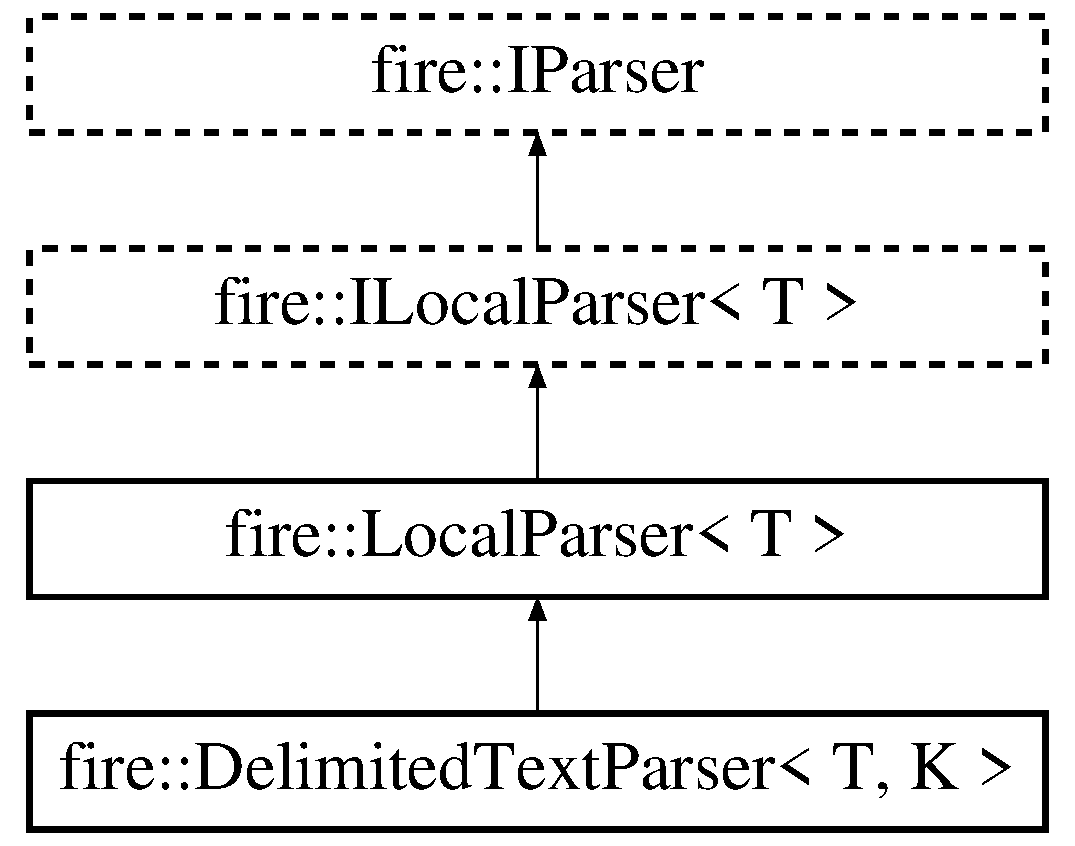
\includegraphics[height=4.000000cm]{a00778}
\end{center}
\end{figure}
\subsection*{Public Member Functions}
\begin{DoxyCompactItemize}
\item 
virtual void \hyperlink{a00778_afcaec6429fdd6e5d53642a32c001ff73}{set\+Source} (const std\+::string \&source)
\item 
virtual void \hyperlink{a00778_abd8929aea06c2dda40256d2e58236650}{parse} ()
\item 
virtual void \hyperlink{a00778_aed4357541f2ff7d46f8846bd07bb3c42}{set\+Source} (const std\+::istream \&source)
\item 
virtual const std\+::string \& \hyperlink{a00778_aedb7fe10911182525a719963b9b56726}{get\+Source} ()
\item 
virtual const std\+::istream \& \hyperlink{a00778_a9bf19a3cc9ae8ac0e6e7a0e7f6212cdc}{get\+Source\+Stream} ()
\item 
virtual std\+::shared\+\_\+ptr$<$ T $>$ \hyperlink{a00778_ab9016cca8e5dca516bb57c6a8e76607a}{get\+Data} ()
\item 
{\footnotesize template$<$$>$ }\\void \hyperlink{a00778_a34fd9ffb0196c612c75b5288ed5e219b}{parse} ()
\item 
{\footnotesize template$<$$>$ }\\void \hyperlink{a00778_ae904e264fe16708b3e434adea59e1b88}{parse} ()
\end{DoxyCompactItemize}
\subsection*{Protected Attributes}
\begin{DoxyCompactItemize}
\item 
std\+::string \hyperlink{a00778_acf921ee916266efe70be5b24bec37fce}{source\+File}
\item 
std\+::shared\+\_\+ptr$<$ T $>$ \hyperlink{a00778_af8f722c7e35378c69e76e4275d384d86}{data}
\end{DoxyCompactItemize}


\subsection{Detailed Description}
\subsubsection*{template$<$typename T$>$\newline
class fire\+::\+Local\+Parser$<$ T $>$}

The Local\+Parser$<$\+T$>$ is a templated parser that provides support for parsing local files of various types based only on the templated type.

This class works through {\itshape Explicit Specialization}, where subclasses are created using concrete types as template arguments instead of through direct inheritance. One important benefit of this approach to the author is that parsing with local files comes uniform and type-\/independent. For example,


\begin{DoxyCode}
LocalParser<UTKAstroNetwork> parser1;
LocalParser<ReacLib> parser2;

\textcolor{comment}{// Other work...}

network = parser1.parse();
rates = parser2.parse();
\end{DoxyCode}


Confer {\itshape C++ Templates\+: The Complete Guide} by Vandervoorde and Josuttis for full details on explicit specialization.

This class always assumes that its source is a file.

F\+I\+X\+M\+E! -\/ Specialization

Subclasses must always be sure that they implement \hyperlink{a00778_abd8929aea06c2dda40256d2e58236650}{parse()} and \hyperlink{a00778_afcaec6429fdd6e5d53642a32c001ff73}{set\+Source()} because default implementations are not provided. 

\subsection{Member Function Documentation}
\mbox{\Hypertarget{a00778_ab9016cca8e5dca516bb57c6a8e76607a}\label{a00778_ab9016cca8e5dca516bb57c6a8e76607a}} 
\index{fire\+::\+Local\+Parser@{fire\+::\+Local\+Parser}!get\+Data@{get\+Data}}
\index{get\+Data@{get\+Data}!fire\+::\+Local\+Parser@{fire\+::\+Local\+Parser}}
\subsubsection{\texorpdfstring{get\+Data()}{getData()}}
{\footnotesize\ttfamily template$<$typename T$>$ \\
virtual std\+::shared\+\_\+ptr$<$T$>$ \hyperlink{a00778}{fire\+::\+Local\+Parser}$<$ T $>$\+::get\+Data (\begin{DoxyParamCaption}{ }\end{DoxyParamCaption})\hspace{0.3cm}{\ttfamily [inline]}, {\ttfamily [virtual]}}

This operation returns a shared pointer to an instance of type T. \begin{DoxyReturn}{Returns}
a shared pointer holding an instance of type T that was parsed from the file. 
\end{DoxyReturn}


Implements \hyperlink{a00762_a0fc1446d106f0ab8daf8744a4bd29a65}{fire\+::\+I\+Local\+Parser$<$ T $>$}.

\mbox{\Hypertarget{a00778_aedb7fe10911182525a719963b9b56726}\label{a00778_aedb7fe10911182525a719963b9b56726}} 
\index{fire\+::\+Local\+Parser@{fire\+::\+Local\+Parser}!get\+Source@{get\+Source}}
\index{get\+Source@{get\+Source}!fire\+::\+Local\+Parser@{fire\+::\+Local\+Parser}}
\subsubsection{\texorpdfstring{get\+Source()}{getSource()}}
{\footnotesize\ttfamily template$<$typename T$>$ \\
virtual const std\+::string\& \hyperlink{a00778}{fire\+::\+Local\+Parser}$<$ T $>$\+::get\+Source (\begin{DoxyParamCaption}{ }\end{DoxyParamCaption})\hspace{0.3cm}{\ttfamily [inline]}, {\ttfamily [virtual]}}

This operation gets the data source for the parser. \begin{DoxyReturn}{Returns}
the name of the source 
\end{DoxyReturn}


Implements \hyperlink{a00770_ab55d2644dfa6d950d1f874e1e02df095}{fire\+::\+I\+Parser}.



Reimplemented in \hyperlink{a00766_ad02c9a530f20a706d7bb2554813e8d3a}{fire\+::\+I\+N\+I\+Property\+Parser}.

\mbox{\Hypertarget{a00778_a9bf19a3cc9ae8ac0e6e7a0e7f6212cdc}\label{a00778_a9bf19a3cc9ae8ac0e6e7a0e7f6212cdc}} 
\index{fire\+::\+Local\+Parser@{fire\+::\+Local\+Parser}!get\+Source\+Stream@{get\+Source\+Stream}}
\index{get\+Source\+Stream@{get\+Source\+Stream}!fire\+::\+Local\+Parser@{fire\+::\+Local\+Parser}}
\subsubsection{\texorpdfstring{get\+Source\+Stream()}{getSourceStream()}}
{\footnotesize\ttfamily template$<$typename T$>$ \\
virtual const std\+::istream\& \hyperlink{a00778}{fire\+::\+Local\+Parser}$<$ T $>$\+::get\+Source\+Stream (\begin{DoxyParamCaption}{ }\end{DoxyParamCaption})\hspace{0.3cm}{\ttfamily [inline]}, {\ttfamily [virtual]}}

This operation gets the data source for the parser as a stream if and only if it was set as such. \begin{DoxyReturn}{Returns}
source the stream of delimited text data 
\end{DoxyReturn}


Implements \hyperlink{a00770_ac94c7a288bf669322b93ba171c43f90e}{fire\+::\+I\+Parser}.

\mbox{\Hypertarget{a00778_a34fd9ffb0196c612c75b5288ed5e219b}\label{a00778_a34fd9ffb0196c612c75b5288ed5e219b}} 
\index{fire\+::\+Local\+Parser@{fire\+::\+Local\+Parser}!parse@{parse}}
\index{parse@{parse}!fire\+::\+Local\+Parser@{fire\+::\+Local\+Parser}}
\subsubsection{\texorpdfstring{parse()}{parse()}\hspace{0.1cm}{\footnotesize\ttfamily [1/3]}}
{\footnotesize\ttfamily template$<$$>$ \\
void \hyperlink{a00778}{fire\+::\+Local\+Parser}$<$ vector$<$ \hyperlink{a00734}{Reaction} $>$ $>$\+::parse (\begin{DoxyParamCaption}{ }\end{DoxyParamCaption})\hspace{0.3cm}{\ttfamily [virtual]}}

This operation parses a file that holds the basic Reaction information for a thermonuclear network. 

Implements \hyperlink{a00770_af36ac6eedd8c27d2f418869193d7d03c}{fire\+::\+I\+Parser}.



Reimplemented in \hyperlink{a00758_a773fa7ed28cb9d8c384ad94bd81fc93f}{fire\+::\+Delimited\+Text\+Parser$<$ T, K $>$}.

\mbox{\Hypertarget{a00778_ae904e264fe16708b3e434adea59e1b88}\label{a00778_ae904e264fe16708b3e434adea59e1b88}} 
\index{fire\+::\+Local\+Parser@{fire\+::\+Local\+Parser}!parse@{parse}}
\index{parse@{parse}!fire\+::\+Local\+Parser@{fire\+::\+Local\+Parser}}
\subsubsection{\texorpdfstring{parse()}{parse()}\hspace{0.1cm}{\footnotesize\ttfamily [2/3]}}
{\footnotesize\ttfamily template$<$$>$ \\
void \hyperlink{a00778}{fire\+::\+Local\+Parser}$<$ std\+::vector$<$ \hyperlink{a00742}{Species} $>$ $>$\+::parse (\begin{DoxyParamCaption}{ }\end{DoxyParamCaption})\hspace{0.3cm}{\ttfamily [virtual]}}

This operation parses a file that holds the basic species information for a thermonuclear network. 

Implements \hyperlink{a00770_af36ac6eedd8c27d2f418869193d7d03c}{fire\+::\+I\+Parser}.



Reimplemented in \hyperlink{a00758_a773fa7ed28cb9d8c384ad94bd81fc93f}{fire\+::\+Delimited\+Text\+Parser$<$ T, K $>$}.

\mbox{\Hypertarget{a00778_abd8929aea06c2dda40256d2e58236650}\label{a00778_abd8929aea06c2dda40256d2e58236650}} 
\index{fire\+::\+Local\+Parser@{fire\+::\+Local\+Parser}!parse@{parse}}
\index{parse@{parse}!fire\+::\+Local\+Parser@{fire\+::\+Local\+Parser}}
\subsubsection{\texorpdfstring{parse()}{parse()}\hspace{0.1cm}{\footnotesize\ttfamily [3/3]}}
{\footnotesize\ttfamily template$<$typename T$>$ \\
virtual void \hyperlink{a00778}{fire\+::\+Local\+Parser}$<$ T $>$\+::parse (\begin{DoxyParamCaption}{ }\end{DoxyParamCaption})\hspace{0.3cm}{\ttfamily [inline]}, {\ttfamily [virtual]}}

This operation directs the parser to parse its source. 

Implements \hyperlink{a00770_af36ac6eedd8c27d2f418869193d7d03c}{fire\+::\+I\+Parser}.



Reimplemented in \hyperlink{a00758_a773fa7ed28cb9d8c384ad94bd81fc93f}{fire\+::\+Delimited\+Text\+Parser$<$ T, K $>$}, \hyperlink{a00758_a686df5548771cae833d5e721442a821a}{fire\+::\+Delimited\+Text\+Parser$<$ T, K $>$}, and \hyperlink{a00766_a31b6bad01e65ed4bb5f1ba297616c641}{fire\+::\+I\+N\+I\+Property\+Parser}.

\mbox{\Hypertarget{a00778_afcaec6429fdd6e5d53642a32c001ff73}\label{a00778_afcaec6429fdd6e5d53642a32c001ff73}} 
\index{fire\+::\+Local\+Parser@{fire\+::\+Local\+Parser}!set\+Source@{set\+Source}}
\index{set\+Source@{set\+Source}!fire\+::\+Local\+Parser@{fire\+::\+Local\+Parser}}
\subsubsection{\texorpdfstring{set\+Source()}{setSource()}\hspace{0.1cm}{\footnotesize\ttfamily [1/2]}}
{\footnotesize\ttfamily template$<$typename T$>$ \\
virtual void \hyperlink{a00778}{fire\+::\+Local\+Parser}$<$ T $>$\+::set\+Source (\begin{DoxyParamCaption}\item[{const std\+::string \&}]{source }\end{DoxyParamCaption})\hspace{0.3cm}{\ttfamily [inline]}, {\ttfamily [virtual]}}

This operation sets the data source for the parser. 
\begin{DoxyParams}{Parameters}
{\em source} & the name of the source that the parser should parse. \\
\hline
\end{DoxyParams}


Implements \hyperlink{a00770_a0dbeff2b9bd8dbfb2aad7a424eef87d1}{fire\+::\+I\+Parser}.



Reimplemented in \hyperlink{a00766_a06793909bc707a69d0c5772b14bc946d}{fire\+::\+I\+N\+I\+Property\+Parser}.

\mbox{\Hypertarget{a00778_aed4357541f2ff7d46f8846bd07bb3c42}\label{a00778_aed4357541f2ff7d46f8846bd07bb3c42}} 
\index{fire\+::\+Local\+Parser@{fire\+::\+Local\+Parser}!set\+Source@{set\+Source}}
\index{set\+Source@{set\+Source}!fire\+::\+Local\+Parser@{fire\+::\+Local\+Parser}}
\subsubsection{\texorpdfstring{set\+Source()}{setSource()}\hspace{0.1cm}{\footnotesize\ttfamily [2/2]}}
{\footnotesize\ttfamily template$<$typename T$>$ \\
virtual void \hyperlink{a00778}{fire\+::\+Local\+Parser}$<$ T $>$\+::set\+Source (\begin{DoxyParamCaption}\item[{const std\+::istream \&}]{source }\end{DoxyParamCaption})\hspace{0.3cm}{\ttfamily [inline]}, {\ttfamily [virtual]}}

This operation sets the data source for the parser using a stream instead of a string. 
\begin{DoxyParams}{Parameters}
{\em source} & the stream of delimited text data \\
\hline
\end{DoxyParams}


Implements \hyperlink{a00770_a7748a633910e9bfc27411d6bd840496b}{fire\+::\+I\+Parser}.



\subsection{Member Data Documentation}
\mbox{\Hypertarget{a00778_af8f722c7e35378c69e76e4275d384d86}\label{a00778_af8f722c7e35378c69e76e4275d384d86}} 
\index{fire\+::\+Local\+Parser@{fire\+::\+Local\+Parser}!data@{data}}
\index{data@{data}!fire\+::\+Local\+Parser@{fire\+::\+Local\+Parser}}
\subsubsection{\texorpdfstring{data}{data}}
{\footnotesize\ttfamily template$<$typename T$>$ \\
std\+::shared\+\_\+ptr$<$T$>$ \hyperlink{a00778}{fire\+::\+Local\+Parser}$<$ T $>$\+::data\hspace{0.3cm}{\ttfamily [protected]}}

The shared pointer to the data set loaded by the \hyperlink{a00778_abd8929aea06c2dda40256d2e58236650}{parse()} operation. \mbox{\Hypertarget{a00778_acf921ee916266efe70be5b24bec37fce}\label{a00778_acf921ee916266efe70be5b24bec37fce}} 
\index{fire\+::\+Local\+Parser@{fire\+::\+Local\+Parser}!source\+File@{source\+File}}
\index{source\+File@{source\+File}!fire\+::\+Local\+Parser@{fire\+::\+Local\+Parser}}
\subsubsection{\texorpdfstring{source\+File}{sourceFile}}
{\footnotesize\ttfamily template$<$typename T$>$ \\
std\+::string \hyperlink{a00778}{fire\+::\+Local\+Parser}$<$ T $>$\+::source\+File\hspace{0.3cm}{\ttfamily [protected]}}

The source file name used if set\+Source(string) is called. 

The documentation for this class was generated from the following file\+:\begin{DoxyCompactItemize}
\item 
Local\+Parser.\+h\end{DoxyCompactItemize}

\hypertarget{a00890}{}\section{C\+Simple\+Ini\+Templ$<$ S\+I\+\_\+\+C\+H\+AR, S\+I\+\_\+\+S\+T\+R\+L\+E\+SS, S\+I\+\_\+\+C\+O\+N\+V\+E\+R\+T\+ER $>$\+:\+:Entry\+:\+:Key\+Order Struct Reference}
\label{a00890}\index{C\+Simple\+Ini\+Templ$<$ S\+I\+\_\+\+C\+H\+A\+R, S\+I\+\_\+\+S\+T\+R\+L\+E\+S\+S, S\+I\+\_\+\+C\+O\+N\+V\+E\+R\+T\+E\+R $>$\+::\+Entry\+::\+Key\+Order@{C\+Simple\+Ini\+Templ$<$ S\+I\+\_\+\+C\+H\+A\+R, S\+I\+\_\+\+S\+T\+R\+L\+E\+S\+S, S\+I\+\_\+\+C\+O\+N\+V\+E\+R\+T\+E\+R $>$\+::\+Entry\+::\+Key\+Order}}


{\ttfamily \#include $<$Simple\+Ini.\+h$>$}

Inheritance diagram for C\+Simple\+Ini\+Templ$<$ S\+I\+\_\+\+C\+H\+AR, S\+I\+\_\+\+S\+T\+R\+L\+E\+SS, S\+I\+\_\+\+C\+O\+N\+V\+E\+R\+T\+ER $>$\+:\+:Entry\+:\+:Key\+Order\+:\begin{figure}[H]
\begin{center}
\leavevmode
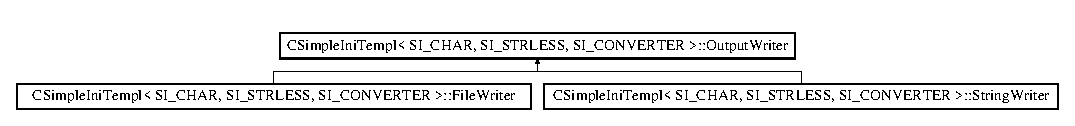
\includegraphics[height=2.000000cm]{a00890}
\end{center}
\end{figure}
\subsection*{Public Member Functions}
\begin{DoxyCompactItemize}
\item 
\mbox{\Hypertarget{a00890_a402ee4ace1311daeaa0eae6c4c83bf87}\label{a00890_a402ee4ace1311daeaa0eae6c4c83bf87}} 
bool {\bfseries operator()} (const \hyperlink{a00886}{Entry} \&lhs, const \hyperlink{a00886}{Entry} \&rhs) const
\end{DoxyCompactItemize}


\subsection{Detailed Description}
\subsubsection*{template$<$class S\+I\+\_\+\+C\+H\+AR, class S\+I\+\_\+\+S\+T\+R\+L\+E\+SS, class S\+I\+\_\+\+C\+O\+N\+V\+E\+R\+T\+ER$>$\newline
struct C\+Simple\+Ini\+Templ$<$ S\+I\+\_\+\+C\+H\+A\+R, S\+I\+\_\+\+S\+T\+R\+L\+E\+S\+S, S\+I\+\_\+\+C\+O\+N\+V\+E\+R\+T\+E\+R $>$\+::\+Entry\+::\+Key\+Order}

Strict less ordering by name of key only 

The documentation for this struct was generated from the following file\+:\begin{DoxyCompactItemize}
\item 
Simple\+Ini.\+h\end{DoxyCompactItemize}

\hypertarget{a00750}{}\section{fire\+:\+:Profile\+Stepper Class Reference}
\label{a00750}\index{fire\+::\+Profile\+Stepper@{fire\+::\+Profile\+Stepper}}


{\ttfamily \#include $<$Profile\+Stepper.\+h$>$}

Inheritance diagram for fire\+:\+:Profile\+Stepper\+:\begin{figure}[H]
\begin{center}
\leavevmode
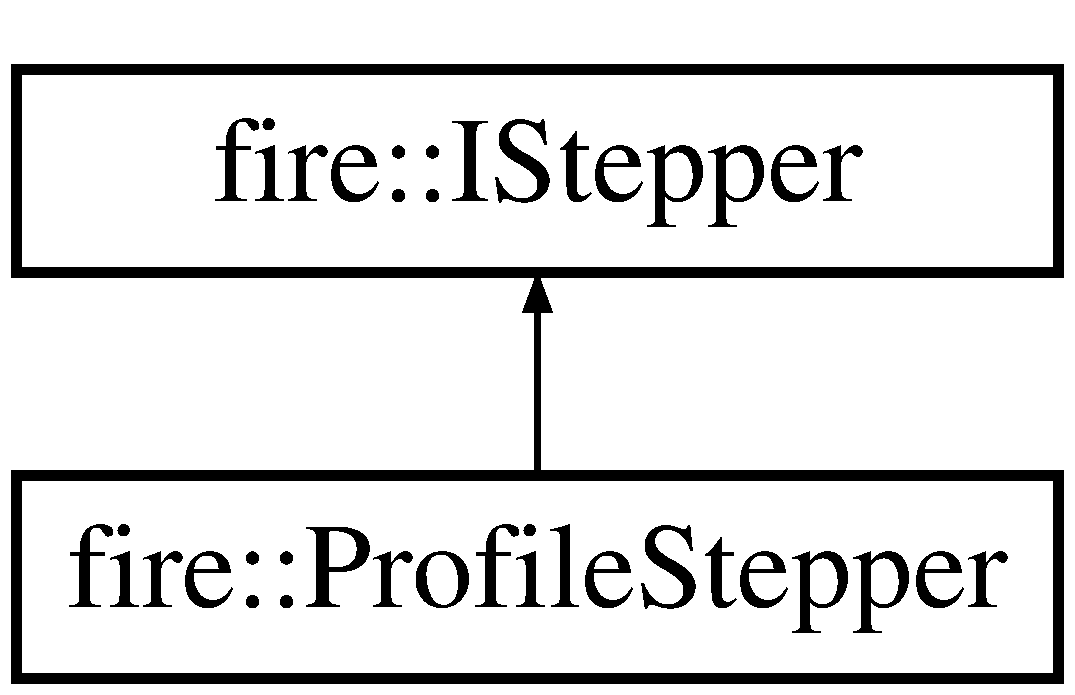
\includegraphics[height=2.000000cm]{a00750}
\end{center}
\end{figure}
\subsection*{Public Member Functions}
\begin{DoxyCompactItemize}
\item 
\hyperlink{a00750_a5bba5babbcb293b5e6a535cc4d06c55f}{Profile\+Stepper} (const std\+::vector$<$ double $>$ \&steps\+List, const std\+::vector$<$ double $>$ \&step\+Size\+List)
\item 
\hyperlink{a00750_a6838143d952dec2519a43c576a1f1546}{$\sim$\+Profile\+Stepper} ()
\item 
virtual double \hyperlink{a00750_a9096ad65a3fcf63678b600cbe0c33961}{get\+Step} ()
\item 
virtual double \hyperlink{a00750_adaa1a23c068977ecc6809dd8eecab49d}{get\+Step\+Size\+At\+Stage} (int i)
\item 
virtual void \hyperlink{a00750_a2c13fd4da5550f1e58df2b54bbfe4c2c}{update\+Step} ()
\item 
virtual void \hyperlink{a00750_adf2f78648d9539282225117c0fd243af}{set\+Initial\+Step} (double initial\+Step)
\item 
virtual double \hyperlink{a00750_af24660fa4bd027f877d5c1bdeb286cf5}{get\+Initial\+Step} ()
\item 
virtual void \hyperlink{a00750_af8203296b4f3bef53bafab7cb654cc97}{set\+Final\+Step} (double \hyperlink{a00750_a4f2347f039417fe9cdd16d3ca74a072d}{final\+Step})
\item 
virtual double \hyperlink{a00750_ae6f257aca7b3bb62a851169a01bcaacf}{get\+Final\+Step} ()
\item 
virtual void \hyperlink{a00750_a55c44fd97d8b6a474243ad0da48b039d}{set\+Initial\+Stepsize} (double step\+Size)
\item 
virtual double \hyperlink{a00750_a86e7035366907a08a36722655746271e}{get\+Initial\+Stepsize} ()
\end{DoxyCompactItemize}
\subsection*{Protected Attributes}
\begin{DoxyCompactItemize}
\item 
const std\+::vector$<$ double $>$ \& \hyperlink{a00750_a4b388e68798f39795386758f85525cf3}{steps}
\item 
const std\+::vector$<$ double $>$ \& \hyperlink{a00750_a3ab053b93662a362fa16147e88a03c22}{step\+Sizes}
\item 
int \hyperlink{a00750_ac3a3c58d7ff087d09ea71f5f33264853}{step\+ID} = 0
\item 
double \hyperlink{a00750_a4f2347f039417fe9cdd16d3ca74a072d}{final\+Step}
\end{DoxyCompactItemize}


\subsection{Detailed Description}
This class is a Stepper that pulls its steps and step sizes from two matching lists. It can be used for restricting the stepping to a pre-\/determined profile, which is useful for coupling and testing. 

\subsection{Constructor \& Destructor Documentation}
\mbox{\Hypertarget{a00750_a5bba5babbcb293b5e6a535cc4d06c55f}\label{a00750_a5bba5babbcb293b5e6a535cc4d06c55f}} 
\index{fire\+::\+Profile\+Stepper@{fire\+::\+Profile\+Stepper}!Profile\+Stepper@{Profile\+Stepper}}
\index{Profile\+Stepper@{Profile\+Stepper}!fire\+::\+Profile\+Stepper@{fire\+::\+Profile\+Stepper}}
\subsubsection{\texorpdfstring{Profile\+Stepper()}{ProfileStepper()}}
{\footnotesize\ttfamily fire\+::\+Profile\+Stepper\+::\+Profile\+Stepper (\begin{DoxyParamCaption}\item[{const std\+::vector$<$ double $>$ \&}]{steps\+List,  }\item[{const std\+::vector$<$ double $>$ \&}]{step\+Size\+List }\end{DoxyParamCaption})\hspace{0.3cm}{\ttfamily [inline]}}

Constructor \mbox{\Hypertarget{a00750_a6838143d952dec2519a43c576a1f1546}\label{a00750_a6838143d952dec2519a43c576a1f1546}} 
\index{fire\+::\+Profile\+Stepper@{fire\+::\+Profile\+Stepper}!````~Profile\+Stepper@{$\sim$\+Profile\+Stepper}}
\index{````~Profile\+Stepper@{$\sim$\+Profile\+Stepper}!fire\+::\+Profile\+Stepper@{fire\+::\+Profile\+Stepper}}
\subsubsection{\texorpdfstring{$\sim$\+Profile\+Stepper()}{~ProfileStepper()}}
{\footnotesize\ttfamily fire\+::\+Profile\+Stepper\+::$\sim$\+Profile\+Stepper (\begin{DoxyParamCaption}{ }\end{DoxyParamCaption})\hspace{0.3cm}{\ttfamily [inline]}}

Destructor 

\subsection{Member Function Documentation}
\mbox{\Hypertarget{a00750_ae6f257aca7b3bb62a851169a01bcaacf}\label{a00750_ae6f257aca7b3bb62a851169a01bcaacf}} 
\index{fire\+::\+Profile\+Stepper@{fire\+::\+Profile\+Stepper}!get\+Final\+Step@{get\+Final\+Step}}
\index{get\+Final\+Step@{get\+Final\+Step}!fire\+::\+Profile\+Stepper@{fire\+::\+Profile\+Stepper}}
\subsubsection{\texorpdfstring{get\+Final\+Step()}{getFinalStep()}}
{\footnotesize\ttfamily virtual double fire\+::\+Profile\+Stepper\+::get\+Final\+Step (\begin{DoxyParamCaption}{ }\end{DoxyParamCaption})\hspace{0.3cm}{\ttfamily [inline]}, {\ttfamily [virtual]}}

This operation returns the final step for the stepper. \begin{DoxyReturn}{Returns}
the final step 
\end{DoxyReturn}


Implements \hyperlink{a00746_ab234d9f032e02668aededf1c22e8c0a9}{fire\+::\+I\+Stepper}.

\mbox{\Hypertarget{a00750_af24660fa4bd027f877d5c1bdeb286cf5}\label{a00750_af24660fa4bd027f877d5c1bdeb286cf5}} 
\index{fire\+::\+Profile\+Stepper@{fire\+::\+Profile\+Stepper}!get\+Initial\+Step@{get\+Initial\+Step}}
\index{get\+Initial\+Step@{get\+Initial\+Step}!fire\+::\+Profile\+Stepper@{fire\+::\+Profile\+Stepper}}
\subsubsection{\texorpdfstring{get\+Initial\+Step()}{getInitialStep()}}
{\footnotesize\ttfamily virtual double fire\+::\+Profile\+Stepper\+::get\+Initial\+Step (\begin{DoxyParamCaption}{ }\end{DoxyParamCaption})\hspace{0.3cm}{\ttfamily [inline]}, {\ttfamily [virtual]}}

This operation returns the initial step for the stepper. \begin{DoxyReturn}{Returns}
the initial step 
\end{DoxyReturn}


Implements \hyperlink{a00746_a49df3a2ac05cebaf2baf387b66d19272}{fire\+::\+I\+Stepper}.

\mbox{\Hypertarget{a00750_a86e7035366907a08a36722655746271e}\label{a00750_a86e7035366907a08a36722655746271e}} 
\index{fire\+::\+Profile\+Stepper@{fire\+::\+Profile\+Stepper}!get\+Initial\+Stepsize@{get\+Initial\+Stepsize}}
\index{get\+Initial\+Stepsize@{get\+Initial\+Stepsize}!fire\+::\+Profile\+Stepper@{fire\+::\+Profile\+Stepper}}
\subsubsection{\texorpdfstring{get\+Initial\+Stepsize()}{getInitialStepsize()}}
{\footnotesize\ttfamily virtual double fire\+::\+Profile\+Stepper\+::get\+Initial\+Stepsize (\begin{DoxyParamCaption}{ }\end{DoxyParamCaption})\hspace{0.3cm}{\ttfamily [inline]}, {\ttfamily [virtual]}}

This operation gets the initial step size for the stepper \begin{DoxyReturn}{Returns}
the initial step size 
\end{DoxyReturn}


Implements \hyperlink{a00746_afb777e62386b25e5a38d59af54972690}{fire\+::\+I\+Stepper}.

\mbox{\Hypertarget{a00750_a9096ad65a3fcf63678b600cbe0c33961}\label{a00750_a9096ad65a3fcf63678b600cbe0c33961}} 
\index{fire\+::\+Profile\+Stepper@{fire\+::\+Profile\+Stepper}!get\+Step@{get\+Step}}
\index{get\+Step@{get\+Step}!fire\+::\+Profile\+Stepper@{fire\+::\+Profile\+Stepper}}
\subsubsection{\texorpdfstring{get\+Step()}{getStep()}}
{\footnotesize\ttfamily virtual double fire\+::\+Profile\+Stepper\+::get\+Step (\begin{DoxyParamCaption}{ }\end{DoxyParamCaption})\hspace{0.3cm}{\ttfamily [inline]}, {\ttfamily [virtual]}}

This operation returns the step value for the current step. \begin{DoxyReturn}{Returns}
the step value 
\end{DoxyReturn}


Implements \hyperlink{a00746_a7f709d1462a2a3b8bd8214cc681ca26e}{fire\+::\+I\+Stepper}.

\mbox{\Hypertarget{a00750_adaa1a23c068977ecc6809dd8eecab49d}\label{a00750_adaa1a23c068977ecc6809dd8eecab49d}} 
\index{fire\+::\+Profile\+Stepper@{fire\+::\+Profile\+Stepper}!get\+Step\+Size\+At\+Stage@{get\+Step\+Size\+At\+Stage}}
\index{get\+Step\+Size\+At\+Stage@{get\+Step\+Size\+At\+Stage}!fire\+::\+Profile\+Stepper@{fire\+::\+Profile\+Stepper}}
\subsubsection{\texorpdfstring{get\+Step\+Size\+At\+Stage()}{getStepSizeAtStage()}}
{\footnotesize\ttfamily virtual double fire\+::\+Profile\+Stepper\+::get\+Step\+Size\+At\+Stage (\begin{DoxyParamCaption}\item[{int}]{i }\end{DoxyParamCaption})\hspace{0.3cm}{\ttfamily [inline]}, {\ttfamily [virtual]}}

This operation returns the step size for the given stage. 
\begin{DoxyParams}{Parameters}
{\em the} & stage of the solver for which the stepsize should be computed \\
\hline
\end{DoxyParams}
\begin{DoxyReturn}{Returns}
the step size 
\end{DoxyReturn}


Implements \hyperlink{a00746_a43027c0c268afcd59db8815c2e2c41ea}{fire\+::\+I\+Stepper}.

\mbox{\Hypertarget{a00750_af8203296b4f3bef53bafab7cb654cc97}\label{a00750_af8203296b4f3bef53bafab7cb654cc97}} 
\index{fire\+::\+Profile\+Stepper@{fire\+::\+Profile\+Stepper}!set\+Final\+Step@{set\+Final\+Step}}
\index{set\+Final\+Step@{set\+Final\+Step}!fire\+::\+Profile\+Stepper@{fire\+::\+Profile\+Stepper}}
\subsubsection{\texorpdfstring{set\+Final\+Step()}{setFinalStep()}}
{\footnotesize\ttfamily virtual void fire\+::\+Profile\+Stepper\+::set\+Final\+Step (\begin{DoxyParamCaption}\item[{double}]{final\+Step }\end{DoxyParamCaption})\hspace{0.3cm}{\ttfamily [inline]}, {\ttfamily [virtual]}}

This operation sets the final step for the stepper. 
\begin{DoxyParams}{Parameters}
{\em final\+Step} & the final step \\
\hline
\end{DoxyParams}


Implements \hyperlink{a00746_add76974a7b6fbbc93916270a376c461e}{fire\+::\+I\+Stepper}.

\mbox{\Hypertarget{a00750_adf2f78648d9539282225117c0fd243af}\label{a00750_adf2f78648d9539282225117c0fd243af}} 
\index{fire\+::\+Profile\+Stepper@{fire\+::\+Profile\+Stepper}!set\+Initial\+Step@{set\+Initial\+Step}}
\index{set\+Initial\+Step@{set\+Initial\+Step}!fire\+::\+Profile\+Stepper@{fire\+::\+Profile\+Stepper}}
\subsubsection{\texorpdfstring{set\+Initial\+Step()}{setInitialStep()}}
{\footnotesize\ttfamily virtual void fire\+::\+Profile\+Stepper\+::set\+Initial\+Step (\begin{DoxyParamCaption}\item[{double}]{initial\+Step }\end{DoxyParamCaption})\hspace{0.3cm}{\ttfamily [inline]}, {\ttfamily [virtual]}}

This operation sets the initial step for the stepper. 
\begin{DoxyParams}{Parameters}
{\em initial\+Step} & the initial step \\
\hline
\end{DoxyParams}


Implements \hyperlink{a00746_a3a5099cd0f3c874e56c33cb8f13b8f3b}{fire\+::\+I\+Stepper}.

\mbox{\Hypertarget{a00750_a55c44fd97d8b6a474243ad0da48b039d}\label{a00750_a55c44fd97d8b6a474243ad0da48b039d}} 
\index{fire\+::\+Profile\+Stepper@{fire\+::\+Profile\+Stepper}!set\+Initial\+Stepsize@{set\+Initial\+Stepsize}}
\index{set\+Initial\+Stepsize@{set\+Initial\+Stepsize}!fire\+::\+Profile\+Stepper@{fire\+::\+Profile\+Stepper}}
\subsubsection{\texorpdfstring{set\+Initial\+Stepsize()}{setInitialStepsize()}}
{\footnotesize\ttfamily virtual void fire\+::\+Profile\+Stepper\+::set\+Initial\+Stepsize (\begin{DoxyParamCaption}\item[{double}]{step\+Size }\end{DoxyParamCaption})\hspace{0.3cm}{\ttfamily [inline]}, {\ttfamily [virtual]}}

This operation sets the initial step size for the stepper 
\begin{DoxyParams}{Parameters}
{\em the} & initial step size \\
\hline
\end{DoxyParams}


Implements \hyperlink{a00746_a69c262f248511efcd271be1724a41ad9}{fire\+::\+I\+Stepper}.

\mbox{\Hypertarget{a00750_a2c13fd4da5550f1e58df2b54bbfe4c2c}\label{a00750_a2c13fd4da5550f1e58df2b54bbfe4c2c}} 
\index{fire\+::\+Profile\+Stepper@{fire\+::\+Profile\+Stepper}!update\+Step@{update\+Step}}
\index{update\+Step@{update\+Step}!fire\+::\+Profile\+Stepper@{fire\+::\+Profile\+Stepper}}
\subsubsection{\texorpdfstring{update\+Step()}{updateStep()}}
{\footnotesize\ttfamily virtual void fire\+::\+Profile\+Stepper\+::update\+Step (\begin{DoxyParamCaption}{ }\end{DoxyParamCaption})\hspace{0.3cm}{\ttfamily [inline]}, {\ttfamily [virtual]}}

This operation replaces the current step and stepsize with the next step and stepsize values. 

Implements \hyperlink{a00746_a44dfccb90ee5ef6e080b54113c215458}{fire\+::\+I\+Stepper}.



\subsection{Member Data Documentation}
\mbox{\Hypertarget{a00750_a4f2347f039417fe9cdd16d3ca74a072d}\label{a00750_a4f2347f039417fe9cdd16d3ca74a072d}} 
\index{fire\+::\+Profile\+Stepper@{fire\+::\+Profile\+Stepper}!final\+Step@{final\+Step}}
\index{final\+Step@{final\+Step}!fire\+::\+Profile\+Stepper@{fire\+::\+Profile\+Stepper}}
\subsubsection{\texorpdfstring{final\+Step}{finalStep}}
{\footnotesize\ttfamily double fire\+::\+Profile\+Stepper\+::final\+Step\hspace{0.3cm}{\ttfamily [protected]}}

The final step value. \mbox{\Hypertarget{a00750_ac3a3c58d7ff087d09ea71f5f33264853}\label{a00750_ac3a3c58d7ff087d09ea71f5f33264853}} 
\index{fire\+::\+Profile\+Stepper@{fire\+::\+Profile\+Stepper}!step\+ID@{step\+ID}}
\index{step\+ID@{step\+ID}!fire\+::\+Profile\+Stepper@{fire\+::\+Profile\+Stepper}}
\subsubsection{\texorpdfstring{step\+ID}{stepID}}
{\footnotesize\ttfamily int fire\+::\+Profile\+Stepper\+::step\+ID = 0\hspace{0.3cm}{\ttfamily [protected]}}

The id number of the current staff \mbox{\Hypertarget{a00750_a4b388e68798f39795386758f85525cf3}\label{a00750_a4b388e68798f39795386758f85525cf3}} 
\index{fire\+::\+Profile\+Stepper@{fire\+::\+Profile\+Stepper}!steps@{steps}}
\index{steps@{steps}!fire\+::\+Profile\+Stepper@{fire\+::\+Profile\+Stepper}}
\subsubsection{\texorpdfstring{steps}{steps}}
{\footnotesize\ttfamily const std\+::vector$<$double$>$\& fire\+::\+Profile\+Stepper\+::steps\hspace{0.3cm}{\ttfamily [protected]}}

The lists of steps \mbox{\Hypertarget{a00750_a3ab053b93662a362fa16147e88a03c22}\label{a00750_a3ab053b93662a362fa16147e88a03c22}} 
\index{fire\+::\+Profile\+Stepper@{fire\+::\+Profile\+Stepper}!step\+Sizes@{step\+Sizes}}
\index{step\+Sizes@{step\+Sizes}!fire\+::\+Profile\+Stepper@{fire\+::\+Profile\+Stepper}}
\subsubsection{\texorpdfstring{step\+Sizes}{stepSizes}}
{\footnotesize\ttfamily const std\+::vector$<$double$>$\& fire\+::\+Profile\+Stepper\+::step\+Sizes\hspace{0.3cm}{\ttfamily [protected]}}

The list of step sizes -\/ the distances between the steps 

The documentation for this class was generated from the following file\+:\begin{DoxyCompactItemize}
\item 
Profile\+Stepper.\+h\end{DoxyCompactItemize}

\hypertarget{a00846}{}\section{fire\+:\+:String\+Caster$<$ bool $>$ Struct Template Reference}
\label{a00846}\index{fire\+::\+String\+Caster$<$ bool $>$@{fire\+::\+String\+Caster$<$ bool $>$}}


{\ttfamily \#include $<$String\+Caster.\+h$>$}

\subsection*{Static Public Member Functions}
\begin{DoxyCompactItemize}
\item 
\mbox{\Hypertarget{a00846_a852e5b28ba000a44312d3ebcb3703e48}\label{a00846_a852e5b28ba000a44312d3ebcb3703e48}} 
static bool {\bfseries cast} (const string \&value)
\end{DoxyCompactItemize}


\subsection{Detailed Description}
\subsubsection*{template$<$$>$\newline
struct fire\+::\+String\+Caster$<$ bool $>$}

Implementation of \hyperlink{a00830}{String\+Caster} for bools 

The documentation for this struct was generated from the following file\+:\begin{DoxyCompactItemize}
\item 
String\+Caster.\+h\end{DoxyCompactItemize}

\hypertarget{a00734}{}\section{fire\+:\+:astrophysics\+:\+:Reaction Struct Reference}
\label{a00734}\index{fire\+::astrophysics\+::\+Reaction@{fire\+::astrophysics\+::\+Reaction}}


{\ttfamily \#include $<$Reaction.\+h$>$}

\subsection*{Public Member Functions}
\begin{DoxyCompactItemize}
\item 
void \hyperlink{a00734_a98b03c550c3926cb5c20f8a27a2ee1ed}{set\+Prefactor} (const double \&rho)
\item 
void \hyperlink{a00734_a671a0560e6843664cdae4d724b8645da}{set\+Rate} (array$<$ double, 6 $>$ temp\+Values)
\item 
void \hyperlink{a00734_a598fe411c64ab247e5d4f299b4a59b70}{set\+Rate} (const double \&temp)
\end{DoxyCompactItemize}
\subsection*{Public Attributes}
\begin{DoxyCompactItemize}
\item 
std\+::string \hyperlink{a00734_abb359091e992ad4cb4cde0faacf6021b}{name}
\item 
int \hyperlink{a00734_ab6d29b5c28ef33ea1d9219b70f02d98a}{reaction\+Group\+Class}
\item 
int \hyperlink{a00734_adb666fe2c511b5a5e86ebcd35ba7faa4}{reaction\+Group\+Member\+Index}
\item 
int \hyperlink{a00734_a581b5410f62a299f2262324d6c0199c7}{reaclib\+Class}
\item 
int \hyperlink{a00734_a86154569e16ef396c93cdf97c5eaf5b7}{num\+Reactants}
\item 
int \hyperlink{a00734_aa59b550e5dbdd34c9c563e7dfc2cbc1e}{num\+Products}
\item 
bool \hyperlink{a00734_a84165249a444a64bdfc41531fbe81cc0}{is\+Electron\+Capture}
\item 
bool \hyperlink{a00734_ae161628da753400b3d2256e2d10a02b9}{is\+Reverse}
\item 
double \hyperlink{a00734_a439daff55fecd97cafc96f204570376a}{statistical\+Factor}
\item 
double \hyperlink{a00734_a07f4db35c5d9bca2d5c5fc8529ec3801}{energy\+Release}
\item 
array$<$ double, 7 $>$ \hyperlink{a00734_aa6265e73f4d2c55441caf95e6eb6e656}{reaclib\+Rate\+Coeff}
\item 
array$<$ int, 4 $>$ \hyperlink{a00734_a74b96d4f5ff99d60adfb88b096a7e256}{reactantZ}
\item 
array$<$ int, 4 $>$ \hyperlink{a00734_a831dcae79d4ed842c9bbdf51ebdd137f}{reactantN}
\item 
array$<$ int, 4 $>$ \hyperlink{a00734_a0586d888e1f60d6371239af888f9158b}{productZ}
\item 
array$<$ int, 4 $>$ \hyperlink{a00734_a81251169f8dd972b6cdc285fbc42c331}{productN}
\item 
array$<$ int, 3 $>$ \hyperlink{a00734_ab13b0133b89c6531a1648b696324d804}{reactants}
\item 
array$<$ int, 3 $>$ \hyperlink{a00734_a5d0e77ebec059081aaafa5ba86df4c88}{products}
\item 
double \hyperlink{a00734_a5033228e6305beb4e8dd717d2f088d99}{prefactor}
\item 
double \hyperlink{a00734_a343553d449e3cca261f8ee166fa6b699}{rate}
\end{DoxyCompactItemize}


\subsection{Detailed Description}
This class represents a reaction, and specifically a nuclear reaction in the astrophysical case. This includes both forward reactions and backward (decay) reactions with one to four reacting bodies.

At the moment, this struct has an extremely bad design. However, it is worth noting that this is significantly better than what is currently used. There are several useful optimizations that will be added in time, such as using the \hyperlink{a00742}{Species} class and creating a new reaction group class. 

\subsection{Member Function Documentation}
\mbox{\Hypertarget{a00734_a98b03c550c3926cb5c20f8a27a2ee1ed}\label{a00734_a98b03c550c3926cb5c20f8a27a2ee1ed}} 
\index{fire\+::astrophysics\+::\+Reaction@{fire\+::astrophysics\+::\+Reaction}!set\+Prefactor@{set\+Prefactor}}
\index{set\+Prefactor@{set\+Prefactor}!fire\+::astrophysics\+::\+Reaction@{fire\+::astrophysics\+::\+Reaction}}
\subsubsection{\texorpdfstring{set\+Prefactor()}{setPrefactor()}}
{\footnotesize\ttfamily void fire\+::astrophysics\+::\+Reaction\+::set\+Prefactor (\begin{DoxyParamCaption}\item[{const double \&}]{rho }\end{DoxyParamCaption})\hspace{0.3cm}{\ttfamily [inline]}}

The statistical prefactor that act as constant multipliers on this reaction. \[ p_s = s\rho^{(n_R -1)}. \] 
\begin{DoxyParams}{Parameters}
{\em rho} & the current density \\
\hline
\end{DoxyParams}
\mbox{\Hypertarget{a00734_a671a0560e6843664cdae4d724b8645da}\label{a00734_a671a0560e6843664cdae4d724b8645da}} 
\index{fire\+::astrophysics\+::\+Reaction@{fire\+::astrophysics\+::\+Reaction}!set\+Rate@{set\+Rate}}
\index{set\+Rate@{set\+Rate}!fire\+::astrophysics\+::\+Reaction@{fire\+::astrophysics\+::\+Reaction}}
\subsubsection{\texorpdfstring{set\+Rate()}{setRate()}\hspace{0.1cm}{\footnotesize\ttfamily [1/2]}}
{\footnotesize\ttfamily void fire\+::astrophysics\+::\+Reaction\+::set\+Rate (\begin{DoxyParamCaption}\item[{array$<$ double, 6 $>$}]{temp\+Values }\end{DoxyParamCaption})\hspace{0.3cm}{\ttfamily [inline]}}

This operation computes and sets the reaction rate. This version is optimized to use pre-\/computed temperature values so that the costly exponentiation does not need to be repeated for each reaction if the temperature doesn\textquotesingle{}t change.

The rate is computed by \[ R = p_s*\sum_k R_k \] where \[p_s\] is the prefactor (based on the statistical prefactor) and \[ R_k = \exp(p_1 + \frac{p_2}{T_9} + \frac{p_3}{T_9^{1/3}} + p_{4}T_9^{1/3} + p_{5}T_9 + p_{6}T_9^{5/3} + p_{7}\ln T_9). \]

$T_9$ is the the temperature in units of $10^9$ Kelvin. Note that p1 = reaclib\+Rate\+Coeff\mbox{[}0\mbox{]} since C++ is a zero-\/indexed language.

In general k may be greater than 1 in the summation for the rate, but in this work k = 1 and \[R = R_k\].

See\+: \char`\"{}\+Stars and Stellar Processes\char`\"{}, Mike Guidry, to be published Cambridge University Press.


\begin{DoxyParams}{Parameters}
{\em temp\+Values} & An array of all six temperature values used to compute the rate. \\
\hline
\end{DoxyParams}
\mbox{\Hypertarget{a00734_a598fe411c64ab247e5d4f299b4a59b70}\label{a00734_a598fe411c64ab247e5d4f299b4a59b70}} 
\index{fire\+::astrophysics\+::\+Reaction@{fire\+::astrophysics\+::\+Reaction}!set\+Rate@{set\+Rate}}
\index{set\+Rate@{set\+Rate}!fire\+::astrophysics\+::\+Reaction@{fire\+::astrophysics\+::\+Reaction}}
\subsubsection{\texorpdfstring{set\+Rate()}{setRate()}\hspace{0.1cm}{\footnotesize\ttfamily [2/2]}}
{\footnotesize\ttfamily void fire\+::astrophysics\+::\+Reaction\+::set\+Rate (\begin{DoxyParamCaption}\item[{const double \&}]{temp }\end{DoxyParamCaption})\hspace{0.3cm}{\ttfamily [inline]}}

This operation computes and sets the reaction rate. This version will use the provided temperature to compute all of the temperature coefficients. See the other version of this function for a more efficient version (which this function actually calls).

The rate is computed by \[ R = p_s*\sum_k R_k \] where \[p_s\] is the prefactor (based on the statistical prefactor) and \[ R_k = \exp(p_1 + \frac{p_2}{T_9} + \frac{p_3}{T_9^{1/3}} + p_{4}T_9^{1/3} + p_{5}T_9 + p_{6}T_9^{5/3} + p_{7}\ln T_9). \]

$T_9$ is the the temperature in units of $10^9$ Kelvin. Note that p1 = reaclib\+Rate\+Coeff\mbox{[}0\mbox{]} since C++ is a zero-\/indexed language.

In general k may be greater than 1 in the summation for the rate, but in this work k = 1 and \[R = R_k\].

See\+: \char`\"{}\+Stars and Stellar Processes\char`\"{}, Mike Guidry, to be published Cambridge University Press.


\begin{DoxyParams}{Parameters}
{\em temp} & the temperature \\
\hline
\end{DoxyParams}


\subsection{Member Data Documentation}
\mbox{\Hypertarget{a00734_a07f4db35c5d9bca2d5c5fc8529ec3801}\label{a00734_a07f4db35c5d9bca2d5c5fc8529ec3801}} 
\index{fire\+::astrophysics\+::\+Reaction@{fire\+::astrophysics\+::\+Reaction}!energy\+Release@{energy\+Release}}
\index{energy\+Release@{energy\+Release}!fire\+::astrophysics\+::\+Reaction@{fire\+::astrophysics\+::\+Reaction}}
\subsubsection{\texorpdfstring{energy\+Release}{energyRelease}}
{\footnotesize\ttfamily double fire\+::astrophysics\+::\+Reaction\+::energy\+Release}

The energy released by this reaction in electron volts. \mbox{\Hypertarget{a00734_a84165249a444a64bdfc41531fbe81cc0}\label{a00734_a84165249a444a64bdfc41531fbe81cc0}} 
\index{fire\+::astrophysics\+::\+Reaction@{fire\+::astrophysics\+::\+Reaction}!is\+Electron\+Capture@{is\+Electron\+Capture}}
\index{is\+Electron\+Capture@{is\+Electron\+Capture}!fire\+::astrophysics\+::\+Reaction@{fire\+::astrophysics\+::\+Reaction}}
\subsubsection{\texorpdfstring{is\+Electron\+Capture}{isElectronCapture}}
{\footnotesize\ttfamily bool fire\+::astrophysics\+::\+Reaction\+::is\+Electron\+Capture}

This is flag that designates whether or not the reaction captures an electron. \mbox{\Hypertarget{a00734_ae161628da753400b3d2256e2d10a02b9}\label{a00734_ae161628da753400b3d2256e2d10a02b9}} 
\index{fire\+::astrophysics\+::\+Reaction@{fire\+::astrophysics\+::\+Reaction}!is\+Reverse@{is\+Reverse}}
\index{is\+Reverse@{is\+Reverse}!fire\+::astrophysics\+::\+Reaction@{fire\+::astrophysics\+::\+Reaction}}
\subsubsection{\texorpdfstring{is\+Reverse}{isReverse}}
{\footnotesize\ttfamily bool fire\+::astrophysics\+::\+Reaction\+::is\+Reverse}

True if this reaction is a reverse reaction.

A\+SK M\+I\+K\+E! Why is this set to false by in F\+E\+RN\textquotesingle{}s load\+Reactions operation? \mbox{\Hypertarget{a00734_abb359091e992ad4cb4cde0faacf6021b}\label{a00734_abb359091e992ad4cb4cde0faacf6021b}} 
\index{fire\+::astrophysics\+::\+Reaction@{fire\+::astrophysics\+::\+Reaction}!name@{name}}
\index{name@{name}!fire\+::astrophysics\+::\+Reaction@{fire\+::astrophysics\+::\+Reaction}}
\subsubsection{\texorpdfstring{name}{name}}
{\footnotesize\ttfamily std\+::string fire\+::astrophysics\+::\+Reaction\+::name}

The name, or label, for the reaction. This should be of the form\+: \char`\"{}he4+he4+he4-\/-\/$>$c12\char`\"{} \mbox{\Hypertarget{a00734_aa59b550e5dbdd34c9c563e7dfc2cbc1e}\label{a00734_aa59b550e5dbdd34c9c563e7dfc2cbc1e}} 
\index{fire\+::astrophysics\+::\+Reaction@{fire\+::astrophysics\+::\+Reaction}!num\+Products@{num\+Products}}
\index{num\+Products@{num\+Products}!fire\+::astrophysics\+::\+Reaction@{fire\+::astrophysics\+::\+Reaction}}
\subsubsection{\texorpdfstring{num\+Products}{numProducts}}
{\footnotesize\ttfamily int fire\+::astrophysics\+::\+Reaction\+::num\+Products}

The number of products produced as a result of the reaction. \mbox{\Hypertarget{a00734_a86154569e16ef396c93cdf97c5eaf5b7}\label{a00734_a86154569e16ef396c93cdf97c5eaf5b7}} 
\index{fire\+::astrophysics\+::\+Reaction@{fire\+::astrophysics\+::\+Reaction}!num\+Reactants@{num\+Reactants}}
\index{num\+Reactants@{num\+Reactants}!fire\+::astrophysics\+::\+Reaction@{fire\+::astrophysics\+::\+Reaction}}
\subsubsection{\texorpdfstring{num\+Reactants}{numReactants}}
{\footnotesize\ttfamily int fire\+::astrophysics\+::\+Reaction\+::num\+Reactants}

The number of species in this reaction. \mbox{\Hypertarget{a00734_a5033228e6305beb4e8dd717d2f088d99}\label{a00734_a5033228e6305beb4e8dd717d2f088d99}} 
\index{fire\+::astrophysics\+::\+Reaction@{fire\+::astrophysics\+::\+Reaction}!prefactor@{prefactor}}
\index{prefactor@{prefactor}!fire\+::astrophysics\+::\+Reaction@{fire\+::astrophysics\+::\+Reaction}}
\subsubsection{\texorpdfstring{prefactor}{prefactor}}
{\footnotesize\ttfamily double fire\+::astrophysics\+::\+Reaction\+::prefactor}

The statistical prefactor that act as constant multipliers on this reaction. \[ p_s = s\rho^{(n_R -1)}. \] 
\begin{DoxyParams}{Parameters}
{\em the} & current density \\
\hline
\end{DoxyParams}
\mbox{\Hypertarget{a00734_a81251169f8dd972b6cdc285fbc42c331}\label{a00734_a81251169f8dd972b6cdc285fbc42c331}} 
\index{fire\+::astrophysics\+::\+Reaction@{fire\+::astrophysics\+::\+Reaction}!productN@{productN}}
\index{productN@{productN}!fire\+::astrophysics\+::\+Reaction@{fire\+::astrophysics\+::\+Reaction}}
\subsubsection{\texorpdfstring{productN}{productN}}
{\footnotesize\ttfamily array$<$int, 4$>$ fire\+::astrophysics\+::\+Reaction\+::productN}

The array of neutron numbers for the products in this reaction. \mbox{\Hypertarget{a00734_a5d0e77ebec059081aaafa5ba86df4c88}\label{a00734_a5d0e77ebec059081aaafa5ba86df4c88}} 
\index{fire\+::astrophysics\+::\+Reaction@{fire\+::astrophysics\+::\+Reaction}!products@{products}}
\index{products@{products}!fire\+::astrophysics\+::\+Reaction@{fire\+::astrophysics\+::\+Reaction}}
\subsubsection{\texorpdfstring{products}{products}}
{\footnotesize\ttfamily array$<$int, 3$>$ fire\+::astrophysics\+::\+Reaction\+::products}

The array of products to add to reac\+Vector.

No idea. A\+SK M\+I\+K\+E! This is used by the partial equilibrium code and may be useless for now. \mbox{\Hypertarget{a00734_a0586d888e1f60d6371239af888f9158b}\label{a00734_a0586d888e1f60d6371239af888f9158b}} 
\index{fire\+::astrophysics\+::\+Reaction@{fire\+::astrophysics\+::\+Reaction}!productZ@{productZ}}
\index{productZ@{productZ}!fire\+::astrophysics\+::\+Reaction@{fire\+::astrophysics\+::\+Reaction}}
\subsubsection{\texorpdfstring{productZ}{productZ}}
{\footnotesize\ttfamily array$<$int, 4$>$ fire\+::astrophysics\+::\+Reaction\+::productZ}

The array of atomic numbers for the products in this reaction. \mbox{\Hypertarget{a00734_a343553d449e3cca261f8ee166fa6b699}\label{a00734_a343553d449e3cca261f8ee166fa6b699}} 
\index{fire\+::astrophysics\+::\+Reaction@{fire\+::astrophysics\+::\+Reaction}!rate@{rate}}
\index{rate@{rate}!fire\+::astrophysics\+::\+Reaction@{fire\+::astrophysics\+::\+Reaction}}
\subsubsection{\texorpdfstring{rate}{rate}}
{\footnotesize\ttfamily double fire\+::astrophysics\+::\+Reaction\+::rate}

The reaction rate as described in \hyperlink{a00734_a671a0560e6843664cdae4d724b8645da}{set\+Rate()}. \mbox{\Hypertarget{a00734_a581b5410f62a299f2262324d6c0199c7}\label{a00734_a581b5410f62a299f2262324d6c0199c7}} 
\index{fire\+::astrophysics\+::\+Reaction@{fire\+::astrophysics\+::\+Reaction}!reaclib\+Class@{reaclib\+Class}}
\index{reaclib\+Class@{reaclib\+Class}!fire\+::astrophysics\+::\+Reaction@{fire\+::astrophysics\+::\+Reaction}}
\subsubsection{\texorpdfstring{reaclib\+Class}{reaclibClass}}
{\footnotesize\ttfamily int fire\+::astrophysics\+::\+Reaction\+::reaclib\+Class}

The class of this reaction in the R\+E\+A\+C\+L\+IB rate library. \mbox{\Hypertarget{a00734_aa6265e73f4d2c55441caf95e6eb6e656}\label{a00734_aa6265e73f4d2c55441caf95e6eb6e656}} 
\index{fire\+::astrophysics\+::\+Reaction@{fire\+::astrophysics\+::\+Reaction}!reaclib\+Rate\+Coeff@{reaclib\+Rate\+Coeff}}
\index{reaclib\+Rate\+Coeff@{reaclib\+Rate\+Coeff}!fire\+::astrophysics\+::\+Reaction@{fire\+::astrophysics\+::\+Reaction}}
\subsubsection{\texorpdfstring{reaclib\+Rate\+Coeff}{reaclibRateCoeff}}
{\footnotesize\ttfamily array$<$double,7$>$ fire\+::astrophysics\+::\+Reaction\+::reaclib\+Rate\+Coeff}

The array of R\+E\+A\+C\+L\+IB p-\/coefficients used in the parameterized computation of the rate. The rate is computed by \[ R = p_s*\sum_k R_k \] where \[p_s\] is the prefactor (based on the statistical prefactor) and \[ R_k = \exp(p_1 + \frac{p_2}{T_9} + \frac{p_3}{T_9^{1/3}} + p_{4}T_9^{1/3} + p_{5}T_9 + p_{6}T_9^{5/3} + p_{7}\ln T_9). \]

$T_9$ is the the temperature in units of $10^9$ Kelvin. Note that p1 = reaclib\+Rate\+Coeff\mbox{[}0\mbox{]} since C++ is a zero-\/indexed language.

In general k may be greater than 1 in the summation for the rate, but in this work k = 1 and \[R = R_k\].

See\+: \char`\"{}\+Stars and Stellar Processes\char`\"{}, Mike Guidry, to be published Cambridge University Press. \mbox{\Hypertarget{a00734_a831dcae79d4ed842c9bbdf51ebdd137f}\label{a00734_a831dcae79d4ed842c9bbdf51ebdd137f}} 
\index{fire\+::astrophysics\+::\+Reaction@{fire\+::astrophysics\+::\+Reaction}!reactantN@{reactantN}}
\index{reactantN@{reactantN}!fire\+::astrophysics\+::\+Reaction@{fire\+::astrophysics\+::\+Reaction}}
\subsubsection{\texorpdfstring{reactantN}{reactantN}}
{\footnotesize\ttfamily array$<$int, 4$>$ fire\+::astrophysics\+::\+Reaction\+::reactantN}

The array of neutron numbers for the reactants in this reaction. \mbox{\Hypertarget{a00734_ab13b0133b89c6531a1648b696324d804}\label{a00734_ab13b0133b89c6531a1648b696324d804}} 
\index{fire\+::astrophysics\+::\+Reaction@{fire\+::astrophysics\+::\+Reaction}!reactants@{reactants}}
\index{reactants@{reactants}!fire\+::astrophysics\+::\+Reaction@{fire\+::astrophysics\+::\+Reaction}}
\subsubsection{\texorpdfstring{reactants}{reactants}}
{\footnotesize\ttfamily array$<$int, 3$>$ fire\+::astrophysics\+::\+Reaction\+::reactants}

The array of reactants to subtract from reac\+Vector.

No idea. A\+SK M\+I\+K\+E! This is used by the partial equilibrium code and may be useless for now. \mbox{\Hypertarget{a00734_a74b96d4f5ff99d60adfb88b096a7e256}\label{a00734_a74b96d4f5ff99d60adfb88b096a7e256}} 
\index{fire\+::astrophysics\+::\+Reaction@{fire\+::astrophysics\+::\+Reaction}!reactantZ@{reactantZ}}
\index{reactantZ@{reactantZ}!fire\+::astrophysics\+::\+Reaction@{fire\+::astrophysics\+::\+Reaction}}
\subsubsection{\texorpdfstring{reactantZ}{reactantZ}}
{\footnotesize\ttfamily array$<$int, 4$>$ fire\+::astrophysics\+::\+Reaction\+::reactantZ}

The array of atomic numbers for the reactants in this reaction. \mbox{\Hypertarget{a00734_ab6d29b5c28ef33ea1d9219b70f02d98a}\label{a00734_ab6d29b5c28ef33ea1d9219b70f02d98a}} 
\index{fire\+::astrophysics\+::\+Reaction@{fire\+::astrophysics\+::\+Reaction}!reaction\+Group\+Class@{reaction\+Group\+Class}}
\index{reaction\+Group\+Class@{reaction\+Group\+Class}!fire\+::astrophysics\+::\+Reaction@{fire\+::astrophysics\+::\+Reaction}}
\subsubsection{\texorpdfstring{reaction\+Group\+Class}{reactionGroupClass}}
{\footnotesize\ttfamily int fire\+::astrophysics\+::\+Reaction\+::reaction\+Group\+Class}

The class of this reaction within its reaction group. \mbox{\Hypertarget{a00734_adb666fe2c511b5a5e86ebcd35ba7faa4}\label{a00734_adb666fe2c511b5a5e86ebcd35ba7faa4}} 
\index{fire\+::astrophysics\+::\+Reaction@{fire\+::astrophysics\+::\+Reaction}!reaction\+Group\+Member\+Index@{reaction\+Group\+Member\+Index}}
\index{reaction\+Group\+Member\+Index@{reaction\+Group\+Member\+Index}!fire\+::astrophysics\+::\+Reaction@{fire\+::astrophysics\+::\+Reaction}}
\subsubsection{\texorpdfstring{reaction\+Group\+Member\+Index}{reactionGroupMemberIndex}}
{\footnotesize\ttfamily int fire\+::astrophysics\+::\+Reaction\+::reaction\+Group\+Member\+Index}

The index of this reaction within the reaction group. \mbox{\Hypertarget{a00734_a439daff55fecd97cafc96f204570376a}\label{a00734_a439daff55fecd97cafc96f204570376a}} 
\index{fire\+::astrophysics\+::\+Reaction@{fire\+::astrophysics\+::\+Reaction}!statistical\+Factor@{statistical\+Factor}}
\index{statistical\+Factor@{statistical\+Factor}!fire\+::astrophysics\+::\+Reaction@{fire\+::astrophysics\+::\+Reaction}}
\subsubsection{\texorpdfstring{statistical\+Factor}{statisticalFactor}}
{\footnotesize\ttfamily double fire\+::astrophysics\+::\+Reaction\+::statistical\+Factor}

A statistical factor associated with this reaction that avoids double counting. It also accounts for the sign needed to designate whether or not the population is depleting or increasing. 

The documentation for this struct was generated from the following file\+:\begin{DoxyCompactItemize}
\item 
Reaction.\+h\end{DoxyCompactItemize}

\hypertarget{a00738}{}\section{fire\+:\+:astrophysics\+:\+:Reaction\+Network Class Reference}
\label{a00738}\index{fire\+::astrophysics\+::\+Reaction\+Network@{fire\+::astrophysics\+::\+Reaction\+Network}}


{\ttfamily \#include $<$Reaction\+Network.\+h$>$}

\subsection*{Public Member Functions}
\begin{DoxyCompactItemize}
\item 
\mbox{\Hypertarget{a00738_a66db1b9f2e597f21bce7bcb88b1fbf8f}\label{a00738_a66db1b9f2e597f21bce7bcb88b1fbf8f}} 
double \& {\bfseries operator()} (int i)
\item 
void \hyperlink{a00738_ab4713cafb974ca41bf6a55619e9fd875}{set\+Properties} (const map$<$ string, string $>$ \&props)
\item 
void \hyperlink{a00738_aa9b4de0566ab0b0f148677d8b97e8c49}{load} ()
\item 
void \hyperlink{a00738_aa0c06237ae72e698aee9cf72d0032fd8}{build\+Flux\+Maps} ()
\item 
void \hyperlink{a00738_ac5b97490e667b011b5e2bea92e16f8b7}{compute\+Prefactors} (const double \&rho)
\item 
void \hyperlink{a00738_a3b1fee4e28576c677d7b852e91c6fa98}{compute\+Rates} (const double \&temp)
\item 
void \hyperlink{a00738_a35a05489358c8e1017bbebb75a9c0114}{compute\+Fluxes} ()
\end{DoxyCompactItemize}
\subsection*{Public Attributes}
\begin{DoxyCompactItemize}
\item 
int \hyperlink{a00738_a17ffe8399181590d59d3d339ce867709}{num\+Species}
\item 
int \hyperlink{a00738_ade8f4d9aa1524cbc45809e7943725d59}{num\+Reactions}
\item 
int \hyperlink{a00738_a91f7685b58b70eca227a098717dfe2c5}{num\+Reaction\+Groups}
\item 
double \hyperlink{a00738_ad3d95ecac758ca7efce6376904455123}{mass\+Tol}
\item 
double \hyperlink{a00738_a0bb068c675589e1ad767c1faf2165ed7}{flux\+Frac}
\item 
string \hyperlink{a00738_abcc4209749ecd64d0ab9621210536ade}{network\+File\+Name}
\item 
string \hyperlink{a00738_abb5fbb289b2e40d3b3dcb3695696e2c2}{rate\+File\+Name}
\item 
shared\+\_\+ptr$<$ vector$<$ \hyperlink{a00742}{Species} $>$ $>$ \hyperlink{a00738_ac3811889f4866a29a49ce3a8d0e80cad}{species}
\item 
shared\+\_\+ptr$<$ vector$<$ \hyperlink{a00734}{Reaction} $>$ $>$ \hyperlink{a00738_a32964b6f6a9cb312e722c1478167b7f0}{reactions}
\item 
vector$<$ double $>$ \hyperlink{a00738_af3aa4184f759b2a8babf765667aa6604}{f\+Plus\+Map}
\item 
vector$<$ double $>$ \hyperlink{a00738_a9065be108e95b1604b0d53e2080f0b57}{f\+Minus\+Map}
\item 
vector$<$ double $>$ \hyperlink{a00738_aca9928041359ecf555a63e4f58e80164}{f\+Plus\+Factors}
\item 
vector$<$ double $>$ \hyperlink{a00738_a3aff20108c80e14f9f4d526a08af49de}{f\+Minus\+Factors}
\item 
vector$<$ unsigned short $>$ \hyperlink{a00738_a6682680b1f2975fa8dc1288d3c463693}{f\+Plus\+Maximums}
\item 
vector$<$ unsigned short $>$ \hyperlink{a00738_a4ea51dc9d41bf555592f93bb237e0440}{f\+Minus\+Maximums}
\item 
\mbox{\Hypertarget{a00738_a9309d86802802f33350fbd4fd679fc2b}\label{a00738_a9309d86802802f33350fbd4fd679fc2b}} 
int {\bfseries num\+F\+Plus}
\item 
\mbox{\Hypertarget{a00738_aec06a5e98ef60a1572072c3ad3fa7722}\label{a00738_aec06a5e98ef60a1572072c3ad3fa7722}} 
int {\bfseries num\+F\+Minus}
\end{DoxyCompactItemize}


\subsection{Detailed Description}
This class collects all of the information about a thermonuclear reaction network for astrophysical systems. It includes all species and reaction information and other stateful variable.

The design of this class is not ideal because it exposes public members variables. This design is still an advancement over the original design in F\+E\+RN and is good enough for now. We\textquotesingle{}ll improve it later. 

\subsection{Member Function Documentation}
\mbox{\Hypertarget{a00738_aa0c06237ae72e698aee9cf72d0032fd8}\label{a00738_aa0c06237ae72e698aee9cf72d0032fd8}} 
\index{fire\+::astrophysics\+::\+Reaction\+Network@{fire\+::astrophysics\+::\+Reaction\+Network}!build\+Flux\+Maps@{build\+Flux\+Maps}}
\index{build\+Flux\+Maps@{build\+Flux\+Maps}!fire\+::astrophysics\+::\+Reaction\+Network@{fire\+::astrophysics\+::\+Reaction\+Network}}
\subsubsection{\texorpdfstring{build\+Flux\+Maps()}{buildFluxMaps()}}
{\footnotesize\ttfamily void fire\+::astrophysics\+::\+Reaction\+Network\+::build\+Flux\+Maps (\begin{DoxyParamCaption}{ }\end{DoxyParamCaption})\hspace{0.3cm}{\ttfamily [inline]}}

This operation builds the \char`\"{}flux maps\char`\"{} that map the contributions of each reaction for each species in the network.

This function was originally written as part of the F\+E\+RN code and desperately needs to be refactored. It is has been adapted to use the \hyperlink{a00742}{Species} and \hyperlink{a00734}{Reaction} classes in Fire, but still contains a number of old constructs that have poor performance implications. Likewise, it lacks a sophisticated view of data structures that could greatly increase its speed. It is fine for now because ultimately the formation of the flux maps and numerical prefactors on the R\+HS take up an extremely small amount of computational time compared to the rest of the integration since they are only computed once on initialization of the network. \mbox{\Hypertarget{a00738_a35a05489358c8e1017bbebb75a9c0114}\label{a00738_a35a05489358c8e1017bbebb75a9c0114}} 
\index{fire\+::astrophysics\+::\+Reaction\+Network@{fire\+::astrophysics\+::\+Reaction\+Network}!compute\+Fluxes@{compute\+Fluxes}}
\index{compute\+Fluxes@{compute\+Fluxes}!fire\+::astrophysics\+::\+Reaction\+Network@{fire\+::astrophysics\+::\+Reaction\+Network}}
\subsubsection{\texorpdfstring{compute\+Fluxes()}{computeFluxes()}}
{\footnotesize\ttfamily void fire\+::astrophysics\+::\+Reaction\+Network\+::compute\+Fluxes (\begin{DoxyParamCaption}{ }\end{DoxyParamCaption})\hspace{0.3cm}{\ttfamily [inline]}}

This operation computes the fluxes for the species in the network under the given conditions. The fluxes are stored in the flux member variable on the species itself. \mbox{\Hypertarget{a00738_ac5b97490e667b011b5e2bea92e16f8b7}\label{a00738_ac5b97490e667b011b5e2bea92e16f8b7}} 
\index{fire\+::astrophysics\+::\+Reaction\+Network@{fire\+::astrophysics\+::\+Reaction\+Network}!compute\+Prefactors@{compute\+Prefactors}}
\index{compute\+Prefactors@{compute\+Prefactors}!fire\+::astrophysics\+::\+Reaction\+Network@{fire\+::astrophysics\+::\+Reaction\+Network}}
\subsubsection{\texorpdfstring{compute\+Prefactors()}{computePrefactors()}}
{\footnotesize\ttfamily void fire\+::astrophysics\+::\+Reaction\+Network\+::compute\+Prefactors (\begin{DoxyParamCaption}\item[{const double \&}]{rho }\end{DoxyParamCaption})\hspace{0.3cm}{\ttfamily [inline]}}

This function computes the prefactors for the reaction rates. It is primarily a convenience function for configuring the reactions. The prefactors are stored in the reactions themselves. 
\begin{DoxyParams}{Parameters}
{\em rho} & the current density in units of g/m$^\wedge$3. \\
\hline
\end{DoxyParams}
\mbox{\Hypertarget{a00738_a3b1fee4e28576c677d7b852e91c6fa98}\label{a00738_a3b1fee4e28576c677d7b852e91c6fa98}} 
\index{fire\+::astrophysics\+::\+Reaction\+Network@{fire\+::astrophysics\+::\+Reaction\+Network}!compute\+Rates@{compute\+Rates}}
\index{compute\+Rates@{compute\+Rates}!fire\+::astrophysics\+::\+Reaction\+Network@{fire\+::astrophysics\+::\+Reaction\+Network}}
\subsubsection{\texorpdfstring{compute\+Rates()}{computeRates()}}
{\footnotesize\ttfamily void fire\+::astrophysics\+::\+Reaction\+Network\+::compute\+Rates (\begin{DoxyParamCaption}\item[{const double \&}]{temp }\end{DoxyParamCaption})\hspace{0.3cm}{\ttfamily [inline]}}

This function computers the reaction rates. It is primarily a convenience function for configuring the reactions. The rates are stored in the rate member variable on the reaction itself. 
\begin{DoxyParams}{Parameters}
{\em temp} & the current temperature in units of 10$^\wedge$9 Kelvin. \\
\hline
\end{DoxyParams}
\mbox{\Hypertarget{a00738_aa9b4de0566ab0b0f148677d8b97e8c49}\label{a00738_aa9b4de0566ab0b0f148677d8b97e8c49}} 
\index{fire\+::astrophysics\+::\+Reaction\+Network@{fire\+::astrophysics\+::\+Reaction\+Network}!load@{load}}
\index{load@{load}!fire\+::astrophysics\+::\+Reaction\+Network@{fire\+::astrophysics\+::\+Reaction\+Network}}
\subsubsection{\texorpdfstring{load()}{load()}}
{\footnotesize\ttfamily void fire\+::astrophysics\+::\+Reaction\+Network\+::load (\begin{DoxyParamCaption}{ }\end{DoxyParamCaption})\hspace{0.3cm}{\ttfamily [inline]}}

This operations directs the Network to load the species and reactions from the files provided in the properties list. \mbox{\Hypertarget{a00738_ab4713cafb974ca41bf6a55619e9fd875}\label{a00738_ab4713cafb974ca41bf6a55619e9fd875}} 
\index{fire\+::astrophysics\+::\+Reaction\+Network@{fire\+::astrophysics\+::\+Reaction\+Network}!set\+Properties@{set\+Properties}}
\index{set\+Properties@{set\+Properties}!fire\+::astrophysics\+::\+Reaction\+Network@{fire\+::astrophysics\+::\+Reaction\+Network}}
\subsubsection{\texorpdfstring{set\+Properties()}{setProperties()}}
{\footnotesize\ttfamily void fire\+::astrophysics\+::\+Reaction\+Network\+::set\+Properties (\begin{DoxyParamCaption}\item[{const map$<$ string, string $>$ \&}]{props }\end{DoxyParamCaption})\hspace{0.3cm}{\ttfamily [inline]}}

This operation sets the properties of the network from a map. It is designed to work with property blocks pulled from I\+NI files. It expects the following keys to have values in the map and accepts the default if they do not\+: num\+Species num\+Reactions num\+Reaction\+Groups mass\+Tol flux\+Frac network\+File rate\+File 
\begin{DoxyParams}{Parameters}
{\em props} & the property map \\
\hline
\end{DoxyParams}


\subsection{Member Data Documentation}
\mbox{\Hypertarget{a00738_a0bb068c675589e1ad767c1faf2165ed7}\label{a00738_a0bb068c675589e1ad767c1faf2165ed7}} 
\index{fire\+::astrophysics\+::\+Reaction\+Network@{fire\+::astrophysics\+::\+Reaction\+Network}!flux\+Frac@{flux\+Frac}}
\index{flux\+Frac@{flux\+Frac}!fire\+::astrophysics\+::\+Reaction\+Network@{fire\+::astrophysics\+::\+Reaction\+Network}}
\subsubsection{\texorpdfstring{flux\+Frac}{fluxFrac}}
{\footnotesize\ttfamily double fire\+::astrophysics\+::\+Reaction\+Network\+::flux\+Frac}

A tunable parameter to limit the integration step size based solely on the flux \mbox{\Hypertarget{a00738_a3aff20108c80e14f9f4d526a08af49de}\label{a00738_a3aff20108c80e14f9f4d526a08af49de}} 
\index{fire\+::astrophysics\+::\+Reaction\+Network@{fire\+::astrophysics\+::\+Reaction\+Network}!f\+Minus\+Factors@{f\+Minus\+Factors}}
\index{f\+Minus\+Factors@{f\+Minus\+Factors}!fire\+::astrophysics\+::\+Reaction\+Network@{fire\+::astrophysics\+::\+Reaction\+Network}}
\subsubsection{\texorpdfstring{f\+Minus\+Factors}{fMinusFactors}}
{\footnotesize\ttfamily vector$<$double$>$ fire\+::astrophysics\+::\+Reaction\+Network\+::f\+Minus\+Factors}

The array of size num\+Species$\ast$num\+Reactions that contains the serialized set of numerical factors due to detracting fluxes. \mbox{\Hypertarget{a00738_a9065be108e95b1604b0d53e2080f0b57}\label{a00738_a9065be108e95b1604b0d53e2080f0b57}} 
\index{fire\+::astrophysics\+::\+Reaction\+Network@{fire\+::astrophysics\+::\+Reaction\+Network}!f\+Minus\+Map@{f\+Minus\+Map}}
\index{f\+Minus\+Map@{f\+Minus\+Map}!fire\+::astrophysics\+::\+Reaction\+Network@{fire\+::astrophysics\+::\+Reaction\+Network}}
\subsubsection{\texorpdfstring{f\+Minus\+Map}{fMinusMap}}
{\footnotesize\ttfamily vector$<$double$>$ fire\+::astrophysics\+::\+Reaction\+Network\+::f\+Minus\+Map}

The array of size num\+Species$\ast$num\+Reactions that contains the serialized map of detracting fluxes for each reaction for each species. \mbox{\Hypertarget{a00738_a4ea51dc9d41bf555592f93bb237e0440}\label{a00738_a4ea51dc9d41bf555592f93bb237e0440}} 
\index{fire\+::astrophysics\+::\+Reaction\+Network@{fire\+::astrophysics\+::\+Reaction\+Network}!f\+Minus\+Maximums@{f\+Minus\+Maximums}}
\index{f\+Minus\+Maximums@{f\+Minus\+Maximums}!fire\+::astrophysics\+::\+Reaction\+Network@{fire\+::astrophysics\+::\+Reaction\+Network}}
\subsubsection{\texorpdfstring{f\+Minus\+Maximums}{fMinusMaximums}}
{\footnotesize\ttfamily vector$<$unsigned short$>$ fire\+::astrophysics\+::\+Reaction\+Network\+::f\+Minus\+Maximums}

The array of maximum detracting flux values for each species in the network. (Size = num\+Species) \mbox{\Hypertarget{a00738_aca9928041359ecf555a63e4f58e80164}\label{a00738_aca9928041359ecf555a63e4f58e80164}} 
\index{fire\+::astrophysics\+::\+Reaction\+Network@{fire\+::astrophysics\+::\+Reaction\+Network}!f\+Plus\+Factors@{f\+Plus\+Factors}}
\index{f\+Plus\+Factors@{f\+Plus\+Factors}!fire\+::astrophysics\+::\+Reaction\+Network@{fire\+::astrophysics\+::\+Reaction\+Network}}
\subsubsection{\texorpdfstring{f\+Plus\+Factors}{fPlusFactors}}
{\footnotesize\ttfamily vector$<$double$>$ fire\+::astrophysics\+::\+Reaction\+Network\+::f\+Plus\+Factors}

The array of size num\+Species$\ast$num\+Reactions that contains the serialized set of numerical factors due to contributing fluxes. \mbox{\Hypertarget{a00738_af3aa4184f759b2a8babf765667aa6604}\label{a00738_af3aa4184f759b2a8babf765667aa6604}} 
\index{fire\+::astrophysics\+::\+Reaction\+Network@{fire\+::astrophysics\+::\+Reaction\+Network}!f\+Plus\+Map@{f\+Plus\+Map}}
\index{f\+Plus\+Map@{f\+Plus\+Map}!fire\+::astrophysics\+::\+Reaction\+Network@{fire\+::astrophysics\+::\+Reaction\+Network}}
\subsubsection{\texorpdfstring{f\+Plus\+Map}{fPlusMap}}
{\footnotesize\ttfamily vector$<$double$>$ fire\+::astrophysics\+::\+Reaction\+Network\+::f\+Plus\+Map}

The array of size num\+Species$\ast$num\+Reactions that contains the serialized map of contributing fluxes for each reaction for each species. \mbox{\Hypertarget{a00738_a6682680b1f2975fa8dc1288d3c463693}\label{a00738_a6682680b1f2975fa8dc1288d3c463693}} 
\index{fire\+::astrophysics\+::\+Reaction\+Network@{fire\+::astrophysics\+::\+Reaction\+Network}!f\+Plus\+Maximums@{f\+Plus\+Maximums}}
\index{f\+Plus\+Maximums@{f\+Plus\+Maximums}!fire\+::astrophysics\+::\+Reaction\+Network@{fire\+::astrophysics\+::\+Reaction\+Network}}
\subsubsection{\texorpdfstring{f\+Plus\+Maximums}{fPlusMaximums}}
{\footnotesize\ttfamily vector$<$unsigned short$>$ fire\+::astrophysics\+::\+Reaction\+Network\+::f\+Plus\+Maximums}

The array of maximum contributing flux values for each species in the network. (Size = num\+Species) \mbox{\Hypertarget{a00738_ad3d95ecac758ca7efce6376904455123}\label{a00738_ad3d95ecac758ca7efce6376904455123}} 
\index{fire\+::astrophysics\+::\+Reaction\+Network@{fire\+::astrophysics\+::\+Reaction\+Network}!mass\+Tol@{mass\+Tol}}
\index{mass\+Tol@{mass\+Tol}!fire\+::astrophysics\+::\+Reaction\+Network@{fire\+::astrophysics\+::\+Reaction\+Network}}
\subsubsection{\texorpdfstring{mass\+Tol}{massTol}}
{\footnotesize\ttfamily double fire\+::astrophysics\+::\+Reaction\+Network\+::mass\+Tol}

The mass tolerance for integration in the network \mbox{\Hypertarget{a00738_abcc4209749ecd64d0ab9621210536ade}\label{a00738_abcc4209749ecd64d0ab9621210536ade}} 
\index{fire\+::astrophysics\+::\+Reaction\+Network@{fire\+::astrophysics\+::\+Reaction\+Network}!network\+File\+Name@{network\+File\+Name}}
\index{network\+File\+Name@{network\+File\+Name}!fire\+::astrophysics\+::\+Reaction\+Network@{fire\+::astrophysics\+::\+Reaction\+Network}}
\subsubsection{\texorpdfstring{network\+File\+Name}{networkFileName}}
{\footnotesize\ttfamily string fire\+::astrophysics\+::\+Reaction\+Network\+::network\+File\+Name}

The name of file that contains the species present in the network. \mbox{\Hypertarget{a00738_a91f7685b58b70eca227a098717dfe2c5}\label{a00738_a91f7685b58b70eca227a098717dfe2c5}} 
\index{fire\+::astrophysics\+::\+Reaction\+Network@{fire\+::astrophysics\+::\+Reaction\+Network}!num\+Reaction\+Groups@{num\+Reaction\+Groups}}
\index{num\+Reaction\+Groups@{num\+Reaction\+Groups}!fire\+::astrophysics\+::\+Reaction\+Network@{fire\+::astrophysics\+::\+Reaction\+Network}}
\subsubsection{\texorpdfstring{num\+Reaction\+Groups}{numReactionGroups}}
{\footnotesize\ttfamily int fire\+::astrophysics\+::\+Reaction\+Network\+::num\+Reaction\+Groups}

The number of reaction groups in the network \mbox{\Hypertarget{a00738_ade8f4d9aa1524cbc45809e7943725d59}\label{a00738_ade8f4d9aa1524cbc45809e7943725d59}} 
\index{fire\+::astrophysics\+::\+Reaction\+Network@{fire\+::astrophysics\+::\+Reaction\+Network}!num\+Reactions@{num\+Reactions}}
\index{num\+Reactions@{num\+Reactions}!fire\+::astrophysics\+::\+Reaction\+Network@{fire\+::astrophysics\+::\+Reaction\+Network}}
\subsubsection{\texorpdfstring{num\+Reactions}{numReactions}}
{\footnotesize\ttfamily int fire\+::astrophysics\+::\+Reaction\+Network\+::num\+Reactions}

The number of reactions between the species in the network \mbox{\Hypertarget{a00738_a17ffe8399181590d59d3d339ce867709}\label{a00738_a17ffe8399181590d59d3d339ce867709}} 
\index{fire\+::astrophysics\+::\+Reaction\+Network@{fire\+::astrophysics\+::\+Reaction\+Network}!num\+Species@{num\+Species}}
\index{num\+Species@{num\+Species}!fire\+::astrophysics\+::\+Reaction\+Network@{fire\+::astrophysics\+::\+Reaction\+Network}}
\subsubsection{\texorpdfstring{num\+Species}{numSpecies}}
{\footnotesize\ttfamily int fire\+::astrophysics\+::\+Reaction\+Network\+::num\+Species}

The number of species in the network \mbox{\Hypertarget{a00738_abb5fbb289b2e40d3b3dcb3695696e2c2}\label{a00738_abb5fbb289b2e40d3b3dcb3695696e2c2}} 
\index{fire\+::astrophysics\+::\+Reaction\+Network@{fire\+::astrophysics\+::\+Reaction\+Network}!rate\+File\+Name@{rate\+File\+Name}}
\index{rate\+File\+Name@{rate\+File\+Name}!fire\+::astrophysics\+::\+Reaction\+Network@{fire\+::astrophysics\+::\+Reaction\+Network}}
\subsubsection{\texorpdfstring{rate\+File\+Name}{rateFileName}}
{\footnotesize\ttfamily string fire\+::astrophysics\+::\+Reaction\+Network\+::rate\+File\+Name}

The name of the file that contains the reaction data for the network. \mbox{\Hypertarget{a00738_a32964b6f6a9cb312e722c1478167b7f0}\label{a00738_a32964b6f6a9cb312e722c1478167b7f0}} 
\index{fire\+::astrophysics\+::\+Reaction\+Network@{fire\+::astrophysics\+::\+Reaction\+Network}!reactions@{reactions}}
\index{reactions@{reactions}!fire\+::astrophysics\+::\+Reaction\+Network@{fire\+::astrophysics\+::\+Reaction\+Network}}
\subsubsection{\texorpdfstring{reactions}{reactions}}
{\footnotesize\ttfamily shared\+\_\+ptr$<$vector$<$\hyperlink{a00734}{Reaction}$>$ $>$ fire\+::astrophysics\+::\+Reaction\+Network\+::reactions}

This is the list of reactions in the network. \mbox{\Hypertarget{a00738_ac3811889f4866a29a49ce3a8d0e80cad}\label{a00738_ac3811889f4866a29a49ce3a8d0e80cad}} 
\index{fire\+::astrophysics\+::\+Reaction\+Network@{fire\+::astrophysics\+::\+Reaction\+Network}!species@{species}}
\index{species@{species}!fire\+::astrophysics\+::\+Reaction\+Network@{fire\+::astrophysics\+::\+Reaction\+Network}}
\subsubsection{\texorpdfstring{species}{species}}
{\footnotesize\ttfamily shared\+\_\+ptr$<$vector$<$\hyperlink{a00742}{Species}$>$ $>$ fire\+::astrophysics\+::\+Reaction\+Network\+::species}

This is the list of species in the network. 

The documentation for this class was generated from the following file\+:\begin{DoxyCompactItemize}
\item 
Reaction\+Network.\+h\end{DoxyCompactItemize}

\hypertarget{a00974}{}\section{Simple\+Web\+:\+:Server\+Base$<$ socket\+\_\+type $>$\+:\+:Request Class Reference}
\label{a00974}\index{Simple\+Web\+::\+Server\+Base$<$ socket\+\_\+type $>$\+::\+Request@{Simple\+Web\+::\+Server\+Base$<$ socket\+\_\+type $>$\+::\+Request}}
\subsection*{Public Attributes}
\begin{DoxyCompactItemize}
\item 
\mbox{\Hypertarget{a00974_a1fb7883b8e0e3a660117252f510f373c}\label{a00974_a1fb7883b8e0e3a660117252f510f373c}} 
std\+::string {\bfseries method}
\item 
\mbox{\Hypertarget{a00974_aeb74bfe9b28c61dbf439f71ba752b0f7}\label{a00974_aeb74bfe9b28c61dbf439f71ba752b0f7}} 
std\+::string {\bfseries path}
\item 
\mbox{\Hypertarget{a00974_a09d25275bf1442fb384bad9be714e6ba}\label{a00974_a09d25275bf1442fb384bad9be714e6ba}} 
std\+::string {\bfseries http\+\_\+version}
\item 
\mbox{\Hypertarget{a00974_aa62ad9907bb75bb1da861167134f772e}\label{a00974_aa62ad9907bb75bb1da861167134f772e}} 
\hyperlink{a00970}{Content} {\bfseries content}
\item 
\mbox{\Hypertarget{a00974_a6a7785d6de24ca7479c6a8c50752fcec}\label{a00974_a6a7785d6de24ca7479c6a8c50752fcec}} 
std\+::unordered\+\_\+multimap$<$ std\+::string, std\+::string, \hyperlink{a00930}{case\+\_\+insensitive\+\_\+hash}, \hyperlink{a00926}{case\+\_\+insensitive\+\_\+equals} $>$ {\bfseries header}
\item 
\mbox{\Hypertarget{a00974_ae9dc5e6dc6eb24e1faeb2c65b7ee7ba6}\label{a00974_ae9dc5e6dc6eb24e1faeb2c65b7ee7ba6}} 
R\+E\+G\+E\+X\+\_\+\+N\+S\+::smatch {\bfseries path\+\_\+match}
\item 
\mbox{\Hypertarget{a00974_a9689318cfa9b95862f6e1477071fb725}\label{a00974_a9689318cfa9b95862f6e1477071fb725}} 
std\+::string {\bfseries remote\+\_\+endpoint\+\_\+address}
\item 
\mbox{\Hypertarget{a00974_ab44a4b842b5144fcb88df1d3a3aff92f}\label{a00974_ab44a4b842b5144fcb88df1d3a3aff92f}} 
unsigned short {\bfseries remote\+\_\+endpoint\+\_\+port}
\end{DoxyCompactItemize}
\subsection*{Friends}
\begin{DoxyCompactItemize}
\item 
\mbox{\Hypertarget{a00974_a01d54a7e16ca437c98ec571deca98dfc}\label{a00974_a01d54a7e16ca437c98ec571deca98dfc}} 
class {\bfseries Server\+Base$<$ socket\+\_\+type $>$}
\item 
\mbox{\Hypertarget{a00974_a3f155064c0074d68a408aa3193ca1666}\label{a00974_a3f155064c0074d68a408aa3193ca1666}} 
class {\bfseries Server$<$ socket\+\_\+type $>$}
\end{DoxyCompactItemize}


The documentation for this class was generated from the following file\+:\begin{DoxyCompactItemize}
\item 
server\+\_\+http.\+hpp\end{DoxyCompactItemize}

\hypertarget{a00942}{}\section{Simple\+Web\+:\+:Client$<$ socket\+\_\+type $>$ Class Template Reference}
\label{a00942}\index{Simple\+Web\+::\+Client$<$ socket\+\_\+type $>$@{Simple\+Web\+::\+Client$<$ socket\+\_\+type $>$}}
Inheritance diagram for Simple\+Web\+:\+:Client$<$ socket\+\_\+type $>$\+:\begin{figure}[H]
\begin{center}
\leavevmode
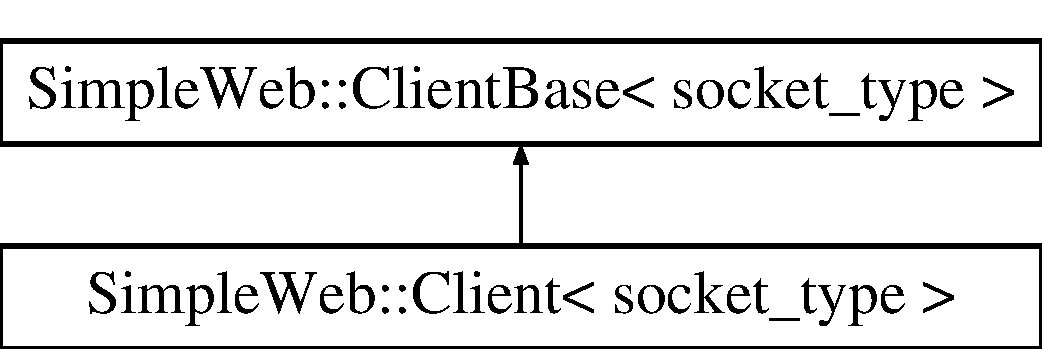
\includegraphics[height=2.000000cm]{a00942}
\end{center}
\end{figure}
\subsection*{Additional Inherited Members}


The documentation for this class was generated from the following file\+:\begin{DoxyCompactItemize}
\item 
client\+\_\+http.\+hpp\end{DoxyCompactItemize}

\hypertarget{a00966}{}\section{Simple\+Web\+:\+:Server$<$ socket\+\_\+type $>$ Class Template Reference}
\label{a00966}\index{Simple\+Web\+::\+Server$<$ socket\+\_\+type $>$@{Simple\+Web\+::\+Server$<$ socket\+\_\+type $>$}}
Inheritance diagram for Simple\+Web\+:\+:Server$<$ socket\+\_\+type $>$\+:\begin{figure}[H]
\begin{center}
\leavevmode
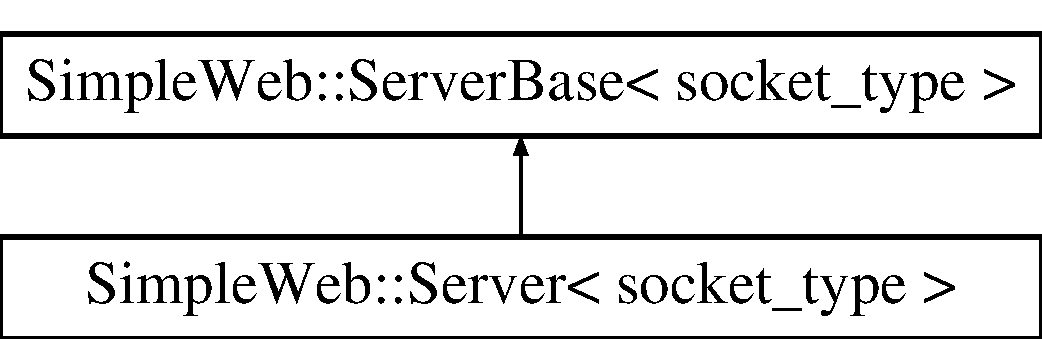
\includegraphics[height=2.000000cm]{a00966}
\end{center}
\end{figure}
\subsection*{Additional Inherited Members}


The documentation for this class was generated from the following file\+:\begin{DoxyCompactItemize}
\item 
server\+\_\+http.\+hpp\end{DoxyCompactItemize}

\hypertarget{a00958}{}\section{Simple\+Web\+:\+:Server$<$ socket\+\_\+type $>$ Class Template Reference}
\label{a00958}\index{Simple\+Web\+::\+Server$<$ socket\+\_\+type $>$@{Simple\+Web\+::\+Server$<$ socket\+\_\+type $>$}}
Inheritance diagram for Simple\+Web\+:\+:Server$<$ socket\+\_\+type $>$\+:\begin{figure}[H]
\begin{center}
\leavevmode
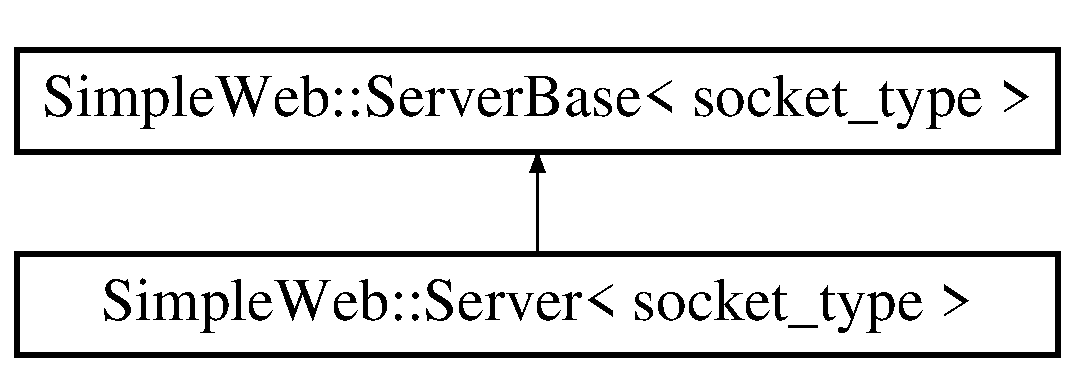
\includegraphics[height=2.000000cm]{a00958}
\end{center}
\end{figure}
\subsection*{Additional Inherited Members}


The documentation for this class was generated from the following file\+:\begin{DoxyCompactItemize}
\item 
server\+\_\+http.\+hpp\end{DoxyCompactItemize}

\hypertarget{a00986}{}\section{Simple\+Web\+:\+:Server\+Base$<$ socket\+\_\+type $>$\+:\+:Config Class Reference}
\label{a00986}\index{Simple\+Web\+::\+Server\+Base$<$ socket\+\_\+type $>$\+::\+Config@{Simple\+Web\+::\+Server\+Base$<$ socket\+\_\+type $>$\+::\+Config}}
\subsection*{Public Attributes}
\begin{DoxyCompactItemize}
\item 
\mbox{\Hypertarget{a00986_aa80030952ff056db08f736d5537bd2c9}\label{a00986_aa80030952ff056db08f736d5537bd2c9}} 
unsigned short \hyperlink{a00986_aa80030952ff056db08f736d5537bd2c9}{port}
\begin{DoxyCompactList}\small\item\em Port number to use. Defaults to 80 for H\+T\+TP and 443 for H\+T\+T\+PS. \end{DoxyCompactList}\item 
\mbox{\Hypertarget{a00986_abfbbfc38bfd2887739676424509dbb45}\label{a00986_abfbbfc38bfd2887739676424509dbb45}} 
size\+\_\+t \hyperlink{a00986_abfbbfc38bfd2887739676424509dbb45}{thread\+\_\+pool\+\_\+size} =1
\begin{DoxyCompactList}\small\item\em Number of threads that the server will use when start() is called. Defaults to 1 thread. \end{DoxyCompactList}\item 
\mbox{\Hypertarget{a00986_aa27e09c83d7e26dff6e72e8d1084d5a0}\label{a00986_aa27e09c83d7e26dff6e72e8d1084d5a0}} 
size\+\_\+t \hyperlink{a00986_aa27e09c83d7e26dff6e72e8d1084d5a0}{timeout\+\_\+request} =5
\begin{DoxyCompactList}\small\item\em Timeout on request handling. Defaults to 5 seconds. \end{DoxyCompactList}\item 
\mbox{\Hypertarget{a00986_ac1f74ff91196c3a72446786b54a77b58}\label{a00986_ac1f74ff91196c3a72446786b54a77b58}} 
size\+\_\+t \hyperlink{a00986_ac1f74ff91196c3a72446786b54a77b58}{timeout\+\_\+content} =300
\begin{DoxyCompactList}\small\item\em Timeout on content handling. Defaults to 300 seconds. \end{DoxyCompactList}\item 
std\+::string \hyperlink{a00986_add7a705aca3533bf0371708b19bb691c}{address}
\item 
\mbox{\Hypertarget{a00986_aab9c347da5390b176d37dac2dfbd9fae}\label{a00986_aab9c347da5390b176d37dac2dfbd9fae}} 
bool \hyperlink{a00986_aab9c347da5390b176d37dac2dfbd9fae}{reuse\+\_\+address} =true
\begin{DoxyCompactList}\small\item\em Set to false to avoid binding the socket to an address that is already in use. Defaults to true. \end{DoxyCompactList}\end{DoxyCompactItemize}
\subsection*{Friends}
\begin{DoxyCompactItemize}
\item 
\mbox{\Hypertarget{a00986_a01d54a7e16ca437c98ec571deca98dfc}\label{a00986_a01d54a7e16ca437c98ec571deca98dfc}} 
class {\bfseries Server\+Base$<$ socket\+\_\+type $>$}
\end{DoxyCompactItemize}


\subsection{Member Data Documentation}
\mbox{\Hypertarget{a00986_add7a705aca3533bf0371708b19bb691c}\label{a00986_add7a705aca3533bf0371708b19bb691c}} 
\index{Simple\+Web\+::\+Server\+Base\+::\+Config@{Simple\+Web\+::\+Server\+Base\+::\+Config}!address@{address}}
\index{address@{address}!Simple\+Web\+::\+Server\+Base\+::\+Config@{Simple\+Web\+::\+Server\+Base\+::\+Config}}
\subsubsection{\texorpdfstring{address}{address}}
{\footnotesize\ttfamily template$<$class socket\+\_\+type$>$ \\
std\+::string \hyperlink{a00970}{Simple\+Web\+::\+Server\+Base}$<$ socket\+\_\+type $>$\+::Config\+::address}

I\+Pv4 address in dotted decimal form or I\+Pv6 address in hexadecimal notation. If empty, the address will be any address. 

The documentation for this class was generated from the following file\+:\begin{DoxyCompactItemize}
\item 
server\+\_\+http.\+hpp\end{DoxyCompactItemize}

\hypertarget{a00990}{}\section{Simple\+Web\+:\+:Server$<$ H\+T\+T\+PS $>$ Class Template Reference}
\label{a00990}\index{Simple\+Web\+::\+Server$<$ H\+T\+T\+P\+S $>$@{Simple\+Web\+::\+Server$<$ H\+T\+T\+P\+S $>$}}
Inheritance diagram for Simple\+Web\+:\+:Server$<$ H\+T\+T\+PS $>$\+:\begin{figure}[H]
\begin{center}
\leavevmode
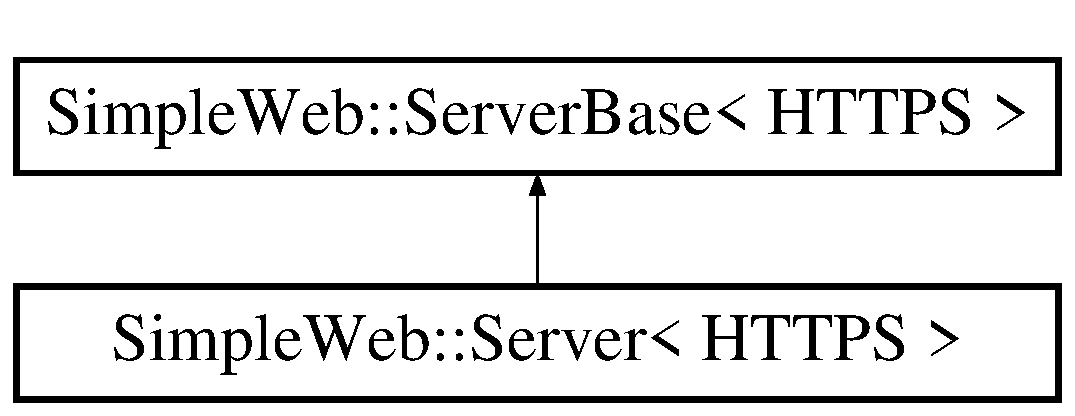
\includegraphics[height=2.000000cm]{a00990}
\end{center}
\end{figure}
\subsection*{Public Member Functions}
\begin{DoxyCompactItemize}
\item 
\mbox{\Hypertarget{a00990_a1a5530e96cd973de3dc987034ca61b54}\label{a00990_a1a5530e96cd973de3dc987034ca61b54}} 
D\+E\+P\+R\+E\+C\+A\+T\+ED {\bfseries Server} (unsigned short port, size\+\_\+t thread\+\_\+pool\+\_\+size, const std\+::string \&cert\+\_\+file, const std\+::string \&private\+\_\+key\+\_\+file, long timeout\+\_\+request=5, long timeout\+\_\+content=300, const std\+::string \&verify\+\_\+file=std\+::string())
\item 
\mbox{\Hypertarget{a00990_a15bb179287dfaa18da16b8877174e8d6}\label{a00990_a15bb179287dfaa18da16b8877174e8d6}} 
{\bfseries Server} (const std\+::string \&cert\+\_\+file, const std\+::string \&private\+\_\+key\+\_\+file, const std\+::string \&verify\+\_\+file=std\+::string())
\item 
\mbox{\Hypertarget{a00990_a6a740b3fdbbbf178f540e27942cc93fc}\label{a00990_a6a740b3fdbbbf178f540e27942cc93fc}} 
void {\bfseries start} ()
\end{DoxyCompactItemize}
\subsection*{Protected Member Functions}
\begin{DoxyCompactItemize}
\item 
\mbox{\Hypertarget{a00990_af722d2884eafafada7073feb7793c422}\label{a00990_af722d2884eafafada7073feb7793c422}} 
void {\bfseries accept} ()
\end{DoxyCompactItemize}
\subsection*{Protected Attributes}
\begin{DoxyCompactItemize}
\item 
\mbox{\Hypertarget{a00990_ade0b1e6f826fd76ba6c6253d352fd93c}\label{a00990_ade0b1e6f826fd76ba6c6253d352fd93c}} 
boost\+::asio\+::ssl\+::context {\bfseries context}
\end{DoxyCompactItemize}
\subsection*{Additional Inherited Members}


The documentation for this class was generated from the following file\+:\begin{DoxyCompactItemize}
\item 
server\+\_\+https.\+hpp\end{DoxyCompactItemize}

\hypertarget{a00962}{}\section{Simple\+Web\+:\+:Client$<$ H\+T\+T\+PS $>$ Class Template Reference}
\label{a00962}\index{Simple\+Web\+::\+Client$<$ H\+T\+T\+P\+S $>$@{Simple\+Web\+::\+Client$<$ H\+T\+T\+P\+S $>$}}
Inheritance diagram for Simple\+Web\+:\+:Client$<$ H\+T\+T\+PS $>$\+:\begin{figure}[H]
\begin{center}
\leavevmode
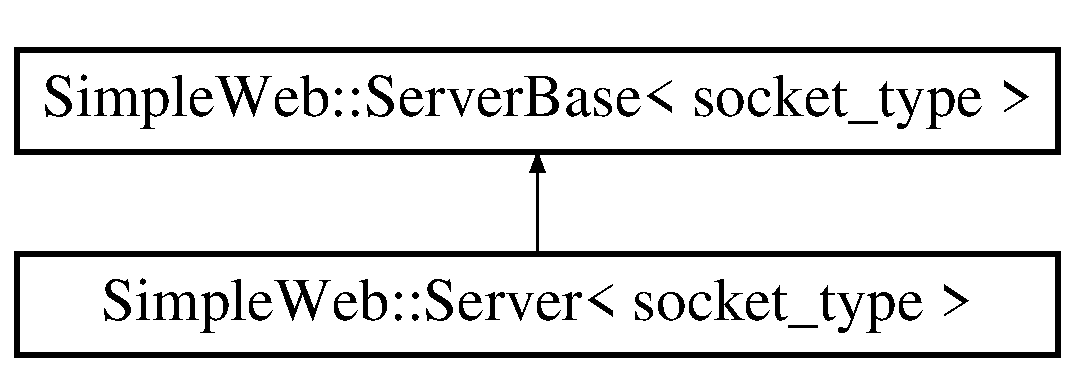
\includegraphics[height=2.000000cm]{a00962}
\end{center}
\end{figure}
\subsection*{Public Member Functions}
\begin{DoxyCompactItemize}
\item 
\mbox{\Hypertarget{a00962_abd87d3dc08c9fed3a60f18c749b8bacd}\label{a00962_abd87d3dc08c9fed3a60f18c749b8bacd}} 
{\bfseries Client} (const std\+::string \&server\+\_\+port\+\_\+path, bool verify\+\_\+certificate=true, const std\+::string \&cert\+\_\+file=std\+::string(), const std\+::string \&private\+\_\+key\+\_\+file=std\+::string(), const std\+::string \&verify\+\_\+file=std\+::string())
\end{DoxyCompactItemize}
\subsection*{Protected Member Functions}
\begin{DoxyCompactItemize}
\item 
\mbox{\Hypertarget{a00962_a833f6fd136e3158b873bee024d6e188c}\label{a00962_a833f6fd136e3158b873bee024d6e188c}} 
void {\bfseries connect} ()
\end{DoxyCompactItemize}
\subsection*{Protected Attributes}
\begin{DoxyCompactItemize}
\item 
\mbox{\Hypertarget{a00962_afe57679cc6153d5d1fe8abc94a8fa58a}\label{a00962_afe57679cc6153d5d1fe8abc94a8fa58a}} 
boost\+::asio\+::ssl\+::context {\bfseries context}
\end{DoxyCompactItemize}
\subsection*{Additional Inherited Members}


The documentation for this class was generated from the following file\+:\begin{DoxyCompactItemize}
\item 
client\+\_\+https.\+hpp\end{DoxyCompactItemize}

\hypertarget{a00914}{}\section{S\+I\+\_\+\+Generic\+Case$<$ S\+I\+\_\+\+C\+H\+AR $>$ Struct Template Reference}
\label{a00914}\index{S\+I\+\_\+\+Generic\+Case$<$ S\+I\+\_\+\+C\+H\+A\+R $>$@{S\+I\+\_\+\+Generic\+Case$<$ S\+I\+\_\+\+C\+H\+A\+R $>$}}


{\ttfamily \#include $<$Simple\+Ini.\+h$>$}

\subsection*{Public Member Functions}
\begin{DoxyCompactItemize}
\item 
\mbox{\Hypertarget{a00914_a786f2c11709bb935c13d9c6ce6a21f7a}\label{a00914_a786f2c11709bb935c13d9c6ce6a21f7a}} 
bool {\bfseries operator()} (const S\+I\+\_\+\+C\+H\+AR $\ast$p\+Left, const S\+I\+\_\+\+C\+H\+AR $\ast$p\+Right) const
\end{DoxyCompactItemize}


\subsection{Detailed Description}
\subsubsection*{template$<$class S\+I\+\_\+\+C\+H\+AR$>$\newline
struct S\+I\+\_\+\+Generic\+Case$<$ S\+I\+\_\+\+C\+H\+A\+R $>$}

Generic case-\/sensitive less than comparison. This class returns numerically ordered A\+S\+C\+II case-\/sensitive text for all possible sizes and types of S\+I\+\_\+\+C\+H\+AR. 

The documentation for this struct was generated from the following file\+:\begin{DoxyCompactItemize}
\item 
Simple\+Ini.\+h\end{DoxyCompactItemize}

\hypertarget{a00918}{}\section{S\+I\+\_\+\+Generic\+No\+Case$<$ S\+I\+\_\+\+C\+H\+AR $>$ Struct Template Reference}
\label{a00918}\index{S\+I\+\_\+\+Generic\+No\+Case$<$ S\+I\+\_\+\+C\+H\+A\+R $>$@{S\+I\+\_\+\+Generic\+No\+Case$<$ S\+I\+\_\+\+C\+H\+A\+R $>$}}


{\ttfamily \#include $<$Simple\+Ini.\+h$>$}

\subsection*{Public Member Functions}
\begin{DoxyCompactItemize}
\item 
\mbox{\Hypertarget{a00918_a5fcbd09e6309590ca9ae6b9981bbac19}\label{a00918_a5fcbd09e6309590ca9ae6b9981bbac19}} 
S\+I\+\_\+\+C\+H\+AR {\bfseries locase} (S\+I\+\_\+\+C\+H\+AR ch) const
\item 
\mbox{\Hypertarget{a00918_aed14252d999472455a769b104afe6c3a}\label{a00918_aed14252d999472455a769b104afe6c3a}} 
bool {\bfseries operator()} (const S\+I\+\_\+\+C\+H\+AR $\ast$p\+Left, const S\+I\+\_\+\+C\+H\+AR $\ast$p\+Right) const
\end{DoxyCompactItemize}


\subsection{Detailed Description}
\subsubsection*{template$<$class S\+I\+\_\+\+C\+H\+AR$>$\newline
struct S\+I\+\_\+\+Generic\+No\+Case$<$ S\+I\+\_\+\+C\+H\+A\+R $>$}

Generic A\+S\+C\+II case-\/insensitive less than comparison. This class returns numerically ordered A\+S\+C\+II case-\/insensitive text for all possible sizes and types of S\+I\+\_\+\+C\+H\+AR. It is not safe for M\+B\+CS text comparison where A\+S\+C\+II A-\/Z characters are used in the encoding of multi-\/byte characters. 

The documentation for this struct was generated from the following file\+:\begin{DoxyCompactItemize}
\item 
Simple\+Ini.\+h\end{DoxyCompactItemize}

\hypertarget{a00906}{}\section{C\+Simple\+Ini\+Templ$<$ S\+I\+\_\+\+C\+H\+AR, S\+I\+\_\+\+S\+T\+R\+L\+E\+SS, S\+I\+\_\+\+C\+O\+N\+V\+E\+R\+T\+ER $>$\+:\+:String\+Writer Class Reference}
\label{a00906}\index{C\+Simple\+Ini\+Templ$<$ S\+I\+\_\+\+C\+H\+A\+R, S\+I\+\_\+\+S\+T\+R\+L\+E\+S\+S, S\+I\+\_\+\+C\+O\+N\+V\+E\+R\+T\+E\+R $>$\+::\+String\+Writer@{C\+Simple\+Ini\+Templ$<$ S\+I\+\_\+\+C\+H\+A\+R, S\+I\+\_\+\+S\+T\+R\+L\+E\+S\+S, S\+I\+\_\+\+C\+O\+N\+V\+E\+R\+T\+E\+R $>$\+::\+String\+Writer}}


{\ttfamily \#include $<$Simple\+Ini.\+h$>$}

Inheritance diagram for C\+Simple\+Ini\+Templ$<$ S\+I\+\_\+\+C\+H\+AR, S\+I\+\_\+\+S\+T\+R\+L\+E\+SS, S\+I\+\_\+\+C\+O\+N\+V\+E\+R\+T\+ER $>$\+:\+:String\+Writer\+:\begin{figure}[H]
\begin{center}
\leavevmode
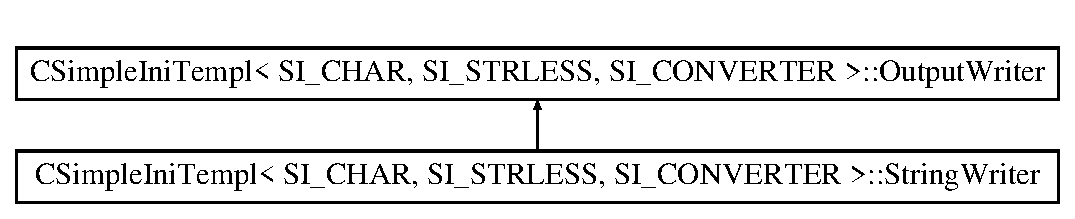
\includegraphics[height=2.000000cm]{a00906}
\end{center}
\end{figure}
\subsection*{Public Member Functions}
\begin{DoxyCompactItemize}
\item 
\mbox{\Hypertarget{a00906_ad50338a07a9b6de7e4a78d0bbc11f67b}\label{a00906_ad50338a07a9b6de7e4a78d0bbc11f67b}} 
{\bfseries String\+Writer} (std\+::string \&a\+\_\+string)
\item 
\mbox{\Hypertarget{a00906_afdfd0dfe71278ea7490a9d4ef6bffadc}\label{a00906_afdfd0dfe71278ea7490a9d4ef6bffadc}} 
void {\bfseries Write} (const char $\ast$a\+\_\+p\+Buf)
\end{DoxyCompactItemize}


\subsection{Detailed Description}
\subsubsection*{template$<$class S\+I\+\_\+\+C\+H\+AR, class S\+I\+\_\+\+S\+T\+R\+L\+E\+SS, class S\+I\+\_\+\+C\+O\+N\+V\+E\+R\+T\+ER$>$\newline
class C\+Simple\+Ini\+Templ$<$ S\+I\+\_\+\+C\+H\+A\+R, S\+I\+\_\+\+S\+T\+R\+L\+E\+S\+S, S\+I\+\_\+\+C\+O\+N\+V\+E\+R\+T\+E\+R $>$\+::\+String\+Writer}

\hyperlink{a00898}{Output\+Writer} class to write the I\+NI data to a string 

The documentation for this class was generated from the following file\+:\begin{DoxyCompactItemize}
\item 
Simple\+Ini.\+h\end{DoxyCompactItemize}

\hypertarget{a00910}{}\section{S\+I\+\_\+\+Generic\+No\+Case$<$ S\+I\+\_\+\+C\+H\+AR $>$ Struct Template Reference}
\label{a00910}\index{S\+I\+\_\+\+Generic\+No\+Case$<$ S\+I\+\_\+\+C\+H\+A\+R $>$@{S\+I\+\_\+\+Generic\+No\+Case$<$ S\+I\+\_\+\+C\+H\+A\+R $>$}}


{\ttfamily \#include $<$Simple\+Ini.\+h$>$}

\subsection*{Public Member Functions}
\begin{DoxyCompactItemize}
\item 
\mbox{\Hypertarget{a00910_a5fcbd09e6309590ca9ae6b9981bbac19}\label{a00910_a5fcbd09e6309590ca9ae6b9981bbac19}} 
S\+I\+\_\+\+C\+H\+AR {\bfseries locase} (S\+I\+\_\+\+C\+H\+AR ch) const
\item 
\mbox{\Hypertarget{a00910_aed14252d999472455a769b104afe6c3a}\label{a00910_aed14252d999472455a769b104afe6c3a}} 
bool {\bfseries operator()} (const S\+I\+\_\+\+C\+H\+AR $\ast$p\+Left, const S\+I\+\_\+\+C\+H\+AR $\ast$p\+Right) const
\end{DoxyCompactItemize}


\subsection{Detailed Description}
\subsubsection*{template$<$class S\+I\+\_\+\+C\+H\+AR$>$\newline
struct S\+I\+\_\+\+Generic\+No\+Case$<$ S\+I\+\_\+\+C\+H\+A\+R $>$}

Generic A\+S\+C\+II case-\/insensitive less than comparison. This class returns numerically ordered A\+S\+C\+II case-\/insensitive text for all possible sizes and types of S\+I\+\_\+\+C\+H\+AR. It is not safe for M\+B\+CS text comparison where A\+S\+C\+II A-\/Z characters are used in the encoding of multi-\/byte characters. 

The documentation for this struct was generated from the following file\+:\begin{DoxyCompactItemize}
\item 
Simple\+Ini.\+h\end{DoxyCompactItemize}

\hypertarget{a00742}{}\section{fire\+:\+:astrophysics\+:\+:Species Struct Reference}
\label{a00742}\index{fire\+::astrophysics\+::\+Species@{fire\+::astrophysics\+::\+Species}}


{\ttfamily \#include $<$Species.\+h$>$}

\subsection*{Public Member Functions}
\begin{DoxyCompactItemize}
\item 
\hyperlink{a00742_ac3c237025b5bcd786519dfbf398f86d3}{Species} (const std\+::vector$<$ std\+::string $>$ \&values)
\end{DoxyCompactItemize}
\subsection*{Public Attributes}
\begin{DoxyCompactItemize}
\item 
const std\+::string \hyperlink{a00742_a4aea10c6b155eaeeb52dedcef2dcf849}{name}
\item 
const int \hyperlink{a00742_a403a85b9ffb625643b0bd5cf2e944376}{mass\+Number}
\item 
const int \hyperlink{a00742_a01796faa4262d2225c4cf3b714afde81}{atomic\+Number}
\item 
const int \hyperlink{a00742_acd295953eb640a1354df0be96e63f1cd}{neutron\+Number}
\item 
double \hyperlink{a00742_aa23c930af303e0c2b09491b18888855b}{mass\+Fraction}
\item 
const double \hyperlink{a00742_a3fd8c01bcbb27c20fb80cf9a9e6e1f66}{mass\+Excess}
\item 
double \hyperlink{a00742_a9a1512c8b681fe0b829b2f91efa8f1a1}{flux}
\end{DoxyCompactItemize}


\subsection{Detailed Description}
This class represents a standard nuclear species within astrophysics such as Helium or Carbon. The mass fraction is the only value on this struct which can be changed.

This class is composed of const-\/qualified members because atomic parameters are immutable. The amount of a species present in a given context varies though. 

\subsection{Constructor \& Destructor Documentation}
\mbox{\Hypertarget{a00742_ac3c237025b5bcd786519dfbf398f86d3}\label{a00742_ac3c237025b5bcd786519dfbf398f86d3}} 
\index{fire\+::astrophysics\+::\+Species@{fire\+::astrophysics\+::\+Species}!Species@{Species}}
\index{Species@{Species}!fire\+::astrophysics\+::\+Species@{fire\+::astrophysics\+::\+Species}}
\subsubsection{\texorpdfstring{Species()}{Species()}}
{\footnotesize\ttfamily fire\+::astrophysics\+::\+Species\+::\+Species (\begin{DoxyParamCaption}\item[{const std\+::vector$<$ std\+::string $>$ \&}]{values }\end{DoxyParamCaption})\hspace{0.3cm}{\ttfamily [inline]}}

The constructor. This class is meant to be initialized from a vector of data created by reading a line from a network file. The vector should have the following entries\+: v\mbox{[}0\mbox{]} -\/ The name v\mbox{[}1\mbox{]} -\/ The mass number v\mbox{[}2\mbox{]} -\/ The atomic number v\mbox{[}3\mbox{]} -\/ The neutron number v\mbox{[}4\mbox{]} -\/ The mass fraction v\mbox{[}5\mbox{]} -\/ The mass excess 
\begin{DoxyParams}{Parameters}
{\em values} & a vector with entries for each of the data members in this class as described above. \\
\hline
\end{DoxyParams}


\subsection{Member Data Documentation}
\mbox{\Hypertarget{a00742_a01796faa4262d2225c4cf3b714afde81}\label{a00742_a01796faa4262d2225c4cf3b714afde81}} 
\index{fire\+::astrophysics\+::\+Species@{fire\+::astrophysics\+::\+Species}!atomic\+Number@{atomic\+Number}}
\index{atomic\+Number@{atomic\+Number}!fire\+::astrophysics\+::\+Species@{fire\+::astrophysics\+::\+Species}}
\subsubsection{\texorpdfstring{atomic\+Number}{atomicNumber}}
{\footnotesize\ttfamily const int fire\+::astrophysics\+::\+Species\+::atomic\+Number}

The total number of protons in the nucleus of this species. Also known as the proton number. Commonly denoted \char`\"{}\+Z.\char`\"{} \mbox{\Hypertarget{a00742_a9a1512c8b681fe0b829b2f91efa8f1a1}\label{a00742_a9a1512c8b681fe0b829b2f91efa8f1a1}} 
\index{fire\+::astrophysics\+::\+Species@{fire\+::astrophysics\+::\+Species}!flux@{flux}}
\index{flux@{flux}!fire\+::astrophysics\+::\+Species@{fire\+::astrophysics\+::\+Species}}
\subsubsection{\texorpdfstring{flux}{flux}}
{\footnotesize\ttfamily double fire\+::astrophysics\+::\+Species\+::flux}

The total flux in the species under current conditions. \mbox{\Hypertarget{a00742_a3fd8c01bcbb27c20fb80cf9a9e6e1f66}\label{a00742_a3fd8c01bcbb27c20fb80cf9a9e6e1f66}} 
\index{fire\+::astrophysics\+::\+Species@{fire\+::astrophysics\+::\+Species}!mass\+Excess@{mass\+Excess}}
\index{mass\+Excess@{mass\+Excess}!fire\+::astrophysics\+::\+Species@{fire\+::astrophysics\+::\+Species}}
\subsubsection{\texorpdfstring{mass\+Excess}{massExcess}}
{\footnotesize\ttfamily const double fire\+::astrophysics\+::\+Species\+::mass\+Excess}

The difference between the actual mass of this species and the mass number. \mbox{\Hypertarget{a00742_aa23c930af303e0c2b09491b18888855b}\label{a00742_aa23c930af303e0c2b09491b18888855b}} 
\index{fire\+::astrophysics\+::\+Species@{fire\+::astrophysics\+::\+Species}!mass\+Fraction@{mass\+Fraction}}
\index{mass\+Fraction@{mass\+Fraction}!fire\+::astrophysics\+::\+Species@{fire\+::astrophysics\+::\+Species}}
\subsubsection{\texorpdfstring{mass\+Fraction}{massFraction}}
{\footnotesize\ttfamily double fire\+::astrophysics\+::\+Species\+::mass\+Fraction}

The fraction of the total mass of the system that is composed of this species. The quantity is normalized to 1.\+0. It is sometimes called the \char`\"{}abundance\char`\"{} as well. \mbox{\Hypertarget{a00742_a403a85b9ffb625643b0bd5cf2e944376}\label{a00742_a403a85b9ffb625643b0bd5cf2e944376}} 
\index{fire\+::astrophysics\+::\+Species@{fire\+::astrophysics\+::\+Species}!mass\+Number@{mass\+Number}}
\index{mass\+Number@{mass\+Number}!fire\+::astrophysics\+::\+Species@{fire\+::astrophysics\+::\+Species}}
\subsubsection{\texorpdfstring{mass\+Number}{massNumber}}
{\footnotesize\ttfamily const int fire\+::astrophysics\+::\+Species\+::mass\+Number}

The total number of nucleons, equal to the sum of the atomic and neutron numbers, in the nucleus of this species. Commonly denoted \char`\"{}\+A.\char`\"{} \mbox{\Hypertarget{a00742_a4aea10c6b155eaeeb52dedcef2dcf849}\label{a00742_a4aea10c6b155eaeeb52dedcef2dcf849}} 
\index{fire\+::astrophysics\+::\+Species@{fire\+::astrophysics\+::\+Species}!name@{name}}
\index{name@{name}!fire\+::astrophysics\+::\+Species@{fire\+::astrophysics\+::\+Species}}
\subsubsection{\texorpdfstring{name}{name}}
{\footnotesize\ttfamily const std\+::string fire\+::astrophysics\+::\+Species\+::name}

The name of this species. \mbox{\Hypertarget{a00742_acd295953eb640a1354df0be96e63f1cd}\label{a00742_acd295953eb640a1354df0be96e63f1cd}} 
\index{fire\+::astrophysics\+::\+Species@{fire\+::astrophysics\+::\+Species}!neutron\+Number@{neutron\+Number}}
\index{neutron\+Number@{neutron\+Number}!fire\+::astrophysics\+::\+Species@{fire\+::astrophysics\+::\+Species}}
\subsubsection{\texorpdfstring{neutron\+Number}{neutronNumber}}
{\footnotesize\ttfamily const int fire\+::astrophysics\+::\+Species\+::neutron\+Number}

The total number of neutrons in the nucleus of this species. Commonly denoted \char`\"{}\+N.\char`\"{} 

The documentation for this struct was generated from the following file\+:\begin{DoxyCompactItemize}
\item 
Species.\+h\end{DoxyCompactItemize}

\hypertarget{a00818}{}\section{fire\+:\+:State$<$ T $>$ Class Template Reference}
\label{a00818}\index{fire\+::\+State$<$ T $>$@{fire\+::\+State$<$ T $>$}}


{\ttfamily \#include $<$State.\+h$>$}

\subsection*{Public Member Functions}
\begin{DoxyCompactItemize}
\item 
\hyperlink{a00818_a697d926ef53bfa150fdabb31db269c21}{State} ()
\item 
\hyperlink{a00818_a40fd4082cd305e2054208a0b9aaa6ad4}{State} (const long \&num\+Elements)
\item 
\hyperlink{a00818_a1882f10811364f7eaa8732514bef43cf}{State} (std\+::shared\+\_\+ptr$<$ T $>$ domain\+State)
\item 
\hyperlink{a00818_adb435ffb356eb26cf62876ede99b9a30}{State} (std\+::shared\+\_\+ptr$<$ T $>$ domain\+State, const long \&num\+Elements)
\item 
void \hyperlink{a00818_adfb16dbbaab3549c09da734605f815a3}{add\+Monitor} (std\+::function$<$ void(\hyperlink{a00818}{State}$<$ T $>$ \&)$>$ monitor)
\item 
T \& \hyperlink{a00818_a71cec682edafbf5c3b09e9d6dc91f12b}{get} () const
\item 
void \hyperlink{a00818_a5d8acc4d5bdd8942de10d34c55680349}{t} (double t)
\item 
const double \& \hyperlink{a00818_a425a0236c4edc506b30196d352118104}{t} () const
\item 
double $\ast$ \hyperlink{a00818_a54507a9e31127580a2c485ce9829934e}{u} () const
\item 
void \hyperlink{a00818_a1b6b91c51fe4d53f268a33c77fecff11}{u} (double $\ast$data)
\item 
double $\ast$ \hyperlink{a00818_a4d20304931607c1cb27358fb3776a620}{dudt} (const double \&\hyperlink{a00818_a5d8acc4d5bdd8942de10d34c55680349}{t}) const
\item 
void \hyperlink{a00818_a22b2d9e2feb153c819e90a4ac7ee8d72}{size} (const long \&num\+Elements)
\item 
int \hyperlink{a00818_a19f1d7b5ce637db79b96f29bd146842a}{size} () const
\item 
{\footnotesize template$<$$>$ }\\double $\ast$ \hyperlink{a00818_a9cc60054f9342b4a84b29937dc45a6d8}{u} () const
\item 
\mbox{\Hypertarget{a00818_a2a3ffc947a9658d7e7173591460d9424}\label{a00818_a2a3ffc947a9658d7e7173591460d9424}} 
{\footnotesize template$<$$>$ }\\void {\bfseries u} (double $\ast$u\+Data)
\item 
\mbox{\Hypertarget{a00818_afa1168dde00e19cee4a7d6d28b4bf9eb}\label{a00818_afa1168dde00e19cee4a7d6d28b4bf9eb}} 
{\footnotesize template$<$$>$ }\\double $\ast$ {\bfseries dudt} (const double \&\hyperlink{a00818_a5d8acc4d5bdd8942de10d34c55680349}{t}) const
\item 
\mbox{\Hypertarget{a00818_ac2313bde7f5d55daee4097232e9ae5ea}\label{a00818_ac2313bde7f5d55daee4097232e9ae5ea}} 
{\footnotesize template$<$$>$ }\\double $\ast$ {\bfseries u} () const
\item 
\mbox{\Hypertarget{a00818_a93837c9543786144b6517a295ed1fec8}\label{a00818_a93837c9543786144b6517a295ed1fec8}} 
{\footnotesize template$<$$>$ }\\double $\ast$ {\bfseries dudt} (const double \&\hyperlink{a00818_a5d8acc4d5bdd8942de10d34c55680349}{t}) const
\item 
\mbox{\Hypertarget{a00818_ac2313bde7f5d55daee4097232e9ae5ea}\label{a00818_ac2313bde7f5d55daee4097232e9ae5ea}} 
{\footnotesize template$<$$>$ }\\double $\ast$ {\bfseries u} () const
\item 
\mbox{\Hypertarget{a00818_a93837c9543786144b6517a295ed1fec8}\label{a00818_a93837c9543786144b6517a295ed1fec8}} 
{\footnotesize template$<$$>$ }\\double $\ast$ {\bfseries dudt} (const double \&\hyperlink{a00818_a5d8acc4d5bdd8942de10d34c55680349}{t}) const
\end{DoxyCompactItemize}
\subsection*{Protected Member Functions}
\begin{DoxyCompactItemize}
\item 
void \hyperlink{a00818_ad271749a2a4f73c11e82ae28141d3b65}{notify\+Monitors} ()
\end{DoxyCompactItemize}
\subsection*{Protected Attributes}
\begin{DoxyCompactItemize}
\item 
std\+::shared\+\_\+ptr$<$ T $>$ \hyperlink{a00818_a9a75139f1d613abc9fb82600757087f6}{state}
\item 
double \hyperlink{a00818_a4985617940993cea772a7fc977c87237}{t\+Val}
\item 
long \hyperlink{a00818_a08f8f4ea745ae855ef730896efabf1ae}{system\+Size}
\item 
std\+::unique\+\_\+ptr$<$ double $>$ \hyperlink{a00818_aae89d6e350df763d503d7da862f1f30a}{u\+Arr}
\item 
std\+::unique\+\_\+ptr$<$ double $>$ \hyperlink{a00818_a9954ba8c1a12555ca1bf67b6a2bf2b3b}{dudt\+Arr}
\item 
std\+::vector$<$ std\+::function$<$ void(\hyperlink{a00818}{State}$<$ T $>$ \&)$>$ $>$ \hyperlink{a00818_ae1571b0a1c82060e525ce6ce2119ae5e}{monitors}
\end{DoxyCompactItemize}


\subsection{Detailed Description}
\subsubsection*{template$<$typename T$>$\newline
class fire\+::\+State$<$ T $>$}

This is a container class for user-\/provided data structures that can be passed to solvers. It is designed such that container operations are handled by default by the template and clients override the \hyperlink{a00818_a54507a9e31127580a2c485ce9829934e}{u()} and \hyperlink{a00818_a4d20304931607c1cb27358fb3776a620}{dudt()} operations to tailor the behavior for the templated type.

Instances should be constructed using the \hyperlink{a00171_abca66b4f2a1543308b663714bd8b4855}{build$<$$>$()} templates as follows\+: 
\begin{DoxyCode}
State<T> myState = build<T>(); \textcolor{comment}{// If T() takes no arguments}
State<T> myState2 = build<T,int>(); \textcolor{comment}{// If T takes one argument}
State<T> myState3 = build<T,int, const double &>(); \textcolor{comment}{// If T takes 2 args}
\textcolor{comment}{//...etc.}
\end{DoxyCode}


The variable t, when discussed below, is meant to represent a free parameter on which u and du depend. It commonly represents time, but might might also represent some other parameter. It is not explicitly called \char`\"{}time\char`\"{} to keep the interface clean of any concepts that might limit the scope of the class to only data that is used in time integrations, when in fact it can be used in the solution of any initial value problem.

The layout of the state is, in effect, a matrix with size n\+\_\+e $\ast$ n\+\_\+t, where n\+\_\+e is the number of unique elements (or unknowns) considered in the system and n\+\_\+t is the number of values of t at which those values are considered. Thus, in the case where a problem has six unknowns (n\+\_\+e = 6) and fifty time steps (t = time and n\+\_\+t = 50), the state class could represent a 6 x 50 matrix with a total of 300 elements. Note that whether or not \char`\"{}the matrix\char`\"{} is stored in column or row major format is not important.

This class is designed to be greedy and narcissistic. In lieu of allowing users to create and store their own instances of T, it creates (add()) those instances and forces users to interact with references retrieved using the getters. Being so greedy makes it possible for this class to efficiently manage memory with lower implementation overhead and no need to rely on clients to correctly initialize data. The original design of this class called for extensive use of smart pointers (using std\+::share), but there are few computational advantages -\/ if any -\/ compared to simple references. This is because simple references do not incur atomic increment and decrement costs when crossing function boundaries, but smart pointers do. In the author\textquotesingle{}s personal experience, the cost of working with smart pointers can be as much as a factor of two in tight loops with function boundaries. References are, by comparison, free in tight loops. Alternatively, passing a reference to the smart pointer is also free, but it is hardly necessary to share a smart pointer at all if the client does not need to participate in the memory lifecycle of the class, and indeed the practice is not recommended (c.\+f. -\/ Sutter\textquotesingle{}s 2014 talk) at all in that case.

Three operations are provided for working with \char`\"{}fundamental state
vectors\char`\"{} as arrays of doubles, but casual users are warned that these operations are for those implementing fast solvers based on this class and, in general, casual users should stick to add() and \hyperlink{a00818_a71cec682edafbf5c3b09e9d6dc91f12b}{get()}.

\hyperlink{a00818}{State} objects can be monitored by registering a functor with the \hyperlink{a00818_adfb16dbbaab3549c09da734605f815a3}{add\+Monitor()} operation. The simplest example is to use a Lambda as follows\+: 
\begin{DoxyCode}
   \textcolor{comment}{// Register an observer to write a message when the state changes.}
state.add([](State<ReactionNetwork> & state) \{
   std::cout << \textcolor{stringliteral}{"Lambda Test "} << state.t() << std::endl;
   \textcolor{keywordflow}{return};
\});
\end{DoxyCode}
 Monitors are only called when \hyperlink{a00818_a1b6b91c51fe4d53f268a33c77fecff11}{u(double $\ast$)} is called. Classes that create explicit specializations of that function should call \hyperlink{a00818_ad271749a2a4f73c11e82ae28141d3b65}{notify\+Monitors()}, a protected notification function, to notify the monitors if they require that functionality. Simply calling the \hyperlink{a00818_ad271749a2a4f73c11e82ae28141d3b65}{notify\+Monitors()} function immediately before return is sufficient.

This class does not yet consider thread safety issues when calling the monitors or updating the state, so be warned.

Common Errors\+: Declaring T instead of T\& -\/ The C++ compiler will not throw an error in the following scenario and will create a copy instead\+: 
\begin{DoxyCode}
T myT1 = state.get(); \textcolor{comment}{// WRONG - Creates a copy of the state!}
T & myT2 = state.get(); \textcolor{comment}{// Correct - Uses the state by reference.}
\textcolor{keyword}{auto} myT3 = state.get(); \textcolor{comment}{// WRONG - Same as the first case.}
\textcolor{keyword}{auto} & myT4 = state.get(); \textcolor{comment}{// Correct - Same as the second case.}
\end{DoxyCode}


Road Map\+:
\begin{DoxyItemize}
\item Right now the auxilliary storage buffers u\+Arr and udt\+Arr are always allocated. It should be possible to enable or disable this.
\item Should this be thread safe?
\item Would be interesting to name monitors. 
\end{DoxyItemize}

\subsection{Constructor \& Destructor Documentation}
\mbox{\Hypertarget{a00818_a697d926ef53bfa150fdabb31db269c21}\label{a00818_a697d926ef53bfa150fdabb31db269c21}} 
\index{fire\+::\+State@{fire\+::\+State}!State@{State}}
\index{State@{State}!fire\+::\+State@{fire\+::\+State}}
\subsubsection{\texorpdfstring{State()}{State()}\hspace{0.1cm}{\footnotesize\ttfamily [1/4]}}
{\footnotesize\ttfamily template$<$typename T$>$ \\
\hyperlink{a00818}{fire\+::\+State}$<$ T $>$\+::\hyperlink{a00818}{State} (\begin{DoxyParamCaption}{ }\end{DoxyParamCaption})\hspace{0.3cm}{\ttfamily [inline]}}

Constructor \mbox{\Hypertarget{a00818_a40fd4082cd305e2054208a0b9aaa6ad4}\label{a00818_a40fd4082cd305e2054208a0b9aaa6ad4}} 
\index{fire\+::\+State@{fire\+::\+State}!State@{State}}
\index{State@{State}!fire\+::\+State@{fire\+::\+State}}
\subsubsection{\texorpdfstring{State()}{State()}\hspace{0.1cm}{\footnotesize\ttfamily [2/4]}}
{\footnotesize\ttfamily template$<$typename T$>$ \\
\hyperlink{a00818}{fire\+::\+State}$<$ T $>$\+::\hyperlink{a00818}{State} (\begin{DoxyParamCaption}\item[{const long \&}]{num\+Elements }\end{DoxyParamCaption})\hspace{0.3cm}{\ttfamily [inline]}}

Alternative constructor that also sets the system size. 
\begin{DoxyParams}{Parameters}
{\em the} & number of unique data elements in the state \\
\hline
\end{DoxyParams}
\mbox{\Hypertarget{a00818_a1882f10811364f7eaa8732514bef43cf}\label{a00818_a1882f10811364f7eaa8732514bef43cf}} 
\index{fire\+::\+State@{fire\+::\+State}!State@{State}}
\index{State@{State}!fire\+::\+State@{fire\+::\+State}}
\subsubsection{\texorpdfstring{State()}{State()}\hspace{0.1cm}{\footnotesize\ttfamily [3/4]}}
{\footnotesize\ttfamily template$<$typename T$>$ \\
\hyperlink{a00818}{fire\+::\+State}$<$ T $>$\+::\hyperlink{a00818}{State} (\begin{DoxyParamCaption}\item[{std\+::shared\+\_\+ptr$<$ T $>$}]{domain\+State }\end{DoxyParamCaption})\hspace{0.3cm}{\ttfamily [inline]}}

An alternative default constructor that will accept a pre-\/configured unique\+\_\+ptr$<$\+T$>$. In general this constructor should not be called directly by clients. It is used by the \hyperlink{a00171_abca66b4f2a1543308b663714bd8b4855}{build$<$$>$()} builder for State$<$\+T$>$ to safely and easily enable two-\/phase construction where the arguments can be passed to T\textquotesingle{}s constructor without requiring State$<$\+T$>$ to know about those arguments.

This is important because requiring State$<$\+T$>$ to know about the arguments of T\textquotesingle{}s constructor would require declaring those arguments in all client classes of State$<$\+T$>$ that used that version of T, which is an undue burden on the user compared to safely enabling two-\/phase construction. \mbox{\Hypertarget{a00818_adb435ffb356eb26cf62876ede99b9a30}\label{a00818_adb435ffb356eb26cf62876ede99b9a30}} 
\index{fire\+::\+State@{fire\+::\+State}!State@{State}}
\index{State@{State}!fire\+::\+State@{fire\+::\+State}}
\subsubsection{\texorpdfstring{State()}{State()}\hspace{0.1cm}{\footnotesize\ttfamily [4/4]}}
{\footnotesize\ttfamily template$<$typename T$>$ \\
\hyperlink{a00818}{fire\+::\+State}$<$ T $>$\+::\hyperlink{a00818}{State} (\begin{DoxyParamCaption}\item[{std\+::shared\+\_\+ptr$<$ T $>$}]{domain\+State,  }\item[{const long \&}]{num\+Elements }\end{DoxyParamCaption})\hspace{0.3cm}{\ttfamily [inline]}}

An alternative constructor that also sets the system size. Analog of \hyperlink{a00818_a40fd4082cd305e2054208a0b9aaa6ad4}{State(const long \&)}. 

\subsection{Member Function Documentation}
\mbox{\Hypertarget{a00818_adfb16dbbaab3549c09da734605f815a3}\label{a00818_adfb16dbbaab3549c09da734605f815a3}} 
\index{fire\+::\+State@{fire\+::\+State}!add\+Monitor@{add\+Monitor}}
\index{add\+Monitor@{add\+Monitor}!fire\+::\+State@{fire\+::\+State}}
\subsubsection{\texorpdfstring{add\+Monitor()}{addMonitor()}}
{\footnotesize\ttfamily template$<$typename T$>$ \\
void \hyperlink{a00818}{fire\+::\+State}$<$ T $>$\+::add\+Monitor (\begin{DoxyParamCaption}\item[{std\+::function$<$ void(\hyperlink{a00818}{State}$<$ T $>$ \&)$>$}]{monitor }\end{DoxyParamCaption})\hspace{0.3cm}{\ttfamily [inline]}}

This operation registers a function with the state that will be called when the state changes. Multiple functions may be registered with the \hyperlink{a00818}{State} and each will be notified when the state is modified. The monitor may be implemented in many ways, but should only take a single State$<$\+T$>$\& as an input an return void.

When the monitoring function is called, it will be passed a reference to the instance of the \hyperlink{a00818}{State} class that changed, not merely to the maintained type. 
\begin{DoxyParams}{Parameters}
{\em monitor} & the functor that should be notified when the state changes. \\
\hline
\end{DoxyParams}
\mbox{\Hypertarget{a00818_a4d20304931607c1cb27358fb3776a620}\label{a00818_a4d20304931607c1cb27358fb3776a620}} 
\index{fire\+::\+State@{fire\+::\+State}!dudt@{dudt}}
\index{dudt@{dudt}!fire\+::\+State@{fire\+::\+State}}
\subsubsection{\texorpdfstring{dudt()}{dudt()}}
{\footnotesize\ttfamily template$<$typename T$>$ \\
double$\ast$ \hyperlink{a00818}{fire\+::\+State}$<$ T $>$\+::dudt (\begin{DoxyParamCaption}\item[{const double \&}]{t }\end{DoxyParamCaption}) const\hspace{0.3cm}{\ttfamily [inline]}}

This function returns a simple array of size \hyperlink{a00818_a22b2d9e2feb153c819e90a4ac7ee8d72}{State.\+size()} which contains the derivatives of the primary \hyperlink{a00818}{State} variables with respect to t. Thus it behaves identically to u(t), but provides derivatives instead.

Note that calling this function with the value t will not reset the stored value of t! So calling \hyperlink{a00818_a5d8acc4d5bdd8942de10d34c55680349}{t()} before and after this function will always return the same value.


\begin{DoxyParams}{Parameters}
{\em t} & the value of the free variable, normally time, at which the derivatives of state should be retrieved \\
\hline
\end{DoxyParams}
\begin{DoxyReturn}{Returns}
dudt\+Values the derivatives at the given value of t 
\end{DoxyReturn}
\mbox{\Hypertarget{a00818_a71cec682edafbf5c3b09e9d6dc91f12b}\label{a00818_a71cec682edafbf5c3b09e9d6dc91f12b}} 
\index{fire\+::\+State@{fire\+::\+State}!get@{get}}
\index{get@{get}!fire\+::\+State@{fire\+::\+State}}
\subsubsection{\texorpdfstring{get()}{get()}}
{\footnotesize\ttfamily template$<$typename T$>$ \\
T\& \hyperlink{a00818}{fire\+::\+State}$<$ T $>$\+::get (\begin{DoxyParamCaption}{ }\end{DoxyParamCaption}) const\hspace{0.3cm}{\ttfamily [inline]}}

This operation returns the state at the most recent value of t. Please note the following nuances related to the use of \char`\"{}auto\+:\char`\"{} 
\begin{DoxyCode}
State<T> \hyperlink{a00818_a9a75139f1d613abc9fb82600757087f6}{state};
T & myT1 = state.get(); \textcolor{comment}{// Work}
\textcolor{keyword}{auto} & myT2 = state.get(); \textcolor{comment}{// Works - myT2 has type T &}
\textcolor{keyword}{auto} myT3 = state.get(); \textcolor{comment}{// Fails - myT3 has type T and is a copy}
\end{DoxyCode}
 \begin{DoxyReturn}{Returns}
state a reference to the state. 
\end{DoxyReturn}
\mbox{\Hypertarget{a00818_ad271749a2a4f73c11e82ae28141d3b65}\label{a00818_ad271749a2a4f73c11e82ae28141d3b65}} 
\index{fire\+::\+State@{fire\+::\+State}!notify\+Monitors@{notify\+Monitors}}
\index{notify\+Monitors@{notify\+Monitors}!fire\+::\+State@{fire\+::\+State}}
\subsubsection{\texorpdfstring{notify\+Monitors()}{notifyMonitors()}}
{\footnotesize\ttfamily template$<$typename T$>$ \\
void \hyperlink{a00818}{fire\+::\+State}$<$ T $>$\+::notify\+Monitors (\begin{DoxyParamCaption}{ }\end{DoxyParamCaption})\hspace{0.3cm}{\ttfamily [inline]}, {\ttfamily [protected]}}

This function notifies the monitors. \mbox{\Hypertarget{a00818_a22b2d9e2feb153c819e90a4ac7ee8d72}\label{a00818_a22b2d9e2feb153c819e90a4ac7ee8d72}} 
\index{fire\+::\+State@{fire\+::\+State}!size@{size}}
\index{size@{size}!fire\+::\+State@{fire\+::\+State}}
\subsubsection{\texorpdfstring{size()}{size()}\hspace{0.1cm}{\footnotesize\ttfamily [1/2]}}
{\footnotesize\ttfamily template$<$typename T$>$ \\
void \hyperlink{a00818}{fire\+::\+State}$<$ T $>$\+::size (\begin{DoxyParamCaption}\item[{const long \&}]{num\+Elements }\end{DoxyParamCaption})\hspace{0.3cm}{\ttfamily [inline]}}

This operation explicitly sets the number of unique data elements in the state. At present this value is constant for all values of t. present in the state. 
\begin{DoxyParams}{Parameters}
{\em int} & the number of unique data elements in the state \\
\hline
\end{DoxyParams}
\mbox{\Hypertarget{a00818_a19f1d7b5ce637db79b96f29bd146842a}\label{a00818_a19f1d7b5ce637db79b96f29bd146842a}} 
\index{fire\+::\+State@{fire\+::\+State}!size@{size}}
\index{size@{size}!fire\+::\+State@{fire\+::\+State}}
\subsubsection{\texorpdfstring{size()}{size()}\hspace{0.1cm}{\footnotesize\ttfamily [2/2]}}
{\footnotesize\ttfamily template$<$typename T$>$ \\
int \hyperlink{a00818}{fire\+::\+State}$<$ T $>$\+::size (\begin{DoxyParamCaption}{ }\end{DoxyParamCaption}) const\hspace{0.3cm}{\ttfamily [inline]}}

This operation returns the number of unique elements in the state. At present this value is constant for all values of t. This is the size of the arrays u and dudt. \begin{DoxyReturn}{Returns}
int the size of the state and the state arrays 
\end{DoxyReturn}
\mbox{\Hypertarget{a00818_a5d8acc4d5bdd8942de10d34c55680349}\label{a00818_a5d8acc4d5bdd8942de10d34c55680349}} 
\index{fire\+::\+State@{fire\+::\+State}!t@{t}}
\index{t@{t}!fire\+::\+State@{fire\+::\+State}}
\subsubsection{\texorpdfstring{t()}{t()}\hspace{0.1cm}{\footnotesize\ttfamily [1/2]}}
{\footnotesize\ttfamily template$<$typename T$>$ \\
void \hyperlink{a00818}{fire\+::\+State}$<$ T $>$\+::t (\begin{DoxyParamCaption}\item[{double}]{t }\end{DoxyParamCaption})\hspace{0.3cm}{\ttfamily [inline]}}

This operation updates the value of t. 
\begin{DoxyParams}{Parameters}
{\em t} & the new value of t \\
\hline
\end{DoxyParams}
\mbox{\Hypertarget{a00818_a425a0236c4edc506b30196d352118104}\label{a00818_a425a0236c4edc506b30196d352118104}} 
\index{fire\+::\+State@{fire\+::\+State}!t@{t}}
\index{t@{t}!fire\+::\+State@{fire\+::\+State}}
\subsubsection{\texorpdfstring{t()}{t()}\hspace{0.1cm}{\footnotesize\ttfamily [2/2]}}
{\footnotesize\ttfamily template$<$typename T$>$ \\
const double\& \hyperlink{a00818}{fire\+::\+State}$<$ T $>$\+::t (\begin{DoxyParamCaption}{ }\end{DoxyParamCaption}) const\hspace{0.3cm}{\ttfamily [inline]}}

This operation retrieves the most recent value of t. \begin{DoxyReturn}{Returns}
the most recent value of t 
\end{DoxyReturn}
\mbox{\Hypertarget{a00818_a54507a9e31127580a2c485ce9829934e}\label{a00818_a54507a9e31127580a2c485ce9829934e}} 
\index{fire\+::\+State@{fire\+::\+State}!u@{u}}
\index{u@{u}!fire\+::\+State@{fire\+::\+State}}
\subsubsection{\texorpdfstring{u()}{u()}\hspace{0.1cm}{\footnotesize\ttfamily [1/3]}}
{\footnotesize\ttfamily template$<$typename T$>$ \\
double$\ast$ \hyperlink{a00818}{fire\+::\+State}$<$ T $>$\+::u (\begin{DoxyParamCaption}{ }\end{DoxyParamCaption}) const\hspace{0.3cm}{\ttfamily [inline]}}

This function returns a simple array of size \hyperlink{a00818_a22b2d9e2feb153c819e90a4ac7ee8d72}{State.\+size()} which contains the values of the fundamental state vector for this type. This vector is normally used by independent solvers looking to solve systems of equations or analysis routines (regression, etc.) in which case it represents the most recent values of the \char`\"{}unknowns\char`\"{} in the (thus the name \char`\"{}u\char`\"{}). So, for example, when solving the heat equation this could include a vector of temperatures at a given t, but it wouldn\textquotesingle{}t, in general, contain the heat transfer coefficients. The distinction is that the temperature is the unknown in the system and coefficients are already well known.

In general, this function should only be used for coupling to Solvers and other systems by developers and most clients should work with their classes retrieved via the \hyperlink{a00818_a71cec682edafbf5c3b09e9d6dc91f12b}{get()} operation.

\begin{DoxyReturn}{Returns}
u\+Values the state 
\end{DoxyReturn}
\mbox{\Hypertarget{a00818_a1b6b91c51fe4d53f268a33c77fecff11}\label{a00818_a1b6b91c51fe4d53f268a33c77fecff11}} 
\index{fire\+::\+State@{fire\+::\+State}!u@{u}}
\index{u@{u}!fire\+::\+State@{fire\+::\+State}}
\subsubsection{\texorpdfstring{u()}{u()}\hspace{0.1cm}{\footnotesize\ttfamily [2/3]}}
{\footnotesize\ttfamily template$<$typename T$>$ \\
void \hyperlink{a00818}{fire\+::\+State}$<$ T $>$\+::u (\begin{DoxyParamCaption}\item[{double $\ast$}]{data }\end{DoxyParamCaption})\hspace{0.3cm}{\ttfamily [inline]}}

This function sets the values of the unknown quantities. It is the inverse of double $\ast$ \hyperlink{a00818_a54507a9e31127580a2c485ce9829934e}{u()} above and is meant to set the values, at the given value of t, for the same fundamental state vector for t\+\_\+n $>$ t\+\_\+(n-\/1). So, for example, this operation could take an input array for t $>$ t\+\_\+(n-\/1) that represents the values of temperature just solved for in a coupled thermomechanics system. However, it would not take diffusion coefficient or other quantities.

If the result of the getter \hyperlink{a00818_a54507a9e31127580a2c485ce9829934e}{State.\+u()}\+:double$\ast$ (see above) is a pointer that is mapped to an array in the stored instance of T, then it is not necessary to call this operation because editing u$\ast$ directly will update the state. However, in cases where it is desirable to either not map directly to the managed data structure or to use \char`\"{}test values\char`\"{} of u, then this function is a handy convenience function. For example, 
\begin{DoxyCode}
\textcolor{keywordtype}{double} * u = state.u()  \textcolor{comment}{// Get the current state}
\textcolor{keywordtype}{double} t = state.t()    \textcolor{comment}{// and t}
\textcolor{keywordtype}{int} size = state.size() \textcolor{comment}{// and size}

\textcolor{comment}{// Make some test updates to u}
\textcolor{keywordtype}{double} * myU = \textcolor{keyword}{new} \textcolor{keywordtype}{double}[\hyperlink{a00818_a19f1d7b5ce637db79b96f29bd146842a}{size}];
\textcolor{keywordflow}{for} (\textcolor{keywordtype}{int} i = 0; i < \hyperlink{a00818_a19f1d7b5ce637db79b96f29bd146842a}{size}; i++) \{
    myU[i] = u[i] + delta();
    ... bunch of other stuff...
\}

\textcolor{comment}{// Submit the new values}
state.u(myU);
\textcolor{keywordtype}{double} * myDudt = state.dudt();

... other stuff ...

delete myU;
\end{DoxyCode}


The default implementation assumes that u is direct pointer to an array in the underlying type T, so implementations may need to override this operation if they do not map directly to the state instance. Furthermore, this operation assumes that the incoming array should be copied instead of referred to directly.


\begin{DoxyParams}{Parameters}
{\em data} & the values of the unknown state variables to be set. The size of this array is expected to be equal to \hyperlink{a00818_a22b2d9e2feb153c819e90a4ac7ee8d72}{State.\+size()}. \\
\hline
\end{DoxyParams}
\mbox{\Hypertarget{a00818_a9cc60054f9342b4a84b29937dc45a6d8}\label{a00818_a9cc60054f9342b4a84b29937dc45a6d8}} 
\index{fire\+::\+State@{fire\+::\+State}!u@{u}}
\index{u@{u}!fire\+::\+State@{fire\+::\+State}}
\subsubsection{\texorpdfstring{u()}{u()}\hspace{0.1cm}{\footnotesize\ttfamily [3/3]}}
{\footnotesize\ttfamily template$<$$>$ \\
double $\ast$ \hyperlink{a00818}{fire\+::\+State}$<$ \hyperlink{a00738}{Reaction\+Network} $>$\+::u (\begin{DoxyParamCaption}{ }\end{DoxyParamCaption}) const}

namespace astrophysics The following operations are explicit instantiations for the \hyperlink{a00818}{State} state class so that Reaction\+Network can be used in the solver. See \hyperlink{a00095_source}{State.\+h} in solvers/ for more information. 

\subsection{Member Data Documentation}
\mbox{\Hypertarget{a00818_a9954ba8c1a12555ca1bf67b6a2bf2b3b}\label{a00818_a9954ba8c1a12555ca1bf67b6a2bf2b3b}} 
\index{fire\+::\+State@{fire\+::\+State}!dudt\+Arr@{dudt\+Arr}}
\index{dudt\+Arr@{dudt\+Arr}!fire\+::\+State@{fire\+::\+State}}
\subsubsection{\texorpdfstring{dudt\+Arr}{dudtArr}}
{\footnotesize\ttfamily template$<$typename T$>$ \\
std\+::unique\+\_\+ptr$<$double$>$ \hyperlink{a00818}{fire\+::\+State}$<$ T $>$\+::dudt\+Arr\hspace{0.3cm}{\ttfamily [protected]}}

This is a utility array that can be used by clients a buffer for holding state derivative values if they cannot be directly mapped to a member on T. \mbox{\Hypertarget{a00818_ae1571b0a1c82060e525ce6ce2119ae5e}\label{a00818_ae1571b0a1c82060e525ce6ce2119ae5e}} 
\index{fire\+::\+State@{fire\+::\+State}!monitors@{monitors}}
\index{monitors@{monitors}!fire\+::\+State@{fire\+::\+State}}
\subsubsection{\texorpdfstring{monitors}{monitors}}
{\footnotesize\ttfamily template$<$typename T$>$ \\
std\+::vector$<$std\+::function$<$void(\hyperlink{a00818}{State}$<$T$>$\&)$>$ $>$ \hyperlink{a00818}{fire\+::\+State}$<$ T $>$\+::monitors\hspace{0.3cm}{\ttfamily [protected]}}

The list of monitors that should be notified when the state changes. \mbox{\Hypertarget{a00818_a9a75139f1d613abc9fb82600757087f6}\label{a00818_a9a75139f1d613abc9fb82600757087f6}} 
\index{fire\+::\+State@{fire\+::\+State}!state@{state}}
\index{state@{state}!fire\+::\+State@{fire\+::\+State}}
\subsubsection{\texorpdfstring{state}{state}}
{\footnotesize\ttfamily template$<$typename T$>$ \\
std\+::shared\+\_\+ptr$<$T$>$ \hyperlink{a00818}{fire\+::\+State}$<$ T $>$\+::state\hspace{0.3cm}{\ttfamily [protected]}}

The managed instance of the \hyperlink{a00818}{State} of type T. \mbox{\Hypertarget{a00818_a08f8f4ea745ae855ef730896efabf1ae}\label{a00818_a08f8f4ea745ae855ef730896efabf1ae}} 
\index{fire\+::\+State@{fire\+::\+State}!system\+Size@{system\+Size}}
\index{system\+Size@{system\+Size}!fire\+::\+State@{fire\+::\+State}}
\subsubsection{\texorpdfstring{system\+Size}{systemSize}}
{\footnotesize\ttfamily template$<$typename T$>$ \\
long \hyperlink{a00818}{fire\+::\+State}$<$ T $>$\+::system\+Size\hspace{0.3cm}{\ttfamily [protected]}}

The system size of the state. \mbox{\Hypertarget{a00818_a4985617940993cea772a7fc977c87237}\label{a00818_a4985617940993cea772a7fc977c87237}} 
\index{fire\+::\+State@{fire\+::\+State}!t\+Val@{t\+Val}}
\index{t\+Val@{t\+Val}!fire\+::\+State@{fire\+::\+State}}
\subsubsection{\texorpdfstring{t\+Val}{tVal}}
{\footnotesize\ttfamily template$<$typename T$>$ \\
double \hyperlink{a00818}{fire\+::\+State}$<$ T $>$\+::t\+Val\hspace{0.3cm}{\ttfamily [protected]}}

The most recent value of t provided by \hyperlink{a00818_a5d8acc4d5bdd8942de10d34c55680349}{State.\+t()}. \mbox{\Hypertarget{a00818_aae89d6e350df763d503d7da862f1f30a}\label{a00818_aae89d6e350df763d503d7da862f1f30a}} 
\index{fire\+::\+State@{fire\+::\+State}!u\+Arr@{u\+Arr}}
\index{u\+Arr@{u\+Arr}!fire\+::\+State@{fire\+::\+State}}
\subsubsection{\texorpdfstring{u\+Arr}{uArr}}
{\footnotesize\ttfamily template$<$typename T$>$ \\
std\+::unique\+\_\+ptr$<$double$>$ \hyperlink{a00818}{fire\+::\+State}$<$ T $>$\+::u\+Arr\hspace{0.3cm}{\ttfamily [protected]}}

This is a utility array that can be used by clients a buffer for holding state values if they cannot be directly mapped to a member on T. 

The documentation for this class was generated from the following file\+:\begin{DoxyCompactItemize}
\item 
State.\+h\end{DoxyCompactItemize}

\hypertarget{a00782}{}\section{fire\+:\+:String\+Caster$<$ T $>$ Struct Template Reference}
\label{a00782}\index{fire\+::\+String\+Caster$<$ T $>$@{fire\+::\+String\+Caster$<$ T $>$}}


{\ttfamily \#include $<$String\+Caster.\+h$>$}

\subsection*{Static Public Member Functions}
\begin{DoxyCompactItemize}
\item 
\mbox{\Hypertarget{a00782_a2f87754c1c9d5cfe64acebbaafddbbae}\label{a00782_a2f87754c1c9d5cfe64acebbaafddbbae}} 
static T {\bfseries cast} (const string \&value)
\end{DoxyCompactItemize}


\subsection{Detailed Description}
\subsubsection*{template$<$typename T$>$\newline
struct fire\+::\+String\+Caster$<$ T $>$}

Default template for casting strings properly. 

The documentation for this struct was generated from the following file\+:\begin{DoxyCompactItemize}
\item 
String\+Caster.\+h\end{DoxyCompactItemize}

\hypertarget{a00798}{}\section{fire\+:\+:String\+Caster$<$ bool $>$ Struct Template Reference}
\label{a00798}\index{fire\+::\+String\+Caster$<$ bool $>$@{fire\+::\+String\+Caster$<$ bool $>$}}


{\ttfamily \#include $<$String\+Caster.\+h$>$}

\subsection*{Static Public Member Functions}
\begin{DoxyCompactItemize}
\item 
\mbox{\Hypertarget{a00798_a852e5b28ba000a44312d3ebcb3703e48}\label{a00798_a852e5b28ba000a44312d3ebcb3703e48}} 
static bool {\bfseries cast} (const string \&value)
\end{DoxyCompactItemize}


\subsection{Detailed Description}
\subsubsection*{template$<$$>$\newline
struct fire\+::\+String\+Caster$<$ bool $>$}

Implementation of \hyperlink{a00782}{String\+Caster} for bools 

The documentation for this struct was generated from the following file\+:\begin{DoxyCompactItemize}
\item 
String\+Caster.\+h\end{DoxyCompactItemize}

\hypertarget{a00786}{}\section{fire\+:\+:Two\+D\+Robin\+Boundary\+Condition Struct Reference}
\label{a00786}\index{fire\+::\+Two\+D\+Robin\+Boundary\+Condition@{fire\+::\+Two\+D\+Robin\+Boundary\+Condition}}


{\ttfamily \#include $<$F\+E\+M\+Types.\+h$>$}

\subsection*{Public Member Functions}
\begin{DoxyCompactItemize}
\item 
\hyperlink{a00786_a94772dc1ff3c599f3f526e72675dac38}{Two\+D\+Robin\+Boundary\+Condition} ()
\item 
\hyperlink{a00786_a691668fb77499b26336866f608cf42b2}{Two\+D\+Robin\+Boundary\+Condition} (const \hyperlink{a00195_a92dafcc05a788e1065a5792b67f0f70e}{Two\+D\+Node} \&first, const \hyperlink{a00195_a92dafcc05a788e1065a5792b67f0f70e}{Two\+D\+Node} \&second, const std\+::function$<$ double(const double \&)$>$ \&\+\_\+sigma, const std\+::function$<$ double(const double \&)$>$ \&\+\_\+h)
\item 
bool \hyperlink{a00786_a3568bb75ca2ecea61b1dbc4c1b8b5b60}{operator==} (const \hyperlink{a00786}{Two\+D\+Robin\+Boundary\+Condition} \&other\+Cond) const
\item 
bool \hyperlink{a00786_adaa602ac0734d5ed6294f015ab4e2c79}{operator!=} (const \hyperlink{a00786}{Two\+D\+Robin\+Boundary\+Condition} \&other\+Cond) const
\end{DoxyCompactItemize}
\subsection*{Public Attributes}
\begin{DoxyCompactItemize}
\item 
\hyperlink{a00195_a92dafcc05a788e1065a5792b67f0f70e}{Two\+D\+Node} \hyperlink{a00786_ad4db2466fecae72b4dc5068a4d04ec4a}{first\+Node}
\item 
\hyperlink{a00195_a92dafcc05a788e1065a5792b67f0f70e}{Two\+D\+Node} \hyperlink{a00786_a5cfaf9f512560ea73616ba18471234bf}{second\+Node}
\item 
std\+::function$<$ double(const double \&)$>$ \hyperlink{a00786_ab32818260358435239f283ee40651fe8}{sigma}
\item 
std\+::function$<$ double(const double \&)$>$ \hyperlink{a00786_a41dadd7aa9c2d03978d7f0b7b673d684}{h}
\end{DoxyCompactItemize}


\subsection{Detailed Description}
This struct represents a two dimensional Robin Boundary condition in which the condition is defined across an edge between two nodes. The Robin condition is defined as \[ k(s)\frac{\partial u}{\partial n} + \sigma(s) u = h(s) \mbox{ on } C_{2} \] All members of this struct must be initialized on construction. The idea is that the references should not need to change during execution because the boundaries do not change. 

\subsection{Constructor \& Destructor Documentation}
\mbox{\Hypertarget{a00786_a94772dc1ff3c599f3f526e72675dac38}\label{a00786_a94772dc1ff3c599f3f526e72675dac38}} 
\index{fire\+::\+Two\+D\+Robin\+Boundary\+Condition@{fire\+::\+Two\+D\+Robin\+Boundary\+Condition}!Two\+D\+Robin\+Boundary\+Condition@{Two\+D\+Robin\+Boundary\+Condition}}
\index{Two\+D\+Robin\+Boundary\+Condition@{Two\+D\+Robin\+Boundary\+Condition}!fire\+::\+Two\+D\+Robin\+Boundary\+Condition@{fire\+::\+Two\+D\+Robin\+Boundary\+Condition}}
\subsubsection{\texorpdfstring{Two\+D\+Robin\+Boundary\+Condition()}{TwoDRobinBoundaryCondition()}\hspace{0.1cm}{\footnotesize\ttfamily [1/2]}}
{\footnotesize\ttfamily fire\+::\+Two\+D\+Robin\+Boundary\+Condition\+::\+Two\+D\+Robin\+Boundary\+Condition (\begin{DoxyParamCaption}{ }\end{DoxyParamCaption})\hspace{0.3cm}{\ttfamily [inline]}}

The default constructor \mbox{\Hypertarget{a00786_a691668fb77499b26336866f608cf42b2}\label{a00786_a691668fb77499b26336866f608cf42b2}} 
\index{fire\+::\+Two\+D\+Robin\+Boundary\+Condition@{fire\+::\+Two\+D\+Robin\+Boundary\+Condition}!Two\+D\+Robin\+Boundary\+Condition@{Two\+D\+Robin\+Boundary\+Condition}}
\index{Two\+D\+Robin\+Boundary\+Condition@{Two\+D\+Robin\+Boundary\+Condition}!fire\+::\+Two\+D\+Robin\+Boundary\+Condition@{fire\+::\+Two\+D\+Robin\+Boundary\+Condition}}
\subsubsection{\texorpdfstring{Two\+D\+Robin\+Boundary\+Condition()}{TwoDRobinBoundaryCondition()}\hspace{0.1cm}{\footnotesize\ttfamily [2/2]}}
{\footnotesize\ttfamily fire\+::\+Two\+D\+Robin\+Boundary\+Condition\+::\+Two\+D\+Robin\+Boundary\+Condition (\begin{DoxyParamCaption}\item[{const \hyperlink{a00195_a92dafcc05a788e1065a5792b67f0f70e}{Two\+D\+Node} \&}]{first,  }\item[{const \hyperlink{a00195_a92dafcc05a788e1065a5792b67f0f70e}{Two\+D\+Node} \&}]{second,  }\item[{const std\+::function$<$ double(const double \&)$>$ \&}]{\+\_\+sigma,  }\item[{const std\+::function$<$ double(const double \&)$>$ \&}]{\+\_\+h }\end{DoxyParamCaption})\hspace{0.3cm}{\ttfamily [inline]}}

Constructor 
\begin{DoxyParams}{Parameters}
{\em first} & the node that should be used as the first node on the path \\
\hline
{\em second} & the node that should be used as the second or terminal node on the path \\
\hline
{\em \+\_\+sigma} & the sigma function \\
\hline
{\em \+\_\+h} & the h function on the right-\/hand side of the condition \\
\hline
\end{DoxyParams}


\subsection{Member Function Documentation}
\mbox{\Hypertarget{a00786_adaa602ac0734d5ed6294f015ab4e2c79}\label{a00786_adaa602ac0734d5ed6294f015ab4e2c79}} 
\index{fire\+::\+Two\+D\+Robin\+Boundary\+Condition@{fire\+::\+Two\+D\+Robin\+Boundary\+Condition}!operator"!=@{operator"!=}}
\index{operator"!=@{operator"!=}!fire\+::\+Two\+D\+Robin\+Boundary\+Condition@{fire\+::\+Two\+D\+Robin\+Boundary\+Condition}}
\subsubsection{\texorpdfstring{operator"!=()}{operator!=()}}
{\footnotesize\ttfamily bool fire\+::\+Two\+D\+Robin\+Boundary\+Condition\+::operator!= (\begin{DoxyParamCaption}\item[{const \hyperlink{a00786}{Two\+D\+Robin\+Boundary\+Condition} \&}]{other\+Cond }\end{DoxyParamCaption}) const\hspace{0.3cm}{\ttfamily [inline]}}

The inequality operator override to invert ==. \mbox{\Hypertarget{a00786_a3568bb75ca2ecea61b1dbc4c1b8b5b60}\label{a00786_a3568bb75ca2ecea61b1dbc4c1b8b5b60}} 
\index{fire\+::\+Two\+D\+Robin\+Boundary\+Condition@{fire\+::\+Two\+D\+Robin\+Boundary\+Condition}!operator==@{operator==}}
\index{operator==@{operator==}!fire\+::\+Two\+D\+Robin\+Boundary\+Condition@{fire\+::\+Two\+D\+Robin\+Boundary\+Condition}}
\subsubsection{\texorpdfstring{operator==()}{operator==()}}
{\footnotesize\ttfamily bool fire\+::\+Two\+D\+Robin\+Boundary\+Condition\+::operator== (\begin{DoxyParamCaption}\item[{const \hyperlink{a00786}{Two\+D\+Robin\+Boundary\+Condition} \&}]{other\+Cond }\end{DoxyParamCaption}) const\hspace{0.3cm}{\ttfamily [inline]}}

This is an operator override to compare two dimensional Robin conditions. Note that this operation implements equality checks for the functions by generating pointer targets for the functions and checking target types. This may or may not be the best way to check for equality of these functions, depending on your application. 
\begin{DoxyParams}{Parameters}
{\em other\+Cond} & the other condition \\
\hline
\end{DoxyParams}
\begin{DoxyReturn}{Returns}
true if the conditions are equal, false otherwise. 
\end{DoxyReturn}


\subsection{Member Data Documentation}
\mbox{\Hypertarget{a00786_ad4db2466fecae72b4dc5068a4d04ec4a}\label{a00786_ad4db2466fecae72b4dc5068a4d04ec4a}} 
\index{fire\+::\+Two\+D\+Robin\+Boundary\+Condition@{fire\+::\+Two\+D\+Robin\+Boundary\+Condition}!first\+Node@{first\+Node}}
\index{first\+Node@{first\+Node}!fire\+::\+Two\+D\+Robin\+Boundary\+Condition@{fire\+::\+Two\+D\+Robin\+Boundary\+Condition}}
\subsubsection{\texorpdfstring{first\+Node}{firstNode}}
{\footnotesize\ttfamily \hyperlink{a00195_a92dafcc05a788e1065a5792b67f0f70e}{Two\+D\+Node} fire\+::\+Two\+D\+Robin\+Boundary\+Condition\+::first\+Node}

The first node where the edge starts \mbox{\Hypertarget{a00786_a41dadd7aa9c2d03978d7f0b7b673d684}\label{a00786_a41dadd7aa9c2d03978d7f0b7b673d684}} 
\index{fire\+::\+Two\+D\+Robin\+Boundary\+Condition@{fire\+::\+Two\+D\+Robin\+Boundary\+Condition}!h@{h}}
\index{h@{h}!fire\+::\+Two\+D\+Robin\+Boundary\+Condition@{fire\+::\+Two\+D\+Robin\+Boundary\+Condition}}
\subsubsection{\texorpdfstring{h}{h}}
{\footnotesize\ttfamily std\+::function$<$double(const double \&)$>$ fire\+::\+Two\+D\+Robin\+Boundary\+Condition\+::h}

As defined in the definition of the condition. 
\begin{DoxyParams}{Parameters}
{\em s} & The distance along the side length \\
\hline
\end{DoxyParams}
\mbox{\Hypertarget{a00786_a5cfaf9f512560ea73616ba18471234bf}\label{a00786_a5cfaf9f512560ea73616ba18471234bf}} 
\index{fire\+::\+Two\+D\+Robin\+Boundary\+Condition@{fire\+::\+Two\+D\+Robin\+Boundary\+Condition}!second\+Node@{second\+Node}}
\index{second\+Node@{second\+Node}!fire\+::\+Two\+D\+Robin\+Boundary\+Condition@{fire\+::\+Two\+D\+Robin\+Boundary\+Condition}}
\subsubsection{\texorpdfstring{second\+Node}{secondNode}}
{\footnotesize\ttfamily \hyperlink{a00195_a92dafcc05a788e1065a5792b67f0f70e}{Two\+D\+Node} fire\+::\+Two\+D\+Robin\+Boundary\+Condition\+::second\+Node}

The second node where the edge terminates \mbox{\Hypertarget{a00786_ab32818260358435239f283ee40651fe8}\label{a00786_ab32818260358435239f283ee40651fe8}} 
\index{fire\+::\+Two\+D\+Robin\+Boundary\+Condition@{fire\+::\+Two\+D\+Robin\+Boundary\+Condition}!sigma@{sigma}}
\index{sigma@{sigma}!fire\+::\+Two\+D\+Robin\+Boundary\+Condition@{fire\+::\+Two\+D\+Robin\+Boundary\+Condition}}
\subsubsection{\texorpdfstring{sigma}{sigma}}
{\footnotesize\ttfamily std\+::function$<$double(const double \&)$>$ fire\+::\+Two\+D\+Robin\+Boundary\+Condition\+::sigma}

As defined in the definition of the condition. 
\begin{DoxyParams}{Parameters}
{\em s} & The distance along the side length \\
\hline
\end{DoxyParams}


The documentation for this struct was generated from the following file\+:\begin{DoxyCompactItemize}
\item 
F\+E\+M\+Types.\+h\end{DoxyCompactItemize}

\hypertarget{a00790}{}\section{fire\+:\+:String\+Caster$<$ float $>$ Struct Template Reference}
\label{a00790}\index{fire\+::\+String\+Caster$<$ float $>$@{fire\+::\+String\+Caster$<$ float $>$}}


{\ttfamily \#include $<$String\+Caster.\+h$>$}

\subsection*{Static Public Member Functions}
\begin{DoxyCompactItemize}
\item 
\mbox{\Hypertarget{a00790_a3dbc17ad2b6b2185fea43993871f24f7}\label{a00790_a3dbc17ad2b6b2185fea43993871f24f7}} 
static double {\bfseries cast} (const string \&value)
\end{DoxyCompactItemize}


\subsection{Detailed Description}
\subsubsection*{template$<$$>$\newline
struct fire\+::\+String\+Caster$<$ float $>$}

Implementation of \hyperlink{a00782}{String\+Caster} for floats 

The documentation for this struct was generated from the following file\+:\begin{DoxyCompactItemize}
\item 
String\+Caster.\+h\end{DoxyCompactItemize}

\hypertarget{a00794}{}\section{fire\+:\+:String\+Caster$<$ int $>$ Struct Template Reference}
\label{a00794}\index{fire\+::\+String\+Caster$<$ int $>$@{fire\+::\+String\+Caster$<$ int $>$}}


{\ttfamily \#include $<$String\+Caster.\+h$>$}

\subsection*{Static Public Member Functions}
\begin{DoxyCompactItemize}
\item 
\mbox{\Hypertarget{a00794_a62373040bdd4acb9e2c890d83829e22f}\label{a00794_a62373040bdd4acb9e2c890d83829e22f}} 
static double {\bfseries cast} (const string \&value)
\end{DoxyCompactItemize}


\subsection{Detailed Description}
\subsubsection*{template$<$$>$\newline
struct fire\+::\+String\+Caster$<$ int $>$}

Implementation of \hyperlink{a00782}{String\+Caster} for ints 

The documentation for this struct was generated from the following file\+:\begin{DoxyCompactItemize}
\item 
String\+Caster.\+h\end{DoxyCompactItemize}

\hypertarget{a00898}{}\section{C\+Simple\+Ini\+Templ$<$ S\+I\+\_\+\+C\+H\+AR, S\+I\+\_\+\+S\+T\+R\+L\+E\+SS, S\+I\+\_\+\+C\+O\+N\+V\+E\+R\+T\+ER $>$\+:\+:String\+Writer Class Reference}
\label{a00898}\index{C\+Simple\+Ini\+Templ$<$ S\+I\+\_\+\+C\+H\+A\+R, S\+I\+\_\+\+S\+T\+R\+L\+E\+S\+S, S\+I\+\_\+\+C\+O\+N\+V\+E\+R\+T\+E\+R $>$\+::\+String\+Writer@{C\+Simple\+Ini\+Templ$<$ S\+I\+\_\+\+C\+H\+A\+R, S\+I\+\_\+\+S\+T\+R\+L\+E\+S\+S, S\+I\+\_\+\+C\+O\+N\+V\+E\+R\+T\+E\+R $>$\+::\+String\+Writer}}


{\ttfamily \#include $<$Simple\+Ini.\+h$>$}

Inheritance diagram for C\+Simple\+Ini\+Templ$<$ S\+I\+\_\+\+C\+H\+AR, S\+I\+\_\+\+S\+T\+R\+L\+E\+SS, S\+I\+\_\+\+C\+O\+N\+V\+E\+R\+T\+ER $>$\+:\+:String\+Writer\+:\begin{figure}[H]
\begin{center}
\leavevmode
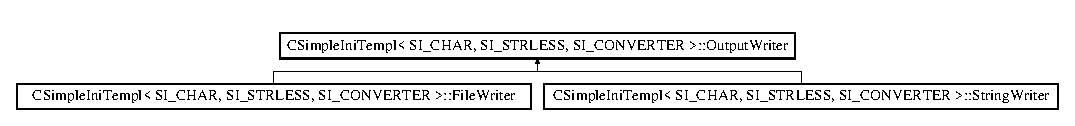
\includegraphics[height=2.000000cm]{a00898}
\end{center}
\end{figure}
\subsection*{Public Member Functions}
\begin{DoxyCompactItemize}
\item 
\mbox{\Hypertarget{a00898_ad50338a07a9b6de7e4a78d0bbc11f67b}\label{a00898_ad50338a07a9b6de7e4a78d0bbc11f67b}} 
{\bfseries String\+Writer} (std\+::string \&a\+\_\+string)
\item 
\mbox{\Hypertarget{a00898_afdfd0dfe71278ea7490a9d4ef6bffadc}\label{a00898_afdfd0dfe71278ea7490a9d4ef6bffadc}} 
void {\bfseries Write} (const char $\ast$a\+\_\+p\+Buf)
\end{DoxyCompactItemize}


\subsection{Detailed Description}
\subsubsection*{template$<$class S\+I\+\_\+\+C\+H\+AR, class S\+I\+\_\+\+S\+T\+R\+L\+E\+SS, class S\+I\+\_\+\+C\+O\+N\+V\+E\+R\+T\+ER$>$\newline
class C\+Simple\+Ini\+Templ$<$ S\+I\+\_\+\+C\+H\+A\+R, S\+I\+\_\+\+S\+T\+R\+L\+E\+S\+S, S\+I\+\_\+\+C\+O\+N\+V\+E\+R\+T\+E\+R $>$\+::\+String\+Writer}

\hyperlink{a00890}{Output\+Writer} class to write the I\+NI data to a string 

The documentation for this class was generated from the following file\+:\begin{DoxyCompactItemize}
\item 
Simple\+Ini.\+h\end{DoxyCompactItemize}

\hypertarget{a00754}{}\section{fire\+:\+:System$<$ T $>$ Class Template Reference}
\label{a00754}\index{fire\+::\+System$<$ T $>$@{fire\+::\+System$<$ T $>$}}


{\ttfamily \#include $<$System.\+h$>$}

\subsection*{Public Member Functions}
\begin{DoxyCompactItemize}
\item 
void \hyperlink{a00754_a2c252b0ec85877bcfcbae60dff04dfaa}{set\+Size} (const long \&n, const short \&d)
\item 
void \hyperlink{a00754_aa9e25fbc00a50d54fb90ac1fdcd911e4}{set\+State} (T $\ast$system\+State)
\end{DoxyCompactItemize}
\subsection*{Protected Attributes}
\begin{DoxyCompactItemize}
\item 
long \hyperlink{a00754_a89101170e69beff93e11c795aa6bb481}{num\+Eqs}
\item 
short \hyperlink{a00754_a041623ed0162d4cad4309c9be3e7df9d}{n\+Dim}
\item 
T $\ast$ \hyperlink{a00754_ac59dffce1577673d04cd222c0f769c11}{state}
\end{DoxyCompactItemize}


\subsection{Detailed Description}
\subsubsection*{template$<$class T$>$\newline
class fire\+::\+System$<$ T $>$}

This class represents a system of equations in Fire, where a system of equations is a collection of equations with the same unknowns.

The system of equations is represented by a collection of operators that operate on a problem state provided by the user. The state defines all of the system\textquotesingle{}s unknown quantities. However, since the type of the state is generic, the system does not explicitly known the identity of those unknowns. The user-\/defined state class is expected to provide the unknowns contiguously when queried.

The system of equations can be integrated by calling the integrate() operation. The system will be solved using a default integrator if a user-\/ defined integrator is not provided. 

\subsection{Member Function Documentation}
\mbox{\Hypertarget{a00754_a2c252b0ec85877bcfcbae60dff04dfaa}\label{a00754_a2c252b0ec85877bcfcbae60dff04dfaa}} 
\index{fire\+::\+System@{fire\+::\+System}!set\+Size@{set\+Size}}
\index{set\+Size@{set\+Size}!fire\+::\+System@{fire\+::\+System}}
\subsubsection{\texorpdfstring{set\+Size()}{setSize()}}
{\footnotesize\ttfamily template$<$class T $>$ \\
void \hyperlink{a00754}{fire\+::\+System}$<$ T $>$\+::set\+Size (\begin{DoxyParamCaption}\item[{const long \&}]{n,  }\item[{const short \&}]{d }\end{DoxyParamCaption})\hspace{0.3cm}{\ttfamily [inline]}}

This operation sets the size of the system of equations by defining the total number of equations and the number of dimensions. 
\begin{DoxyParams}{Parameters}
{\em n} & The total number of equations in the system. \\
\hline
{\em d} & The total number of physical dimensions of the system, not including time. 1 for 1D, 2 for 2D, 3 for 3D. \\
\hline
\end{DoxyParams}
\mbox{\Hypertarget{a00754_aa9e25fbc00a50d54fb90ac1fdcd911e4}\label{a00754_aa9e25fbc00a50d54fb90ac1fdcd911e4}} 
\index{fire\+::\+System@{fire\+::\+System}!set\+State@{set\+State}}
\index{set\+State@{set\+State}!fire\+::\+System@{fire\+::\+System}}
\subsubsection{\texorpdfstring{set\+State()}{setState()}}
{\footnotesize\ttfamily template$<$class T $>$ \\
void \hyperlink{a00754}{fire\+::\+System}$<$ T $>$\+::set\+State (\begin{DoxyParamCaption}\item[{T $\ast$}]{system\+State }\end{DoxyParamCaption})\hspace{0.3cm}{\ttfamily [inline]}}

This operation specifies the state of the system of equations.

The state is provided using a raw pointer because the system of equations does not participate in the state\textquotesingle{}s memory lifecycle. This class explicitly guarantees that it will never deallocate the state data! Classes utilized by this class, such as integrators, may overwrite or manipulate the state data in ways described in their A\+PI docs, including attempting to deallocate it (frowned upon). Clients should generally expect that the state variables provided by the state type T will be modified and that in some instances those modifications may be done in place. 

\subsection{Member Data Documentation}
\mbox{\Hypertarget{a00754_a041623ed0162d4cad4309c9be3e7df9d}\label{a00754_a041623ed0162d4cad4309c9be3e7df9d}} 
\index{fire\+::\+System@{fire\+::\+System}!n\+Dim@{n\+Dim}}
\index{n\+Dim@{n\+Dim}!fire\+::\+System@{fire\+::\+System}}
\subsubsection{\texorpdfstring{n\+Dim}{nDim}}
{\footnotesize\ttfamily template$<$class T $>$ \\
short \hyperlink{a00754}{fire\+::\+System}$<$ T $>$\+::n\+Dim\hspace{0.3cm}{\ttfamily [protected]}}

The total number of physical dimensions of the system, not including time. \mbox{\Hypertarget{a00754_a89101170e69beff93e11c795aa6bb481}\label{a00754_a89101170e69beff93e11c795aa6bb481}} 
\index{fire\+::\+System@{fire\+::\+System}!num\+Eqs@{num\+Eqs}}
\index{num\+Eqs@{num\+Eqs}!fire\+::\+System@{fire\+::\+System}}
\subsubsection{\texorpdfstring{num\+Eqs}{numEqs}}
{\footnotesize\ttfamily template$<$class T $>$ \\
long \hyperlink{a00754}{fire\+::\+System}$<$ T $>$\+::num\+Eqs\hspace{0.3cm}{\ttfamily [protected]}}

The total number of equations in the system. \mbox{\Hypertarget{a00754_ac59dffce1577673d04cd222c0f769c11}\label{a00754_ac59dffce1577673d04cd222c0f769c11}} 
\index{fire\+::\+System@{fire\+::\+System}!state@{state}}
\index{state@{state}!fire\+::\+System@{fire\+::\+System}}
\subsubsection{\texorpdfstring{state}{state}}
{\footnotesize\ttfamily template$<$class T $>$ \\
T$\ast$ \hyperlink{a00754}{fire\+::\+System}$<$ T $>$\+::state\hspace{0.3cm}{\ttfamily [protected]}}

The state of the system, including unknowns, materials information, etc. 

The documentation for this class was generated from the following file\+:\begin{DoxyCompactItemize}
\item 
System.\+h\end{DoxyCompactItemize}

\hypertarget{a00838}{}\section{fire\+:\+:Tensor$<$ Rank, Derived\+Tensor\+Backend\+Builder, Scalar $>$ Class Template Reference}
\label{a00838}\index{fire\+::\+Tensor$<$ Rank, Derived\+Tensor\+Backend\+Builder, Scalar $>$@{fire\+::\+Tensor$<$ Rank, Derived\+Tensor\+Backend\+Builder, Scalar $>$}}


{\ttfamily \#include $<$Tensor.\+hpp$>$}

\subsection*{Public Member Functions}
\begin{DoxyCompactItemize}
\item 
\hyperlink{a00838_a483bba67036bbf284bf916b3ba08973d}{Tensor} (\hyperlink{a00171_a1bf491fd1c876e2808648b2fd291e3dd}{Tensor\+Reference}$<$ Scalar $>$ \&reference)
\item 
{\footnotesize template$<$typename ... Dimension$>$ }\\\hyperlink{a00838_a21e6407bfc23f1dd7fae405d5a9e5575}{Tensor} (int first\+Dim, Dimension ... other\+Dims)
\item 
\hyperlink{a00838_a4b2b898dd5d6c9dec53d0fa1bf0c6591}{Tensor} (std\+::array$<$ int, Rank $>$ dimensions)
\item 
{\footnotesize template$<$typename ... Indices$>$ }\\Scalar \& \hyperlink{a00838_a07cc44df958ab73a79d15c6d96fa5544}{operator()} (Indices ... indices) const
\item 
\hyperlink{a00838_ac86105ceb5e209854b2554a755024bd4}{This\+Tensor\+Type} \hyperlink{a00838_a20377472ae56dcaa2c0f67feb13900e7}{operator+} (\hyperlink{a00838_ac86105ceb5e209854b2554a755024bd4}{This\+Tensor\+Type} \&other)
\item 
bool \hyperlink{a00838_a5f24a2528292de76b6c52e2cc99acf9c}{operator==} (\hyperlink{a00838_ac86105ceb5e209854b2554a755024bd4}{This\+Tensor\+Type} \&other)
\item 
bool \hyperlink{a00838_a53ac3eadb4a5047c56e749b7e7c4d53d}{operator!=} (\hyperlink{a00838_ac86105ceb5e209854b2554a755024bd4}{This\+Tensor\+Type} \&other)
\item 
{\footnotesize template$<$typename Other\+Derived , typename Contraction\+Dims $>$ }\\\hyperlink{a00838}{Tensor}$<$ Derived\+Tensor\+Backend\+::get\+Rank()+Other\+Derived\+::get\+Rank() -\/ 2 $\ast$\hyperlink{a00854}{array\+\_\+size}$<$ Contraction\+Dims $>$\+::value, Derived\+Tensor\+Backend\+Builder, Scalar $>$ \hyperlink{a00838_abf5a45aa771a93365950eb5093a8304c}{contract} (Other\+Derived \&other, Contraction\+Dims \&indices)
\item 
{\footnotesize template$<$typename Other\+Derived $>$ }\\\hyperlink{a00838}{Tensor}$<$ Derived\+Tensor\+Backend\+::get\+Rank()+Other\+Derived\+::get\+Rank(), Derived\+Tensor\+Backend\+Builder, Scalar $>$ \hyperlink{a00838_a67952b93c6812069d521522bf9b3b887}{operator$\ast$} (Other\+Derived \&other)
\item 
void \hyperlink{a00838_acbe638bc3fbd75bf67f4a25467f95594}{set\+Random} ()
\item 
int \hyperlink{a00838_aa2f9181f6fab4a276ef2c9b1637af912}{dimension} (int index)
\item 
\hyperlink{a00171_a1bf491fd1c876e2808648b2fd291e3dd}{Tensor\+Reference}$<$ Scalar $>$ \hyperlink{a00838_a54f4e46000baf9132b6953abc03dd7b7}{create\+Reference} ()
\item 
void \hyperlink{a00838_a1ba79b5076cb6483929fc33bd06d1485}{set\+Values} (const typename \hyperlink{a00862}{fire\+::\+Initializer}$<$ \hyperlink{a00838_ac86105ceb5e209854b2554a755024bd4}{This\+Tensor\+Type}, Scalar, Rank $>$\+::Init\+List \&vals)
\item 
\hyperlink{a00838_ac86105ceb5e209854b2554a755024bd4}{This\+Tensor\+Type} \hyperlink{a00838_a6de8950823ff713b7226e332b02f15f8}{operator$\ast$} (Scalar val)
\item 
void \hyperlink{a00838_a98fae67b5aa6dfdc9ccc429e72a92d64}{print} (std\+::ostream \&output\+Stream)
\item 
const int \hyperlink{a00838_a595b6b9b26549cc2d866e1780fb7a91f}{size} ()
\item 
{\footnotesize template$<$typename Dim\+Array $>$ }\\\hyperlink{a00838}{Tensor}$<$ \hyperlink{a00854}{array\+\_\+size}$<$ Dim\+Array $>$\+::value, Derived\+Tensor\+Backend\+Builder, Scalar $>$ \hyperlink{a00838_a8b91fdabf1e86609c808c79788ed47cf}{reshape} (Dim\+Array \&array)
\item 
{\footnotesize template$<$typename Dim\+Array $>$ }\\\hyperlink{a00838_ac86105ceb5e209854b2554a755024bd4}{This\+Tensor\+Type} \hyperlink{a00838_a79a2c542999f0c99f5bacbf0542e6b49}{shuffle} (Dim\+Array \&array)
\item 
{\footnotesize template$<$typename Left\+Indices , typename Right\+Indices $>$ }\\std\+::tuple$<$ \hyperlink{a00838}{Tensor}$<$ \hyperlink{a00854}{array\+\_\+size}$<$ Left\+Indices $>$\+::value+1, Derived\+Tensor\+Backend\+Builder, Scalar $>$, \hyperlink{a00838}{Tensor}$<$ 2, Derived\+Tensor\+Backend\+Builder, Scalar $>$, \hyperlink{a00838}{Tensor}$<$ \hyperlink{a00854}{array\+\_\+size}$<$ Right\+Indices $>$\+::value+1, Derived\+Tensor\+Backend\+Builder, Scalar $>$ $>$ \hyperlink{a00838_adefe0d23cd1f02881ec17343cd9d56f8}{svd} (Left\+Indices \&left\+Cut\+Indices, Right\+Indices \&right\+Cut\+Indices, double cutoff=0.\+0)
\item 
\hyperlink{a00838_ac86105ceb5e209854b2554a755024bd4}{This\+Tensor\+Type} \hyperlink{a00838_a90f20a5d99c637e9fadc680fd3af3bbc}{transpose} ()
\item 
{\footnotesize template$<$typename Other\+Tensor $>$ }\\\hyperlink{a00838_ac86105ceb5e209854b2554a755024bd4}{This\+Tensor\+Type} \hyperlink{a00838_a4d6f3d2766de29fba08f0d53bc87cf3a}{kron\+Prod} (Other\+Tensor \&other)
\item 
virtual \hyperlink{a00838_aa788e02d5dcd996a0f8b69777ff24bc2}{$\sim$\+Tensor} ()
\end{DoxyCompactItemize}
\subsection*{Static Public Member Functions}
\begin{DoxyCompactItemize}
\item 
static constexpr int \hyperlink{a00838_a42da4c71f8574b8d82c19fd8e398ae15}{get\+Rank} ()
\end{DoxyCompactItemize}
\subsection*{Protected Types}
\begin{DoxyCompactItemize}
\item 
using \hyperlink{a00838_a2bee8cbb535647595a650d9a48edb509}{Derived\+Tensor\+Backend} = decltype(Derived\+Tensor\+Backend\+Builder().template \hyperlink{a00171_abca66b4f2a1543308b663714bd8b4855}{build}$<$ Rank, Scalar $>$())
\item 
using \hyperlink{a00838_ac86105ceb5e209854b2554a755024bd4}{This\+Tensor\+Type} = \hyperlink{a00838}{Tensor}$<$ Rank, Derived\+Tensor\+Backend\+Builder, Scalar $>$
\end{DoxyCompactItemize}
\subsection*{Protected Attributes}
\begin{DoxyCompactItemize}
\item 
std\+::shared\+\_\+ptr$<$ \hyperlink{a00838_a2bee8cbb535647595a650d9a48edb509}{Derived\+Tensor\+Backend} $>$ \hyperlink{a00838_adffb886fa5e4d9f0ffcb980af3173bd4}{provider}
\item 
std\+::shared\+\_\+ptr$<$ \hyperlink{a00850}{Tensor\+Shape} $>$ \hyperlink{a00838_ab35d7a07696ced19cb5f0cebb6406ce4}{shape}
\end{DoxyCompactItemize}


\subsection{Detailed Description}
\subsubsection*{template$<$const int Rank, typename Derived\+Tensor\+Backend\+Builder = fire\+::\+Eigen\+Provider, typename Scalar = double$>$\newline
class fire\+::\+Tensor$<$ Rank, Derived\+Tensor\+Backend\+Builder, Scalar $>$}

The \hyperlink{a00838}{Tensor} class provides an abstraction for data and operations on general multi-\/dimensional arrays, otherwise known as tensors. It provides a high-\/level A\+PI for tensor data composition and operations but delegates all work to a provided 3rd party tensor algebra backend (eigen, T\+A\+L-\/\+SH, etc). By default, \hyperlink{a00838}{Tensor} uses Eigen\textquotesingle{}s unsupported \hyperlink{a00838}{Tensor} module as its backend.

\hyperlink{a00838}{Tensor} relies on three template parameters -\/ the rank of the tensor, the type of data this tensor contains (double by default), and the 3rd party backend tensor provider (Eigen by default).

Furthermore, Tensors also keep track of their \hyperlink{a00850}{Tensor\+Shape} -\/ a data structure that encapsulates knowledge of the number of dimensions along each rank.

Tensors can be used by clients in the following manner\+:


\begin{DoxyCode}
Tensor<2> matrix(2,2); \textcolor{comment}{// A 2x2 matrix of doubles backed by Eigen}
Tensor<3, MyTensorBackend> tensor(1,2,3); \textcolor{comment}{// A rank-3 tensor with shape (1,2,3) backed by MyTensorBackend}
Tensor<4, Eigen, float> tensor(2,2,3,3); \textcolor{comment}{// A rank-4 tensor with shape (2,2,3,3) backed by Eigen}
\end{DoxyCode}


Note, due to C++ template parameter syntax, if you want to specify the tensor data type (something other than double) you must also specify the tensor provider backend as the second tensor parameter. 

\subsection{Member Typedef Documentation}
\mbox{\Hypertarget{a00838_a2bee8cbb535647595a650d9a48edb509}\label{a00838_a2bee8cbb535647595a650d9a48edb509}} 
\index{fire\+::\+Tensor@{fire\+::\+Tensor}!Derived\+Tensor\+Backend@{Derived\+Tensor\+Backend}}
\index{Derived\+Tensor\+Backend@{Derived\+Tensor\+Backend}!fire\+::\+Tensor@{fire\+::\+Tensor}}
\subsubsection{\texorpdfstring{Derived\+Tensor\+Backend}{DerivedTensorBackend}}
{\footnotesize\ttfamily template$<$const int Rank, typename Derived\+Tensor\+Backend\+Builder = fire\+::\+Eigen\+Provider, typename Scalar = double$>$ \\
using \hyperlink{a00838}{fire\+::\+Tensor}$<$ Rank, Derived\+Tensor\+Backend\+Builder, Scalar $>$\+::\hyperlink{a00838_a2bee8cbb535647595a650d9a48edb509}{Derived\+Tensor\+Backend} =  decltype(Derived\+Tensor\+Backend\+Builder().template \hyperlink{a00171_abca66b4f2a1543308b663714bd8b4855}{build}$<$Rank, Scalar$>$())\hspace{0.3cm}{\ttfamily [protected]}}

Reference to the type the provided builder builds. \mbox{\Hypertarget{a00838_ac86105ceb5e209854b2554a755024bd4}\label{a00838_ac86105ceb5e209854b2554a755024bd4}} 
\index{fire\+::\+Tensor@{fire\+::\+Tensor}!This\+Tensor\+Type@{This\+Tensor\+Type}}
\index{This\+Tensor\+Type@{This\+Tensor\+Type}!fire\+::\+Tensor@{fire\+::\+Tensor}}
\subsubsection{\texorpdfstring{This\+Tensor\+Type}{ThisTensorType}}
{\footnotesize\ttfamily template$<$const int Rank, typename Derived\+Tensor\+Backend\+Builder = fire\+::\+Eigen\+Provider, typename Scalar = double$>$ \\
using \hyperlink{a00838}{fire\+::\+Tensor}$<$ Rank, Derived\+Tensor\+Backend\+Builder, Scalar $>$\+::\hyperlink{a00838_ac86105ceb5e209854b2554a755024bd4}{This\+Tensor\+Type} =  \hyperlink{a00838}{Tensor}$<$Rank, Derived\+Tensor\+Backend\+Builder, Scalar$>$\hspace{0.3cm}{\ttfamily [protected]}}

This makes typing easier... Reference to the type name of this \hyperlink{a00838}{Tensor} 

\subsection{Constructor \& Destructor Documentation}
\mbox{\Hypertarget{a00838_a483bba67036bbf284bf916b3ba08973d}\label{a00838_a483bba67036bbf284bf916b3ba08973d}} 
\index{fire\+::\+Tensor@{fire\+::\+Tensor}!Tensor@{Tensor}}
\index{Tensor@{Tensor}!fire\+::\+Tensor@{fire\+::\+Tensor}}
\subsubsection{\texorpdfstring{Tensor()}{Tensor()}\hspace{0.1cm}{\footnotesize\ttfamily [1/3]}}
{\footnotesize\ttfamily template$<$const int Rank, typename Derived\+Tensor\+Backend\+Builder = fire\+::\+Eigen\+Provider, typename Scalar = double$>$ \\
\hyperlink{a00838}{fire\+::\+Tensor}$<$ Rank, Derived\+Tensor\+Backend\+Builder, Scalar $>$\+::\hyperlink{a00838}{Tensor} (\begin{DoxyParamCaption}\item[{\hyperlink{a00171_a1bf491fd1c876e2808648b2fd291e3dd}{Tensor\+Reference}$<$ Scalar $>$ \&}]{reference }\end{DoxyParamCaption})\hspace{0.3cm}{\ttfamily [inline]}}

The constructor, takes a Tensor\+Reference which encapsulates the 1-\/D array of tensor data and the tensors shape. 
\begin{DoxyParams}{Parameters}
{\em reference} & The Tensor\+Reference to construct this \hyperlink{a00838}{Tensor} from \\
\hline
\end{DoxyParams}
\mbox{\Hypertarget{a00838_a21e6407bfc23f1dd7fae405d5a9e5575}\label{a00838_a21e6407bfc23f1dd7fae405d5a9e5575}} 
\index{fire\+::\+Tensor@{fire\+::\+Tensor}!Tensor@{Tensor}}
\index{Tensor@{Tensor}!fire\+::\+Tensor@{fire\+::\+Tensor}}
\subsubsection{\texorpdfstring{Tensor()}{Tensor()}\hspace{0.1cm}{\footnotesize\ttfamily [2/3]}}
{\footnotesize\ttfamily template$<$const int Rank, typename Derived\+Tensor\+Backend\+Builder = fire\+::\+Eigen\+Provider, typename Scalar = double$>$ \\
template$<$typename ... Dimension$>$ \\
\hyperlink{a00838}{fire\+::\+Tensor}$<$ Rank, Derived\+Tensor\+Backend\+Builder, Scalar $>$\+::\hyperlink{a00838}{Tensor} (\begin{DoxyParamCaption}\item[{int}]{first\+Dim,  }\item[{Dimension ...}]{other\+Dims }\end{DoxyParamCaption})\hspace{0.3cm}{\ttfamily [inline]}}

The constructor for creating Tensors of any shape. The number of provided dimensions in this variadic constructor must be equal to the \hyperlink{a00838}{Tensor}\textquotesingle{}s Rank template parameter.


\begin{DoxyParams}{Parameters}
{\em first\+Dim} & The dimension of the first rank \\
\hline
{\em other\+Dims} & The dimension of the remaining ranks \\
\hline
\end{DoxyParams}
\mbox{\Hypertarget{a00838_a4b2b898dd5d6c9dec53d0fa1bf0c6591}\label{a00838_a4b2b898dd5d6c9dec53d0fa1bf0c6591}} 
\index{fire\+::\+Tensor@{fire\+::\+Tensor}!Tensor@{Tensor}}
\index{Tensor@{Tensor}!fire\+::\+Tensor@{fire\+::\+Tensor}}
\subsubsection{\texorpdfstring{Tensor()}{Tensor()}\hspace{0.1cm}{\footnotesize\ttfamily [3/3]}}
{\footnotesize\ttfamily template$<$const int Rank, typename Derived\+Tensor\+Backend\+Builder = fire\+::\+Eigen\+Provider, typename Scalar = double$>$ \\
\hyperlink{a00838}{fire\+::\+Tensor}$<$ Rank, Derived\+Tensor\+Backend\+Builder, Scalar $>$\+::\hyperlink{a00838}{Tensor} (\begin{DoxyParamCaption}\item[{std\+::array$<$ int, Rank $>$}]{dimensions }\end{DoxyParamCaption})\hspace{0.3cm}{\ttfamily [inline]}}


\begin{DoxyParams}{Parameters}
{\em dimensions} & \\
\hline
\end{DoxyParams}
\mbox{\Hypertarget{a00838_aa788e02d5dcd996a0f8b69777ff24bc2}\label{a00838_aa788e02d5dcd996a0f8b69777ff24bc2}} 
\index{fire\+::\+Tensor@{fire\+::\+Tensor}!````~Tensor@{$\sim$\+Tensor}}
\index{````~Tensor@{$\sim$\+Tensor}!fire\+::\+Tensor@{fire\+::\+Tensor}}
\subsubsection{\texorpdfstring{$\sim$\+Tensor()}{~Tensor()}}
{\footnotesize\ttfamily template$<$const int Rank, typename Derived\+Tensor\+Backend\+Builder = fire\+::\+Eigen\+Provider, typename Scalar = double$>$ \\
virtual \hyperlink{a00838}{fire\+::\+Tensor}$<$ Rank, Derived\+Tensor\+Backend\+Builder, Scalar $>$\+::$\sim$\hyperlink{a00838}{Tensor} (\begin{DoxyParamCaption}{ }\end{DoxyParamCaption})\hspace{0.3cm}{\ttfamily [inline]}, {\ttfamily [virtual]}}

The destructor 

\subsection{Member Function Documentation}
\mbox{\Hypertarget{a00838_abf5a45aa771a93365950eb5093a8304c}\label{a00838_abf5a45aa771a93365950eb5093a8304c}} 
\index{fire\+::\+Tensor@{fire\+::\+Tensor}!contract@{contract}}
\index{contract@{contract}!fire\+::\+Tensor@{fire\+::\+Tensor}}
\subsubsection{\texorpdfstring{contract()}{contract()}}
{\footnotesize\ttfamily template$<$const int Rank, typename Derived\+Tensor\+Backend\+Builder = fire\+::\+Eigen\+Provider, typename Scalar = double$>$ \\
template$<$typename Other\+Derived , typename Contraction\+Dims $>$ \\
\hyperlink{a00838}{Tensor}$<$ Derived\+Tensor\+Backend\+::get\+Rank() + Other\+Derived\+::get\+Rank() -\/ 2 $\ast$ \hyperlink{a00854}{array\+\_\+size}$<$Contraction\+Dims$>$\+::value, Derived\+Tensor\+Backend\+Builder, Scalar$>$ \hyperlink{a00838}{fire\+::\+Tensor}$<$ Rank, Derived\+Tensor\+Backend\+Builder, Scalar $>$\+::contract (\begin{DoxyParamCaption}\item[{Other\+Derived \&}]{other,  }\item[{Contraction\+Dims \&}]{indices }\end{DoxyParamCaption})\hspace{0.3cm}{\ttfamily [inline]}}

This operation performs \hyperlink{a00838}{Tensor} contraction between this \hyperlink{a00838}{Tensor} and the provided other \hyperlink{a00838}{Tensor} resulting in a new \hyperlink{a00838}{Tensor} of appropriate rank. It requires a std\+::array of integer pairs indicating which indices between the two tensor are to be contracted. Passing an empty set of contraction indices here will result in the computation of the tensor product.


\begin{DoxyParams}{Parameters}
{\em other} & The other \hyperlink{a00838}{Tensor} to contract with. \\
\hline
{\em indices} & The contraction indices. \\
\hline
\end{DoxyParams}
\begin{DoxyReturn}{Returns}
result The result \hyperlink{a00838}{Tensor} of this contraction 
\end{DoxyReturn}
\mbox{\Hypertarget{a00838_a54f4e46000baf9132b6953abc03dd7b7}\label{a00838_a54f4e46000baf9132b6953abc03dd7b7}} 
\index{fire\+::\+Tensor@{fire\+::\+Tensor}!create\+Reference@{create\+Reference}}
\index{create\+Reference@{create\+Reference}!fire\+::\+Tensor@{fire\+::\+Tensor}}
\subsubsection{\texorpdfstring{create\+Reference()}{createReference()}}
{\footnotesize\ttfamily template$<$const int Rank, typename Derived\+Tensor\+Backend\+Builder = fire\+::\+Eigen\+Provider, typename Scalar = double$>$ \\
\hyperlink{a00171_a1bf491fd1c876e2808648b2fd291e3dd}{Tensor\+Reference}$<$Scalar$>$ \hyperlink{a00838}{fire\+::\+Tensor}$<$ Rank, Derived\+Tensor\+Backend\+Builder, Scalar $>$\+::create\+Reference (\begin{DoxyParamCaption}{ }\end{DoxyParamCaption})\hspace{0.3cm}{\ttfamily [inline]}}

Return a Tensor\+Reference view for this \hyperlink{a00838}{Tensor}.

\begin{DoxyReturn}{Returns}

\end{DoxyReturn}
\mbox{\Hypertarget{a00838_aa2f9181f6fab4a276ef2c9b1637af912}\label{a00838_aa2f9181f6fab4a276ef2c9b1637af912}} 
\index{fire\+::\+Tensor@{fire\+::\+Tensor}!dimension@{dimension}}
\index{dimension@{dimension}!fire\+::\+Tensor@{fire\+::\+Tensor}}
\subsubsection{\texorpdfstring{dimension()}{dimension()}}
{\footnotesize\ttfamily template$<$const int Rank, typename Derived\+Tensor\+Backend\+Builder = fire\+::\+Eigen\+Provider, typename Scalar = double$>$ \\
int \hyperlink{a00838}{fire\+::\+Tensor}$<$ Rank, Derived\+Tensor\+Backend\+Builder, Scalar $>$\+::dimension (\begin{DoxyParamCaption}\item[{int}]{index }\end{DoxyParamCaption})\hspace{0.3cm}{\ttfamily [inline]}}

Return the dimension of the provided rank index.


\begin{DoxyParams}{Parameters}
{\em index} & The index of the tensor rank \\
\hline
\end{DoxyParams}
\begin{DoxyReturn}{Returns}
dim The dimension of the rank 
\end{DoxyReturn}
\mbox{\Hypertarget{a00838_a42da4c71f8574b8d82c19fd8e398ae15}\label{a00838_a42da4c71f8574b8d82c19fd8e398ae15}} 
\index{fire\+::\+Tensor@{fire\+::\+Tensor}!get\+Rank@{get\+Rank}}
\index{get\+Rank@{get\+Rank}!fire\+::\+Tensor@{fire\+::\+Tensor}}
\subsubsection{\texorpdfstring{get\+Rank()}{getRank()}}
{\footnotesize\ttfamily template$<$const int Rank, typename Derived\+Tensor\+Backend\+Builder = fire\+::\+Eigen\+Provider, typename Scalar = double$>$ \\
static constexpr int \hyperlink{a00838}{fire\+::\+Tensor}$<$ Rank, Derived\+Tensor\+Backend\+Builder, Scalar $>$\+::get\+Rank (\begin{DoxyParamCaption}{ }\end{DoxyParamCaption})\hspace{0.3cm}{\ttfamily [inline]}, {\ttfamily [static]}}

Return the rank of this \hyperlink{a00838}{Tensor}

\begin{DoxyReturn}{Returns}

\end{DoxyReturn}
\mbox{\Hypertarget{a00838_a4d6f3d2766de29fba08f0d53bc87cf3a}\label{a00838_a4d6f3d2766de29fba08f0d53bc87cf3a}} 
\index{fire\+::\+Tensor@{fire\+::\+Tensor}!kron\+Prod@{kron\+Prod}}
\index{kron\+Prod@{kron\+Prod}!fire\+::\+Tensor@{fire\+::\+Tensor}}
\subsubsection{\texorpdfstring{kron\+Prod()}{kronProd()}}
{\footnotesize\ttfamily template$<$const int Rank, typename Derived\+Tensor\+Backend\+Builder = fire\+::\+Eigen\+Provider, typename Scalar = double$>$ \\
template$<$typename Other\+Tensor $>$ \\
\hyperlink{a00838_ac86105ceb5e209854b2554a755024bd4}{This\+Tensor\+Type} \hyperlink{a00838}{fire\+::\+Tensor}$<$ Rank, Derived\+Tensor\+Backend\+Builder, Scalar $>$\+::kron\+Prod (\begin{DoxyParamCaption}\item[{Other\+Tensor$<$ Rank, Derived\+Tensor\+Backend\+Builder, Scalar $>$ \&}]{other }\end{DoxyParamCaption})\hspace{0.3cm}{\ttfamily [inline]}}

This is a convencience method for Rank 2 tensors only. It returns a tensor that is the matrix kronecker product of this tensor and the provided Other\+Tensor.


\begin{DoxyParams}{Parameters}
{\em other} & \\
\hline
\end{DoxyParams}
\begin{DoxyReturn}{Returns}

\end{DoxyReturn}
\mbox{\Hypertarget{a00838_a53ac3eadb4a5047c56e749b7e7c4d53d}\label{a00838_a53ac3eadb4a5047c56e749b7e7c4d53d}} 
\index{fire\+::\+Tensor@{fire\+::\+Tensor}!operator"!=@{operator"!=}}
\index{operator"!=@{operator"!=}!fire\+::\+Tensor@{fire\+::\+Tensor}}
\subsubsection{\texorpdfstring{operator"!=()}{operator!=()}}
{\footnotesize\ttfamily template$<$const int Rank, typename Derived\+Tensor\+Backend\+Builder = fire\+::\+Eigen\+Provider, typename Scalar = double$>$ \\
bool \hyperlink{a00838}{fire\+::\+Tensor}$<$ Rank, Derived\+Tensor\+Backend\+Builder, Scalar $>$\+::operator!= (\begin{DoxyParamCaption}\item[{\hyperlink{a00838_ac86105ceb5e209854b2554a755024bd4}{This\+Tensor\+Type} \&}]{other }\end{DoxyParamCaption})\hspace{0.3cm}{\ttfamily [inline]}}

Return true if this \hyperlink{a00838}{Tensor} is not equal to the provided other \hyperlink{a00838}{Tensor}. See \hyperlink{a00838_a5f24a2528292de76b6c52e2cc99acf9c}{operator==()} for definition of equal.


\begin{DoxyParams}{Parameters}
{\em other} & The other \hyperlink{a00838}{Tensor} to check not equal against \\
\hline
\end{DoxyParams}
\begin{DoxyReturn}{Returns}
not\+Equal A boolean indicating if these Tensors are not equal 
\end{DoxyReturn}
\mbox{\Hypertarget{a00838_a07cc44df958ab73a79d15c6d96fa5544}\label{a00838_a07cc44df958ab73a79d15c6d96fa5544}} 
\index{fire\+::\+Tensor@{fire\+::\+Tensor}!operator()@{operator()}}
\index{operator()@{operator()}!fire\+::\+Tensor@{fire\+::\+Tensor}}
\subsubsection{\texorpdfstring{operator()()}{operator()()}}
{\footnotesize\ttfamily template$<$const int Rank, typename Derived\+Tensor\+Backend\+Builder = fire\+::\+Eigen\+Provider, typename Scalar = double$>$ \\
template$<$typename ... Indices$>$ \\
Scalar\& \hyperlink{a00838}{fire\+::\+Tensor}$<$ Rank, Derived\+Tensor\+Backend\+Builder, Scalar $>$\+::operator() (\begin{DoxyParamCaption}\item[{Indices ...}]{indices }\end{DoxyParamCaption}) const\hspace{0.3cm}{\ttfamily [inline]}}

Return the value at the given set of tensor indices.


\begin{DoxyParams}{Parameters}
{\em indices} & The indices for the desired value \\
\hline
\end{DoxyParams}
\begin{DoxyReturn}{Returns}
val The value at the indices. 
\end{DoxyReturn}
\mbox{\Hypertarget{a00838_a67952b93c6812069d521522bf9b3b887}\label{a00838_a67952b93c6812069d521522bf9b3b887}} 
\index{fire\+::\+Tensor@{fire\+::\+Tensor}!operator$\ast$@{operator$\ast$}}
\index{operator$\ast$@{operator$\ast$}!fire\+::\+Tensor@{fire\+::\+Tensor}}
\subsubsection{\texorpdfstring{operator$\ast$()}{operator*()}\hspace{0.1cm}{\footnotesize\ttfamily [1/2]}}
{\footnotesize\ttfamily template$<$const int Rank, typename Derived\+Tensor\+Backend\+Builder = fire\+::\+Eigen\+Provider, typename Scalar = double$>$ \\
template$<$typename Other\+Derived $>$ \\
\hyperlink{a00838}{Tensor}$<$Derived\+Tensor\+Backend\+::get\+Rank() + Other\+Derived\+::get\+Rank(), Derived\+Tensor\+Backend\+Builder, Scalar$>$ \hyperlink{a00838}{fire\+::\+Tensor}$<$ Rank, Derived\+Tensor\+Backend\+Builder, Scalar $>$\+::operator$\ast$ (\begin{DoxyParamCaption}\item[{Other\+Derived \&}]{other }\end{DoxyParamCaption})\hspace{0.3cm}{\ttfamily [inline]}}

This operator performs the tensor product operation on thi s \hyperlink{a00838}{Tensor} and the provided other tensor. 
\begin{DoxyParams}{Parameters}
{\em other} & \\
\hline
\end{DoxyParams}
\mbox{\Hypertarget{a00838_a6de8950823ff713b7226e332b02f15f8}\label{a00838_a6de8950823ff713b7226e332b02f15f8}} 
\index{fire\+::\+Tensor@{fire\+::\+Tensor}!operator$\ast$@{operator$\ast$}}
\index{operator$\ast$@{operator$\ast$}!fire\+::\+Tensor@{fire\+::\+Tensor}}
\subsubsection{\texorpdfstring{operator$\ast$()}{operator*()}\hspace{0.1cm}{\footnotesize\ttfamily [2/2]}}
{\footnotesize\ttfamily template$<$const int Rank, typename Derived\+Tensor\+Backend\+Builder = fire\+::\+Eigen\+Provider, typename Scalar = double$>$ \\
\hyperlink{a00838_ac86105ceb5e209854b2554a755024bd4}{This\+Tensor\+Type} \hyperlink{a00838}{fire\+::\+Tensor}$<$ Rank, Derived\+Tensor\+Backend\+Builder, Scalar $>$\+::operator$\ast$ (\begin{DoxyParamCaption}\item[{Scalar}]{val }\end{DoxyParamCaption})\hspace{0.3cm}{\ttfamily [inline]}}

Multiply all elements of this \hyperlink{a00838}{Tensor} by the provided Scalar.


\begin{DoxyParams}{Parameters}
{\em val} & Scalar to multiply this tensor by. \\
\hline
\end{DoxyParams}
\begin{DoxyReturn}{Returns}
result A Tensor\+Reference representing the result 
\end{DoxyReturn}
\mbox{\Hypertarget{a00838_a20377472ae56dcaa2c0f67feb13900e7}\label{a00838_a20377472ae56dcaa2c0f67feb13900e7}} 
\index{fire\+::\+Tensor@{fire\+::\+Tensor}!operator+@{operator+}}
\index{operator+@{operator+}!fire\+::\+Tensor@{fire\+::\+Tensor}}
\subsubsection{\texorpdfstring{operator+()}{operator+()}}
{\footnotesize\ttfamily template$<$const int Rank, typename Derived\+Tensor\+Backend\+Builder = fire\+::\+Eigen\+Provider, typename Scalar = double$>$ \\
\hyperlink{a00838_ac86105ceb5e209854b2554a755024bd4}{This\+Tensor\+Type} \hyperlink{a00838}{fire\+::\+Tensor}$<$ Rank, Derived\+Tensor\+Backend\+Builder, Scalar $>$\+::operator+ (\begin{DoxyParamCaption}\item[{\hyperlink{a00838_ac86105ceb5e209854b2554a755024bd4}{This\+Tensor\+Type} \&}]{other }\end{DoxyParamCaption})\hspace{0.3cm}{\ttfamily [inline]}}

Add the given \hyperlink{a00838}{Tensor} to this \hyperlink{a00838}{Tensor} and return a new \hyperlink{a00838}{Tensor}


\begin{DoxyParams}{Parameters}
{\em other} & The tensor to add to this one \\
\hline
\end{DoxyParams}
\begin{DoxyReturn}{Returns}
result A new tensor representing the sum of this and other. 
\end{DoxyReturn}
\mbox{\Hypertarget{a00838_a5f24a2528292de76b6c52e2cc99acf9c}\label{a00838_a5f24a2528292de76b6c52e2cc99acf9c}} 
\index{fire\+::\+Tensor@{fire\+::\+Tensor}!operator==@{operator==}}
\index{operator==@{operator==}!fire\+::\+Tensor@{fire\+::\+Tensor}}
\subsubsection{\texorpdfstring{operator==()}{operator==()}}
{\footnotesize\ttfamily template$<$const int Rank, typename Derived\+Tensor\+Backend\+Builder = fire\+::\+Eigen\+Provider, typename Scalar = double$>$ \\
bool \hyperlink{a00838}{fire\+::\+Tensor}$<$ Rank, Derived\+Tensor\+Backend\+Builder, Scalar $>$\+::operator== (\begin{DoxyParamCaption}\item[{\hyperlink{a00838_ac86105ceb5e209854b2554a755024bd4}{This\+Tensor\+Type} \&}]{other }\end{DoxyParamCaption})\hspace{0.3cm}{\ttfamily [inline]}}

Return true if this \hyperlink{a00838}{Tensor} is equal to the provided other \hyperlink{a00838}{Tensor}. Here equality means same rank, same dimension, and all values at corresponding indices equal.


\begin{DoxyParams}{Parameters}
{\em other} & The tensor to check equality against. \\
\hline
\end{DoxyParams}
\begin{DoxyReturn}{Returns}
equal A boolean indicating if these Tensors are equal 
\end{DoxyReturn}
\mbox{\Hypertarget{a00838_a98fae67b5aa6dfdc9ccc429e72a92d64}\label{a00838_a98fae67b5aa6dfdc9ccc429e72a92d64}} 
\index{fire\+::\+Tensor@{fire\+::\+Tensor}!print@{print}}
\index{print@{print}!fire\+::\+Tensor@{fire\+::\+Tensor}}
\subsubsection{\texorpdfstring{print()}{print()}}
{\footnotesize\ttfamily template$<$const int Rank, typename Derived\+Tensor\+Backend\+Builder = fire\+::\+Eigen\+Provider, typename Scalar = double$>$ \\
void \hyperlink{a00838}{fire\+::\+Tensor}$<$ Rank, Derived\+Tensor\+Backend\+Builder, Scalar $>$\+::print (\begin{DoxyParamCaption}\item[{std\+::ostream \&}]{output\+Stream }\end{DoxyParamCaption})\hspace{0.3cm}{\ttfamily [inline]}}

Output this \hyperlink{a00838}{Tensor} to the provided output stream.


\begin{DoxyParams}{Parameters}
{\em output\+Stream} & The output stream to write the tensor to. \\
\hline
\end{DoxyParams}
\mbox{\Hypertarget{a00838_a8b91fdabf1e86609c808c79788ed47cf}\label{a00838_a8b91fdabf1e86609c808c79788ed47cf}} 
\index{fire\+::\+Tensor@{fire\+::\+Tensor}!reshape@{reshape}}
\index{reshape@{reshape}!fire\+::\+Tensor@{fire\+::\+Tensor}}
\subsubsection{\texorpdfstring{reshape()}{reshape()}}
{\footnotesize\ttfamily template$<$const int Rank, typename Derived\+Tensor\+Backend\+Builder = fire\+::\+Eigen\+Provider, typename Scalar = double$>$ \\
template$<$typename Dim\+Array $>$ \\
\hyperlink{a00838}{Tensor}$<$\hyperlink{a00854}{array\+\_\+size}$<$Dim\+Array$>$\+::value, Derived\+Tensor\+Backend\+Builder, Scalar$>$ \hyperlink{a00838}{fire\+::\+Tensor}$<$ Rank, Derived\+Tensor\+Backend\+Builder, Scalar $>$\+::reshape (\begin{DoxyParamCaption}\item[{Dim\+Array \&}]{array }\end{DoxyParamCaption})\hspace{0.3cm}{\ttfamily [inline]}}

Reshape the tensor with a new array of dimensions. Note that the new dimensions must correspond to a \hyperlink{a00838}{Tensor} that has the same number of elements as before.


\begin{DoxyParams}{Parameters}
{\em array} & Array of new dimensions for each rank index \\
\hline
\end{DoxyParams}
\begin{DoxyReturn}{Returns}
reshaped\+Tensor A new reshaped tensor. 
\end{DoxyReturn}
\mbox{\Hypertarget{a00838_acbe638bc3fbd75bf67f4a25467f95594}\label{a00838_acbe638bc3fbd75bf67f4a25467f95594}} 
\index{fire\+::\+Tensor@{fire\+::\+Tensor}!set\+Random@{set\+Random}}
\index{set\+Random@{set\+Random}!fire\+::\+Tensor@{fire\+::\+Tensor}}
\subsubsection{\texorpdfstring{set\+Random()}{setRandom()}}
{\footnotesize\ttfamily template$<$const int Rank, typename Derived\+Tensor\+Backend\+Builder = fire\+::\+Eigen\+Provider, typename Scalar = double$>$ \\
void \hyperlink{a00838}{fire\+::\+Tensor}$<$ Rank, Derived\+Tensor\+Backend\+Builder, Scalar $>$\+::set\+Random (\begin{DoxyParamCaption}{ }\end{DoxyParamCaption})\hspace{0.3cm}{\ttfamily [inline]}}

This method sets all tensor values to a random number. \mbox{\Hypertarget{a00838_a1ba79b5076cb6483929fc33bd06d1485}\label{a00838_a1ba79b5076cb6483929fc33bd06d1485}} 
\index{fire\+::\+Tensor@{fire\+::\+Tensor}!set\+Values@{set\+Values}}
\index{set\+Values@{set\+Values}!fire\+::\+Tensor@{fire\+::\+Tensor}}
\subsubsection{\texorpdfstring{set\+Values()}{setValues()}}
{\footnotesize\ttfamily template$<$const int Rank, typename Derived\+Tensor\+Backend\+Builder = fire\+::\+Eigen\+Provider, typename Scalar = double$>$ \\
void \hyperlink{a00838}{fire\+::\+Tensor}$<$ Rank, Derived\+Tensor\+Backend\+Builder, Scalar $>$\+::set\+Values (\begin{DoxyParamCaption}\item[{const typename \hyperlink{a00862}{fire\+::\+Initializer}$<$ \hyperlink{a00838_ac86105ceb5e209854b2554a755024bd4}{This\+Tensor\+Type}, Scalar, Rank $>$\+::Init\+List \&}]{vals }\end{DoxyParamCaption})\hspace{0.3cm}{\ttfamily [inline]}}

Set the tensor values using nested initializer\+\_\+list. For a \hyperlink{a00838}{Tensor} of rank N, this method takes an std\+::initializer\+\_\+list with N nested std\+::initializer\+\_\+lists. The deepest nested list should contain M scalars where M is the size of the L\+A\+ST dimension of the \hyperlink{a00838}{Tensor}. An example\+:


\begin{DoxyCode}
Tensor<2> tensor(2,3);
tensor.setValues(\{\{1, 2, 3\},\{4, 5, 6\}\});
\end{DoxyCode}



\begin{DoxyParams}{Parameters}
{\em vals} & The values as a nest std\+::initializer\+\_\+lists \\
\hline
\end{DoxyParams}
\mbox{\Hypertarget{a00838_a79a2c542999f0c99f5bacbf0542e6b49}\label{a00838_a79a2c542999f0c99f5bacbf0542e6b49}} 
\index{fire\+::\+Tensor@{fire\+::\+Tensor}!shuffle@{shuffle}}
\index{shuffle@{shuffle}!fire\+::\+Tensor@{fire\+::\+Tensor}}
\subsubsection{\texorpdfstring{shuffle()}{shuffle()}}
{\footnotesize\ttfamily template$<$const int Rank, typename Derived\+Tensor\+Backend\+Builder = fire\+::\+Eigen\+Provider, typename Scalar = double$>$ \\
template$<$typename Dim\+Array $>$ \\
\hyperlink{a00838_ac86105ceb5e209854b2554a755024bd4}{This\+Tensor\+Type} \hyperlink{a00838}{fire\+::\+Tensor}$<$ Rank, Derived\+Tensor\+Backend\+Builder, Scalar $>$\+::shuffle (\begin{DoxyParamCaption}\item[{Dim\+Array \&}]{array }\end{DoxyParamCaption})\hspace{0.3cm}{\ttfamily [inline]}}

Shuffle the provided indices in the tensor. The provided array is a permutation of \hyperlink{a00838}{Tensor} indices. An example of this method\textquotesingle{}s use follows (shuffling all indices to the left)\+:


\begin{DoxyCode}
Tensor<3> t(20, 30, 50);
Tensor<3> shuffled = t.shuffle(\{1, 2, 0\});
assert (shuffled.dimension(0) == 30);
assert (shuffled.dimension(1) == 50);
assert (shuffled.dimension(2) == 20);
\end{DoxyCode}



\begin{DoxyParams}{Parameters}
{\em array} & Array of indices to shuffle; \\
\hline
\end{DoxyParams}
\begin{DoxyReturn}{Returns}
shuffled\+Tensor A new shuffled tensor. 
\end{DoxyReturn}
\mbox{\Hypertarget{a00838_a595b6b9b26549cc2d866e1780fb7a91f}\label{a00838_a595b6b9b26549cc2d866e1780fb7a91f}} 
\index{fire\+::\+Tensor@{fire\+::\+Tensor}!size@{size}}
\index{size@{size}!fire\+::\+Tensor@{fire\+::\+Tensor}}
\subsubsection{\texorpdfstring{size()}{size()}}
{\footnotesize\ttfamily template$<$const int Rank, typename Derived\+Tensor\+Backend\+Builder = fire\+::\+Eigen\+Provider, typename Scalar = double$>$ \\
const int \hyperlink{a00838}{fire\+::\+Tensor}$<$ Rank, Derived\+Tensor\+Backend\+Builder, Scalar $>$\+::size (\begin{DoxyParamCaption}{ }\end{DoxyParamCaption})\hspace{0.3cm}{\ttfamily [inline]}}

Return the total number of elements in this tensor. \begin{DoxyReturn}{Returns}

\end{DoxyReturn}
\mbox{\Hypertarget{a00838_adefe0d23cd1f02881ec17343cd9d56f8}\label{a00838_adefe0d23cd1f02881ec17343cd9d56f8}} 
\index{fire\+::\+Tensor@{fire\+::\+Tensor}!svd@{svd}}
\index{svd@{svd}!fire\+::\+Tensor@{fire\+::\+Tensor}}
\subsubsection{\texorpdfstring{svd()}{svd()}}
{\footnotesize\ttfamily template$<$const int Rank, typename Derived\+Tensor\+Backend\+Builder = fire\+::\+Eigen\+Provider, typename Scalar = double$>$ \\
template$<$typename Left\+Indices , typename Right\+Indices $>$ \\
std\+::tuple$<$ \hyperlink{a00838}{Tensor}$<$\hyperlink{a00854}{array\+\_\+size}$<$Left\+Indices$>$\+::value + 1, Derived\+Tensor\+Backend\+Builder, Scalar$>$, \hyperlink{a00838}{Tensor}$<$2, Derived\+Tensor\+Backend\+Builder, Scalar$>$, \hyperlink{a00838}{Tensor}$<$\hyperlink{a00854}{array\+\_\+size}$<$Right\+Indices$>$\+::value + 1, Derived\+Tensor\+Backend\+Builder, Scalar$>$ $>$ \hyperlink{a00838}{fire\+::\+Tensor}$<$ Rank, Derived\+Tensor\+Backend\+Builder, Scalar $>$\+::svd (\begin{DoxyParamCaption}\item[{Left\+Indices \&}]{left\+Cut\+Indices,  }\item[{Right\+Indices \&}]{right\+Cut\+Indices,  }\item[{double}]{cutoff = {\ttfamily 0.0} }\end{DoxyParamCaption})\hspace{0.3cm}{\ttfamily [inline]}}


\begin{DoxyParams}{Parameters}
{\em left\+Cut\+Indices} & \\
\hline
{\em right\+Cut\+Indices} & \\
\hline
{\em cutoff} & \\
\hline
\end{DoxyParams}
\begin{DoxyReturn}{Returns}

\end{DoxyReturn}
\mbox{\Hypertarget{a00838_a90f20a5d99c637e9fadc680fd3af3bbc}\label{a00838_a90f20a5d99c637e9fadc680fd3af3bbc}} 
\index{fire\+::\+Tensor@{fire\+::\+Tensor}!transpose@{transpose}}
\index{transpose@{transpose}!fire\+::\+Tensor@{fire\+::\+Tensor}}
\subsubsection{\texorpdfstring{transpose()}{transpose()}}
{\footnotesize\ttfamily template$<$const int Rank, typename Derived\+Tensor\+Backend\+Builder = fire\+::\+Eigen\+Provider, typename Scalar = double$>$ \\
\hyperlink{a00838_ac86105ceb5e209854b2554a755024bd4}{This\+Tensor\+Type} \hyperlink{a00838}{fire\+::\+Tensor}$<$ Rank, Derived\+Tensor\+Backend\+Builder, Scalar $>$\+::transpose (\begin{DoxyParamCaption}{ }\end{DoxyParamCaption})\hspace{0.3cm}{\ttfamily [inline]}}

This is a convenience method for Rank 2 tensors only. It returns a new tensor that is the matrix transpose of this tensor.

\begin{DoxyReturn}{Returns}

\end{DoxyReturn}


\subsection{Member Data Documentation}
\mbox{\Hypertarget{a00838_adffb886fa5e4d9f0ffcb980af3173bd4}\label{a00838_adffb886fa5e4d9f0ffcb980af3173bd4}} 
\index{fire\+::\+Tensor@{fire\+::\+Tensor}!provider@{provider}}
\index{provider@{provider}!fire\+::\+Tensor@{fire\+::\+Tensor}}
\subsubsection{\texorpdfstring{provider}{provider}}
{\footnotesize\ttfamily template$<$const int Rank, typename Derived\+Tensor\+Backend\+Builder = fire\+::\+Eigen\+Provider, typename Scalar = double$>$ \\
std\+::shared\+\_\+ptr$<$\hyperlink{a00838_a2bee8cbb535647595a650d9a48edb509}{Derived\+Tensor\+Backend}$>$ \hyperlink{a00838}{fire\+::\+Tensor}$<$ Rank, Derived\+Tensor\+Backend\+Builder, Scalar $>$\+::provider\hspace{0.3cm}{\ttfamily [protected]}}

Reference to the backend tensor algebra provider. \mbox{\Hypertarget{a00838_ab35d7a07696ced19cb5f0cebb6406ce4}\label{a00838_ab35d7a07696ced19cb5f0cebb6406ce4}} 
\index{fire\+::\+Tensor@{fire\+::\+Tensor}!shape@{shape}}
\index{shape@{shape}!fire\+::\+Tensor@{fire\+::\+Tensor}}
\subsubsection{\texorpdfstring{shape}{shape}}
{\footnotesize\ttfamily template$<$const int Rank, typename Derived\+Tensor\+Backend\+Builder = fire\+::\+Eigen\+Provider, typename Scalar = double$>$ \\
std\+::shared\+\_\+ptr$<$\hyperlink{a00850}{Tensor\+Shape}$>$ \hyperlink{a00838}{fire\+::\+Tensor}$<$ Rank, Derived\+Tensor\+Backend\+Builder, Scalar $>$\+::shape\hspace{0.3cm}{\ttfamily [protected]}}

Reference to this Tensors shape 

The documentation for this class was generated from the following file\+:\begin{DoxyCompactItemize}
\item 
Tensor.\+hpp\end{DoxyCompactItemize}

\hypertarget{a00842}{}\section{fire\+:\+:Tensor\+Provider$<$ Derived $>$ Class Template Reference}
\label{a00842}\index{fire\+::\+Tensor\+Provider$<$ Derived $>$@{fire\+::\+Tensor\+Provider$<$ Derived $>$}}


{\ttfamily \#include $<$Tensor\+Provider.\+hpp$>$}

\subsection*{Public Member Functions}
\begin{DoxyCompactItemize}
\item 
{\footnotesize template$<$typename ... Dimensions$>$ }\\void \hyperlink{a00842_ae0139d4ca954975b26bb6b9aede81635}{initialize} (int first\+Dim, Dimensions ... other\+Dims)
\item 
{\footnotesize template$<$typename Scalar $>$ }\\void \hyperlink{a00842_ab8f986a7fa520b2d9174091d2839356d}{initialize\+From\+Reference} (\hyperlink{a00171_a1bf491fd1c876e2808648b2fd291e3dd}{Tensor\+Reference}$<$ Scalar $>$ \&reference)
\item 
{\footnotesize template$<$typename Scalar , typename ... Indices$>$ }\\Scalar \& \hyperlink{a00842_aaf4b02edd6cba43b21e5ee5e283470d4}{coeff} (Indices ... indices)
\item 
{\footnotesize template$<$typename Scalar $>$ }\\bool \hyperlink{a00842_afa224b6dbf794f5a51d77fe126eb1d97}{equal\+Tensors} (\hyperlink{a00171_a1bf491fd1c876e2808648b2fd291e3dd}{Tensor\+Reference}$<$ Scalar $>$ \&other)
\item 
{\footnotesize template$<$typename Scalar $>$ }\\Scalar $\ast$ \hyperlink{a00842_a2a2de14154f8e814c813ec9b2ad60dfa}{get\+Tensor\+Data} ()
\item 
{\footnotesize template$<$typename Scalar $>$ }\\\hyperlink{a00171_a1bf491fd1c876e2808648b2fd291e3dd}{Tensor\+Reference}$<$ Scalar $>$ \hyperlink{a00842_a20324b2a35a2fa85a56907a239154cf0}{add\+Tensors} (\hyperlink{a00171_a1bf491fd1c876e2808648b2fd291e3dd}{Tensor\+Reference}$<$ Scalar $>$ \&other)
\item 
{\footnotesize template$<$typename Other\+Derived , typename Contraction\+Dims , typename Scalar $>$ }\\\hyperlink{a00171_a1bf491fd1c876e2808648b2fd291e3dd}{Tensor\+Reference}$<$ Scalar $>$ \hyperlink{a00842_ab725372d556f5c20cf3ae94ea788debe}{contract} (Other\+Derived \&t2, Contraction\+Dims \&indices)
\item 
{\footnotesize template$<$typename Init\+List $>$ }\\void \hyperlink{a00842_a675e6eb96bc0081dd83b3d637085effe}{set\+Values} (Init\+List \&vals)
\item 
void \hyperlink{a00842_afeb68ff9e9a371b44ea902ae26b9c132}{print} (std\+::ostream \&stream)
\item 
void \hyperlink{a00842_af882e5a36ddae95d1474435ae78b3f40}{set\+Random\+Values} ()
\item 
{\footnotesize template$<$typename Scalar $>$ }\\\hyperlink{a00171_a1bf491fd1c876e2808648b2fd291e3dd}{Tensor\+Reference}$<$ Scalar $>$ \hyperlink{a00842_a589c2d2b02b0783682173930a81f7901}{multiply\+By\+Scalar} (Scalar \&val)
\item 
{\footnotesize template$<$typename Dim\+Array , typename Scalar $>$ }\\\hyperlink{a00171_a1bf491fd1c876e2808648b2fd291e3dd}{Tensor\+Reference}$<$ Scalar $>$ \hyperlink{a00842_a40e1f44eca53bbb2b672e84fe8701341}{reshape} (Dim\+Array \&array)
\item 
{\footnotesize template$<$typename Dim\+Array , typename Scalar $>$ }\\\hyperlink{a00171_a1bf491fd1c876e2808648b2fd291e3dd}{Tensor\+Reference}$<$ Scalar $>$ \hyperlink{a00842_a3465416918f69dcd2ddf06035c583fd8}{shuffle} (Dim\+Array \&array)
\item 
\mbox{\Hypertarget{a00842_afb15371a72457b0ef388173d1555660c}\label{a00842_afb15371a72457b0ef388173d1555660c}} 
{\footnotesize template$<$typename Scalar $>$ }\\std\+::tuple$<$ \hyperlink{a00171_a1bf491fd1c876e2808648b2fd291e3dd}{Tensor\+Reference}$<$ Scalar $>$, \hyperlink{a00171_a1bf491fd1c876e2808648b2fd291e3dd}{Tensor\+Reference}$<$ Scalar $>$, \hyperlink{a00171_a1bf491fd1c876e2808648b2fd291e3dd}{Tensor\+Reference}$<$ Scalar $>$ $>$ {\bfseries svd} (\hyperlink{a00171_a1bf491fd1c876e2808648b2fd291e3dd}{Tensor\+Reference}$<$ Scalar $>$ \&ref, double cutoff)
\item 
\mbox{\Hypertarget{a00842_ae10ebb6db8e5de0571edce7968bbfa35}\label{a00842_ae10ebb6db8e5de0571edce7968bbfa35}} 
{\footnotesize template$<$typename Scalar $>$ }\\\hyperlink{a00171_a1bf491fd1c876e2808648b2fd291e3dd}{Tensor\+Reference}$<$ Scalar $>$ {\bfseries kronecker\+Product} (\hyperlink{a00171_a1bf491fd1c876e2808648b2fd291e3dd}{Tensor\+Reference}$<$ Scalar $>$ \&other)
\end{DoxyCompactItemize}
\subsection*{Static Public Member Functions}
\begin{DoxyCompactItemize}
\item 
static constexpr int \hyperlink{a00842_aed1bf408a6ead1bae3b5bd96cda2cfad}{get\+Rank} ()
\end{DoxyCompactItemize}


\subsection{Detailed Description}
\subsubsection*{template$<$typename Derived$>$\newline
class fire\+::\+Tensor\+Provider$<$ Derived $>$}

The \hyperlink{a00842}{Tensor\+Provider} is the base class for injecting 3rd-\/party tensor algebra libraries into the Fire framework. It utilizes the curiously recurring template pattern to enable static polymorphism of \hyperlink{a00842}{Tensor\+Provider} subclasses. The \hyperlink{a00838}{Tensor} class delegates all tensor-\/related data storage and work to the methods provided by \hyperlink{a00842}{Tensor\+Provider}. \hyperlink{a00842}{Tensor\+Provider} takes as a template parameter a derived \hyperlink{a00842}{Tensor\+Provider} and delegates all work to that subclass. It is up to subclasses of \hyperlink{a00842}{Tensor\+Provider} (subclassed with themselves as the \hyperlink{a00842}{Tensor\+Provider} template parameter) to perform the actual work with their representative tensor algebra library.

Subclasses of \hyperlink{a00842}{Tensor\+Provider} must provide a subclass of the \hyperlink{a00846}{Provider\+Builder} struct with the following public method (see \hyperlink{a00113_source}{Eigen\+Tensor\+Provider.\+hpp} for example)\+:


\begin{DoxyCode}
   \textcolor{keyword}{template}<const \textcolor{keywordtype}{int} Rank, \textcolor{keyword}{typename} Scalar>
MyTensorProvider<Rank, Scalar> \hyperlink{a00171_abca66b4f2a1543308b663714bd8b4855}{build}() \{
   MyTensorProvider<Rank, Scalar> prov;
   \textcolor{keywordflow}{return} prov;
\}
\end{DoxyCode}


\begin{DoxyAuthor}{Author}
Alex Mc\+Caskey 
\end{DoxyAuthor}


\subsection{Member Function Documentation}
\mbox{\Hypertarget{a00842_a20324b2a35a2fa85a56907a239154cf0}\label{a00842_a20324b2a35a2fa85a56907a239154cf0}} 
\index{fire\+::\+Tensor\+Provider@{fire\+::\+Tensor\+Provider}!add\+Tensors@{add\+Tensors}}
\index{add\+Tensors@{add\+Tensors}!fire\+::\+Tensor\+Provider@{fire\+::\+Tensor\+Provider}}
\subsubsection{\texorpdfstring{add\+Tensors()}{addTensors()}}
{\footnotesize\ttfamily template$<$typename Derived$>$ \\
template$<$typename Scalar $>$ \\
\hyperlink{a00171_a1bf491fd1c876e2808648b2fd291e3dd}{Tensor\+Reference}$<$Scalar$>$ \hyperlink{a00842}{fire\+::\+Tensor\+Provider}$<$ Derived $>$\+::add\+Tensors (\begin{DoxyParamCaption}\item[{\hyperlink{a00171_a1bf491fd1c876e2808648b2fd291e3dd}{Tensor\+Reference}$<$ Scalar $>$ \&}]{other }\end{DoxyParamCaption})\hspace{0.3cm}{\ttfamily [inline]}}

Return a Tensor\+Reference representing the sum of this \hyperlink{a00842}{Tensor\+Provider}\textquotesingle{}s tensor and the one represented by the other Tensor\+Reference.


\begin{DoxyParams}{Parameters}
{\em other} & Tensor\+Reference view of the other \hyperlink{a00838}{Tensor} \\
\hline
\end{DoxyParams}
\begin{DoxyReturn}{Returns}
result A new Tensor\+Reference representing the sum of this and other. 
\end{DoxyReturn}
\mbox{\Hypertarget{a00842_aaf4b02edd6cba43b21e5ee5e283470d4}\label{a00842_aaf4b02edd6cba43b21e5ee5e283470d4}} 
\index{fire\+::\+Tensor\+Provider@{fire\+::\+Tensor\+Provider}!coeff@{coeff}}
\index{coeff@{coeff}!fire\+::\+Tensor\+Provider@{fire\+::\+Tensor\+Provider}}
\subsubsection{\texorpdfstring{coeff()}{coeff()}}
{\footnotesize\ttfamily template$<$typename Derived$>$ \\
template$<$typename Scalar , typename ... Indices$>$ \\
Scalar\& \hyperlink{a00842}{fire\+::\+Tensor\+Provider}$<$ Derived $>$\+::coeff (\begin{DoxyParamCaption}\item[{Indices ...}]{indices }\end{DoxyParamCaption})\hspace{0.3cm}{\ttfamily [inline]}}

Return the coefficient value at the provided set of indices.


\begin{DoxyParams}{Parameters}
{\em indices} & The indices for the desired value \\
\hline
\end{DoxyParams}
\begin{DoxyReturn}{Returns}
val The value at the indices. 
\end{DoxyReturn}
\mbox{\Hypertarget{a00842_ab725372d556f5c20cf3ae94ea788debe}\label{a00842_ab725372d556f5c20cf3ae94ea788debe}} 
\index{fire\+::\+Tensor\+Provider@{fire\+::\+Tensor\+Provider}!contract@{contract}}
\index{contract@{contract}!fire\+::\+Tensor\+Provider@{fire\+::\+Tensor\+Provider}}
\subsubsection{\texorpdfstring{contract()}{contract()}}
{\footnotesize\ttfamily template$<$typename Derived$>$ \\
template$<$typename Other\+Derived , typename Contraction\+Dims , typename Scalar $>$ \\
\hyperlink{a00171_a1bf491fd1c876e2808648b2fd291e3dd}{Tensor\+Reference}$<$Scalar$>$ \hyperlink{a00842}{fire\+::\+Tensor\+Provider}$<$ Derived $>$\+::contract (\begin{DoxyParamCaption}\item[{Other\+Derived \&}]{t2,  }\item[{Contraction\+Dims \&}]{indices }\end{DoxyParamCaption})\hspace{0.3cm}{\ttfamily [inline]}}

Perform tensor contraction, returning the result as a Tensor\+Reference.


\begin{DoxyParams}{Parameters}
{\em t2} & The other \hyperlink{a00838}{Tensor} \\
\hline
{\em indices} & The contraction indices. \\
\hline
\end{DoxyParams}
\begin{DoxyReturn}{Returns}
result The contraction result as a Tensor\+Reference 
\end{DoxyReturn}
\mbox{\Hypertarget{a00842_afa224b6dbf794f5a51d77fe126eb1d97}\label{a00842_afa224b6dbf794f5a51d77fe126eb1d97}} 
\index{fire\+::\+Tensor\+Provider@{fire\+::\+Tensor\+Provider}!equal\+Tensors@{equal\+Tensors}}
\index{equal\+Tensors@{equal\+Tensors}!fire\+::\+Tensor\+Provider@{fire\+::\+Tensor\+Provider}}
\subsubsection{\texorpdfstring{equal\+Tensors()}{equalTensors()}}
{\footnotesize\ttfamily template$<$typename Derived$>$ \\
template$<$typename Scalar $>$ \\
bool \hyperlink{a00842}{fire\+::\+Tensor\+Provider}$<$ Derived $>$\+::equal\+Tensors (\begin{DoxyParamCaption}\item[{\hyperlink{a00171_a1bf491fd1c876e2808648b2fd291e3dd}{Tensor\+Reference}$<$ Scalar $>$ \&}]{other }\end{DoxyParamCaption})\hspace{0.3cm}{\ttfamily [inline]}}

Return if the tensor wrapped by this \hyperlink{a00842}{Tensor\+Provider} is equal to the tensor represented by the provided Tensor\+Reference.


\begin{DoxyParams}{Parameters}
{\em other} & Tensor\+Reference view of the other \hyperlink{a00838}{Tensor} \\
\hline
\end{DoxyParams}
\begin{DoxyReturn}{Returns}
equal A boolean indicating if these Tensors are equal 
\end{DoxyReturn}
\mbox{\Hypertarget{a00842_aed1bf408a6ead1bae3b5bd96cda2cfad}\label{a00842_aed1bf408a6ead1bae3b5bd96cda2cfad}} 
\index{fire\+::\+Tensor\+Provider@{fire\+::\+Tensor\+Provider}!get\+Rank@{get\+Rank}}
\index{get\+Rank@{get\+Rank}!fire\+::\+Tensor\+Provider@{fire\+::\+Tensor\+Provider}}
\subsubsection{\texorpdfstring{get\+Rank()}{getRank()}}
{\footnotesize\ttfamily template$<$typename Derived$>$ \\
static constexpr int \hyperlink{a00842}{fire\+::\+Tensor\+Provider}$<$ Derived $>$\+::get\+Rank (\begin{DoxyParamCaption}{ }\end{DoxyParamCaption})\hspace{0.3cm}{\ttfamily [inline]}, {\ttfamily [static]}}

Return the rank of this \hyperlink{a00842}{Tensor\+Provider}\textquotesingle{}s tensor

\begin{DoxyReturn}{Returns}
rank The rank of this \hyperlink{a00838}{Tensor} 
\end{DoxyReturn}
\mbox{\Hypertarget{a00842_a2a2de14154f8e814c813ec9b2ad60dfa}\label{a00842_a2a2de14154f8e814c813ec9b2ad60dfa}} 
\index{fire\+::\+Tensor\+Provider@{fire\+::\+Tensor\+Provider}!get\+Tensor\+Data@{get\+Tensor\+Data}}
\index{get\+Tensor\+Data@{get\+Tensor\+Data}!fire\+::\+Tensor\+Provider@{fire\+::\+Tensor\+Provider}}
\subsubsection{\texorpdfstring{get\+Tensor\+Data()}{getTensorData()}}
{\footnotesize\ttfamily template$<$typename Derived$>$ \\
template$<$typename Scalar $>$ \\
Scalar$\ast$ \hyperlink{a00842}{fire\+::\+Tensor\+Provider}$<$ Derived $>$\+::get\+Tensor\+Data (\begin{DoxyParamCaption}{ }\end{DoxyParamCaption})\hspace{0.3cm}{\ttfamily [inline]}}

Return the data wrapped by the tensor in this \hyperlink{a00842}{Tensor\+Provider}.

\begin{DoxyReturn}{Returns}
data 1-\/D array of data representing the tensor in this \hyperlink{a00842}{Tensor\+Provider} 
\end{DoxyReturn}
\mbox{\Hypertarget{a00842_ae0139d4ca954975b26bb6b9aede81635}\label{a00842_ae0139d4ca954975b26bb6b9aede81635}} 
\index{fire\+::\+Tensor\+Provider@{fire\+::\+Tensor\+Provider}!initialize@{initialize}}
\index{initialize@{initialize}!fire\+::\+Tensor\+Provider@{fire\+::\+Tensor\+Provider}}
\subsubsection{\texorpdfstring{initialize()}{initialize()}}
{\footnotesize\ttfamily template$<$typename Derived$>$ \\
template$<$typename ... Dimensions$>$ \\
void \hyperlink{a00842}{fire\+::\+Tensor\+Provider}$<$ Derived $>$\+::initialize (\begin{DoxyParamCaption}\item[{int}]{first\+Dim,  }\item[{Dimensions ...}]{other\+Dims }\end{DoxyParamCaption})\hspace{0.3cm}{\ttfamily [inline]}}

Initialize this \hyperlink{a00842}{Tensor\+Provider} with the provided set of tensor dimensions.


\begin{DoxyParams}{Parameters}
{\em first\+Dim} & The first tensor dimension \\
\hline
{\em other\+Dims} & The parameter pack of other tensor dimensions \\
\hline
\end{DoxyParams}
\mbox{\Hypertarget{a00842_ab8f986a7fa520b2d9174091d2839356d}\label{a00842_ab8f986a7fa520b2d9174091d2839356d}} 
\index{fire\+::\+Tensor\+Provider@{fire\+::\+Tensor\+Provider}!initialize\+From\+Reference@{initialize\+From\+Reference}}
\index{initialize\+From\+Reference@{initialize\+From\+Reference}!fire\+::\+Tensor\+Provider@{fire\+::\+Tensor\+Provider}}
\subsubsection{\texorpdfstring{initialize\+From\+Reference()}{initializeFromReference()}}
{\footnotesize\ttfamily template$<$typename Derived$>$ \\
template$<$typename Scalar $>$ \\
void \hyperlink{a00842}{fire\+::\+Tensor\+Provider}$<$ Derived $>$\+::initialize\+From\+Reference (\begin{DoxyParamCaption}\item[{\hyperlink{a00171_a1bf491fd1c876e2808648b2fd291e3dd}{Tensor\+Reference}$<$ Scalar $>$ \&}]{reference }\end{DoxyParamCaption})\hspace{0.3cm}{\ttfamily [inline]}}

Initialize this \hyperlink{a00842}{Tensor\+Provider} from an existing Tensor\+Reference.


\begin{DoxyParams}{Parameters}
{\em reference} & The set of data and dimensions as a Tensor\+Reference \\
\hline
\end{DoxyParams}
\mbox{\Hypertarget{a00842_a589c2d2b02b0783682173930a81f7901}\label{a00842_a589c2d2b02b0783682173930a81f7901}} 
\index{fire\+::\+Tensor\+Provider@{fire\+::\+Tensor\+Provider}!multiply\+By\+Scalar@{multiply\+By\+Scalar}}
\index{multiply\+By\+Scalar@{multiply\+By\+Scalar}!fire\+::\+Tensor\+Provider@{fire\+::\+Tensor\+Provider}}
\subsubsection{\texorpdfstring{multiply\+By\+Scalar()}{multiplyByScalar()}}
{\footnotesize\ttfamily template$<$typename Derived$>$ \\
template$<$typename Scalar $>$ \\
\hyperlink{a00171_a1bf491fd1c876e2808648b2fd291e3dd}{Tensor\+Reference}$<$Scalar$>$ \hyperlink{a00842}{fire\+::\+Tensor\+Provider}$<$ Derived $>$\+::multiply\+By\+Scalar (\begin{DoxyParamCaption}\item[{Scalar \&}]{val }\end{DoxyParamCaption})\hspace{0.3cm}{\ttfamily [inline]}}

Multiply all elements of this tensor by the provided Scalar.


\begin{DoxyParams}{Parameters}
{\em val} & Scalar to multiply this tensor by. \\
\hline
\end{DoxyParams}
\begin{DoxyReturn}{Returns}
result A Tensor\+Reference representing the result 
\end{DoxyReturn}
\mbox{\Hypertarget{a00842_afeb68ff9e9a371b44ea902ae26b9c132}\label{a00842_afeb68ff9e9a371b44ea902ae26b9c132}} 
\index{fire\+::\+Tensor\+Provider@{fire\+::\+Tensor\+Provider}!print@{print}}
\index{print@{print}!fire\+::\+Tensor\+Provider@{fire\+::\+Tensor\+Provider}}
\subsubsection{\texorpdfstring{print()}{print()}}
{\footnotesize\ttfamily template$<$typename Derived$>$ \\
void \hyperlink{a00842}{fire\+::\+Tensor\+Provider}$<$ Derived $>$\+::print (\begin{DoxyParamCaption}\item[{std\+::ostream \&}]{stream }\end{DoxyParamCaption})\hspace{0.3cm}{\ttfamily [inline]}}

Output this \hyperlink{a00838}{Tensor} to the provided output stream.


\begin{DoxyParams}{Parameters}
{\em stream} & The output stream to write the tensor to. \\
\hline
\end{DoxyParams}
\mbox{\Hypertarget{a00842_a40e1f44eca53bbb2b672e84fe8701341}\label{a00842_a40e1f44eca53bbb2b672e84fe8701341}} 
\index{fire\+::\+Tensor\+Provider@{fire\+::\+Tensor\+Provider}!reshape@{reshape}}
\index{reshape@{reshape}!fire\+::\+Tensor\+Provider@{fire\+::\+Tensor\+Provider}}
\subsubsection{\texorpdfstring{reshape()}{reshape()}}
{\footnotesize\ttfamily template$<$typename Derived$>$ \\
template$<$typename Dim\+Array , typename Scalar $>$ \\
\hyperlink{a00171_a1bf491fd1c876e2808648b2fd291e3dd}{Tensor\+Reference}$<$Scalar$>$ \hyperlink{a00842}{fire\+::\+Tensor\+Provider}$<$ Derived $>$\+::reshape (\begin{DoxyParamCaption}\item[{Dim\+Array \&}]{array }\end{DoxyParamCaption})\hspace{0.3cm}{\ttfamily [inline]}}

Reshape the \hyperlink{a00838}{Tensor} with a new array of dimensions


\begin{DoxyParams}{Parameters}
{\em array} & Array of new dimensions for each rank index \\
\hline
\end{DoxyParams}
\begin{DoxyReturn}{Returns}
reshaped\+Tensor A Tensor\+Reference representing new reshaped tensor. 
\end{DoxyReturn}
\mbox{\Hypertarget{a00842_af882e5a36ddae95d1474435ae78b3f40}\label{a00842_af882e5a36ddae95d1474435ae78b3f40}} 
\index{fire\+::\+Tensor\+Provider@{fire\+::\+Tensor\+Provider}!set\+Random\+Values@{set\+Random\+Values}}
\index{set\+Random\+Values@{set\+Random\+Values}!fire\+::\+Tensor\+Provider@{fire\+::\+Tensor\+Provider}}
\subsubsection{\texorpdfstring{set\+Random\+Values()}{setRandomValues()}}
{\footnotesize\ttfamily template$<$typename Derived$>$ \\
void \hyperlink{a00842}{fire\+::\+Tensor\+Provider}$<$ Derived $>$\+::set\+Random\+Values (\begin{DoxyParamCaption}{ }\end{DoxyParamCaption})\hspace{0.3cm}{\ttfamily [inline]}}

Set the tensor values wrapped by this \hyperlink{a00842}{Tensor\+Provider} to random values. \mbox{\Hypertarget{a00842_a675e6eb96bc0081dd83b3d637085effe}\label{a00842_a675e6eb96bc0081dd83b3d637085effe}} 
\index{fire\+::\+Tensor\+Provider@{fire\+::\+Tensor\+Provider}!set\+Values@{set\+Values}}
\index{set\+Values@{set\+Values}!fire\+::\+Tensor\+Provider@{fire\+::\+Tensor\+Provider}}
\subsubsection{\texorpdfstring{set\+Values()}{setValues()}}
{\footnotesize\ttfamily template$<$typename Derived$>$ \\
template$<$typename Init\+List $>$ \\
void \hyperlink{a00842}{fire\+::\+Tensor\+Provider}$<$ Derived $>$\+::set\+Values (\begin{DoxyParamCaption}\item[{Init\+List \&}]{vals }\end{DoxyParamCaption})\hspace{0.3cm}{\ttfamily [inline]}}

Set the tensor values using nested initializer\+\_\+list


\begin{DoxyParams}{Parameters}
{\em vals} & The values as a nest std\+::initializer\+\_\+lists \\
\hline
\end{DoxyParams}
\mbox{\Hypertarget{a00842_a3465416918f69dcd2ddf06035c583fd8}\label{a00842_a3465416918f69dcd2ddf06035c583fd8}} 
\index{fire\+::\+Tensor\+Provider@{fire\+::\+Tensor\+Provider}!shuffle@{shuffle}}
\index{shuffle@{shuffle}!fire\+::\+Tensor\+Provider@{fire\+::\+Tensor\+Provider}}
\subsubsection{\texorpdfstring{shuffle()}{shuffle()}}
{\footnotesize\ttfamily template$<$typename Derived$>$ \\
template$<$typename Dim\+Array , typename Scalar $>$ \\
\hyperlink{a00171_a1bf491fd1c876e2808648b2fd291e3dd}{Tensor\+Reference}$<$Scalar$>$ \hyperlink{a00842}{fire\+::\+Tensor\+Provider}$<$ Derived $>$\+::shuffle (\begin{DoxyParamCaption}\item[{Dim\+Array \&}]{array }\end{DoxyParamCaption})\hspace{0.3cm}{\ttfamily [inline]}}

This method directs the derived \hyperlink{a00842}{Tensor\+Provider} to shuffle the indices of its tensor given the provided index permutation array.


\begin{DoxyParams}{Parameters}
{\em array} & Permutation of indices \\
\hline
\end{DoxyParams}
\begin{DoxyReturn}{Returns}
result New tensor represented as a Tensor\+Reference 
\end{DoxyReturn}


The documentation for this class was generated from the following file\+:\begin{DoxyCompactItemize}
\item 
Tensor\+Provider.\+hpp\end{DoxyCompactItemize}

\hypertarget{a00850}{}\section{Test\+Struct Struct Reference}
\label{a00850}\index{Test\+Struct@{Test\+Struct}}
\subsection*{Public Member Functions}
\begin{DoxyCompactItemize}
\item 
\mbox{\Hypertarget{a00850_ad1b28d11092e7dcf1818901f7a276120}\label{a00850_ad1b28d11092e7dcf1818901f7a276120}} 
{\bfseries Test\+Struct} (int value)
\item 
\mbox{\Hypertarget{a00850_a61a16418491afb7b2b6632bfad50bf19}\label{a00850_a61a16418491afb7b2b6632bfad50bf19}} 
{\bfseries Test\+Struct} (int value, double other\+Value, int final\+Value)
\item 
\mbox{\Hypertarget{a00850_a7029a4d7bbcdaa0e61584c1d7254f180}\label{a00850_a7029a4d7bbcdaa0e61584c1d7254f180}} 
{\bfseries Test\+Struct} (const int \&k)
\item 
\mbox{\Hypertarget{a00850_a8412477af743046299fd5601f7f8f2eb}\label{a00850_a8412477af743046299fd5601f7f8f2eb}} 
{\bfseries Test\+Struct} (const int \&size)
\end{DoxyCompactItemize}
\subsection*{Public Attributes}
\begin{DoxyCompactItemize}
\item 
\mbox{\Hypertarget{a00850_a948fae89410671cffc8087f752a45552}\label{a00850_a948fae89410671cffc8087f752a45552}} 
int {\bfseries A}
\item 
\mbox{\Hypertarget{a00850_a66fcfc799008c9b706ec74e38a0be986}\label{a00850_a66fcfc799008c9b706ec74e38a0be986}} 
double {\bfseries B}
\item 
\mbox{\Hypertarget{a00850_acb102a7a7fa5b375d57174a94009cce0}\label{a00850_acb102a7a7fa5b375d57174a94009cce0}} 
int {\bfseries C}
\item 
\mbox{\Hypertarget{a00850_a3ed022292ebcbe2129a129ebf5ce6967}\label{a00850_a3ed022292ebcbe2129a129ebf5ce6967}} 
vector$<$ double $>$ {\bfseries A}
\item 
\mbox{\Hypertarget{a00850_a8966125f7bccdd7050b609df475ed21c}\label{a00850_a8966125f7bccdd7050b609df475ed21c}} 
vector$<$ double $>$ {\bfseries d\+Adt}
\item 
\mbox{\Hypertarget{a00850_a4d85a6094ad40393113b2eede98af02c}\label{a00850_a4d85a6094ad40393113b2eede98af02c}} 
const int {\bfseries testK}
\item 
\mbox{\Hypertarget{a00850_aae56de0497ced1edb830e740a40b2231}\label{a00850_aae56de0497ced1edb830e740a40b2231}} 
vector$<$ double $>$ {\bfseries y}
\item 
\mbox{\Hypertarget{a00850_a5b11f70cd90a4f65c27d9e281687fbe7}\label{a00850_a5b11f70cd90a4f65c27d9e281687fbe7}} 
vector$<$ double $>$ {\bfseries dydt}
\end{DoxyCompactItemize}


\subsection{Detailed Description}
A simple test struct for the tests. 

The documentation for this struct was generated from the following files\+:\begin{DoxyCompactItemize}
\item 
Build\+Test.\+cpp\item 
State\+Test.\+cpp\item 
I\+V\+P\+Solver\+Test.\+cpp\end{DoxyCompactItemize}

\hypertarget{a00922}{}\section{S\+I\+\_\+\+ConvertA$<$ S\+I\+\_\+\+C\+H\+AR $>$ Class Template Reference}
\label{a00922}\index{S\+I\+\_\+\+Convert\+A$<$ S\+I\+\_\+\+C\+H\+A\+R $>$@{S\+I\+\_\+\+Convert\+A$<$ S\+I\+\_\+\+C\+H\+A\+R $>$}}


{\ttfamily \#include $<$Simple\+Ini.\+h$>$}

\subsection*{Public Member Functions}
\begin{DoxyCompactItemize}
\item 
\mbox{\Hypertarget{a00922_ab9c32530dc603974c3fdca06aad5b801}\label{a00922_ab9c32530dc603974c3fdca06aad5b801}} 
{\bfseries S\+I\+\_\+\+ConvertA} (bool a\+\_\+b\+Store\+Is\+Utf8)
\item 
\mbox{\Hypertarget{a00922_a532fa9943ae417518e370a489bdea0f5}\label{a00922_a532fa9943ae417518e370a489bdea0f5}} 
{\bfseries S\+I\+\_\+\+ConvertA} (const \hyperlink{a00922}{S\+I\+\_\+\+ConvertA} \&rhs)
\item 
\mbox{\Hypertarget{a00922_a4296011c45379c08309ce2b0709b387b}\label{a00922_a4296011c45379c08309ce2b0709b387b}} 
\hyperlink{a00922}{S\+I\+\_\+\+ConvertA} \& {\bfseries operator=} (const \hyperlink{a00922}{S\+I\+\_\+\+ConvertA} \&rhs)
\item 
size\+\_\+t \hyperlink{a00922_a30ce0eee2556184d41130311d3c8cc84}{Size\+From\+Store} (const char $\ast$a\+\_\+p\+Input\+Data, size\+\_\+t a\+\_\+u\+Input\+Data\+Len)
\item 
bool \hyperlink{a00922_a5176a6dc2dc6482280e9a08dd3607f9e}{Convert\+From\+Store} (const char $\ast$a\+\_\+p\+Input\+Data, size\+\_\+t a\+\_\+u\+Input\+Data\+Len, S\+I\+\_\+\+C\+H\+AR $\ast$a\+\_\+p\+Output\+Data, size\+\_\+t a\+\_\+u\+Output\+Data\+Size)
\item 
size\+\_\+t \hyperlink{a00922_a39e7a8c49712c295b24ff2ae788c01c5}{Size\+To\+Store} (const S\+I\+\_\+\+C\+H\+AR $\ast$a\+\_\+p\+Input\+Data)
\item 
bool \hyperlink{a00922_a188fd6d6fcba6ba8d769e70e5fbea742}{Convert\+To\+Store} (const S\+I\+\_\+\+C\+H\+AR $\ast$a\+\_\+p\+Input\+Data, char $\ast$a\+\_\+p\+Output\+Data, size\+\_\+t a\+\_\+u\+Output\+Data\+Size)
\end{DoxyCompactItemize}


\subsection{Detailed Description}
\subsubsection*{template$<$class S\+I\+\_\+\+C\+H\+AR$>$\newline
class S\+I\+\_\+\+Convert\+A$<$ S\+I\+\_\+\+C\+H\+A\+R $>$}

Null conversion class for M\+B\+C\+S/\+U\+T\+F-\/8 to char (or equivalent). 

\subsection{Member Function Documentation}
\mbox{\Hypertarget{a00922_a5176a6dc2dc6482280e9a08dd3607f9e}\label{a00922_a5176a6dc2dc6482280e9a08dd3607f9e}} 
\index{S\+I\+\_\+\+ConvertA@{S\+I\+\_\+\+ConvertA}!Convert\+From\+Store@{Convert\+From\+Store}}
\index{Convert\+From\+Store@{Convert\+From\+Store}!S\+I\+\_\+\+ConvertA@{S\+I\+\_\+\+ConvertA}}
\subsubsection{\texorpdfstring{Convert\+From\+Store()}{ConvertFromStore()}}
{\footnotesize\ttfamily template$<$class S\+I\+\_\+\+C\+H\+AR $>$ \\
bool \hyperlink{a00922}{S\+I\+\_\+\+ConvertA}$<$ S\+I\+\_\+\+C\+H\+AR $>$\+::Convert\+From\+Store (\begin{DoxyParamCaption}\item[{const char $\ast$}]{a\+\_\+p\+Input\+Data,  }\item[{size\+\_\+t}]{a\+\_\+u\+Input\+Data\+Len,  }\item[{S\+I\+\_\+\+C\+H\+AR $\ast$}]{a\+\_\+p\+Output\+Data,  }\item[{size\+\_\+t}]{a\+\_\+u\+Output\+Data\+Size }\end{DoxyParamCaption})\hspace{0.3cm}{\ttfamily [inline]}}

Convert the input string from the storage format to S\+I\+\_\+\+C\+H\+AR. The storage format is always U\+T\+F-\/8 or M\+B\+CS.


\begin{DoxyParams}{Parameters}
{\em a\+\_\+p\+Input\+Data} & Data in storage format to be converted to S\+I\+\_\+\+C\+H\+AR. \\
\hline
{\em a\+\_\+u\+Input\+Data\+Len} & Length of storage format data in bytes. This must be the actual length of the data, including N\+U\+LL byte if N\+U\+LL terminated string is required. \\
\hline
{\em a\+\_\+p\+Output\+Data} & Pointer to the output buffer to received the converted data. \\
\hline
{\em a\+\_\+u\+Output\+Data\+Size} & Size of the output buffer in S\+I\+\_\+\+C\+H\+AR. \\
\hline
\end{DoxyParams}
\begin{DoxyReturn}{Returns}
true if all of the input data was successfully converted. 
\end{DoxyReturn}
\mbox{\Hypertarget{a00922_a188fd6d6fcba6ba8d769e70e5fbea742}\label{a00922_a188fd6d6fcba6ba8d769e70e5fbea742}} 
\index{S\+I\+\_\+\+ConvertA@{S\+I\+\_\+\+ConvertA}!Convert\+To\+Store@{Convert\+To\+Store}}
\index{Convert\+To\+Store@{Convert\+To\+Store}!S\+I\+\_\+\+ConvertA@{S\+I\+\_\+\+ConvertA}}
\subsubsection{\texorpdfstring{Convert\+To\+Store()}{ConvertToStore()}}
{\footnotesize\ttfamily template$<$class S\+I\+\_\+\+C\+H\+AR $>$ \\
bool \hyperlink{a00922}{S\+I\+\_\+\+ConvertA}$<$ S\+I\+\_\+\+C\+H\+AR $>$\+::Convert\+To\+Store (\begin{DoxyParamCaption}\item[{const S\+I\+\_\+\+C\+H\+AR $\ast$}]{a\+\_\+p\+Input\+Data,  }\item[{char $\ast$}]{a\+\_\+p\+Output\+Data,  }\item[{size\+\_\+t}]{a\+\_\+u\+Output\+Data\+Size }\end{DoxyParamCaption})\hspace{0.3cm}{\ttfamily [inline]}}

Convert the input string to the storage format of this data. The storage format is always U\+T\+F-\/8 or M\+B\+CS.


\begin{DoxyParams}{Parameters}
{\em a\+\_\+p\+Input\+Data} & N\+U\+LL terminated source string to convert. All of the data will be converted including the terminating N\+U\+LL character. \\
\hline
{\em a\+\_\+p\+Output\+Data} & Pointer to the buffer to receive the converted string. \\
\hline
{\em a\+\_\+u\+Output\+Data\+Size} & Size of the output buffer in char. \\
\hline
\end{DoxyParams}
\begin{DoxyReturn}{Returns}
true if all of the input data, including the terminating N\+U\+LL character was successfully converted. 
\end{DoxyReturn}
\mbox{\Hypertarget{a00922_a30ce0eee2556184d41130311d3c8cc84}\label{a00922_a30ce0eee2556184d41130311d3c8cc84}} 
\index{S\+I\+\_\+\+ConvertA@{S\+I\+\_\+\+ConvertA}!Size\+From\+Store@{Size\+From\+Store}}
\index{Size\+From\+Store@{Size\+From\+Store}!S\+I\+\_\+\+ConvertA@{S\+I\+\_\+\+ConvertA}}
\subsubsection{\texorpdfstring{Size\+From\+Store()}{SizeFromStore()}}
{\footnotesize\ttfamily template$<$class S\+I\+\_\+\+C\+H\+AR $>$ \\
size\+\_\+t \hyperlink{a00922}{S\+I\+\_\+\+ConvertA}$<$ S\+I\+\_\+\+C\+H\+AR $>$\+::Size\+From\+Store (\begin{DoxyParamCaption}\item[{const char $\ast$}]{a\+\_\+p\+Input\+Data,  }\item[{size\+\_\+t}]{a\+\_\+u\+Input\+Data\+Len }\end{DoxyParamCaption})\hspace{0.3cm}{\ttfamily [inline]}}

Calculate the number of S\+I\+\_\+\+C\+H\+AR required for converting the input from the storage format. The storage format is always U\+T\+F-\/8 or M\+B\+CS.


\begin{DoxyParams}{Parameters}
{\em a\+\_\+p\+Input\+Data} & Data in storage format to be converted to S\+I\+\_\+\+C\+H\+AR. \\
\hline
{\em a\+\_\+u\+Input\+Data\+Len} & Length of storage format data in bytes. This must be the actual length of the data, including N\+U\+LL byte if N\+U\+LL terminated string is required. \\
\hline
\end{DoxyParams}
\begin{DoxyReturn}{Returns}
Number of S\+I\+\_\+\+C\+H\+AR required by the string when converted. If there are embedded N\+U\+LL bytes in the input data, only the string up and not including the N\+U\+LL byte will be converted. 

-\/1 cast to size\+\_\+t on a conversion error. 
\end{DoxyReturn}
\mbox{\Hypertarget{a00922_a39e7a8c49712c295b24ff2ae788c01c5}\label{a00922_a39e7a8c49712c295b24ff2ae788c01c5}} 
\index{S\+I\+\_\+\+ConvertA@{S\+I\+\_\+\+ConvertA}!Size\+To\+Store@{Size\+To\+Store}}
\index{Size\+To\+Store@{Size\+To\+Store}!S\+I\+\_\+\+ConvertA@{S\+I\+\_\+\+ConvertA}}
\subsubsection{\texorpdfstring{Size\+To\+Store()}{SizeToStore()}}
{\footnotesize\ttfamily template$<$class S\+I\+\_\+\+C\+H\+AR $>$ \\
size\+\_\+t \hyperlink{a00922}{S\+I\+\_\+\+ConvertA}$<$ S\+I\+\_\+\+C\+H\+AR $>$\+::Size\+To\+Store (\begin{DoxyParamCaption}\item[{const S\+I\+\_\+\+C\+H\+AR $\ast$}]{a\+\_\+p\+Input\+Data }\end{DoxyParamCaption})\hspace{0.3cm}{\ttfamily [inline]}}

Calculate the number of char required by the storage format of this data. The storage format is always U\+T\+F-\/8 or M\+B\+CS.


\begin{DoxyParams}{Parameters}
{\em a\+\_\+p\+Input\+Data} & N\+U\+LL terminated string to calculate the number of bytes required to be converted to storage format. \\
\hline
\end{DoxyParams}
\begin{DoxyReturn}{Returns}
Number of bytes required by the string when converted to storage format. This size always includes space for the terminating N\+U\+LL character. 

-\/1 cast to size\+\_\+t on a conversion error. 
\end{DoxyReturn}


The documentation for this class was generated from the following file\+:\begin{DoxyCompactItemize}
\item 
Simple\+Ini.\+h\end{DoxyCompactItemize}

\hypertarget{a00802}{}\section{Test\+Struct Struct Reference}
\label{a00802}\index{Test\+Struct@{Test\+Struct}}
\subsection*{Public Member Functions}
\begin{DoxyCompactItemize}
\item 
\mbox{\Hypertarget{a00802_ad1b28d11092e7dcf1818901f7a276120}\label{a00802_ad1b28d11092e7dcf1818901f7a276120}} 
{\bfseries Test\+Struct} (int value)
\item 
\mbox{\Hypertarget{a00802_a61a16418491afb7b2b6632bfad50bf19}\label{a00802_a61a16418491afb7b2b6632bfad50bf19}} 
{\bfseries Test\+Struct} (int value, double other\+Value, int final\+Value)
\item 
\mbox{\Hypertarget{a00802_a8412477af743046299fd5601f7f8f2eb}\label{a00802_a8412477af743046299fd5601f7f8f2eb}} 
{\bfseries Test\+Struct} (const int \&size)
\item 
\mbox{\Hypertarget{a00802_a7029a4d7bbcdaa0e61584c1d7254f180}\label{a00802_a7029a4d7bbcdaa0e61584c1d7254f180}} 
{\bfseries Test\+Struct} (const int \&k)
\end{DoxyCompactItemize}
\subsection*{Public Attributes}
\begin{DoxyCompactItemize}
\item 
\mbox{\Hypertarget{a00802_a948fae89410671cffc8087f752a45552}\label{a00802_a948fae89410671cffc8087f752a45552}} 
int {\bfseries A}
\item 
\mbox{\Hypertarget{a00802_a66fcfc799008c9b706ec74e38a0be986}\label{a00802_a66fcfc799008c9b706ec74e38a0be986}} 
double {\bfseries B}
\item 
\mbox{\Hypertarget{a00802_acb102a7a7fa5b375d57174a94009cce0}\label{a00802_acb102a7a7fa5b375d57174a94009cce0}} 
int {\bfseries C}
\item 
\mbox{\Hypertarget{a00802_aae56de0497ced1edb830e740a40b2231}\label{a00802_aae56de0497ced1edb830e740a40b2231}} 
vector$<$ double $>$ {\bfseries y}
\item 
\mbox{\Hypertarget{a00802_a5b11f70cd90a4f65c27d9e281687fbe7}\label{a00802_a5b11f70cd90a4f65c27d9e281687fbe7}} 
vector$<$ double $>$ {\bfseries dydt}
\item 
\mbox{\Hypertarget{a00802_a3ed022292ebcbe2129a129ebf5ce6967}\label{a00802_a3ed022292ebcbe2129a129ebf5ce6967}} 
vector$<$ double $>$ {\bfseries A}
\item 
\mbox{\Hypertarget{a00802_a8966125f7bccdd7050b609df475ed21c}\label{a00802_a8966125f7bccdd7050b609df475ed21c}} 
vector$<$ double $>$ {\bfseries d\+Adt}
\item 
\mbox{\Hypertarget{a00802_a4d85a6094ad40393113b2eede98af02c}\label{a00802_a4d85a6094ad40393113b2eede98af02c}} 
const int {\bfseries testK}
\end{DoxyCompactItemize}


\subsection{Detailed Description}
A simple test struct for the tests. 

The documentation for this struct was generated from the following files\+:\begin{DoxyCompactItemize}
\item 
Build\+Test.\+cpp\item 
I\+V\+P\+Solver\+Test.\+cpp\item 
State\+Test.\+cpp\end{DoxyCompactItemize}

\hypertarget{a00822}{}\section{fire\+:\+:I\+Property\+Parser Class Reference}
\label{a00822}\index{fire\+::\+I\+Property\+Parser@{fire\+::\+I\+Property\+Parser}}


{\ttfamily \#include $<$I\+Property\+Parser.\+h$>$}

Inheritance diagram for fire\+:\+:I\+Property\+Parser\+:\begin{figure}[H]
\begin{center}
\leavevmode
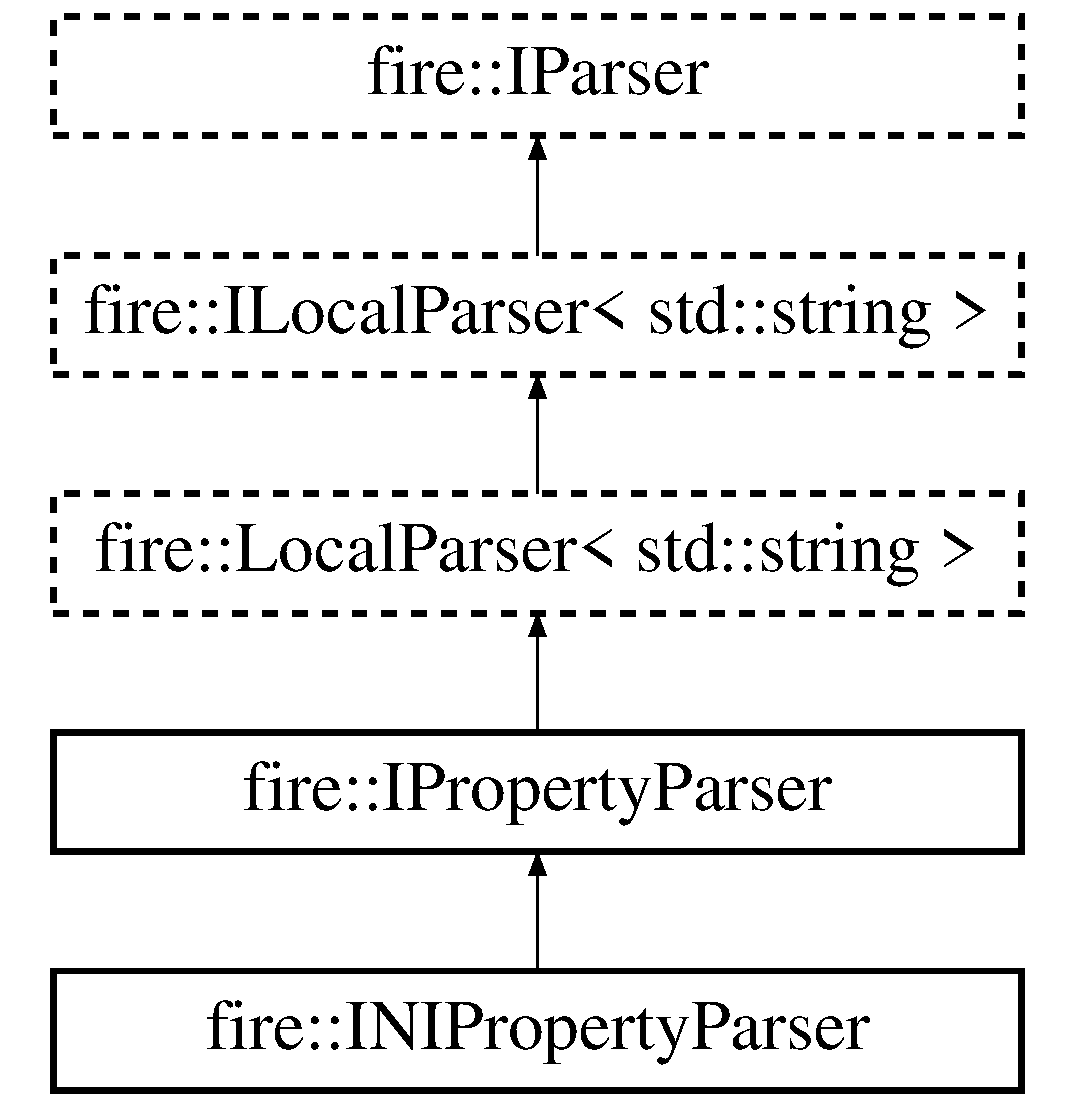
\includegraphics[height=5.000000cm]{a00822}
\end{center}
\end{figure}
\subsection*{Public Member Functions}
\begin{DoxyCompactItemize}
\item 
virtual const std\+::vector$<$ std\+::string $>$ \& \hyperlink{a00822_a34602687f9d1affac7bd842102d4a6aa}{get\+Property\+Block\+Names} ()=0
\item 
virtual const std\+::map$<$ std\+::string, std\+::string $>$ \& \hyperlink{a00822_a34201371cb36dd09e96a66242ececb86}{get\+Property\+Block} (const std\+::string \&name)=0
\end{DoxyCompactItemize}
\subsection*{Additional Inherited Members}


\subsection{Detailed Description}
This is an extension of the parser interface that focuses on parsing a set of properties. Properties are returned in blocks represented by maps.. 

\subsection{Member Function Documentation}
\mbox{\Hypertarget{a00822_a34201371cb36dd09e96a66242ececb86}\label{a00822_a34201371cb36dd09e96a66242ececb86}} 
\index{fire\+::\+I\+Property\+Parser@{fire\+::\+I\+Property\+Parser}!get\+Property\+Block@{get\+Property\+Block}}
\index{get\+Property\+Block@{get\+Property\+Block}!fire\+::\+I\+Property\+Parser@{fire\+::\+I\+Property\+Parser}}
\subsubsection{\texorpdfstring{get\+Property\+Block()}{getPropertyBlock()}}
{\footnotesize\ttfamily virtual const std\+::map$<$std\+::string, std\+::string$>$\& fire\+::\+I\+Property\+Parser\+::get\+Property\+Block (\begin{DoxyParamCaption}\item[{const std\+::string \&}]{name }\end{DoxyParamCaption})\hspace{0.3cm}{\ttfamily [pure virtual]}}

This operation returns the property block with the given name. 
\begin{DoxyParams}{Parameters}
{\em name} & the block name \\
\hline
\end{DoxyParams}
\begin{DoxyReturn}{Returns}
the property block with the given name 
\end{DoxyReturn}


Implemented in \hyperlink{a00814_a3591312590a66659ebd377cdde9ab9ad}{fire\+::\+I\+N\+I\+Property\+Parser}.

\mbox{\Hypertarget{a00822_a34602687f9d1affac7bd842102d4a6aa}\label{a00822_a34602687f9d1affac7bd842102d4a6aa}} 
\index{fire\+::\+I\+Property\+Parser@{fire\+::\+I\+Property\+Parser}!get\+Property\+Block\+Names@{get\+Property\+Block\+Names}}
\index{get\+Property\+Block\+Names@{get\+Property\+Block\+Names}!fire\+::\+I\+Property\+Parser@{fire\+::\+I\+Property\+Parser}}
\subsubsection{\texorpdfstring{get\+Property\+Block\+Names()}{getPropertyBlockNames()}}
{\footnotesize\ttfamily virtual const std\+::vector$<$std\+::string$>$\& fire\+::\+I\+Property\+Parser\+::get\+Property\+Block\+Names (\begin{DoxyParamCaption}{ }\end{DoxyParamCaption})\hspace{0.3cm}{\ttfamily [pure virtual]}}

This operation returns the names of the property blocks parsed from the source. \begin{DoxyReturn}{Returns}
the block names 
\end{DoxyReturn}


Implemented in \hyperlink{a00814_aed0f1f47111794659564dcddb4d25bc6}{fire\+::\+I\+N\+I\+Property\+Parser}.



The documentation for this class was generated from the following file\+:\begin{DoxyCompactItemize}
\item 
I\+Property\+Parser.\+h\end{DoxyCompactItemize}

\hypertarget{a00826}{}\section{fire\+:\+:Local\+Parser$<$ T $>$ Class Template Reference}
\label{a00826}\index{fire\+::\+Local\+Parser$<$ T $>$@{fire\+::\+Local\+Parser$<$ T $>$}}


{\ttfamily \#include $<$Local\+Parser.\+h$>$}

Inheritance diagram for fire\+:\+:Local\+Parser$<$ T $>$\+:\begin{figure}[H]
\begin{center}
\leavevmode
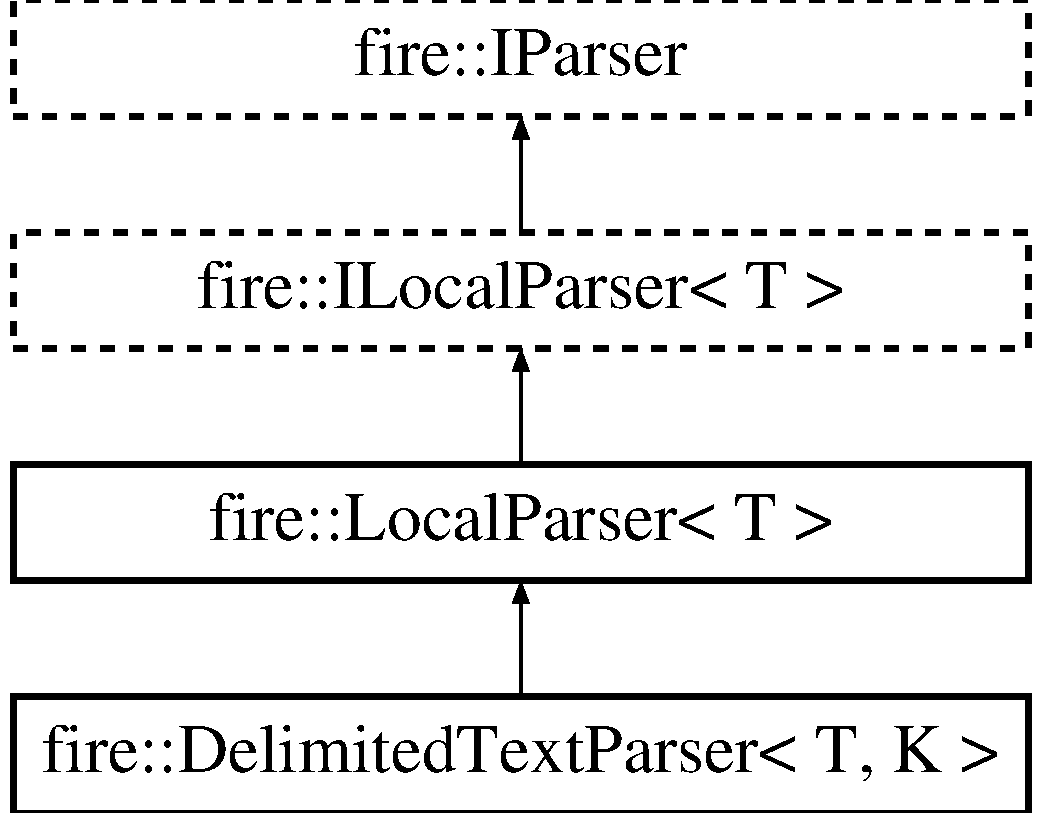
\includegraphics[height=4.000000cm]{a00826}
\end{center}
\end{figure}
\subsection*{Public Member Functions}
\begin{DoxyCompactItemize}
\item 
virtual void \hyperlink{a00826_afcaec6429fdd6e5d53642a32c001ff73}{set\+Source} (const std\+::string \&source)
\item 
virtual void \hyperlink{a00826_abd8929aea06c2dda40256d2e58236650}{parse} ()
\item 
virtual void \hyperlink{a00826_aed4357541f2ff7d46f8846bd07bb3c42}{set\+Source} (const std\+::istream \&source)
\item 
virtual const std\+::string \& \hyperlink{a00826_aedb7fe10911182525a719963b9b56726}{get\+Source} ()
\item 
virtual const std\+::istream \& \hyperlink{a00826_a9bf19a3cc9ae8ac0e6e7a0e7f6212cdc}{get\+Source\+Stream} ()
\item 
virtual std\+::shared\+\_\+ptr$<$ T $>$ \hyperlink{a00826_ab9016cca8e5dca516bb57c6a8e76607a}{get\+Data} ()
\item 
{\footnotesize template$<$$>$ }\\void \hyperlink{a00826_a34fd9ffb0196c612c75b5288ed5e219b}{parse} ()
\item 
{\footnotesize template$<$$>$ }\\void \hyperlink{a00826_ae904e264fe16708b3e434adea59e1b88}{parse} ()
\end{DoxyCompactItemize}
\subsection*{Protected Attributes}
\begin{DoxyCompactItemize}
\item 
std\+::string \hyperlink{a00826_acf921ee916266efe70be5b24bec37fce}{source\+File}
\item 
std\+::shared\+\_\+ptr$<$ T $>$ \hyperlink{a00826_af8f722c7e35378c69e76e4275d384d86}{data}
\end{DoxyCompactItemize}


\subsection{Detailed Description}
\subsubsection*{template$<$typename T$>$\newline
class fire\+::\+Local\+Parser$<$ T $>$}

The Local\+Parser$<$\+T$>$ is a templated parser that provides support for parsing local files of various types based only on the templated type.

This class works through {\itshape Explicit Specialization}, where subclasses are created using concrete types as template arguments instead of through direct inheritance. One important benefit of this approach to the author is that parsing with local files comes uniform and type-\/independent. For example,


\begin{DoxyCode}
LocalParser<UTKAstroNetwork> parser1;
LocalParser<ReacLib> parser2;

\textcolor{comment}{// Other work...}

network = parser1.parse();
rates = parser2.parse();
\end{DoxyCode}


Confer {\itshape C++ Templates\+: The Complete Guide} by Vandervoorde and Josuttis for full details on explicit specialization.

This class always assumes that its source is a file.

F\+I\+X\+M\+E! -\/ Specialization

Subclasses must always be sure that they implement \hyperlink{a00826_abd8929aea06c2dda40256d2e58236650}{parse()} and \hyperlink{a00826_afcaec6429fdd6e5d53642a32c001ff73}{set\+Source()} because default implementations are not provided. 

\subsection{Member Function Documentation}
\mbox{\Hypertarget{a00826_ab9016cca8e5dca516bb57c6a8e76607a}\label{a00826_ab9016cca8e5dca516bb57c6a8e76607a}} 
\index{fire\+::\+Local\+Parser@{fire\+::\+Local\+Parser}!get\+Data@{get\+Data}}
\index{get\+Data@{get\+Data}!fire\+::\+Local\+Parser@{fire\+::\+Local\+Parser}}
\subsubsection{\texorpdfstring{get\+Data()}{getData()}}
{\footnotesize\ttfamily template$<$typename T$>$ \\
virtual std\+::shared\+\_\+ptr$<$T$>$ \hyperlink{a00826}{fire\+::\+Local\+Parser}$<$ T $>$\+::get\+Data (\begin{DoxyParamCaption}{ }\end{DoxyParamCaption})\hspace{0.3cm}{\ttfamily [inline]}, {\ttfamily [virtual]}}

This operation returns a shared pointer to an instance of type T. \begin{DoxyReturn}{Returns}
a shared pointer holding an instance of type T that was parsed from the file. 
\end{DoxyReturn}


Implements \hyperlink{a00810_a0fc1446d106f0ab8daf8744a4bd29a65}{fire\+::\+I\+Local\+Parser$<$ T $>$}.

\mbox{\Hypertarget{a00826_aedb7fe10911182525a719963b9b56726}\label{a00826_aedb7fe10911182525a719963b9b56726}} 
\index{fire\+::\+Local\+Parser@{fire\+::\+Local\+Parser}!get\+Source@{get\+Source}}
\index{get\+Source@{get\+Source}!fire\+::\+Local\+Parser@{fire\+::\+Local\+Parser}}
\subsubsection{\texorpdfstring{get\+Source()}{getSource()}}
{\footnotesize\ttfamily template$<$typename T$>$ \\
virtual const std\+::string\& \hyperlink{a00826}{fire\+::\+Local\+Parser}$<$ T $>$\+::get\+Source (\begin{DoxyParamCaption}{ }\end{DoxyParamCaption})\hspace{0.3cm}{\ttfamily [inline]}, {\ttfamily [virtual]}}

This operation gets the data source for the parser. \begin{DoxyReturn}{Returns}
the name of the source 
\end{DoxyReturn}


Implements \hyperlink{a00818_ab55d2644dfa6d950d1f874e1e02df095}{fire\+::\+I\+Parser}.



Reimplemented in \hyperlink{a00814_ad02c9a530f20a706d7bb2554813e8d3a}{fire\+::\+I\+N\+I\+Property\+Parser}.

\mbox{\Hypertarget{a00826_a9bf19a3cc9ae8ac0e6e7a0e7f6212cdc}\label{a00826_a9bf19a3cc9ae8ac0e6e7a0e7f6212cdc}} 
\index{fire\+::\+Local\+Parser@{fire\+::\+Local\+Parser}!get\+Source\+Stream@{get\+Source\+Stream}}
\index{get\+Source\+Stream@{get\+Source\+Stream}!fire\+::\+Local\+Parser@{fire\+::\+Local\+Parser}}
\subsubsection{\texorpdfstring{get\+Source\+Stream()}{getSourceStream()}}
{\footnotesize\ttfamily template$<$typename T$>$ \\
virtual const std\+::istream\& \hyperlink{a00826}{fire\+::\+Local\+Parser}$<$ T $>$\+::get\+Source\+Stream (\begin{DoxyParamCaption}{ }\end{DoxyParamCaption})\hspace{0.3cm}{\ttfamily [inline]}, {\ttfamily [virtual]}}

This operation gets the data source for the parser as a stream if and only if it was set as such. \begin{DoxyReturn}{Returns}
source the stream of delimited text data 
\end{DoxyReturn}


Implements \hyperlink{a00818_ac94c7a288bf669322b93ba171c43f90e}{fire\+::\+I\+Parser}.

\mbox{\Hypertarget{a00826_ae904e264fe16708b3e434adea59e1b88}\label{a00826_ae904e264fe16708b3e434adea59e1b88}} 
\index{fire\+::\+Local\+Parser@{fire\+::\+Local\+Parser}!parse@{parse}}
\index{parse@{parse}!fire\+::\+Local\+Parser@{fire\+::\+Local\+Parser}}
\subsubsection{\texorpdfstring{parse()}{parse()}\hspace{0.1cm}{\footnotesize\ttfamily [1/3]}}
{\footnotesize\ttfamily template$<$$>$ \\
void \hyperlink{a00826}{fire\+::\+Local\+Parser}$<$ std\+::vector$<$ \hyperlink{a00766}{Species} $>$ $>$\+::parse (\begin{DoxyParamCaption}{ }\end{DoxyParamCaption})\hspace{0.3cm}{\ttfamily [virtual]}}

This operation parses a file that holds the basic species information for a thermonuclear network. 

Implements \hyperlink{a00818_af36ac6eedd8c27d2f418869193d7d03c}{fire\+::\+I\+Parser}.



Reimplemented in \hyperlink{a00806_a773fa7ed28cb9d8c384ad94bd81fc93f}{fire\+::\+Delimited\+Text\+Parser$<$ T, K $>$}.

\mbox{\Hypertarget{a00826_a34fd9ffb0196c612c75b5288ed5e219b}\label{a00826_a34fd9ffb0196c612c75b5288ed5e219b}} 
\index{fire\+::\+Local\+Parser@{fire\+::\+Local\+Parser}!parse@{parse}}
\index{parse@{parse}!fire\+::\+Local\+Parser@{fire\+::\+Local\+Parser}}
\subsubsection{\texorpdfstring{parse()}{parse()}\hspace{0.1cm}{\footnotesize\ttfamily [2/3]}}
{\footnotesize\ttfamily template$<$$>$ \\
void \hyperlink{a00826}{fire\+::\+Local\+Parser}$<$ vector$<$ \hyperlink{a00758}{Reaction} $>$ $>$\+::parse (\begin{DoxyParamCaption}{ }\end{DoxyParamCaption})\hspace{0.3cm}{\ttfamily [virtual]}}

This operation parses a file that holds the basic Reaction information for a thermonuclear network. 

Implements \hyperlink{a00818_af36ac6eedd8c27d2f418869193d7d03c}{fire\+::\+I\+Parser}.



Reimplemented in \hyperlink{a00806_a773fa7ed28cb9d8c384ad94bd81fc93f}{fire\+::\+Delimited\+Text\+Parser$<$ T, K $>$}.

\mbox{\Hypertarget{a00826_abd8929aea06c2dda40256d2e58236650}\label{a00826_abd8929aea06c2dda40256d2e58236650}} 
\index{fire\+::\+Local\+Parser@{fire\+::\+Local\+Parser}!parse@{parse}}
\index{parse@{parse}!fire\+::\+Local\+Parser@{fire\+::\+Local\+Parser}}
\subsubsection{\texorpdfstring{parse()}{parse()}\hspace{0.1cm}{\footnotesize\ttfamily [3/3]}}
{\footnotesize\ttfamily template$<$typename T$>$ \\
virtual void \hyperlink{a00826}{fire\+::\+Local\+Parser}$<$ T $>$\+::parse (\begin{DoxyParamCaption}{ }\end{DoxyParamCaption})\hspace{0.3cm}{\ttfamily [inline]}, {\ttfamily [virtual]}}

This operation directs the parser to parse its source. 

Implements \hyperlink{a00818_af36ac6eedd8c27d2f418869193d7d03c}{fire\+::\+I\+Parser}.



Reimplemented in \hyperlink{a00806_a773fa7ed28cb9d8c384ad94bd81fc93f}{fire\+::\+Delimited\+Text\+Parser$<$ T, K $>$}, \hyperlink{a00806_a686df5548771cae833d5e721442a821a}{fire\+::\+Delimited\+Text\+Parser$<$ T, K $>$}, and \hyperlink{a00814_a31b6bad01e65ed4bb5f1ba297616c641}{fire\+::\+I\+N\+I\+Property\+Parser}.

\mbox{\Hypertarget{a00826_afcaec6429fdd6e5d53642a32c001ff73}\label{a00826_afcaec6429fdd6e5d53642a32c001ff73}} 
\index{fire\+::\+Local\+Parser@{fire\+::\+Local\+Parser}!set\+Source@{set\+Source}}
\index{set\+Source@{set\+Source}!fire\+::\+Local\+Parser@{fire\+::\+Local\+Parser}}
\subsubsection{\texorpdfstring{set\+Source()}{setSource()}\hspace{0.1cm}{\footnotesize\ttfamily [1/2]}}
{\footnotesize\ttfamily template$<$typename T$>$ \\
virtual void \hyperlink{a00826}{fire\+::\+Local\+Parser}$<$ T $>$\+::set\+Source (\begin{DoxyParamCaption}\item[{const std\+::string \&}]{source }\end{DoxyParamCaption})\hspace{0.3cm}{\ttfamily [inline]}, {\ttfamily [virtual]}}

This operation sets the data source for the parser. 
\begin{DoxyParams}{Parameters}
{\em source} & the name of the source that the parser should parse. \\
\hline
\end{DoxyParams}


Implements \hyperlink{a00818_a0dbeff2b9bd8dbfb2aad7a424eef87d1}{fire\+::\+I\+Parser}.



Reimplemented in \hyperlink{a00814_a06793909bc707a69d0c5772b14bc946d}{fire\+::\+I\+N\+I\+Property\+Parser}.

\mbox{\Hypertarget{a00826_aed4357541f2ff7d46f8846bd07bb3c42}\label{a00826_aed4357541f2ff7d46f8846bd07bb3c42}} 
\index{fire\+::\+Local\+Parser@{fire\+::\+Local\+Parser}!set\+Source@{set\+Source}}
\index{set\+Source@{set\+Source}!fire\+::\+Local\+Parser@{fire\+::\+Local\+Parser}}
\subsubsection{\texorpdfstring{set\+Source()}{setSource()}\hspace{0.1cm}{\footnotesize\ttfamily [2/2]}}
{\footnotesize\ttfamily template$<$typename T$>$ \\
virtual void \hyperlink{a00826}{fire\+::\+Local\+Parser}$<$ T $>$\+::set\+Source (\begin{DoxyParamCaption}\item[{const std\+::istream \&}]{source }\end{DoxyParamCaption})\hspace{0.3cm}{\ttfamily [inline]}, {\ttfamily [virtual]}}

This operation sets the data source for the parser using a stream instead of a string. 
\begin{DoxyParams}{Parameters}
{\em source} & the stream of delimited text data \\
\hline
\end{DoxyParams}


Implements \hyperlink{a00818_a7748a633910e9bfc27411d6bd840496b}{fire\+::\+I\+Parser}.



\subsection{Member Data Documentation}
\mbox{\Hypertarget{a00826_af8f722c7e35378c69e76e4275d384d86}\label{a00826_af8f722c7e35378c69e76e4275d384d86}} 
\index{fire\+::\+Local\+Parser@{fire\+::\+Local\+Parser}!data@{data}}
\index{data@{data}!fire\+::\+Local\+Parser@{fire\+::\+Local\+Parser}}
\subsubsection{\texorpdfstring{data}{data}}
{\footnotesize\ttfamily template$<$typename T$>$ \\
std\+::shared\+\_\+ptr$<$T$>$ \hyperlink{a00826}{fire\+::\+Local\+Parser}$<$ T $>$\+::data\hspace{0.3cm}{\ttfamily [protected]}}

The shared pointer to the data set loaded by the \hyperlink{a00826_abd8929aea06c2dda40256d2e58236650}{parse()} operation. \mbox{\Hypertarget{a00826_acf921ee916266efe70be5b24bec37fce}\label{a00826_acf921ee916266efe70be5b24bec37fce}} 
\index{fire\+::\+Local\+Parser@{fire\+::\+Local\+Parser}!source\+File@{source\+File}}
\index{source\+File@{source\+File}!fire\+::\+Local\+Parser@{fire\+::\+Local\+Parser}}
\subsubsection{\texorpdfstring{source\+File}{sourceFile}}
{\footnotesize\ttfamily template$<$typename T$>$ \\
std\+::string \hyperlink{a00826}{fire\+::\+Local\+Parser}$<$ T $>$\+::source\+File\hspace{0.3cm}{\ttfamily [protected]}}

The source file name used if set\+Source(string) is called. 

The documentation for this class was generated from the following file\+:\begin{DoxyCompactItemize}
\item 
Local\+Parser.\+h\end{DoxyCompactItemize}

%--- End generated contents ---

% Index
\backmatter
\newpage
\phantomsection
\clearemptydoublepage
\addcontentsline{toc}{chapter}{Index}
\printindex

\end{document}
